% !TEX TS-program = pdflatexmk
% !BIB program = bibtex 
%%%%%%%%%%%%%%%%%%%% LN-Book.tex %%%%%%%%%%%%%%%%%%%%%%%%%%%%%
% Stand: 2025-06-01 ulgr
%%%%%%%%%%%%%%%% Springer-Verlag %%%%%%%%%%%%%%%%%%%%%%%%%%

\documentclass[% 
	,graybox
	,envcountsect			%% not working  
%	,evvcountsame			%% -- " --
%	,envcountresetsect		%% -- " --
%  	,sectrefs
% 	,natbib
%	,referee
	]{svmono}

% choose options for [] as required from the list
% in the Reference Guide

%\usepackage{mathptmx}
%\usepackage{helvet}
%\usepackage{courier}
%
\usepackage{type1cm}         

\usepackage{makeidx}         % allows index generation
\usepackage{graphicx}        % standard LaTeX graphics tool
                             % when including figure files
\usepackage{multicol}        % used for the two-column index
\usepackage[bottom]{footmisc}% places footnotes at page bottom

\usepackage{newtxtext}       % 
\usepackage[varvw]{newtxmath}       % selects Times Roman as basic font

%% -- Remarks und Examples
%% -- 
\spnewtheorem{remarks}[theorem]{Remarks}{\normalfont\bfseries}{\normalfont}
\spnewtheorem{examples}[theorem]{Examples}{\normalfont\bfseries}{\normalfont}

\spnewtheorem*{example*}{Example}{\normalfont\bfseries}{\normalfont}
\spnewtheorem*{examples*}{Examples}{\normalfont\bfseries}{\normalfont}
\spnewtheorem*{remark*}{Remark}{\normalfont\bfseries}{\normalfont}
\spnewtheorem*{remarks*}{Remark}{\normalfont\bfseries}{\normalfont}
\spnewtheorem*{definition*}{Definition}{\normalfont\bfseries}{\normalfont}

\spnewtheorem*{theorem*}{Theorem}{\normalfont\bfseries}{\itshape}
\spnewtheorem*{proposition*}{Proposition}{\normalfont\bfseries}{\itshape}
\spnewtheorem*{lemma*}{Lemma}{\normalfont\bfseries}{\itshape}
\spnewtheorem*{corollary*}{Corollary}{\normalfont\bfseries}{\itshape}

%% -- Nummer von Theorem etc. korrekt
%% --

\renewcommand\thetheorem{\thesection.\arabic{theorem}}
\renewcommand\theproposition{\thesection.\arabic{proposition}}
\renewcommand\thedefinition{\thesection.\arabic{definition}}
\renewcommand\thelemma{\thesection.\arabic{lemma}}
\renewcommand\thecorollary{\thesection.\arabic{corollary}}
\renewcommand\theremark{\thesection.\arabic{remark}}
\renewcommand\theremarks{\thesection.\arabic{remarks}}
\renewcommand\theexample{\thesection.\arabic{example}}
\renewcommand\theexamples{\thesection.\arabic{examples}}

\counterwithin{equation}{section}

%% -- Durchgehende Nummerierung
%% -- 
\makeatletter
\let\c@definition=\c@theorem 	% Make definition share the theorem counter
\let\c@example=\c@theorem 		% Make example share the theorem counter
\let\c@definition=\c@theorem 	% Make definition share the theorem counter
\let\c@examples=\c@theorem 		% Make examples share the theorem counter
\let\c@lemma=\c@theorem 		% Make lemma share the theorem counter
\let\c@corollary=\c@theorem 	% Make corollary share the theorem counter
\let\c@proposition=\c@theorem 	% Make proposition share the theorem counter
\let\c@remark=\c@theorem 		% Make proposition share the theorem counter
\let\c@remarks=\c@theorem 		% Make proposition share the theorem counter
\makeatother



%% -- Pakete etc.
%% -- 
%% -- Stand 2025/05/16
%% -- Unsere Pakete
%% --

\usepackage[english]{babel}					% Trennungen richtig
\usepackage{csquotes}						% \enquote{Text} US Variante 

%% -- Kein Einzug bei neuen Absatz und eine Leerzeile
%% --               
\usepackage[parfill]{parskip} 

\usepackage[inline,shortlabels]{enumitem}	% \begin{enumerate}[(i)] oder [(a)] 
 \setlist{parsep=.5em, labelindent=.5em, leftmargin=*}					

\usepackage{ragged2e}						% \RaggedRight = Flattersatz

%% --
\usepackage{tikz}
\usepackage{tikz-cd}
\usetikzlibrary{matrix,arrows.meta,calc}

%% --
\usepackage{comment}
\usepackage{xspace}

%% --
\usepackage{nomencl}
\makenomenclature
\renewcommand{\nomname}{List of Symbols}
\renewcommand{\nompreamble}{The next list describes several symbols that will be later used within the body of the document}

	
\usepackage{mathtools}
\usepackage{empheq}
\counterwithin{equation}{section}
\usepackage{colortbl} % Füge dies in den Präambel-Bereich ein

%% --
\usepackage{tikz}
\usepackage{tikz-cd}

%% -- Definitionen
%% --
%% -- Definitionen
%% -- Stand 2025/04/14
%% -- var-Symbole für griechisches Alphabet
%% --  Makro zum Tauschen von Symbolen 
%% --

\newcommand{\swapsymbols}[2]{%
  \let\temporaryhold#1%
  \let#1#2%
  \let#2\temporaryhold%
}

%% --  Griechische Buchstaben tauschen
\swapsymbols{\varepsilon}{\epsilon}
\swapsymbols{\varrho}{\rho}
\swapsymbols{\vartheta}{\theta}
\swapsymbols{\varphi}{\phi}

%% --  Vergleichsoperatoren tauschen
\swapsymbols{\leqslant}{\leq}
\swapsymbols{\geqslant}{\geq}


%% -- Zahlen
\newcommand{\N}{\mathbb{N}}		% Natuerliche Zahlen
\newcommand{\Z}{\mathbb{Z}}		% Ganze Zahlen
\newcommand{\Q}{\mathbb{Q}}		% Rationale Zahlen
\newcommand{\R}{\mathbb{R}}		% Reelle Zahlen
\newcommand{\C}{\mathbb{C}}		% Komplexe Zahlen
\newcommand{\K}{\mathbb{K}}		% Koerperzeichen
\newcommand{\T}{\mathbb{T}}		% Torus

%% -- Operatoren					
\DeclareMathOperator{\Id}{Id}
\DeclareMathOperator{\sign}{sign}				% signum-Operator
\newcommand{\im}{\ensuremath{\mathrm{i}}}		% imaginäre Konstante i
\renewcommand*{\Re}{\mathop{}\!\mathrm{Re}}		% Realteil
\renewcommand*{\Im}{\mathop{}\!\mathrm{Im}}		% Imaginärteil
\newcommand*{\supp}{\mathop{}\!\mathrm{supp}\,}  % Träger

%% -- Differential Allgemeine Abkuerzungen
%% --
\newcommand*{\diff}[1]{\mathop{}\!\mathrm{d}{#1}}	% \diff{s} = ds, 
\newcommand*{\ds}{\mathop{}\!\mathrm{d}{s}}       	% \ds = ds, 
\newcommand*{\dg}{\mathop{}\!\mathrm{d}{g}}       	% \dg = dg, 
\newcommand*{\dt}{\mathop{}\!\mathrm{d}{t}}       	% \dt = dt, 
\newcommand*{\dx}{\mathop{}\!\mathrm{d}{x}}       	% \dx = dx, 
\newcommand*{\dy}{\mathop{}\!\mathrm{d}{y}}       	% \dy = dy, 
\newcommand*{\dr}{\mathop{}\!\mathrm{d}{r}}       	% \dr = dr, 
\newcommand*{\dm}{\mathop{}\!\mathrm{d}{m}}       	% \dm = dm, 
\newcommand*{\du}{\mathop{}\!\mathrm{d}{u}}       	% \du = du, 

%% --
\newcommand{\LE}{\mathcal{L}(E)} 		% 
\renewcommand{\L}[1]{\mathcal{L}(#1)} 	% \L{C(K)} zum Beispiel
\newcommand{\BH}{\mathcal{B}(H)} 		% 
\newcommand{\ZE}{\mathcal{Z}(E)} 	% \ZE  Zentrum von E


\newcommand{\Fix}[1]{\mathop{}\mathrm{Fix}\left(#1\right)}		% \Fix{T} Fixraum
\newcommand{\rank}{\mathop{}\!\mathrm{rank}\,}		% 
\newcommand{\Kern}[1]{\mathop{}\mathrm{Ker}(#1)}


%% -- Enpunkt korrekt (momentan ignorieren)
\newcommand*{\eg}{e.g.,\xspace}
\newcommand*{\ie}{i.e.,\xspace}
\newcommand*{\resp}{resp.\xspace}
\newcommand*{\vs}{vs.\xspace}
\newcommand*{\cf}{cf.\xspace}

%% --
\newcommand{\CA}{$\mathrm{C}^{*}$}	% C*-Algebra
\newcommand{\WA}{$\mathrm{W}^{*}$}	% W*-Algbera

%%
\newcommand*{\TT}{\mathcal{T}}		% C_0-Semigroup
\newcommand*{\RR}{\mathcal{R}}		% Pseudo Resolvente
\newcommand*{\SG}{\mathcal{S}}	    % Semigroup
\newcommand*{\UG}{\mathcal{U}}	    % Implemented Semigroup
\newcommand*{\F}{\mathcal{F}}		% F-product
       
%% -- Angepasstes E/F und 1/3
%% -- 1/3

\newcommand*{\sfrac}[2]{\leavevmode\kern.1em%
       \raise.5ex\hbox{\scriptsize #1}%
       \kern-.1em/\kern-.15em%
       \lower.25ex\hbox{\scriptsize #2}}

\newcommand{\nfrac}[2]{\leavevmode\kern.1em%
       \raise.5ex\hbox{\scriptsize #1}%
       \kern-.1em/\kern-.15em%
       \lower.25ex\hbox{\scriptsize #2}}
       
%% -- E/F im Textmodus, sonst \sfrac{E}{F}
%% -- \trfac{E}{F}
%% -- 
\renewcommand{\tfrac}[2]{\raisebox{0.5ex}{#1}\big/\raisebox{-0.5ex}{#2}}
%%

%% -- Eins einer Algebra oder \1_{A} charakteristische Funktion
%% -- 

\usepackage{bbm}
\newcommand{\1}{\mathbbm{1}}

%%KGK
%\theoremstyle{definition}
%\newtheorem*{corollary*}{Corollary}

%% -- O-Spaces
\newcommand{\HO}{\mathcal{H}(O)} 		%  für Lotz
\newcommand{\WO}{\mathcal{W}(O)} 		%  für Lotz

%% -- Differential Allgemeine Abkuerzungen
%% --

\newcommand*{\ddp}{\mathop{}\!\mathrm{d}{p}}       	% \ddp = dp, 
\newcommand*{\dN}{\mathop{}\!\mathrm{d}{N}}       	% \dN = dN, 
\newcommand*{\ddt}{\mathop{}\!\mathrm\fraq{d}{dt}}   % \ddt = d/dt

\newcommand*{\lnm}{LNM1184: } % \LMN-BookCode









%% -- References
%% --

\usepackage{chapterbib}
\usepackage[square,numbers]{natbib}
%\bibliographystyle{spmpsci}



%\makeindex             % used for the subject index
\usepackage{imakeidx}
\makeindex[intoc, columns=2, options=-s svind.ist]                      
% please use the style svind.ist with
                       % your makeindex program
                       
%% --
%% -- https://www.uweziegenhagen.de/?p=3020	
%% -- Stand
%% --

\date{\LARGE Stand: \today}

%% -- Part A etc
%% -- A-I etc für \chapter
%% -- 1. für \section etc
%% --
\renewcommand\thepart{\Alph{part}}
\renewcommand\thechapter{\thepart-\Roman{chapter}}
\renewcommand\thesection{\arabic{section}}
\renewcommand\thesubsection{\thesection.\arabic{subsection}}

%% -- Wegen Überlappung im TOC
\usepackage{tocloft} 
\renewcommand\cftchapnumwidth{1cm}

%% -- \subsection nicht ins TOC
%% --
\setcounter{tocdepth}{1}

%% -- Für Links im PDF
%% --
\usepackage{hyperref}
\hypersetup{%
	,unicode	= false,
	,breaklinks = true	%
	,colorlinks	= true  %  Farbige Links false/true, für onlineversion true                                                           
	,urlcolor	= blue  %                                                              
	,citecolor	= blue  %                                                          
	,linkcolor	= blue	% oder black
	,hypertexnames=false
%  	,hidelinks 			% Vor dem Druck % entfernen
	}

%% -- 
%% -- nur die Dateien nutzen, 
%% -- die nicht auskommentiert sind (ohne %)
%% --

\includeonly{%
,./part-0/ln-dedication
%,./part-0/foreword
,./part-0/ln-preface
%,./part-0/acknowledgement
,./part-0/ln-symbols
%%%%% -- Part A
%%%%% --
,./part-a/part-a
,./part-a/chap-a1	%% -- final
,./part-a/chap-a2	%% -- final
,./part-a/chap-a3	%% -- final
,./part-a/chap-a4   %% -- final
%%%%,./part-a/appendix-a 
%%%% -- Part B
%%%% --
,./part-b/part-b	  
,./part-b/chap-b1  %% -- final
,./part-b/chap-b2  %% -- final
,./part-b/chap-b3  %% -- final
,./part-b/chap-b4  %% -- final
%%%,./part-b/appendix-b
%%% -- Part C 
%%% --
,./part-c/part-c
,./part-c/chap-c1	%% -- final
,./part-c/chap-c2	%% -- final
,./part-c/chap-c3
,./part-c/chap-c4
%%%%,./part-c/appendix-c
%%%% -- Part D
%%%% --
,./part-d/part-d
,./part-d/chap-d1
,./part-d/chap-d2
,./part-d/chap-d3
,./part-d/chap-d4
%%,./part-d/appendix-d
}
%% --
\begin{document}
%% --
\author{Wolfgang Arendt, Annette Grabosch, Günther Greiner, Ulrich Groh, Heinrich P. Lotz, Ulrich Moustakas, Rainer Nagel, Frank Neubrander, Ulf Schlotterbeck}
%% --
\title{One-parameter Semigroups of Positive Operators\\
		{\large{Edited by R. Nagel}}}
%% --
\subtitle{Lecture Notes in Mathematics\\ \\ 1184\\ \\Springer-Verlag\\ Berlin Heidelberg New York Tokyo}
%% --
\maketitle
%% --
\frontmatter%%%%%%%%%%%%%%%%%%%%%%%%%%%%%%%%%%%%%%%%%%%%%%%%%%%%%%
%%% -- part-0
% !TEX root = ../LN-Book.tex
%%%%%%%%%%%%%%%%%%%%%%% dedic.tex %%%%%%%%%%%%%%%%%%%%%%%%%%%%%%%%%
%
% dedication
% Stand: 2025/01/13 ulgr
% Use this file as a template for your own input.
%
%%%%%%%%%%%%%%%%%%%%%%%% Springer %%%%%%%%%%%%%%%%%%%%%%%%%%

\begin{dedication}
{\RaggedRight\Large 
This revised edition of \enquote{\emph{One-Parameter Semigroups of Positive Operators}} is dedicated to the memory 	of our 
co-authors, Heinrich P.~Lotz (1934--2010) and Ulf Schlotterbeck (1941--2021). 
Their contributions to the first edition remain an inspiration to us all. 
We miss their presence and remain grateful for the legacy they have left in this work.}
\end{dedication}





%\include{./part-0/foreword}
% !TEX root = ../LN-Book.tex
%%%%%%%%%%%%%%%%%%%%%%preface.tex%%%%%%%%%%%%%%%%%%%%%%%%%%%%%%%%%%%%%%%%%
% preface
% 2025/12/12
%
%%%%%%%%%%%%%%%%%%%%%%%% Springer %%%%%%%%%%%%%%%%%%%%%%%%%%

\preface

\section*{Preface to the Second Edition}
	
When the first edition of these lecture notes appeared in 1986, the theory of one-parameter semigroups of positive operators was undergoing rapid development, stimulated by applications in ergodic theory, evolution equations, stochastics, and mathematical physics. 
Our goal at the time was to provide a systematic and accessible account of the foundations and structure theory of positive semigroups, with particular emphasis on Banach lattices and $C^*$-algebras. 
We were gratified by the positive reception the volume received and the extent to which it found use in research and graduate instruction.

Over the past four decades, the mathematical community has continued to draw on the results and techniques developed in these notes. 
Despite the appearance of newer texts and the evolution of the field, this volume has remained widely cited and used---likely due to its thorough and methodical treatment of a core area in functional analysis. 
The sustained interest from both researchers and students has encouraged us to prepare this second edition.

We have preserved the structure and exposition of the original edition but have made a number of editorial improvements, including transferring the entire book into \LaTeX{}. 
Obvious misprints have been corrected, references have been updated where appropriate, and the notes at the end of each chapter have been significantly expanded in the chapter \emph{Updated Notes} to highlight subsequent developments. 
However, we have refrained from substantially altering the original content in order to retain the historical character and coherence of the text.

Two of our original co-authors, Heinrich P.~Lotz (1934--2010) and Ulf Schlotterbeck (1941--2021), sadly passed away in the years following the publication of the first edition. 
In addition, our former co-authors Annette Grabosch and Ulrich Moustakas are no longer engaged in active mathematical research at this time. 
To preserve the integrity and historical authorship of the original text, we have attributed all chapters to their original authors. 
Members of the present author team carefully reviewed these contributions for this second edition:
%% --
\begin{enumerate}[$\bullet$, wide, labelindent=.25em,itemsep=.25em]
\item 
The chapters originally written by Ulf Schlotterbeck were reviewed and updated by Rainer Nagel.

\item 
The chapters originally written by Heinrich P.~Lotz were reviewed and updated by Wolfgang Arendt.

\item 
The chapters originally written by Annette Grabosch and Ulrich Moustakas were reviewed and updated by G\"unther Greiner.

\end{enumerate}
%% --
The original authors of all other chapters participated directly in this new edition. 
We remain grateful for the foundational work of all nine original authors and hope that the clarity regarding authorship and review responsibilities will support the scholarly use of both editions.

We gratefully acknowledge the efforts of our co-author, Ulrich Groh, who guided the transfer of the manuscript into \LaTeX{}, with the assistance of Klaus-Georg Kuhn and the support of Claude, an artificial intelligence model developed by Anthropic.



It is our hope that this new edition will continue to serve as a valuable resource for those working in operator theory, functional analysis, and their many applications. We remain deeply grateful to our colleagues and readers who have provided feedback and encouragement over the years.
%% --

%% --
\section*{Preface to the First Edition}
 
As early as 1948 in the first edition of his fundamental treatise on \emph{Semigroups and Functional Analysis}, E.~Hille expressed the need for 
 
 \begin{quote}
 \textit{\ldots developing an adequate theory of transformation semigroups operating in partially ordered spaces} (l.c., Foreword). 
 \end{quote}
 
 In the meantime the theory of one-parameter semigroups of positive linear operators has grown continuously. 
 Motivated by problems in probability theory and partial differential equations W.~Feller (1952) and R.~S.~Phillips (1962) laid the first cornerstones by characterizing the generators of special positive semigroups. 
 In the 60's and 70's the theory of positive operators on ordered Banach spaces was built systematically and is well documented in the monographs of H.~H.~Schaefer (1974) and A.~C.~Zaanen (1983). 
 But in this process the original ties with the applications and, in particular, with initial value problems were at times obscured. 
 Only in recent years an adequate and up-to-date theory emerged, largely based on the techniques developed for positive operators and thus recombining the functional analytic theory with the investigation of Cauchy problems having positive solutions to each positive initial value. 
 Even though this development --- in particular with respect to applications to concrete evolution equations in transport theory, mathematical biology, and physics --- is far from being complete, the present volume is a first attempt to shape the multitude of available results into a coherent theory of one-parameter semigroups of positive linear operators on ordered Banach spaces.
 
 The book is organized as follows.
 We concentrate our attention on three subjects of semigroup theory: \emph{characterization}, \emph{spectral theory} and \emph{asymptotic behavior}. 
 By \emph{characterization}, we understand the problem of describing special properties of a semigroup, such as positivity, through the generator. 
 By \emph{spectral theory} we mean the investigation of the spectrum of a generator. 
 \emph{Asymptotic behavior} refers to the orbits of the initial values under a given semigroup and phenomena such as stability.
 
 This program (characterization, spectral theory, asymptotic behavior) is worked out on four different types of underlying spaces.
 
 %% --
 \begin{enumerate}[label=(\Alph*)]
 \item 
 On Banach spaces---Here we present the background for the subsequent discussions related to order.
 
 \item 
 On spaces $C_{0}(X)$ ($X$ locally compact), which constitute an important class of ordered Banach spaces and where our results can be presented in a form which makes them accessible also for the non-expert in order-theory.
 
 \item 
 On Banach lattices, which admit a rich theory and are still sufficiently general as to include many concrete spaces appearing in analysis; e.g., $C_0(X)$, $\mathcal{L}^p(k)$ or $l^p$.
 
 \item 
 On non-commutative operator algebras such as \CA- or \WA-algebras, which are not lattice ordered but still possess an interesting order structure of great importance in mathematical physics.
 
 \end{enumerate}
 %% --
 In each of these cases we start with a short collection of basic results and notations, so that the contents of the book may be visualized in the form of a $4 \times 4$ matrix in a way which will allow \enquote{row readers} (interested in semigroups on certain types of spaces) and \enquote{column readers} (interested in certain aspects) to find a path through the book corresponding to their interest.
 
 We display this matrix, together with the names of the authors contributing to the subjects defined through this scheme.
 %% --
 \begin{table}[ht]
 \centering
 %% --
 \begin{tabular}{l|c|c|c|c|}
 \cline{2-5}
  & I & II & III & IV \\
  & Basic & Characterization & Spectral & Asymptotics \\
  & Results &  & Theory & \\
 \hline
 \multicolumn{1}{|l|}{A. Banach} & R. Nagel & W. Arendt & G. Greiner & F. Neubrander \\
 \multicolumn{1}{|l|}{Spaces} & U. Schlotterbeck & H. P. Lotz & R. Nagel & \\
 \hline
 \multicolumn{1}{|l|}{B. $C_0(X)$} & R. Nagel & W. Arendt & G. Greiner & A. Grabosch \\
 \multicolumn{1}{|l|}{} & U. Schlotterbeck & & & G. Greiner \\
 \multicolumn{1}{|l|}{} & & & & U. Moustakas \\
 \multicolumn{1}{|l|}{} & & & & F. Neubrander \\
 \hline
 \multicolumn{1}{|l|}{C. Banach} & R. Nagel & W. Arendt & G. Greiner & A. Grabosch \\
 \multicolumn{1}{|l|}{Lattices} & U. Schlotterbeck & & & G. Greiner \\
 \multicolumn{1}{|l|}{} & & & & U. Moustakas \\
 \multicolumn{1}{|l|}{} & & & & R. Nagel \\
 \multicolumn{1}{|l|}{} & & & & F. Neubrander \\
 \hline
 %\rowcolor{darkgreen}
 \multicolumn{1}{|l|}{D. Operator} & U. Groh & U. Groh & U. Groh & U. Groh \\
 %\rowcolor{darkgreen}
 \multicolumn{1}{|l|}{Algebras} & & & & \\
 \hline
 \end{tabular}
 \end{table}
 %% --
 This \enquote{matrix of contents} has been an indispensable guide line in our discussions on the scope and the spirit of the various contributions. 
 However, we would not have succeeded in completing this manuscript, as a collection of independent contributions (personally accounted for by the authors), under less favorable conditions than we have actually met. 
 For one thing, Rainer Nagel was an unfaltering and undisputed spiritus rector from the very beginning of the project. 
 On the other hand we gratefully acknowledge the influence of Helmut H.~Schaefer and his pioneering work on order structures in analysis. 
 It was the team spirit produced by this common mathematical background which, with a little help from our friends, made it possible to overcome most difficulties.
 
 We have prepared the manuscript with the aid of a word processor, but we confess that without the assistance of 
 Klaus-Georg Kuhn the pitfalls of such a system would have been greater than its benefits.
 \vspace{.5cm}
 \begin{flushright}\noindent
 ${}$\hfill {\itshape The authors} \\
 \end{flushright}
 
 \vspace{.5cm}
 \begin{center}
 \includegraphics{./part-0/apparaetle.jpg}
 \end{center}




%\include{./part-0/acknowledgement}
%% --
\tableofcontents
%% --
 % !TEX root = ../LN-Book.tex

\nomenclature{$E_{\R}$, $E_{\C} = E$}{real, complex Banach lattice}
\nomenclature{$E_{+}$}{positive cone}
\nomenclature{$E'$}{dual Banach space}
\nomenclature{$E^*$}{semigroup dual}
\nomenclature{$E_{F}^{T}$}{$ \F $-product of $ E $ with respect to semigroup $\TT$}
\nomenclature{$E_{F}$}{$ \F $-product of $ E $}
\nomenclature{$E_{f}$}{see C-I,4}
\nomenclature{$(E,\phi)$}{see C-I,4}
\nomenclature{$E\otimes F$}{tensor product}
\nomenclature{$\LE$}{Banach space of bounded linear operators on E}
\nomenclature{$\mathcal{Z}(E)$}{center of E}
\nomenclature{$E_{n}$}{$ n $-th Sobolev space}
\nomenclature{$B(H)$}{\WA-algebra of bounded linear operators on a Hilbert space $ H $}
\nomenclature{$S(M)$}{state space of C*-algebra M}
\nomenclature{$M_{+}$}{positive cone of C*-algebra M}
\nomenclature{$M_{*}$}{predual}
\nomenclature{$M^{sa}$}{self-adjoint part}
\nomenclature{$M_{n}$}{C*-algebra of nxn-matrices}
\nomenclature{AC}{absolutely continuous functions}
\nomenclature{BV}{functions of bounded variation}
\nomenclature{K}{compact topological space}
\nomenclature{X}{locally compact topological space}
\nomenclature{$C(K)$, $C(K,E)$}{continuous functions (with values in E)}
\nomenclature{$C_{o}(X)$, $C_{o}(X,E)$}{continuous functions vanishing at infinity with values in E}
\nomenclature{$C^{b}(X)$}{bounded continuous functions}
\nomenclature{$C_{uu}(X)$}{uniformly continuous functions}
\nomenclature{$C^{n}$, $C^{(n)}$}{continuous differentiable functions (n-times)}
\nomenclature{$C_{c}^{\infty}(\mathbb{R}^n)$}{infinitely differentiable functions with compact support}
\nomenclature{$L^{p}(\mu)$}{p-integrable functions}
\nomenclature{$S(\mathbb{R}^n)$}{Schwartz space}
\nomenclature{$M(K)$}{regular Borel measures}
\nomenclature{$M_{b}(X)$}{bounded regular Borel measures}
\nomenclature{$T = (T(t))_{t\geq0}$}{(one-parameter) semigroup}
\nomenclature{$T|$}{subspace (reduced) semigroup}
\nomenclature{$T/$}{quotient semigroup}
\nomenclature{Fix$(T)$}{fixed space of T}
\nomenclature{$A$}{generator}
\nomenclature{$A'$}{adjoint}
\nomenclature{$A^*$}{adjoint generator}
\nomenclature{$\sigma(A)$}{spectrum}
\nomenclature{$\rho(A)$}{resolvent set}
\nomenclature{$\sigma_{ess}(A)$}{essential spectrum}
\nomenclature{$\sigma_{b}(A)$}{boundary spectrum}
\nomenclature{$P\sigma(A)$}{point spectrum}
\nomenclature{$P\sigma_{b}(A)$}{boundary point spectrum}
\nomenclature{$A\sigma(A)$}{approximate point spectrum}
\nomenclature{$R\sigma(A)$}{residual spectrum}
\nomenclature{$\omega = \omega(A) = \omega(T)$}{growth bound}
\nomenclature{$s(A)$}{spectral bound}
\nomenclature{$\omega_{I}(A)$}{growth bound of solution of (ACP)}
\nomenclature{$\omega(f)$}{growth bound of $T(\cdot)f$}
\nomenclature{$r(T)$}{spectral radius}
\nomenclature{$\omega_{ess}(A)$}{essential growth bound}
\nomenclature{$r_{ess}(T)$}{essential spectral radius}
\nomenclature{$R(\lambda,A)$}{resolvent operator}
\nomenclature{$I^{d}$, $\{I^{d}\}_{d=1}^{dd}$}{orthogonal band of I (of $I^{d}$)}
\nomenclature{$\wedge$}{infimum}
\nomenclature{$\vee$}{supremum}
\nomenclature{$|T|$}{modulus of regular operator}
\nomenclature{$\hat{f}$, $\check{f}$}{Fourier (inverse Fourier) transformation}
\nomenclature{$d\rho(f)$}{subdifferential of $\rho$ in f}
\nomenclature{$dN(f)$}{subdifferential of norm in f}
\nomenclature{$dN^{+}(f)$}{subdifferential of canonical half-norm in f}
\nomenclature{im}{range}
\nomenclature{ker}{null-space}
\nomenclature{Im}{imaginary part}
\nomenclature{Re}{real part}
\nomenclature{$\text{Re}f$, $\text{Im}f$}{see C-I,7}
\nomenclature{$\text{Re}T$, $\text{Im}T$}{see C-I,7}
\nomenclature{$\bar{f}$}{complex conjugate of f}
\nomenclature{$S_{f}$}{signum operator with respect to f}
\nomenclature{sign $f$}{signum of f}
\nomenclature{$f^{[n]}$}{see C-II,2.2}
\nomenclature{$|f|$}{absolute value of f}
\nomenclature{$f^{+}$}{positive part of f}
\nomenclature{$f^{-}$}{negative part of f}
\nomenclature{Id}{identity operator}
\nomenclature{$M_{p}$}{multiplication operator}
\nomenclature{1}{function identically 1}
\nomenclature{$1_{C}$}{characteristic function of set C}
\nomenclature{$\delta_{x}$}{Dirac measure in x}
\nomenclature{tr}{trace}
\nomenclature{span M}{linear subspace generated by M}
\nomenclature{$S(\alpha)$}{sector in complex plane}
\nomenclature{(ACP)}{abstract Cauchy problem}
\nomenclature{(P)}{positive minimum principle}
\nomenclature{(P')}{B-II,1.21}
\nomenclature{(K)}{Kato's (equality) inequality}
\nomenclature{(RCP)}{retarded Cauchy problem}
\nomenclature{(RE)}{retarded equation}
\nomenclature{(T)}{translation property}
 \printnomenclature
%%
\mainmatter%%%%%%%%%%%%%%%%%%%%%%%%%%%%%%%%%%%%%%%%%%%%%%%%%%%%%%%
%
%% -- Part-A

% !TEX root = ../../LN-Book.tex
%% -- Stand 2025-11-28 
%% -- ulgr
%% -- Part A
%% --

\begin{partbacktext}
\part[One-parameter Semigroups on Banach Spaces]{One-parameter Semigroups on Banach Spaces }
\end{partbacktext}
% \setcounter{chapter}{0} 
%% Stand 2025-04-24 ulgr
%% --
\chapter{Basic Results on Semigroups on Banach Spaces}\label{chap:a1}
\index{Basic Results}
%% --
{\Large
\vspace*{-.75cm}
by \\[.25em]
Rainer Nagel and Ulf Schlotterbeck 
\vspace{.75cm}
\\
}
%% --
Since the basic theory of one-parameter semigroups can be found in several excellent books (\eg \citet{davies:1980}, \citet{goldstein:1985a}, \citet{pazy:1983} or \citet{hillephillips:1957}), we do not want to give a self-contained introduction to this subject here.
It may however be useful to fix our notation, to collect briefly some important definitions and results (Section 1), to present a list of \emph{standard examples} in Section~\ref{sec:a1-2} %(Section 2) 
and to discuss standard constructions of new semigroups from a given one in Section~\ref{sec:a1-3} on p.\,\pageref{sec:a1-3}. %(Section 3).

In the entire chapter we denote by $E$ a (real or) complex Banach space and consider one-parameter semigroups of bounded linear operators $T(t)$ on $E$.
By this we understand a subset $\{T(t) \colon  t \in \R_{+}\}$ of $\LE$, usually written as $(T(t))_{t\geq0}$, such that
%% --
\begin{align*}
	T(0) &= \Id, \\
	T(s+t) &= T(s) \cdot T(t) \text{ for all $s$, $t \in \R_{+}$.}
\end{align*}
%% --
In more abstract terms this means that the map $t \mapsto T(t)$ is a homomorphism from the additive semigroup $(\R_{+},+)$ into the multiplicative semigroup $(\LE,\cdot)$.
Similarly, a one-parameter group $(T(t))_{t\in\R}$ will be a homomorphic image of the group $(\R,+)$ in $(\LE,\cdot)$.
%% --
\section{Standard Definitions and Results}\label{sec:a1-1}
\index{Basic Results!Standard Definitions and Results}
%% --
We consider a one-parameter semigroup $(T(t))_{t \geq 0}$ on a Banach space $E$ 
and observe that the domain $\R_{+}$ and the range $\LE$ of the (semigroup) homomorphism $\tau \colon t \mapsto T(t)$ are topological semigroups for the natural topology on $\R_{+}$ and any one of the standard operator topologies on $\LE$.
We single out the strong operator topology on $\LE$ and require $\tau$ to be continuous.
%% --
\begin{definition}\label{def:a1-1.1}
A one-parameter semigroup $(T(t))_{t\geq0}$ is called \emph{strongly continuous} if the map $t \mapsto T(t)$ is continuous for the strong operator topology on $\LE$, \eg
%% --
\[
	\lim_{t\to t_{0}} \|T(t)f - T(t_{0})f\| = 0
\]
%% --
for every $f \in E$ and $t$, $t_{0} \geq 0$.
\end{definition}
%% --
Clearly one defines in a similar way \emph{weakly continuous}, \resp \emph{uniformly continuous} (compare A-II, Def. 1.19) semigroups, but since we concentrate on the strongly continuous case we agree on the following terminology.
%% --
\begin{quote}
If not stated otherwise, a \emph{semigroup} is a strongly continuous one-parameter semigroup of bounded linear operators.
\end{quote}
%% --
Next we collect a few elementary facts on the continuity and boundedness of one-parameter semigroups.
%% --
\begin{remarks*}\label{rem:a1-1.2}
%% --
\begin{enumerate}[(i), wide, labelsep=1em, itemindent=\parindent]

\item 
A one-parameter semigroup $(T(t))_{t \geq 0}$ on a Banach space $E$ is strongly continuous if and only if for any $f \in E$ it is true that $T(t)f \to f$ if $t \to 0$.

\item 
For every strongly continuous semigroup there exist constants $M \geq 1$, $w \in \R$ such that $\|T(t)\| \leq M \cdot e^{wt}$ for every $t \geq 0$.
\item If $(T(t))_{t\geq0}$ is a one-parameter semigroup such that $\|T(t)\|$ is bounded for $0 < t \leq \delta$ then it is strongly continuous if and only if $\lim_{t \to 0} T(t)f = f$ for every $f$ in a total subset of $E$.
\end{enumerate}
\end{remarks*}
%% --
The exponential estimate from Remark~\ref{rem:a1-1.2}\,(ii) for the growth of $\|T(t)\|$ can be used to define an important characteristic of the semigroup.
%% --
\begin{definition}\label{def:a1-1.3}
By the growth bound (or type) of the semigroup $(T(t))_{t\geq0}$ we understand the number
%% --
\begin{align*}\label{eq:a1-1.1}
\omega_{0} \coloneqq{}& \inf\{w \in \R \colon \text{There exists } M \in \R_{+} \text{ such that } \|T(t)\| \leq Me^{wt} \text{ for } t \geq 0\} \\
={}& \lim_{t\to\infty} \frac{1}{t}\log\|T(t)\| = \inf_{t>0} \frac{1}{t}\log\|T(t)\| \notag .
\end{align*}
%% --
\end{definition}
%% --
\noindent Particularily important are semigroups such that for every $t \geq 0$ we have $\|T(t)\| \leq M$ (\emph{bounded semigroups}) or $\|T(t)\| \leq 1$ (\emph{contraction semigroups}).
In both cases we have $\omega_{0} \leq 0$.

It follows from the subsequent examples and from Def.~\ref{def:a1-1.3} that $\omega_{0}$ may be any number $ -\infty \leq \omega < +\infty$.
Moreover the reader should observe that the infimum in Def.~\ref{def:a1-1.3} need not be attained and that $M$ may be larger than $1$ even for bounded semigroups.
%% --
\begin{examples}\label{ex:a1-1.4}
%% --
\begin{enumerate}[(i), wide, labelsep=1em, itemindent=\parindent]

\item 
Take $E = \mathbb{C}^2$, 
\[
	A = \begin{pmatrix}0 & 1\\0 & 0\end{pmatrix} 
	\quad \text{and} \quad 
	T(t) = e^{tA} = \begin{pmatrix}1 & t\\0 & 1\end{pmatrix} .
\]
%
Then for the $\ell^{1}$-norm on $E$ we obtain $\|T(t)\| = 1 + t$, hence $(T(t))_{t\geq0}$ is an unbounded semigroup having growth bound $\omega_{0} = 0$.

\item 
Take $E = L^1(\R)$ and for $f \in E$, $t \geq 0$ define
%% --
\begin{align*}
T(t)f(x) \coloneqq 
	\begin{cases}
		2\cdot f(x+t) & \text{if } x \in [-t,0] \\
		f(x+t) & \text{otherwise}.
	\end{cases}
\end{align*}
%% --
Each $T(t)$, $t > 0$, satisfies $\|T(t)\| = 2$ as can be seen by taking $f := \chi_{[0,t]}$.
Therefore $(T(t))_{t \geq 0}$ is a strongly continuous semigroup which is bounded, hence has $\omega_{0} = 0$, but the constant $M$ in (1.3) cannot be chosen to be $1$.

\end{enumerate}
\end{examples}
%% --
The most important object associated to a strongly continuous semigroup $(T(t))_{t\geq0}$ is its \emph{generator} which is obtained as the (right)derivative of the map $t \mapsto T(t)$ at $t = 0$.
Since for strongly continuous semigroups the functions $t \mapsto T(t)f$, $f \in E$, are continuous but not always differentiable, we have to restrict our attention to those $f \in E$ for which the desired derivative exists.
We then obtain the \emph{generator} as a not necessarily everywhere defined operator.

\begin{definition}\label{def:a1-1.5}
To every semigroup $(T(t))_{t \geq 0}$ there belongs an operator $(A,D(A))$, called the \emph{generator} and defined on the \emph{domain}
%% --
\begin{align*}
	D(A) \coloneqq{} & \{f \in E \colon \lim_{h\to0} \frac{T(h)f - f}{h} \text{ exists in $E$}\} \\
    \text{ by} \\
	Af \coloneqq{} & \lim_{h\to0} \frac{T(h)f - f}{h} \quad (f \in D(A)).
\end{align*}
%% --
\end{definition}
%% --
%\noindent 
Clearly, $D(A)$ is a linear subspace of $E$ and $A$ is linear from $D(A)$ into $E$.
Only in certain special cases (see \ref{subsec:a1-2.1}) the generator
is everywhere defined and therefore bounded (use Prop.~\ref{prop:a1-1.9}\,(ii)) on p.\,\pageref{prop:a1-1.9}). %Prop.1.9(i)).
In general, the precise extent of the domain $D(A)$ is essential for the characterization of the generator.
But since the domain is canonically associated to the generator of a semigroup, we shall write in most cases $A$ instead of $(A,D(A))$.

As a first result we collect some information on the domain of the generator.
%% --
\begin{proposition}\label{prop:a1-1.6}
For the generator $A$ of a semigroup $(T(t))_{t \geq 0}$ on a Banach space~$E$ the following assertions hold.
%% --
\begin{enumerate}[(i)]
\item
If $f \in D(A)$, then $T(t)f \in D(A)$ for every $t \geq 0$.

\item
The map $t \mapsto T(t)f$ is differentiable on $\R_{+}$ if and only if $f \in D(A)$.
In that case one has
%% --
\begin{equation}\label{eq:a1-1.2}
    \frac{d}{dt} T(t)f = AT(t)f = T(t)Af .
\end{equation}
%% --
\item
For every $f \in E$ and $t > 0$ the element $\int_0^t T(s)f\ds$ belongs to $D(A)$ and one has
%% --
\begin{equation}\label{eq:a1-1.3}
    A\int_0^t T(s)f \ds = T(t)f - f  .
\end{equation}
%% --
\item
If $f \in D(A)$, then
%% --
\begin{equation}\label{eq:a1-1.4}
    \int_0^t T(s)Af \ds = T(t)f - f  .
\end{equation}

%% --
\item
The domain $D(A)$ is dense in $E$.
\end{enumerate}
%% --
\end{proposition}
%% --
The identity \eqref{eq:a1-1.2} is of great importance and shows how semigroups are related to certain Cauchy problems.
We state this explicitly in the following theorem.
%% --
\begin{theorem}\label{thm:a1-1.7}
Let $(A,D(A))$ be the generator of a strongly continuous semigroup $(T(t))_{t \geq 0}$ on the Banach space $E$.
Then the \emph{abstract Cauchy problem}
%% --
\begin{equation}\label{eq:a1-1.5}
\frac{d}{dt}\xi(t) = A\xi(t), \quad \xi(0) = f_{0}
\end{equation}
%% --
has a unique solution $\xi \colon \R_{+} \to D(A)$ in $C^1(\R_{+},E)$ for every $f_{0} \in D(A)$.
In fact, this solution is given by $\xi(t) \coloneqq T(t)f_{0}$.
\end{theorem}
%% --
For more on the relation of semigroups to abstract Cauchy problems we refer to A-II,Section 1.
Here we only point out that the above theorem implies that a semigroup is uniquely determined by its generator.

While the generator is bounded only for uniformly continuous semigroups (see Sec.\,\ref{sec:a1-2} below), it always enjoys a weaker but useful property.
%% --
\begin{definition}\label{def:a1-1.8}
An operator $B$ with domain $D(B)$ on a Banach space $E$ is called \emph{closed} if $D(B)$ endowed with the \emph{graph norm}
%% --
\[
    \|f\|_{B} \coloneqq \|f\| + \|Bf\|
\]
%% --
becomes a Banach space.
Equivalently, $(B,D(B))$ is closed if and only if its \emph{graph} $\{(f,Bf) \colon f \in D(B)\}$ is closed in $E \times E$, \ie
%% --
\[
    f_{n} \in D(B), f_{n} \to f \text{ and } Bf_{n} \to g \text{ implies } f \in D(B) \text{ and } Bf = g.
\]
%% --
\end{definition}
%% --
It is clear from this definition that the \emph{closedness} of an operator $B$ depends very much on the size of the domain $D(B)$.
For example, a bounded and densely defined operator $(B,D(B))$ is closed if and only if $D(B) = E$.

On the other hand it may happen that $(B,D(B))$ is not closed but has a closed \emph{extension} $(C,D(C))$, \ie  $ D(B) \subseteq D(C)$ and $Bf = Cf$ for every $f \in D(B)$.
In that case, $B$ is called \emph{closable}, a property which is equivalent to
%% --
\[
    f_{n} \in D(B), f_{n} \to 0 \text{ and } Bf_{n} \to g \text{ implies } g = 0.
\]
%% --
The smallest closed extension of $(B,D(B))$ will be called the \emph{closure} $\overline{B}$ with domain $D(\overline{B})$.
In other words, the graph of $\overline{B}$ is the closure of $\{(f,Bf) \colon f \in D(B)\}$ in $E \times E$.

Finally we call a subset $D_{0}$ of $D(B)$ a \emph{core} for $B$ if $D_{0}$ is $\|\cdot\|_{B}$-dense in $D(B)$.
This means that a closed operator is determined (via closure) by its restriction to a core in its domain.

We now collect the fundamental topological properties of semigroup generators, their domains (see also A-II,Cor.1.34) and their resolvents.
%% --
\begin{proposition}\label{prop:a1-1.9}
For the generator $A$ of a strongly continuous semigroup $(T(t))_{t \geq 0}$ the following hold.
%% --
\begin{enumerate}[(i)]
\item 
The generator $A$ is a closed operator.

\item
If a subspace $D_{0}$ of the domain $D(A)$ is dense in $E$ and $(T(t))$-invariant, then it is a core for $A$.
% --
\item Define $D(A^{n}) \coloneqq \{f \in D(A^{n-1}) \colon Af \in D(A^{n-1})\}$, $D(A^{1}) = D(A)$.
Then $D(A^{\infty}) \coloneqq \bigcap_{n \in \N} D(A^{n})$ is dense in $E$ and a core for $A$.
\end{enumerate}
%% --
\end{proposition}
%% --
\begin{example}\label{ex:a1-1.10}
Property (iii) above does not hold for general densely defined closed operators.
Take $E = C\left[ 0,1 \right]$, $D(B) = C^{1}\left[ 0,1 \right]$ and $Bf = q \cdot f'$ for some nowhere differentiable function $q \in C\left[ 0,1 \right]$.
Then $B$ is closed, but $D(B^{2}) = \{0\}$.
\end{example}
%% --
\begin{proposition}\label{prop:a1-1.11}
For the generator $A$ of a strongly continous semigroup on a Banach space $E$ the following hold.

If $\int_{0}^{\infty} e^{-\lambda t}T(t)f \, dt$ exists for every $f \in E$ and some $\lambda \in \mathbb{C}$, then $\lambda \in \rho(A)$ and $R(\lambda,A)f = \int_{0}^{\infty} e^{-\lambda t}T(t)f \, dt$.
In particular,
%% --
\begin{equation}\label{eq:a1-1.7}
R(\lambda,A)^{n+1}f = \frac{(-1)^{n}}{n!}\left(\frac{d}{d\lambda}\right)^{n} R(\lambda,A)f = \int_{0}^{\infty} e^{-\lambda t}\frac{t^{n}}{n!}T(t)f \, dt
\end{equation}
%% --
for every $f \in E$, $n \geq 0$ and $\lambda \in \mathbb{C}$ with $\Re(\lambda) > \omega$.
\end{proposition}
%% --
\begin{remarks}\label{rem:a1-1.12}
%% --
\begin{enumerate}[(i), wide, labelsep=1em, itemindent=\parindent]
%% --
\item 
For continuous Banach space valued functions such as $t \mapsto T(t)f$ we consider the Riemann integral and define 
%% --
\[
\int_{0}^{\infty}T(t)f \, \dt 
\quad \text{as} \quad
\lim_{t \to \infty}\int_{0}^{t}T(s)f \, \ds .
\]
%% --
Sometimes such integrals for strongly continuous semigroups are written as $\int_{a}^{b}T(t) \, dt$ but understood in the strong sense.

\item 
Since the generator $(A,D(A))$ determines the semigroup uniquely, we will speak occasionally of the growth bound of the generator instead of the semigroup, \ie we write $\omega_{0} = \omega_{0}(A) = \omega_{0}((T(t))_{t \geq 0}$.

\item 
For one-parameter groups it might seem to be more natural to define the generator as the \emph{derivative} rather than just the \emph{right derivative} at $t = 0$.
This yields the same operator as the following result shows.

The strongly continuous semigroup $(T(t))_{t \geq 0}$ with generator $A$ can be extended to a strongly continuous one-parameter group $(U(t))_{t \in \R}$ if and only if $-A$ generates a semigroup $(S(t))_{t \geq 0}$.

In that case $(U(t))_{t \in \R}$ is obtained as
%% --
\[
    U(t) = \begin{cases}
        T(t) & \text{for } t \geq 0 ,\\
        S(-t) & \text{for } t \leq 0 .
    \end{cases}
\]
%% --
We refer to \citet[Prop.1.14]{davies:1980} for the details.

\end{enumerate}
\end{remarks}
%% --
\section{Standard Examples}\label{sec:a1-2}
\index{Basic Results!Standard Examples}
%\index{Standard Examples}
%% --
In this section we list and discuss briefly the most basic examples of semigroups together with their generators.
These semigroups will reappear throughout this book and will be used to illustrate the theory.
We start with the class of semigroups mentioned after Definition~\ref{def:a1-1.1} on p.~\pageref{def:a1-1.1}.
%% --
\subsection{Uniformly Continuous Semigroups}\label{subsec:a1-2.1}
%\index{Uniformly Continuous Semigroups}
%\index{Semigroups!Uniformly Continuous}
\index{Standard Examples!Uniformly Continuous Semigroups}
%% --
It follows from elementary operator theory that for every bounded operator $A$ in  $\LE$ the sum
%% --
\[
    \sum_{n=0}^{\infty} \frac{t^{n}A^{n}}{n!} = \colon e^{tA}
\]
%% --
exists and determines a unique uniformly continuous (semi)group $(e^{tA})_{t \in \R}$ having $A$ as its generator.
Conversely, any uniformly continuous semigroup is of this form.

If the semigroup $(T(t))_{t \geq 0}$ is uniformly continuous, then $\frac{1}{t}\int_{0}^{t} T(s) \ds$ uniformly converges to $T(0) = \Id$ as $t \to 0$.
Therefore for some $t' > 0$ the operator $\frac{1}{t'}\int_{0}^{t'} T(s) \ds$ is invertible and every $f \in E$ is of the form $f = \frac{1}{t'}\int_{0}^{t'} T(s)g \ds$ for some $g \in E$.
But these elements belong to $D(A)$ by (1.3), hence $D(A) = E$.
Since the generator $A$ is closed and everywhere defined, it must be bounded.

Remark that bounded operators are always generators of groups, not just semigroups.
Moreover, the growth bound $\omega$ satisfies $|\omega| \leq \|A\|$ in this situation.

The above characterization of the generators of uniformly continuous semigroups as the bounded operators shows that these semigroups are---at least in many aspects---rather simple objects.
%% --
\subsection{Matrix Semigroups}\label{subsec:a1-2.2}
%\index{Matrix Semigroups}
%\index{Semigroups!Matrix}
\index{Standard Examples!Matrix Semigroups}
%% --
The above considerations expecially apply in the situation $E = \mathbb{C}^{n}$.
If $n = 2$ and $A = (a_{ij})_{2 \times 2}$ the following explicit formulas for $e^{tA}$ might be of interest.

Set
%% --
\begin{enumerate*}[(i)]
\item
$s \coloneqq \text{trace } A$, 

\item
$d \coloneqq \text{det } A$

\item
and $D \coloneqq (s^{2} - 4d)^{1/2}$.
\end{enumerate*}
%% --
Then if  $D \neq 0$
%% -- 
\[
    e^{tA} = 
        e^{ts/2} \cdot [D^{-1}2\sinh(tD/2) \cdot A + (\cosh(tD/2) - sD^{-1}\sinh(tD/2)) \cdot \Id] 
\]
%% --
and if $D=0$
%% --
\[
	e^{ts/2} \cdot [tA + (1 - ts/2) \cdot \Id] .
\]
%% --
\subsection{Multiplication Semigroups}\label{subsec:a1-2.3}
\index{Standard Examples!Multiplication Semigroups}
%% --
Many Banach spaces appearing in applications are Banach spaces of (real or) complex valued functions over a set $X$.
%% --
As the most standard examples of these \enquote{function spaces}, we mention the space $C_{0}(X)$ of all continuous complex valued functions vanishing at infinity on a locally compact space $X$, or the spaces $L^{p}(X,\Sigma,\mu)$, $1 \leq p \leq \infty$, of all (equivalence classes of) $p$-integrable functions on a $\sigma$-finite measure space $(X,\Sigma,\mu)$.

On these function spaces $E = C_{0}(X)$, \resp $E = L^{p}(X,\Sigma,\mu)$, there is a simple way to define \emph{multiplication operators}.

Take a continuous, \resp measurable function $q \colon X \to \mathbb{C}$ and define
%% --
\[
    M_{q}f \coloneqq q \cdot f, \quad \text{\ie} \quad M_{q}f(x) 
    \coloneqq q(x) 	\cdot f(x) \quad \text{for } x \in X 
\]
%% --
and for every $f$ in the \emph{maximal} domain $D(M_{q}) \coloneqq \{g \in E \colon q \cdot g \in E\}$.

This natural domain is a dense subspace of $C_{0}(X)$, \resp $L^{p}(X,\Sigma,\mu)$, for $1 \leq p < \infty$.
Moreover, $(M_{q},D(M_{q}))$ is a closed operator.
This is easy in case $E = C_{0}(X)$.

For $E = L^{p}(X,\Sigma,\mu)$, $1 \leq p < \infty$, we consider a sequence $(f_{n}) \subset E$ such that $\lim_{n \to \infty} f_{n} = f \in E$ and $\lim_{n \to \infty} qf_{n} = \colon g \in E$.
Choose a subsequence $(f_{n(k)})_{k \in \N}$ such that $\lim_{k \to \infty} f_{n(k)}(x) = f(x)$ and $\lim_{k \to \infty} q(x)f_{n(k)}(x) = g(x)$ for $\mu$-almost every $x \in X$.
Then $g = q \cdot f$ and $f \in D(M_{q})$, \ie $M_{q}$ is closed.

For such multiplication operators many properties can be checked quite directly.
For example, the following statements are equivalent.
%% --
\begin{enumerate}[(a)]
\item 
$M_{q}$ is bounded.

\item 
$q$ is ($\mu$-essentially) bounded.
\end{enumerate}
%% --
One has $\|M_{q}\| = \|q\|_{\infty}$ in this situation.
Observe that on spaces $C(K)$, $K$ compact, there are no densely defined, unbounded multiplication operators.

By defining the multiplication semigroups
%% --
\[
    T(t)f(x) \coloneqq \exp(t \cdot q(x))f(x), \quad x \in X, f \in E,
\]
%% --
one obtains the following characterizations.
%% --
\begin{proposition}\label{prop:a1-2.3}
\index{Standard Examples!Multiplication Operators}
%% --
Let $M_{q}$ be a multiplication operator on $E = C_{0}(X)$ or $E = L^{p}(X,\Sigma,\mu)$, $1 \leq p < \infty$.
Then the properties (a) and (b), \resp (a') and (b'), are equivalent.
%% --
\begin{enumerate}[(a)]
\item 
	$M_{q}$ generates a strongly continuous semigroup.

\item 
	$\sup\{\Re( q(x)) \colon x \in X \} < \infty$.

\item[(a')] 
	$M_{q}$ generates a uniformly continuous semigroup.

\item[(b')] 
	$\sup\{|q(x)| \colon x \in X \} < \infty$.
\end{enumerate}
%% --
\end{proposition}
%% --
As a consequence one computes the growth bound of a multiplication semigroup as
%% --
\[
    \omega_{0} = \sup\{\Re(q(x)) \colon x \in X\} 
\]
%% --
in the case $E = C_{0}(X)$ and 
%% --
\[
    \omega_{0} = \mu\text{-ess-}\sup\{\Re(q(x)) \colon x \in X\} 
\]
%% --
in the case  $E = L^{p}(\mu)$.
It is a nice exercise to characterize those multiplication operators which generate strongly continuous groups.

We point out that the above results cover the cases of sequence spaces such as $c_{0}$ or $\ell^{p}$, $1 \leq p < \infty$.
An abstract characterization of generators of multiplication semigroups will be given in C-II,Thm.5.13.
%% --
\subsection{Translation (Semi)Groups}\label{subsec:a1-2.4}
\index{Standard Examples!Translation Semigroups}
%% --
Let $E$ to be one of the following function spaces $C_{0}(\R_{+})$, $C_{0}(\R)$ or $L^{p}(\R_{+})$, $L^{p}(\R)$ for $1 \leq p < \infty$.
Define $T(t)$ to be the (left) translation operator
%% --
\[
    T(t)f(x) \coloneqq f(x+t)
\]
%% --
for $x$ ,, $ t \in \R_{+}$, \resp $x, t \in \R$ and $f \in E$.
Then $(T(t))_{t \geq 0}$ is a strongly continous semigroup, \resp group of contractions on $E$ and its generator is the first derivative $\frac{d}{dx}$ with \emph{maximal} domain.
In order to be more precise we have to distinguish the cases $E = C_{0}$ and $E = L^{p}$.
%% -- 

The generator of the translation (semi)group on $E = C_{0}(\R_{+})$ is 
%% --
\begin{align*}
    Af & \coloneqq \frac{d}{\dx}f = f' \\
    D(A) &\coloneqq \{f \in E \colon f \text{ differentiable and } f' \in E\}.
\end{align*}
%% --
\begin{proof}
For $f \in D(A)$ it follows that for every $x \in \R_{(+)}$
%% --
\[
    \lim_{h \to 0} \frac{T(h)f(x) - f(x)}{h} = \lim_{h \to 0} \frac{f(x+h) - f(x)}{h} \text{ exists}
\]
%% --
(uniformly in $x$) and coincides with $Af(x)$.
Therefore $f$ is differentiable and $f' \in E$.

On the other hand, take $f \in E$ differentiable such that $f' \in E$.
Then
%% --
\[
    \left|\frac{f(x+h) - f(x)}{h} - f'(x)\right| \leq \frac{1}{h}\int_{x}^{x+h}|f'(y) - f'(x)|\,\dy,
\]
%% --
where the last expression tends to zero uniformly in $x$ as $h \to 0$.
Thus $f \in D(A)$ and $f' = Af$.
\end{proof}
%% --
The generator of the translation (semi)group on $E = L^{p}(\R_{+})$, $1 \leq p < \infty$, is
%% --
\begin{align*}
    Af &\coloneqq \frac{d}{\dx}f = f', \\
    D(A) &\coloneqq \{f \in E \colon f \text{ absolutely continuous}, f' \in E\}.
\end{align*}
%% --
\begin{proof}
Take $f \in D(A)$ such that $\lim_{h \to 0} \frac{1}{h}(T(h)f - f) = g \in E$.
Since integration is continuous, we obtain for every $a$, $b \in \R_{(+)}$ that
%% --
\begin{equation*}\label{eq:a1-2.1}
(*) \quad \frac{1}{h}\int_{b+h}^{b} f(x) \dx - \frac{1}{h}\int_{a+h}^{a} f(x) \dx = \int_{a}^{b} \frac{f(x+h) - f(x)}{h} \dx
\end{equation*}
%% --
converges to $\int_{a}^{b} g(x) \dx$ as $h \to 0+$.
But for almost all $a, b$ the left hand side of $(*)$ converges to $f(b) - f(a)$.
By redefining $f$ on a nullset we obtain
%% --
\[
    f(y) = \int_{a}^{y} g(x)\dx + f(a), \quad y \in \R_{(+)},
\]
%% --
which is an absolutely continuous function whose derivative is (almost everywhere) equal to $g$.

On the other hand, let $f$ be absolutely continuous such that $f' \in L^{p}$.
Then
%% --
\begin{align*}
    \lim_{h \to 0} \int \left|\frac{f(x+h) - f(x)}{h} - f'(x)\right|^{p} \dx 
    &= \lim_{h \to 0} \int \left|\frac{1}{h}\int_{0}^{h} (f'(x+s) - f'(x)) \ds\right|^{p} \dx \\
    &= \lim_{h \to 0} \int \left|\int_{0}^{1} (f'(x+uh) - f'(x)) \du\right|^{p} \dx \\
    &\leq \lim_{h \to 0} \int \int_{0}^{1} |f'(x+uh) - f'(x)|^{p} \du \dx \\
    &= \int_{0}^{1} \lim_{h \to 0} \int |f'(x+uh) - f'(x)|^{p} \dx \du = 0,
\end{align*}
%% --
hence $f \in D(A)$.
\end{proof}
%% --
\subsection{Rotation Groups}\label{subsec:a1-2.5}
\index{Standard Examples!Rotation Groups}
%% --
On $E = C(\Gamma)$, \resp $E = L^{p}(\Gamma,m)$, $1 \leq p < \infty$, $m$ Lebesgue measure we have canonical groups defined by rotations of the unit circle $\Gamma$ with a certain period, \ie for $0 < \tau \in \R$ the operators
%% --
\[
    R_{\tau}(t)f(z) \coloneqq f(e^{2\pi it/\tau}\cdot z), \quad z \in \Gamma
\]
%% --
yield a group $(R_{\tau}(t))_{t \in \R}$ having period $\tau$, \ie $R_{\tau}(\tau) = \Id$.
As in Example 2.4 one shows that its generator has the form
%% --
\begin{align*}
    D(A) &= \{f \in E \colon f \text{ absolutely continuous}, f' \in E\}, \\
    Af(z)&= (2\pi i/\tau) \cdot z \cdot f'(z).
\end{align*}
%% --
An isomorphic copy of the group $(R_{\tau}(t))_{t \in \R}$ is obtained if we consider $E = \{f \in C\left[ 0,1 \right] \colon f(0) = f(1)\}$, \resp $E = L^{p}(\left[ 0,1 \right])$ and the group of \emph{periodic translations}
%% --
\[
    T(t)f(x) \coloneqq f(y) \quad \text{for $y \in \left[ 0,1 \right], y = x+t \bmod 1$} 
\]
%% --
with generator
%% --
\[
    D(A) \coloneqq \{f \in E \colon f \text{ absolutely continuous}, f' \in E\},
    \quad Af \coloneqq f'.
\]
%% --
\subsection{Nilpotent Translation Semigroups}\label{subsec:a1-2.6}
\index{Standard Examples!Nilpotent Translation Semigroups}
%% --
Take $E = L^{p}([0,\tau],m)$ for $1 \leq p < \infty$ and define
%% --
\[
    T(t)f(x) \coloneqq \begin{cases}
        f(x+t) & \text{if } x+t \leq \tau \\
        0 & \text{otherwise.}
    \end{cases}
\]
%% --
Then $(T(t))_{t\geq 0}$ is a semigroup satisfying $T(t) = 0$ for $t \geq \tau$.
Its generator is still the first derivative $A = \frac{d}{\dx}$, but with domain is 
%% --
\[
D(A) = \{f \in E \colon f \text{ absolutely continuous}, f' \in E, f(\tau) = 0\}.
\]
%% --
In fact, if $f \in D(A)$, then $f$ is absolutely continuous with $f' \in E$.
By Prop.~\ref{prop:a1-1.6}\,(i) on p.\,\pageref{prop:a1-1.6} it follows that $T(t)f$ is absolutely continuous and hence $f(\tau) = 0$.
%% --
\subsection{One-dimensional Diffusion Semigroup}\label{subsec:a1-2.7}
\index{Standard Examples!One-dimensional Diffusion Semigroup}
%% --
For the second derivative 
%% --
\[
    Bf(x) \coloneqq \frac{d^{2}}{dx^{2}}f(x) = f''(x)
\]
%% --
we take the domain
%% --
\[
    D(B) \coloneqq \{f \in C^{2}\left[ 0,1 \right] \colon f'(0) = f'(1) = 0\}
\]
%% --
in the Banach space $E = C\left[ 0,1 \right]$.
Then $D(B)$ is dense in $C\left[ 0,1 \right]$, but closed for the graph norm.
Obviously, each function
%% --
\[
    e_{n}(x) \coloneqq \cos \pi nx, \quad n \in \mathbb{Z},
\]
%% --
is contained in $D(B)$ and is an eigenfunction of $B$ pertaining to the eigenvalue $\lambda_{n} \coloneqq -\pi^{2}n^{2}$.
The linear hull $\text{span }\{e_{n} \colon n \in \mathbb{Z}\} = \colon E_{0}$ forms a subalgebra of $D(B)$ which by the Stone-Weierstrass theorem is dense in $E$.

We now use $e_{n}$ to define bounded linear operators 
%
\[
	e_{n} \otimes e_{n} \colon f \mapsto \left(\int_{0}^{1} f(x)e_{n}(x) \dx \right)e_{n} 
		= ( f | e_{n} ) e_{n} %\langle f,e_{n}\rangle e_{n}
\]
%% -- 
satisfying $\|e_{n} \otimes e_{n}\| \leq 1$ and
$(e_{n} \otimes e_{n})(e_{m} \otimes e_{m}) = \delta_{n,m}(e_{n} \otimes e_{n})$ for $n \in \mathbb{Z}$.

For $t > 0$ we define
%% --
\begin{align*}
T(t) \coloneqq{}& \sum_{n \in \mathbb{Z}} \exp(-\pi^{2}n^{2}t) \cdot e_{n} \otimes e_{n} \\
		={}& e_{0} \otimes e_{0} + 2\sum_{n=1}^{\infty} \exp(-\pi^{2}n^{2}t) \cdot e_{n} \otimes e_{n},
\end{align*}
or
%% --
\begin{align*}
    T(t)f(x) &= \int_{0}^{1} k_{t}(x,y)f(x)dy \\
    \text{where } k_{t}(x,y) &= 1 + 2\sum_{n=1}^{\infty} \exp(-\pi^{2}n^{2}t) \cos\pi nx \cos\pi ny .
\end{align*}
%% --
The Jacobi identity
%% --
\begin{align*}
    w_{t}(x) &\coloneqq 1/(4\pi t)^{\frac{1}{2}} \sum_{m \in \mathbb{Z}} \exp(-(x+2m)^{2}/4t) \\
    &= \frac{1}{2} + \sum_{n \in \N} \exp(-\pi^{2}n^{2}t) \cos\pi nx
\end{align*}
%% --
and trigonometric relations show that
%% --
\[
    k_{t}(x,y) = w_{t}(x+y) + w_{t}(x-y)
\]
%% --
which is a positive function on $\left[ 0,1 \right]^{2}$.
Therefore $T(t)$ is a bounded operator on $C\left[ 0,1 \right]$ with
%% --
\[
    \|T(t)\| = \|T(t)\1\| = \sup_{x \in \left[ 0,1 \right]} \int_{0}^{1} k_{t}(x,y)dy = 1 .
\]
%% --
From the behavior of $T(t)$ on the dense subspace $E_{0}$ it follows that $(T(t))_{t \geq 0}$ with $T(0) = \Id$ is a strongly continuous semigroup on $E$ and its generator $A$ coincides with $B$ on $E_{0}$.
Finally, we observe that $E_{0}$ is a core for $(A,D(A))$ by Prop.1.9(ii).

Consequently, $(T(t))_{t \geq 0}$ is the semigroup generated by the closure of the second derivative with domain $D(B)$.
%% --
\subsection{n-dimensional Diffusion Semigroup}\label{subsec:a1-2.8}
\index{Standard Examples!$n$-dimensionalDiffusion Semigroup}
%% --
On $E = L^{p}(\R^{n})$, $1 \leq p \leq \infty$, the operators
%% --
\begin{align*}
    T(t)f(x) \coloneqq{}& (4\pi t)^{-n/2} \int_{\R^{n}} \exp(-|x-y|^{2}/4t)f(y)dy \\
    ={}& \mu_{t}*f(x)
\end{align*}
%% --
for $x \in \R^{n}$, $t > 0$ and $\mu_{t}(x) \coloneqq (4\pi t)^{-n/2} \exp(-|x|^{2}/4t)$ form a strongly continuous semigroup:

In fact the integral exists for every $f \in L^{p}(\R^{n})$ since $\mu_{t}$ is an element of the Schwartz space $S(\R^{n})$ of all rapidly decreasing smooth functions on $\R^{n}$.

Moreover,
%% --
\[
    \|T(t)f\|_{p} \leq \|\mu_{t}\|_{1}\|f\|_{p} = \|f\|_{p}
\]
%% --
by Young's inequality, \citet[p.28]{reedsimon:1975}, hence $\|T(t)\| \leq 1$ for every $t > 0$.
Next we observe that $S(\R^{n})$ is dense in $E$ and invariant under each $T(t)$.
%% --
Therefore we can apply the Fourier transformation $F$ which leaves $S(\R^{n})$ invariant and yields
%% --
\[
    F(\mu_{t}*f) = (2\pi)^{n/2} F(\mu_{t}) \cdot F(f) = (2\pi)^{n/2} \hat{\mu}_{t}\cdot\hat{f}
\]
%% --
where $f \in S(\R^{n})$, $\hat{f} = Ff \in S(\R^{n})$.

In other words, $F$ transforms $(T(t)\vert_{ S(\R^{n})})_{t \geq 0}$ into a multiplication semigroup on $S(\R^{n})$ which is pointwise continuous for the usual topology of $S(\R^{n})$.
The generator, \ie the right derivative at $0$, of this semigroup is the multiplication operator
%% --
\[
    B\hat{f}(x) \coloneqq -|x|^{2}\hat{f}(x) \quad (x \in \R^{n})
\]
%% --
for every $f \in S(\R^{n})$.

Applying the inverse Fourier transformation and observing that the topology of $S(\R^{n})$ is finer than the topology induced from $L^{p}(\R^{n})$, we obtain that $(T(t))_{t \geq 0}$ is a semigroup which is strongly continuous (use Rem.~\ref{rem:a1-1.2}\,(iii) on p.\,\pageref{rem:a1-1.2}). %ark 1.2, (3)).

Its generator $A$ coincides with
%% --
\[
    \Delta f(x) = \sum_{i=1}^{n} \frac{\partial^{2}}{\partial x_{i}^{2}} f(x_{1},\ldots,x_{n})
\]
%% --
for every $f \in S(\R^{n})$.
Since $S(\R^{n})$ is $(T(t))$-invariant, we have determined the generator on a core of its domain (see Prop.1.9.ii).
In particular, the above semigroup \emph{solves} the initial value problem for the \emph{heat equation}
%% --
\[
    \frac{\partial}{\partial t} f(x,t) = \Delta f(x,t), \quad f(x,0) = f_{0}(x), \quad x \in \R^{n}.
\]
%% --
For the analogous discussion of the unitary group on $L^{2}(\R^{n})$ generated by
%% --
\[
    C \coloneqq \im\Delta
\]
%% --
we refer to Section IX.7 in \citet{reedsimon:1975}. %[Reed-Simon (1975]).

Analogous examples to \ref{subsec:a1-2.7} are valid in $L^{p}\left[ 0,1 \right]$, \resp to 
\ref{subsec:a1-2.8} in $C_{0}(\R^{n})$.
%% --
\section{Standard Constructions}\label{sec:a1-3}
\index{Basic Results!Standard Constructions}
%% --
Starting with a semigroup $(T(t))_{t \geq 0}$ on a Banach space $E$ it is possible to construct new semigroups on spaces naturally associated with $E$.
Such constructions will be important technical devices in many of the subsequent proofs.
Although most of these constructions are rather routine, we present in the sequel a systematic account of them for the convenience of the reader.

We always start with a semigroup $(T(t))_{t \geq 0}$ on a Banach space $E$, and denote its generator by $A$ on the domain $D(A)$.
%% --
\subsection{Similar Semigroups}\label{subsec:a1-3.0}
\index{Standard Constructions!Similar Semigroups}
%% --
There is an easy way how to obtain different (but isomorphic) 
%% --
semigroups out of a given semigroup $(T(t))_{t \geq 0}$ on a Banach space $E$.

Let $V$ be an isomorphism from $E$ onto $E$.
Then $S(t) \coloneqq VT(t)V^{-1}$, $t \geq 0$, defines a strongly continuous semigroup.
If $A$ is the generator of $(T(t))_{t \geq 0}$ then
%% --
\[
    B \coloneqq VAV^{-1} \text{ with domain } D(B) \coloneqq \{f \in E \colon V^{-1}f \in D(A)\}
\]
%% --
is the generator of $(S(t))_{t \geq 0}$.
%% --
\subsection{The Rescaled Semigroup}\label{subsec:a1-3.1}
\index{Standard Constructions!Rescaled Semigroup}
%% --
For fixed $\lambda \in \mathbb{C}$ and $\alpha > 0$ the operators
%% --
\[
    S(t) \coloneqq \exp(\lambda t)T(\alpha t)
\]
%% --
yield a new semigroup having generator
%% --
\[
    B \coloneqq \alpha A + \lambda \Id \text{ with } D(B) = D(A) .
\]
%% --
This \emph{rescaled semigroup} enjoys most of the properties of the original semigroup and the same is true for the corresponding generators.
However, by using this procedure certain constants associated with $(T(t))_{t \geq 0}$ and $A$ can be normalized.
For example, by this rescaling we may in many cases suppose without loss of generality that the growth bound $\omega_{0}$ is zero.

Another application is the following.
For $\lambda \in \mathbb{C}$ and $S(t) \coloneqq \exp(-\lambda t)T(t)$ the formulas \emph{(1.3)} and \emph{(1.4)} yield:
%% --
\begin{align*}
    e^{-\lambda t}T(t)f - f &= (\lambda-A) \int_{0}^{t} e^{-\lambda s}T(s)f \ds \text{ or }\notag \\
    (e^{\lambda t}-T(t))f &= (\lambda-A) \int_{0}^{t} e^{\lambda(t-s)}T(s)f \ds \quad \text{for } f \in E, %\tag{3.1}
\end{align*}
%% --
and
%% --
\begin{align*}
    e^{-\lambda t}T(t)f - f &= \int_{0}^{t} e^{-\lambda s}T(s)(\lambda-A)f \ds  \text{or}\notag \\
    \notag \\
    (e^{\lambda t} - T(t))f &= \int_{0}^{t} e^{\lambda(t-s)}T(s)(\lambda-A)f \ds \quad \text{for } f \in D(A). %\tag{3.2}
\end{align*}
%% --
%% --
\subsection{The Subspace Semigroup}\label{subsec:a1-3.2}
\index{Standard Constructions!Subspace Semigroup}
%% --
Assume $F$ to be a closed $(T(t))$-invariant or, equivalently, $R(\lambda,A)$-invariant for 
$\lambda \in \C$, 
$ \Re(\lambda) > \omega_{0}$, subspace of $E$.
Then the semigroup $(T(t)_{|})_{t \geq 0}$ of all restrictions $T(t)_{|} \coloneqq T(t)_{|\,F}$ is strongly continuous on $F$.
If $(A,D(A))$ denotes the generator of $(T(t))_{t \geq 0}$ it follows from the $(T(t))$-invariance and closedness of $F$ that $A$ maps $D(A) \cap F$ into $F$.
Therefore
%% --
\[
    A_{|} \coloneqq A_{| (D(A)\cap F)} \text{ with domain } D(A_{|}) \coloneqq D(A) \cap F
\]
%% --
is the generator of $(T(t)_{|})$.
%
Conversely, if $F$ is a closed \emph{linear subspace} of $E$ with $A(D(A) \cap F) \subset F$ such that 
$A_{|}$ is a generator on $F$, then $F$ is $(T(t))$-invariant.

An $A$-invariant subspace need not necessarily be $(T(t))$-invariant:
Take for example the translation group with $T(t)f(x) = f(x+t)$ on $E = C_{0}(\R)$ and $F \coloneqq \{f \in E \colon f(x) = 0 \text{ for } x \leq 0\}$.
%% --
\subsection{The Quotient Semigroup}\label{subsec:a1-3.3}
\index{Standard Constructions!Quotient Semigroup}
%% --
Let $F$ be a closed $(T(t))$-invariant subspace of $E$ and consider the quotient space $ E_{/}\coloneqq \nfrac{E}{F} $ with quotient map $q \colon E \to E_{/}$. 
The quotient operators
%% --
\[
    T(t)_{/}q(f) \coloneqq q(T(t)f), \quad f \in E,
\]
%% --
are well defined and form a strongly continuous semigroup $(T(t)_{/})_{t \geq 0}$ on $E_{/}$.
For the generator $(A_{/},D(A_{/}))$ of $(T(t)_{/})_{t \geq 0}$ the following holds:
%% --
\[
    D(A_{/}) = q(D(A)) 
    \quad \text{and} \quad 
    A_{/}q(f) = q(Af)
\]
%% --
for every $f \in D(A)$.
Here we use the fact that every $\hat{f} \coloneqq q(f) \in D(A_{/})$ can be written as
%% --
\[
    \hat{f} = \int_{0}^{\infty} e^{-\lambda s} \hat{T}(s)_{/}\hat{g} \ds 
    = \int_{0}^{\infty} e^{-\lambda s}q(T(s)g) \ds 
    = q(\int_{0}^{\infty} e^{-\lambda s}T(s)g \ds) = q(h)
\]
%% --
where $h \in D(A)$ and $\lambda > \omega$ (see Prop.\,\ref{prop:a1-1.6}).
In particular we point out that for every $\hat{f} \in D(A/)$ there exist representatives $f \in \hat{f}$ belonging to $D(A)$.
%% --
\begin{example}\label{ex:a1-3.1}
\index{Standard Examples!Translation Semigroup on $L^{1}$}
%%
We start with the Banach space $E = L^{1}(\R)$ and the translation semigroup $(T(t))_{t \geq 0}$ where $T(t)f(x) \coloneqq f(x+t)$ (see Example 2.4).
Then $L^{1}((-\infty,1])$ can be identified with the closed, $(T(t))$-invariant subspace
%% --
\[
    J \coloneqq \{f \in E \colon f(x) = 0 \text{ for } 1 < x < \infty\} .
\]
%% --
There we obtain the subspace semigroup
%% --
\[
    T(t)|_{(-\infty,1]}(x) \cdot f(x+t),
\]
%% --
where $f \in L^{1}((-\infty,1])$, $-\infty < x \leq 1$ and $t \geq 0$.

By 2.4 and 3.2 its generator is
%% --
\[
    A|f \coloneqq f'
\]
%% --
for $f \in D(A|) \coloneqq \{f \in E \colon f \in \text{AC} \text{ with } f' \in E \text{ and } f(x) = 0 \text{ for } x \geq 1\}$.

Next we identify $L^{1}(\left[ 0,1 \right])$ with the quotient space $L^{1}((-\infty,1])/I$ where
%% --
\[
    I \coloneqq \{f \in L^{1}((-\infty,1]) \colon f(x) = 0 \text{ for } 0 \leq x \leq 1\} .
\]
%% --
Again $I$ is invariant for the restricted semigroup $(T(t)_{|})$ and the
%% --
quotient semigroup $(T(t)|/)$ on $L^{1}(\left[ 0,1 \right])$ is the nilpotent translation semigroup as in Example 2.6.
In particular it follows that the domain of its generator is
%% --
\[
    D(A_{|_{/}}) = \{f \in L^{1}(\left[ 0,1 \right]) \colon f \in \text{AC} \text{ with } f' \in L^{1}(\left[ 0,1 \right]) \text{ and } f(1) = 0\}.
\]
\end{example}
%% --
\subsection{The Adjoint Semigroup}\label{subsec:a1-3.4}
\index{Standard Constructions!Adjoint Semigroup}
%% --
The adjoint operators $(T(t)')_{t \geq 0}$ of a strongly continuous semigroup $(T(t))_{t \geq 0}$ on a Banach space $E$ form a semigroup on $E'$ which need, however, not be strongly continuous.
%% --
\begin{example}\label{ex:a1-3.2}
%% --
Take the translation operators $T(t)f(x) = f(x+t)$ on $E = L^{1}(\R)$ (see Example 2.4) and their adjoints
%% --
\[
    T(t)'f(x) = f(x-t)
\]
%% --
on $E' = L^{\infty}(\R)$.
Then $(T(t)')_{t \in \R}$ is a one-parameter group which is not strongly continuous on $L^{\infty}(\R)$ (take any non-trivial characteristic function).
\end{example}

Since the semigroup $(T(t)')_{t \geq 0}$ is obviously \emph{weak*-continuous} in the sense that $\lim_{t \to s} \langle f,(T(t)'-T(s)')\phi \rangle = 0$ for every $f \in E$, $\phi \in E'$ and $s$, $t \geq 0$, it is natural to associate $(T(t)')_{t \geq 0}$ its a \emph{weak*-generator}
%% --
\begin{align*}
    A'\phi &\coloneqq \sigma(E',E)\text{-}\lim\frac{1}{h}(T(h)'\phi-\phi) \text{ for every } \phi \text{ in the domain} \\
    D(A') &\coloneqq \{\phi \in E' \colon \sigma(E',E)\text{-}\lim\frac{1}{h}(T(h)'\phi-\phi) \text{ exists}\}.
\end{align*}
%% --
This operator coincides with the \emph{adjoint} of the generator $(A,D(A))$, \ie
%% --
\[
    D(A') = \{\phi \in E' \colon \text{there exists } \psi \in E' \text{ such that } \langle f,\psi \rangle = \langle Af,\phi \rangle \text{ for all } f \in D(A)\}
\]
%% --
and $A'\phi = \psi$.
In particular, $A'$ is a closed and $\sigma(E',E)$-densely defined operator in $E'$.

It follows from \citet[Thm.III.5.30]{kato:1966} that the resolvent $R(\lambda,A')$ of $A'$ is $R(\lambda,A)'$.
In particular, the spectra $\sigma(A)$ and $\sigma(A')$ coincide.

However, it is still necessary in some situations to have strong continuity for the adjoint semigroup.
In order to achieve this we restrict $T(t)'$ to an appropriate subspace of $E'$.
%% --
\begin{definition}[\normalfont\citet{phillips:1954}]\label{def:a1-3.1}
The \emph{semigroup dual} of the Banach space $E$ with respect to the strongly continuous semigroup $(T(t))_{t \geq 0}$ is
%% --
\[
    E^{*} \coloneqq \{\phi \in E' \colon \|\cdot\|\text{-}\lim_{t \to 0} T(t)'\phi = \phi\}.
\]
%% --
The adjoint semigroup on $E^{*}$ is given by the operators
%% --
\[
    T(t)^{*} \coloneqq T(t)'|_{E^{*}}, \quad t \geq 0.
\]
%% --
Since $(T(t)^{*})_{t \geq 0}$ is strongly continuous on $E^{*}$ we call its generator $(A^{*},D(A^{*}))$ the \emph{adjoint generator}.
\end{definition}

The above definition makes sense since $E^{*}$ is norm-closed in $E'$ and $(T(t)')$-invariant.
The main point is that $E^{*}$ is still reasonably large.
In fact, since $\int_{0}^{t} T(s)'\phi \,\ds$, understood in the weak sense, is contained in $E^{*}$ for every $\phi \in E'$ and $t \geq 0$, it follows that
%% --
\[
    \sup\{\langle f,\phi \rangle \colon \phi \in E^{*}, \|\phi\| \leq 1\} \leq \|f\| \leq M\cdot\sup\{\langle f,\phi \rangle \colon \phi \in E^{*}, \|\phi\| \leq1\}
\]
%% --
where $M \coloneqq \lim\sup_{t \to 0} \|T(t)\|$.
In particular, $E^{*}$ separates $E$, \ie $E^{*}$ is $\sigma(E',E)$-dense in $E'$.
In addition, the estimate of $\|\cdot\|$ given above yields
%% --
\[
    \|T(t)^{*}\| \leq \|T(t)\| \leq M\|T(t)^{*}\| \quad \text{for all } t \geq 0.
\]
%% --
In the following proposition we describe the relation between $A^{*}$ and $A'$.
%% --
\begin{proposition}\label{prop:a1-3.4}
For the adjoint generator $A^{*}$ of a strongly continuous semigroup $(T(t))_{t \geq 0}$ on $E$ the following assertions hold.
%% --
\begin{enumerate}[(i)]
\item 
$E^{*}$ is the $\|\cdot\|$-closure of $D(A')$.

\item 
$D(A^{*}) = \{\phi \in D(A') \colon A'\phi \in E^{*}\}$.

\item 
$A^{*}$ and $A'$ coincide on $D(A^{*})$.
\end{enumerate}
\end{proposition}
%% --
\begin{proof}
(i) Take $\phi \in D(A')$ fixed.
For every $f \in D(A)$ with $\|f\| \leq 1$ we define a continuously differentiable function
%% --
\[
    t \mapsto \xi_{f}(t) \coloneqq \langle T(t)f,\phi \rangle
\]
%% --
on $\left[ 0,1 \right]$ with derivative $\xi_{f}'(t) = \langle T(t)Af,\phi \rangle = \langle T(t)f,A'\phi \rangle$.

Since $\{\xi_{f}'(t) \colon t \in \left[ 0,1 \right], f \in D(A), \|f\| \leq 1\}$ is bounded, it follows that the set
%% --
\[
    \{\xi_{f} \colon f \in D(A), \|f\| \leq 1\}
\]
%% --
is equicontinuous at $0$, \ie for every $\epsilon > 0$ there exists $0 < t_{0} < 1$ such that
%% --
\[
    |\xi_{f}(s) - \xi_{f}(0)| = |\langle f,T(s)'\phi - \phi \rangle| < \epsilon
\]
%% --
for every $0 \leq s \leq t_{0}$ and $f \in D(A)$, $\|f\| \leq 1$.
But this implies $\|T(s)'\phi - \phi\| < \epsilon$ and hence $\phi \in E^{*}$.

Conversely, take $\psi \in E^{*}$.
Then $\frac{1}{t}\int_{0}^{t} T(s)'\psi \ds$, $t > 0$, belongs to $D(A')$ and norm converges to $\psi$ as $t \to 0$, \ie $\psi$ belongs to the norm closure of $D(A')$.

(ii) and (iii): Since the weak* topology on $E'$ is weaker than the norm topology, it follows that $A'$ is an extension of $A^{*}$.
Now take $\phi \in D(A')$ such that $A'\phi \in E^{*}$.
As above define the functions $\xi_{f}$. 
The assumption on $\phi$ implies the set of all derivatives
%% --
\[
\{\xi_{f}' \colon f \in D(A), \|f\| \leq 1\}
\]
%% --
to be equicontinuous at $t = 0$. 
This means that for every $\epsilon > 0$ there exists $0 < t_o < 1$ such that $|f_f'(0) - f_f'(s)| < \epsilon$ for every $f \in D(A)$, $\|f\| \leq 1$ and $0 < s < t_o$.
%% --
In particular,
%% --
\[
    \epsilon > |f'_f(0) - \frac{1}{s}(\xi_f(s)-\xi_f(0))| = |<f,A'\phi - \frac{1}{s}(T(s)'\phi-\phi)>| ,
\]
%% --
hence
%% --
\[
    \epsilon > \|A'\phi - \frac{1}{s}(T(s)'\phi-\phi)\|
\]
%% --
for all $0 \leq s \leq t_o$.
From this it follows that $\phi \in D(A^*)$.
\end{proof}
%% --
On reflexive Banach spaces we have $A^* = A'$ by the above proposition.
In other cases this construction is more interesting.
%% --
\begin{example}[continued]\label{ex:a1-3.4}
%\index{Translations!Adjoints}
\index{Example!Adjoint Semigroup}
%% --
The adjoints of the (left) translation $T(t)$ on $E = L^1(\R)$ are the (right) translations $T(t)'$ on $E' = L^\infty(\R)$.
The largest subspace of $L^\infty(\R)$ on which these translations form a strongly-continuos semigroup with respect to the sup-norm, is the space of all bounded uniformly continuous functions on $\R$, \ie $E^* = C_{bu}(\R)$.

Calculating $D(A')$ and $D(A^*)$ respectively, one obtains
%% --
\begin{align*}
    D(A') &= \{f \in L^\infty(\R) \colon f \in AC, f' \in L^\infty(\R)\}, \\
    D(A^*) &= \{f \in L^\infty(\R) \colon f \in C^1(\R), f' \in C_{bu}(\R)\}.
\end{align*}
%% --
Obviously, the function $x \mapsto |\sin x|$ belongs to $D(A')$, but not to $D(A^*)$.
\end{example}
%% --
\subsection{The Associated Sobolev Semigroups}\label{subsec:a1-3.5}
%\index{Sobolev Semigroups}
\index{Standard Constructions!Associated Sobolev Semigroups}
%% --
Since the generator $A$ of a strongly continuous semigroup $(T(t))_{t\geq 0}$ is closed, its domain $D(A)$ becomes a Banach space for the graph norm
%% --
\[
    \|f\|_{1} \coloneqq \|f\| + \|Af\| .
\]
%% --
We denote this Banach space by $E_{1}$ and the continuous injection from $E_{1}$ into $E$ by $i_{1}$.
Since $E_{1}$ is invariant under $(T(t))_{t\geq 0}$, apply Prop.~\ref{prop:a1-1.6}\,(i), it makes sense to consider the semigroup $(T_{1}(t))_{t\geq 0}$ of all restrictions $T_{1}(t) \coloneqq T(t)|_{E_{1}}$.
The results of Prop.~\ref{prop:a1-1.6} imply that $T_{1}(t) \in \L{E_{1}}$ and $\|T_{1}(t)f-f\|_{1} \to 0$ as $t \to 0$ for every $f \in E_{1}$.
Thus $(T_{1}(t))_{t\geq 0}$ is a strongly continuous semigroup on $E_{1}$ and has a generator denoted by $(A_{1},D(A_{1}))$.

Using \ref{prop:a1-1.6} again we see that $A_{1}$ is the restriction of $A$ to $E_{1}$ with maximal domain, \ie
%% --
$D(A_{1}) = \{f \in E_{1} \colon Af \in E_{1}\} = D(A^{2})$ and
$A_{1}f = Af$ for every $f \in D(A_{1})$.

It is now possible to repeat this construction in order to obtain Banach spaces $E_{n}$ and semigroups $(T_{n}(t))_{t \geq 0}$ with generators $(A_{n},D(A_{n}))$ which are related as visualized in the following diagram.
%% --
\begin{center}
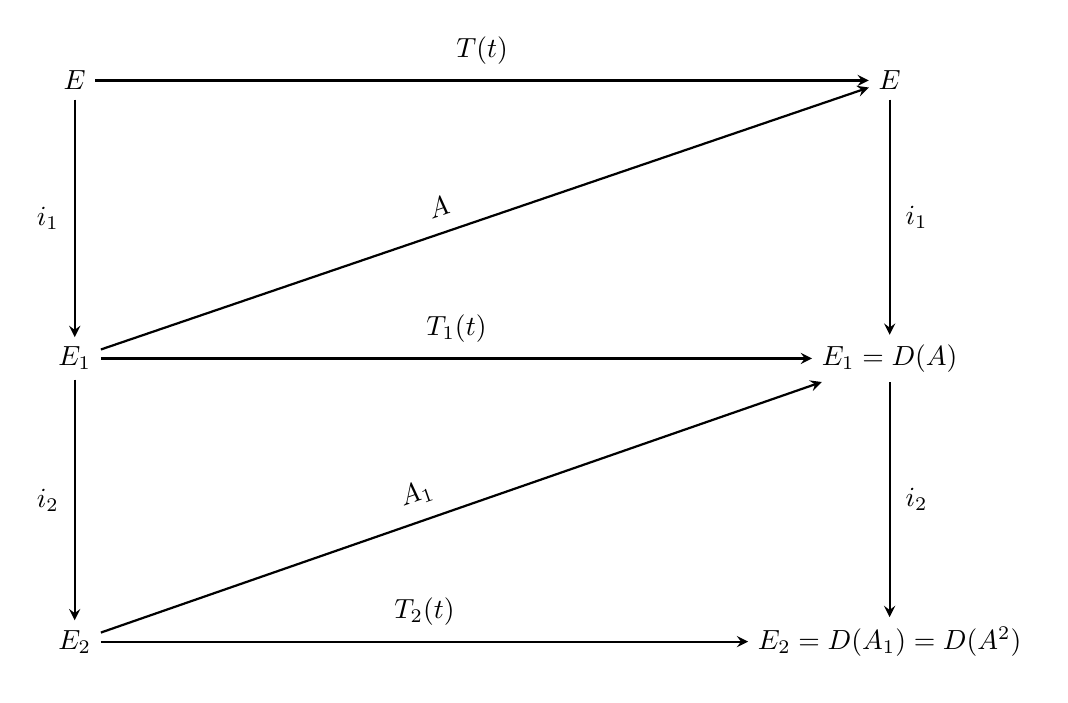
\begin{tikzpicture}[
    >=stealth,
    node distance=2.5cm,
    every node/.style={transform shape},
    label distance=3mm
]
    % Matrix mit verbessertem Spacing und Ausrichtung
    \matrix (m) [
        matrix of math nodes,
        row sep=3cm,    
        column sep=4cm, 
        nodes={anchor=center},
        nodes in empty cells
    ] {
        E & & E \\
        E_{1} & & E_{1} = D(A) \\
        E_{2} & & E_{2} = D(A_{1}) = D(A^{2}) \\
    };
    % Horizontale Pfeile mit einheitlicher Positionierung
    \draw[thick,->] (m-1-1) -- node[above=2pt] {$T(t)$} (m-1-3);
    \draw[thick,->] (m-2-1) -- node[above=2pt] {$T_{1}(t)$} (m-2-3);
    \draw[thick,->] (m-3-1) -- node[above=2pt] {$T_{2}(t)$} (m-3-3);
    % Vertikale Pfeile mit einheitlicher Beschriftung
    \draw[thick,->] (m-1-1) -- node[left=2pt] {$i_{1}$} (m-2-1);
    \draw[thick,->] (m-2-1) -- node[left=2pt] {$i_{2}$} (m-3-1);
    \draw[thick,->] (m-1-3) -- node[right=2pt] {$i_{1}$} (m-2-3);
    \draw[thick,->] (m-2-3) -- node[right=2pt] {$i_{2}$} (m-3-3);
    % Diagonale Pfeile mit verbesserter Platzierung
    \draw[thick,->] (m-2-1) -- node[above=2pt, sloped, pos=0.45] {$A$} (m-1-3);
    \draw[thick,->] (m-3-1) -- node[above=2pt, sloped, pos=0.45] {$A_{1}$} (m-2-3);
    % Gleichheitszeichen mit verbessertem Abstand
%    \node at ($(m-2-3)+(1.5,0)$) {$=$};
%    \node at ($(m-3-3)+(1.5,0)$) {$=$};
%    \node at ($(m-3-5)+(1.5,0)$) {$=$};
\end{tikzpicture}
\end{center}
%% --
%\newpage
%\begin{center}
%\begin{tikzpicture}[scale=1.5]
%% Nodes
%\node (E1) at (0,6) {$E$};
%\node (E2) at (4,6) {$E$};
%\node (E11) at (0,4) {$E_1$};
%\node (E12) at (4,4) {$E_1 = D(A)$};
%\node (E21) at (0,2) {$E_2$};
%\node (E22) at (4,2) {$E_2 = D(A_1) = D(A^2)$};
%\node (E31) at (0,0) {$E_3$};
%\node (E32) at (4,0) {$E_3$};
%
%% Horizontal arrows
%\draw[->] (E1) -- node[above] {$T(t)$} (E2);
%\draw[->] (E11) -- node[above] {$T_1(t)$} (E12);
%\draw[->] (E21) -- (E22);
%\draw[->] (E31) -- (E32);
%
%% Vertical arrows up
%\draw[->] (E11) -- node[left] {$i_1$} (E1);
%\draw[->] (E21) -- node[left] {$i_2$} (E11);
%\draw[->] (E31) -- node[left] {$i_3$} (E21);
%
%% Vertical arrows right side
%\draw[->] (E12) -- node[right] {$i_1$} (E2);
%\draw[->] (E22) -- node[right] {$i_2$} (E12);
%\draw[->] (E32) -- node[right] {$i_3$} (E22);
%
%% Diagonal arrows A
%\draw[->] (E1) -- node[above right] {$A$} (E12);
%\draw[->] (E11) -- node[above right] {$A_1$} (E22);
%\draw[->] (E21) -- node[above right] {} (E32);  % Unlabeled diagonal arrow
%\end{tikzpicture}
%\end{center}
%\newpage
%% --
For the translation semigroup on $L^{p}(\R)$ (see 2.3) the above construction leads to the usual \emph{Sobolev spaces}.
Therefore we might call $E_{n}$ the \emph{n-th Sobolev space} and $(T_{n}(t))_{t \geq 0}$ the \emph{n-th Sobolev semigroup} associated to $E$ and $(T(t))_{t \geq 0}$.
%% --
\begin{remark}\label{rem:a1-19.1}
\index{Sobolev spaces}
\index{Semigroups!Sobolev}
For $\lambda \in \rho(A)$ the operator $(\lambda - A)$ and the resolvent $R(\lambda,A)$ are isomorphisms from $E_{1}$ onto $E$, \resp from $E$ onto $E_{1}$ (show that $\|\cdot\|_{1}$ and $\|\cdot\|_{\lambda}$ with $\|\cdot\|_{\lambda} \coloneqq \|(\lambda - A)\cdot\|$ are equivalent).
%% --
In addition, the following diagram commutes. 
%% --
%\begin{tikzpicture}
%\matrix (m) [matrix of math nodes, row sep=3em, column sep=4em]
%{
%    E & & E \\
%    E_{1} & & E_{1} \\
%};
%\path[-stealth]
%(m-1-1) edge node[above] {$T(t)$} (m-1-3)
%(m-2-1) edge node[above] {$T_{1}(t)$} (m-2-3)
%(m-1-1) edge node[left] {$\lambda-A$} (m-2-1)
%(m-1-3) edge node[right] {$R(\lambda,A)$} (m-2-3);
%\end{tikzpicture}
%% --
\begin{center}
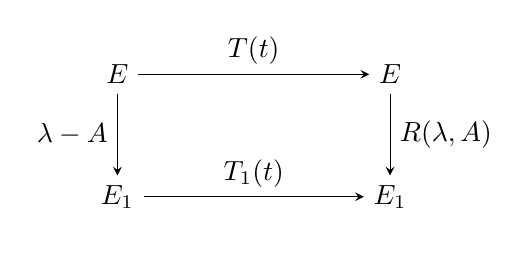
\begin{tikzpicture}[
    >=stealth,
    every node/.style={transform shape}
]
    % Matrix mit optimiertem Spacing
    \matrix (m) [
        matrix of math nodes,
        row sep=3em,    
        column sep=4em,
        nodes={anchor=center}
    ] {
        E    & & E \\
        E_{1}  & & E_{1} \\
    };
    % Pfeile als Pfad mit verbesserter Positionierung
    \path[->]
        (m-1-1) edge node[above] {$T(t)$} (m-1-3)
        (m-2-1) edge node[above] {$T_{1}(t)$} (m-2-3)
        (m-1-1) edge node[left] {$\lambda-A$} (m-2-1)
        (m-1-3) edge node[right] {$R(\lambda,A)$} (m-2-3);
    
\end{tikzpicture}
\end{center}
%% --
Therefore all Sobolev semigroups $(E_{n}, T_{n}(t))_{t \geq 0}$, $n \in \N$, are isomorphic.
\end{remark}
%% --
\begin{remark}\label{rem:a1-19.2}
For $\lambda \in \rho(A)$ consider the norm
%% --
\[
    \|f\|_{-1} \coloneqq \|R(\lambda,A)f\|
\]
%% --
for every $f \in E$ and define $E_{-1}$ as the completion of $E$ for $\|\cdot\|_{-1}$.
\end{remark}
%% --
Then $(T(t))_{t \geq 0}$ extends continuously to a strongly continuous semigroup $(T_{-1}(t))_{t \geq 0}$ on $E_{-1}$ and the above diagram can be extended to the negative integers.
%% --
\section{The \texorpdfstring{$\mathcal{F}$}{F}-Product Semigroup}\label{sec:a1-3.6}
\index{$\mathcal{F}$-Product}
\index{$\mathcal{F}$-Product!Semigroup}
%% --
It is standard in functional analysis to consider a sequence of points in a certain space as a point in a new and larger space.
In particular such a method can serve to convert an approximate eigenvector of a linear operator into an eigenvector.
Occasionally we will need such a construction and refer to Section V.1 of \citet{schaefer:1974}. 

If we try to adapt this construction to strongly continuous semigroups we encounter the difficulty that the semigroup extended to the larger space will not remain strongly continuous.
An idea already used in 3.4 will help to overcome this difficulty.

Let $\mathcal{T} = (T(t))_{t \geq 0}$ be a strongly continuous semigroup on the Banach space $E$.
Denote by $m(E)$ the Banach space of all bounded $E$-valued sequences endowed with the norm
%% --
\[
    \|(f_{n})_{n \in \N}\| \coloneqq \sup \{\|f_{n}\| \colon n \in \N\} .
\]
%% --
It is clear that every $T(t)$ extends canonically to a bounded linear operator
%% --
\[
    \hat{T}(t)(f_{n}) \coloneqq (T(t)f_{n})
\]
%% --
on $m(E)$, but the semigroup $(\hat{T}(t))_{t \geq 0}$ is strongly continuous if and only if $T$ has a bounded generator.
Therefore we restrict our attention to the closed, $(\hat{T}(t))$-invariant subspace
%% --
\[
    m^{\mathcal{T}}(E) \coloneqq \{(f_{n}) \in m(E) \colon \lim_{t \to 0} \|T(t)f_{n}-f_{n}\| = 0 \text{ uniformly for } n \in \N\} .
\]
%% --
Then the restricted semigroup
%% --
\[
    \hat{T}(t)(f_{n}) = (T(t)f_{n}), \quad (f_{n}) \in m^{\mathcal{T}}(E)
\]
%% --
is strongly continuous and we denote its generator by $(\hat{A},D(\hat{A}))$.

The following lemma shows that $\hat{A}$ is obtained canonically from $A$.
%% --
\begin{lemma}\label{lem:a1-3.6}
For the generator $\hat{A}$ of $(\hat{T}(t))_{t \geq 0}$ on $m^{\mathcal{T}}(E)$ one has the following properties.
%% --
\begin{enumerate}[(i)]

\item 
$D(\hat{A}) = \{(f_{n}) \in m^{\mathcal{T}}(E) \colon f_{n} \in D(A) \text{ and } (Af_{n}) \in m^{\mathcal{T}}(E)\}$,

\item 
$\hat{A}(f_{n}) = (Af_{n})$ for $(f_{n}) \in D(\hat{A})$ .
\end{enumerate}

\end{lemma}
%% --
For the proof we refer to Lemma 1.4. of \citet{derndinger:1980}.

Now let $\mathcal{F}$ be any filter on $\N$ finer than the Frechét filter (\ie the filter of sets with finite complement. In most cases $F$ will be either the Frechét filter or some free ultra filter.)
%% --
The space of all $\mathcal{F}$-null sequences in $m(E)$, \ie
%% --
\[
    c_{\mathcal{F}}(E) \coloneqq \{(f_{n}) \in m(E) \colon \mathcal{F}\text{-}\lim\|f_{n}\| = 0\}
\]
%% --
is closed in $m(E)$ and invariant under $(\hat{T}(t))_{t \geq 0}$. 
We call the quotient spaces
%% --
\[
    E_{\mathcal{F}} \coloneqq m(E)/c_{\mathcal{F}}(E) \quad \text{and} \quad E_{\mathcal{F}}^{T} \coloneqq m^{\mathcal{T}}(E)/c_{\mathcal{F}}(E)\cap m^{\mathcal{T}}(E)
\]
%% --
the \emph{$\mathcal{F}$-product of $E$} and the \emph{$ \mathcal{F} $-product of $E$ with respect to the semigroup $T$}, respectively.

Thus $E_{\mathcal{F}}^{T}$ can be considered as a closed linear subspace of $E_{\mathcal{F}}$. 
We have $E_{\mathcal{F}}^{T} = E_{\mathcal{F}}$ if (and only if) $T$ has a bounded generator.

The canonical quotient norm on $E_{\mathcal{F}}$ is given by
%% --
\[
    \|(f_{n}) + c_{\mathcal{F}}(E)\| = \mathcal{F}\text{-}\lim \sup \|f_{n}\| .
\]
%% --
We can apply Subsec.\;\ref{subsec:a1-3.3} in order to define the \emph{$\mathcal{F}$-product semigroup} $(T_{\mathcal{F}}(t))_{t \geq 0}$ on $E_{\mathcal{F}}^{T}$ by
%% --
\[
    T_{\mathcal{F}}(t)((f_{n}) + c_{\mathcal{F}}(E)) \coloneqq (T(t)f_{n}) 
    	+ c_{\mathcal{F}}(E)\cap m^{\mathcal{T}}(E)
\]
%% --
Thus $T_{\mathcal{F}}(t)$ is the restriction of $T(t)_{F}$ where $T(t)_{F}$ denotes the canonical extension of $T(t)$ to the $\mathcal{F}$-product $E_{\mathcal{F}}$. 
But note that $(T(t)_{F})_{t \geq 0}$ is not strongly continuous unless $T$ has a bounded generator.

With the canonical injection $j \colon f \mapsto (f,f,f,\ldots) + c_{\mathcal{F}}(E)$ from $E$ into $E_{\mathcal{F}}^{T}$ the operators $T_{\mathcal{F}}(t)$ are extensions of $T(t)$ satisfying $\|T_{\mathcal{F}}(t)\| = \|T(t)\|$. The basic facts about the generator $(A_{\mathcal{F}},D(A_{\mathcal{F}}))$ of $(T_{\mathcal{F}}(t))_{t \geq 0}$ follow from 3.3 and are collected in the following proposition.
%% --
\begin{proposition}\label{prop:a1-3.6}
For the generator $(A_{\mathcal{F}},D(A_{\mathcal{F}}))$ of the $\mathcal{F}$-product semigroup the following holds.
%% --
\begin{enumerate}[(i)]
\item 
$D(A_{\mathcal{F}}) = \{(f_{n}) + c_{\mathcal{F}}(E) \colon f_{n} \in D(A); (f_{n}), (Af_{n}) \in m^{\mathcal{T}}(E)\}$,

\item 
$A_{\mathcal{F}}((f_{n}) + c_{\mathcal{F}}(E)) = (Af_{n}) + c_{\mathcal{F}}(E)$.

\end{enumerate}
\end{proposition}
%% --
In case $A$ is a bounded operator then $D(A_{\mathcal{F}}) = E_{\mathcal{F}}^{T} = E_{\mathcal{F}}$ and $A_{\mathcal{F}}$ is the canonical extension of $A$ to $E_{\mathcal{F}}$.

We will show in A-III,4.5 that the above construction preserves and even improves many spectral properties of the semigroup and its generator.

%% --
\section{The Tensor Product Semigroup}\label{sec:a1-3.7}
\index{Tensor Product Semigroup}

%% --
Real- or complex-valued functions of two variables $x$, $y$ are often limits of functions of the form $\sum_{i=1}^{n} f_{i}(x)g_{i}(y)$ which, to some extent, allows one to consider the variables $x$ and $y$ separately.
Since algebraic manipulation with these latter functions is governed by the formal rules of a tensor product, it is customary to identify (for example) the function
%% --
\[
    (x,y) \mapsto f(x)g(y)
\]
%% --
with the tensor product $f \otimes g$ and to consider limits of linear combinations of such functions as elements of a completed tensor product.

To be more precise, we briefly present the most important examples for this situation.
%% --
\begin{examples}\label{ex:a1-5.1}
%% --
\begin{enumerate}[(i), wide, labelsep=1em, itemindent=\parindent]

\item
Let $(X,\Sigma,\mu)$ and $(Y,\Omega,\nu)$ be measure spaces. 
If we identify for $f_{i} \in L^{p}(\mu)$, $g_{i} \in L^{p}(\nu)$ the elements $\sum_{i=1}^{n} f_{i} \otimes g_{i}$ of the tensor product
%% --
\[
    L^{p}(\mu) \otimes L^{p}(\nu)
\]
%% --
with the (class of $\mu \times \nu$-a.e.-defined) functions
%% --
\[
    (x,y) \mapsto \sum_{i=1}^{n} f_{i}(x)g_{i}(y) ,
\]
%% --
then $L^{p}(\mu) \otimes L^{p}(\nu)$ becomes a dense subspace of $L^{p}(X\times Y,\Sigma\times\Omega,\mu\times\nu)$ for $1 \leq p < \infty$.

\item
Similarly, let $X$,$Y$ be compact spaces. Then $C(X) \otimes C(Y)$ becomes a dense subspace of $C(X\times Y)$ by identifying, for $f \in C(X)$ and $g \in C(Y)$, $f \otimes g$ with the function
%% --
\[
    (x,y) \mapsto f(x)g(y) .
\]
%% --
\end{enumerate}
\end{examples}
%% --
We do not intend to go deeper into the quite sophisticated problems related to normed tensor products of general Banach spaces, but will rather confine ourselves to the discussion of certain special cases.
These will always be related to one of the following standard methods to define a norm on the tensor product of two Banach spaces $E$, $F$.

Let $u \coloneqq \sum_{i=1}^{n} f_{i} \otimes g_{i}$ be an element of $E \otimes F$. 
Then
%% --
\begin{enumerate}[(i), wide, labelsep=1em, itemindent=\parindent]

\item
$\|u\|_{\pi} \coloneqq \inf\{\sum_{j=1}^{m} \|h_{j}\|\|k_{j}\| \colon u = \sum_{j=1}^{m}h_{j} \otimes k_{j}, h_{j} \in E, k_{j} \in F\}$ defines the \emph{greatest cross norm $\pi$} on $E \otimes F$.

\item
$\|u\|_{\epsilon} \coloneqq \sup\{\langle u,\phi \otimes \psi\rangle \colon \phi \in E', \psi \in F', \|\phi\|, \|\psi\| \leq 1\}$ defines the 
\emph{least cross norm $\epsilon$} on $E \times F$. 
Here, $\langle u,\phi \otimes \psi\rangle$ denotes the canonical bilinear form on $(E \otimes F) \times (E' \otimes F')$, \ie $\langle\sum_{i=1}^{n} f_{i} \otimes g_{i},\phi \otimes \psi\rangle = \sum_{i=1}^{n} \langle f_{i},\phi\rangle\langle g_{i},\psi\rangle$.

\item
if $E$ and $F$ are Hilbert spaces, $\|u\|_{h} = (u|u)_{h}^{1/2}$, where the scalar product $(\cdot|\cdot)_{h}$ is defined as in (ii), defines the \emph{Hilbert norm $h$} on $E \otimes F$.
\end{enumerate}
%% --
In the following we write $E \otimes_{\alpha} F$ for the tensor product of $E$ and $F$ endowed---if applicable---with one of the norms $\pi$, $\epsilon$, $h$ just defined.
In each case one has $\|f \otimes g\| = \|f\|\|g\|$ for $f \in E$, $g \in F$.

By $E \widetilde{\otimes}_{\alpha} F$ we mean the completion of $E \otimes_{\alpha} F$. 
Moreover we recall how examples (i) and (ii) above fit into this pattern
%% --
\[
    L^{1}(\mu \otimes \nu) = L^{1}(\mu) \widetilde{\otimes}_{\pi} L^{1}(\nu), 
    \quad L^{2}(\mu \otimes \nu) = L^{2}(\mu) \widetilde{\otimes}_{h} L^{2}(\nu),
\]
\[
    C(X \otimes Y) = C(X) \widetilde{\otimes}_{\epsilon} C(Y).
\]
%% --
Finally, we point out that for any $S \in \LE$, $T \in \L{F} $, the mapping
%% --
\[
    \sum_{i=1}^{n}f_{i} \otimes g_{i} \mapsto \sum_{i=1}^{n}Sf_{i} \otimes Tg_{i}
\]
%% --
defined on $E \otimes F$ is linear and continuous on $E \otimes_{\alpha} F$, hence has a continuous extension to $ E \widetilde{\otimes}_{\alpha} F$. 
This operator, as well as its continuous extension, will be denoted by $S \otimes T$ and satisfies $\|S \otimes T\| = \|S\|\|T\|$. 
The notation $A \otimes B$ will also be used in the obvious way if $A$ and $B$ are not necessarily bounded operators on $E$ and $F$. 
We are now ready to consider semigroups induced on the tensor product.
%% --
\begin{proposition}\label{prop:a1-3.7}
Let $(S(t))_{t\geq 0}$ and $(T(t))_{t\geq 0}$ be strongly continuous semigroups on Banach spaces $E$, $F$, and let $A$, $B$ be their generators. 
Then the family $(S(t) \otimes T(t))_{t\geq 0}$ is a strongly continuous semigroup on 
$ E \widetilde{\otimes}_{\alpha} F $.
The closure of $A \otimes \Id + \Id \otimes B$, defined on the core $D(A) \otimes D(B)$, is its generator.
\end{proposition}
%% --
\begin{proof}
It is immediately verified that $(S(t)\otimes T(t))_{t\geq 0}$ is in fact a semigroup of operators on 
$ E \widetilde{\otimes}_{\alpha} F $. 
The strong continuity need only be verified at $t = 0$ and on elements of the form $u = f \otimes g \in E \otimes F$.

This verification being straightforward, there remains to show that the generator of $(S(t)\otimes T(t))_{t\geq 0}$ is obtained as the closure of 
%
\[
	(A \otimes \Id + \Id \otimes B,D(A) \otimes D(B)) .
\]
%
To this end, let $f \in D(A)$ and $g \in D(B)$. 
Then
%% --
\begin{align*}
    &\lim_{h\to 0} \frac{1}{h}(T(h) \otimes S(h)(f \otimes g)-f \otimes g) \\
    &= \lim_{h\to 0} \frac{1}{h}(T(h)f \otimes (S(h)g-g) + (T(h)f-f) \otimes g) \\
    &= (f \otimes Bg) + (Af \otimes g) .
\end{align*}
%% --
Since the elements of the form $f \otimes g$, $f \in D(A)$, $g \in D(B)$, generate the linear subspace $D(A) \otimes D(B)$ of $E \otimes_{\alpha} F$, this subspace belongs
%% --
%\newpage
%% -- a1-25
to the domain of the generator.
Moreover, $D(A) \otimes D(B)$ is dense in $E \widetilde{\otimes}_{\alpha} F$ and invariant under $(S(t)\otimes T(t))_{t\geq 0}$, hence it is a core of $A \otimes \Id + \Id \otimes B$ by Prop.~\ref{prop:a1-1.9}\,(ii).
\end{proof}
%% --
\section{The Product of Commuting Semigroups}\label{sec:a1-3.8}
\index{Commuting Semigroups}
%% --
Let $(S(t))_{t\geq 0}$ and $(T(t))_{t\geq 0}$ be semigroups with generators $A$ and $B$, respectively on some Banach space $E$.
It is not difficult to see that the following assertions are equivalent.
%% --
\begin{enumerate}[(a), leftmargin=2em]

\item 
$S(t)T(t) = S(t)T(t)$ for all $t \geq 0$.

\item 
$R(\mu,A)R(\mu,B) = R(\mu,B)R(\mu,A)$ for some $\mu \in \rho(A) \cap \rho(B)$.

\item 
$R(\mu,A)R(\mu,B) = R(\mu,B)R(\mu,A)$ for all $\mu \in \rho(A) \cap \rho(B)$.

\end{enumerate}
%% --
In that case $U(t) = S(t)T(t)$ $(t \geq 0)$ defines a semigroup $(U(t))_{t\geq 0}$.
Using %Prop.~\ref{prop:a1-1.9}\,(ii).
Prop.~\ref{prop:a1-1.9}\,(ii) on p.~\pageref{prop:a1-1.9} 
one easily shows that $D_{0} \coloneqq D(A) \cap D(B)$ is a core for its generator $C$ and $Cf = Af + Bf$ for all $f \in D_{0}$.

\section*{Notes}
\addcontentsline{toc}{section}{Notes}
\index{Notes!Semigroup Theory}

For more complete information on semigroup theory we refer the reader to \citet{hillephillips:1957}, to the monographs by \citet{davies:1980}, 
\citet{goldstein:1985a} and \citet{pazy:1983}, to the survey article by \citet{kreinkhazan:1985}, to the bibliography by 
\citet{goldstein:1985b} and to \citet{engelnagel:2006}.

%% -- Literatur
%% --
\RaggedRight
\bibliographystyle{abbrvnat}
\bibliography{bib/ln-references} 

%% -- Chapter A-II
%% --

\chapter{Characterization of Semigroups on Banach Spaces}\label{chap:A-II}



% !TEX root = ../LN-Book.tex
%% --
%% -- Stand 2025-05-28 Final
%% --
\chapter{Spectral Theory}\label{chap:a3}%
%\index{Spectral Theory}
%% --
{\Large
\vspace*{-.75cm}
by \\[.25em]
Günther Greiner and Rainer Nagel 
\vspace{.75cm}
\\
}
%% --
\section{Introduction}%
%\index{Spectral Theory!Introduction}
%% --
In this chapter, we start a systematic analysis of the spectrum of a strongly continuous semigroup $\TT = (T(t))_{t\geq 0}$ on a complex Banach space $E$.
By the spectrum of the semigroup we understand the spectrum $\sigma(A)$ of the generator $A$ of $\TT$.
In particular, we are interested in the precise relations between $\sigma(A)$ and $\sigma(T(t))$.
The heuristic formula
%% --
\[
	T(t) = \mathrm{e}^{tA}
\]
%% --
serves as a leitmotiv and suggests relations of the form
%% --
\[
\sigma(T(t)) = \mathrm{e}^{t\sigma(A)} = \{ \mathrm{e}^{t\lambda} \colon \lambda \in \sigma(A) \} ,
\]
%% --
called \emph{spectral mapping theorem}.
These---or similar---relations will be of great use in Chapter IV and enable us to determine the asymptotic behavior of the semigroup $\TT$ by the spectrum of its generator.

As motivation and also as a preliminary step, we concentrate here on the \emph{spectral radius}
%% -- 
\begin{equation}\label{eq:a3-1.1}
	r(T(t)) := \sup \{ |\lambda| : \lambda \in \sigma(T(t)) \}, \quad t \geq 0 ,
\end{equation}
%% -- 
and show how it is related to the \emph{spectral bound}
%% -- 
\begin{equation}\label{eq:a3-1.2}
	s(A) := \sup \{ \Re\,\lambda : \lambda \in \sigma(A) \}
\end{equation}
%% -- 
of the generator $A$ and to the \emph{growth bound}
%% -- 
\begin{equation}\label{eq:a3-1.3}
	\omega_{0} := \inf \{\omega \in \R  : \|T(t)\| \leq M_{\omega}\cdot \mathrm{e}^{\omega t} \text{ for all } t \geq 0 \text{ and suitable } M_{\omega}\}
\end{equation}
%% -- 
of the semigroup $\TT = (T(t))_{t\geq 0}$.
(Recall that sometimes we write $\omega_{0}(\TT)$ or $\omega_{0}(A)$ instead of $\omega_{0}$).
%
The Examples~\ref{ex:a3-1.3} and \ref{ex:a3-1.4} below illustrate the main difficulties to be encountered.
%% -- Examples  1.3 and 1.4
\begin{proposition}\label{prop:a3-1.1}
Let $\omega_{0}$ be the growth bound of the strongly continuous semigroup $\TT = (T(t))_{t\geq 0}$.
Then
%% --
\begin{equation}\label{eq:a3-1.4}
	r(T(t)) = \mathrm{e}^{\omega_{0} t}
\end{equation}
%% --
for every $t \geq 0$.
\end{proposition}
%% --
\begin{proof}
From A-I, (1.1) we know that
%% --
\[
    \omega_{0}(\TT) = \lim_{t \to \infty} \frac{1}{t} \log \|T(t)\| .
\]
%% --
Since the spectral radius of $T(t)$ is given as
%% --
\[
    r(T(t)) = \lim_{n \to \infty} \|T(nt)\|^{1/n} ,
\]
%% --
we obtain for $t > 0$
%% --
\[
    r(T(t)) = \lim_{n \to \infty} \exp\left( \frac{t}{nt}\,\log \|T(nt)\|\right) = \mathrm{e}^{\omega_{0} t} .
\]
%% --
\end{proof}
%% --
It was shown in A-I, Proposition~1.11 that the spectral bound $s(A)$ is always dominated by the growth bound $\omega_{0}$ and therefore $\mathrm{e}^{s(A)t} \leq r(T(t))$.
If the above mentioned spectral mapping theorem holds---as is the case for bounded generators (\eg see Theorem~VII.3.11 of \citet{dunfordschwartz:1958})---we obtain the equality
%% --
\[
    \mathrm{e}^{s(A)t} = r(T(t)) = \mathrm{e}^{\omega_{0}(\TT) t} ,
\]
%% --
hence $s(A) = \omega_{0}(\TT)$.
Therefore, the following corollary is a consequence of the definitions of $s(A)$ and $\omega_{0}(\TT)$.
%% --
\begin{corollary}\label{cor:a3-1.2}
Consider the semigroup $\TT = (T(t))_{t \geq 0}$ generated by some bounded linear operator $A \in \L{E}$.
If $\Re\,\lambda < 0$ for each $\lambda \in \sigma(A)$, then $\lim_{t \to \infty}\|T(t)\| = 0$.
\end{corollary}
%% --
Through this corollary we have re-established a famous result of Liapunov which assures that the solutions of the linear Cauchy problem
%% --
\[
    \dot{x}(t) = Ax(t), \quad x(0) = x_{0} \in \C^{n} \quad \text{and} \quad A = (a_{ij})_{n\times n}
\]
%% --
are \emph{stable}, \ie they converge to zero as $t \to \infty$ if (and only if) the real parts of all eigenvalues of the matrix $A$ are smaller than zero.

For unbounded generators the situation is much more difficult and $s(A)$ may differ drastically from $\omega_{0}(\TT)$.
%% --
\begin{example}\label{ex:a3-1.3}(Banach function space, \citet{greinervoigtwolff:1981})
%% --
Consider the Banach space $E$ of all complex valued continuous functions on $\R_{+}$ which vanish at infinity and are integrable for $\mathrm{e}^{x}\dx$, \ie 
%% --
\[
    E \coloneqq C_{0}(\R_{+}) \cap L^{1}(\R_{+}, \mathrm{e}^{x}\dx)
\]
%% --
endowed with the norm
%% --
\[
    \|f\| \coloneqq \|f\|_{\infty} + \|f\|_{1} = \sup\{|f(x)| \colon x \in \R_{+}\} + \int_{0}^{\infty} |f(x)|\mathrm{e}^{x} \dx .
\]
%% --
\end{example}
%% --
The translation semigroup
%% --
\[
    T(t)f(x) \coloneqq f(x+t)
\]
%% --
is strongly continuous on $E$ and one shows as in A-I, 2.4 that its generator is given by
%% --
\[
    Af = f', \quad D(A) = \{ f \in E \colon f \in C^{1}(\R_{+}), f' \in E \} .
\]
%% --
First we observe that $\|T(t)\| = 1$ for every $t \geq 0$, hence $\omega_{0}(\TT) = 0$.
Moreover it is clear that $\lambda$ is an eigenvalue of $A$ as soon as $\Re\,\lambda < -1$ (in fact: the function
%% --
\[
    x \mapsto e_{\lambda}(x) \coloneqq \mathrm{e}^{\lambda x}
\]
%% --
belongs to $D(A)$ and is an eigenvector of $A$), hence $s(A) \geq -1$.
For $f \in E$ and $\Re \, \lambda > -1$ 
%% --
\[
    \|\cdot\|_{1}\text{-}\lim_{t \to \infty} \int_{0}^{t} \mathrm{e}^{-\lambda s}T(s)f \, \ds
\]
%% --
exists since $\|T(s)f\|_{1} \leq \mathrm{e}^{-s}\|f\|_{1}$ for $s \geq 0$, and
%% --
\[
    \|\cdot\|_{\infty}\text{-}\lim_{t \to \infty} \int_{0}^{t} \mathrm{e}^{-\lambda s}T(s)f \, \ds
\]
%% --
exists since $\int_{0}^{\infty} \mathrm{e}^{x}|f(x)| \, \dx < \infty$.
Therefore $\int_{0}^{\infty} \mathrm{e}^{-\lambda s}T(s)f \, \ds$ exists in $E$ for every $f \in E$, $\Re\,\lambda > -1$.

As we observed in A-I, Proposition~1.11, this implies $\lambda \in \rho(A)$.
Therefore $\TT = (T(t))_{t\geq 0}$ is a semigroup having $s(A) = -1$, but $\omega_{0}(\TT) = 0$.
%% --
\begin{example}\label{ex:a3-1.4}(Hilbert space, \citet{zabczyk:1975})
%% --
For every $n \in \N$ consider the $n$-dimensional Hilbert space $H_{n} \coloneqq \C^{n}$ and operators $A_{n} \in \mathcal{L}(H_{n})$ defined by the matrices
%% --
\[
    A_{n} =
    \begin{pmatrix}
    0 & 1 & \cdots & 0 \\
    \cdot & 0 & 1 & \cdot \\
    \cdot & \cdot & \cdot & 1 \\
    0 & \cdot & \cdot & 0
    \end{pmatrix}_{n \times n} .
\]
%% --
These matrices are nilpotent and therefore $\sigma(A_{n}) = \{0\}$.
The elements 
%% --
\[
	x_{n} \coloneqq n^{-1/2}(1, \ldots, 1) \in H_{n}
\]
%% --
satisfy the following properties.
%% --
\begin{enumerate}[\upshape (i)]
\item
	$\|x_{n}\| = 1$ for every $n \in \N$ , 

\item
	$\lim_{n \to \infty} \|A_{n}x_{n} - x_{n}\| = 0$ , 

\item
	$\lim_{n \to \infty} \|\exp(tA_{n})x_{n} - \mathrm{e}^{t}x_{n}\| = 0$. 

\end{enumerate}
%% --
Consider now the Hilbert space 
%
\[
	\text{$H \coloneqq \bigoplus_{n \in \N} H_{n}$ and the operator 
		$A \coloneqq (A_{n} + 2\pi\im n)_{n \in \N}$}
\]
%
with maximal domain in $H$.

Analogously we define a semigroup $\TT = (T(t))_{t \geq 0}$ by
%% --
\[
    T(t) \coloneqq (\mathrm{e}^{2\pi\im nt}\exp(tA_{n}))_{n \in \N} .
\]
%% --
\end{example}
%% --
Since $\|\exp(tA_{n})\| \leq \mathrm{e}^{t}$ for every $n \in \N$, $t \geq 0$, and since $t \mapsto T(t)x$ is continuous on each component $E_{n}$, it follows that $\TT$ is strongly continuous.
Its generator is the operator $A$ as defined above.

For $\lambda \in \C$, $\Re\,\lambda > 0$, we have 
$\lim_{n \to \infty} \|R(\lambda-2\pi\im n,A_{n})\| = 0$, hence
%% --
\[
    (R(\lambda,A_{n}+2\pi\im n))_{n \in \N} = (R(\lambda-2\pi\im n,A_{n}))_{n \in \N}
\]
%% --
is a bounded operator on $H$ representing the resolvent $R(\lambda,A)$.
Therefore we obtain $s(A) \leq 0$.
On the other hand, each $2\pi\im n$ is an eigenvalue of $A$, hence $s(A) = 0$.

Take now $x_{n} \in H_{n}$ as above and consider the sequence $(x_{n})_{n \in \N}$.
From (iii) it follows that for $t > 0$ the number $\mathrm{e}^{t}$ is an approximate eigenvalue of $T(t)$ with approximate eigenvector $(x_{n})_{n \in \N}$ (see Definition~\ref{def:a3-2.1} below).
Therefore 
%
\[
	 \mathrm{e}^{t} \leq r(T(t)) \leq \|T(t)\|
\]
%
and hence $\omega_{0}(\TT) \geq 1$.
On the other hand, it is easy to see that $\|T(t)\| = \mathrm{e}^{t}$, hence $\omega_{0}(\TT) = 1$.


Finally, if we take $S(t) \coloneqq \mathrm{e}^{-t/2}T(t)$, we obtain a semigroup $\mathcal{S}$ 
having spectral bound $-\frac{1}{2}$ but satisfying $\lim_{t \to \infty} \|S(t)\| = \infty$ in contrast with Corollary~\ref{cor:a3-1.2}.

These examples show that neither the conclusion of Corollary~\ref{cor:a3-1.2}, \ie \enquote{$s(A) < 0$ implies stability}, nor the \enquote{spectral mapping theorem}
%% --
\[
    \sigma(T(t)) = \exp(t\cdot\sigma(A))
\]
%% --
is valid for arbitrary strongly continuous semigroups.
A careful analysis of the general situation will be given in Section 6 below, but we will first develop systematically the necessary spectral theoretic tools for unbounded operators.
%% --
\section{The Fine Structure of the Spectrum}\label{sec:a3-2}%
%\index{Spectral Theory!Fine Structure of the spectrum}
%% --
As usual, to a closed linear operator $A$ with dense domain $D(A)$ in a Banach space $E$, we associate its spectrum $\sigma(A)$, its resolvent set $\rho(A)$ and its resolvent
%% --
\[
    \lambda \mapsto R(\lambda,A) \coloneqq (\lambda - A)^{-1}
\]
%% --
which is a holomorphic map from $\rho(A)$ into $\mathcal{L}(E)$.
In contrast to the finite dimensional situation, where a linear operator fails to be surjective if and only if it fails to be injective, we now have to distinguish different cases of \emph{non-invertibility} of $\lambda - A$.
This distinction gives rise to a subdivision of $\sigma(A)$ into different subsets.
We point out that these subsets need not be disjoint. Our definitions are
justified by the fact that for each of the following subsets of $\sigma(A)$ there exist canonical constructions converting the corresponding spectral values into eigenvalues (see Proposition~\ref{prop:a3-2.2}.(ii) and Proposition~\ref{prop:a3-4.4} below).
%% --
\begin{definition}\label{def:a3-2.1}
For a closed, densely defined, linear operator $A$ with domain $D(A)$ in the Banach space $E$ denote by the
%% --
\begin{enumerate}[\upshape (i)]
\item 
\emph{point spectrum} $P\sigma(A)$ the set of all $\lambda \in \C$ such that 
$A - \lambda$ is not injective.

\item 
\emph{approximate point spectrum} $A\sigma(A)$ the set of all $\lambda \in \C$ such that $A - \lambda$ is not injective or $(A - \lambda)D(A)$ is not closed in $E$ .

\item 
\emph{residual spectrum} $R\sigma(A)$ the set of all $\lambda \in \C$ such that $(A - \lambda)D(A)$ is not dense in $E$.
\end{enumerate}
\end{definition}
%% --
From these definitions it follows that $\lambda \in P\sigma(A)$ if and only if there exists a non-zero \emph{eigenvector} $f \in D(A)$ such that $Af = \lambda f$, \ie $\lambda$ is an \emph{eigenvalue}.
%% --
It follows from the \emph{Open Mapping Theorem} that $\lambda \in A\sigma(A)$ if and only if $\lambda$ is an \emph{approximate eigenvalue}, \ie there exists a sequence $(f_{n})_{n \in \N} \subset D(A)$, called an\emph{ approximate eigenvector}, such that $\|f_{n}\| = 1$ and $ \lim_{n \to \infty} \|Af_{n} - \lambda f_{n}\| = 0$.

Clearly we have $P\sigma(A) \subset A\sigma(A)$ and $\sigma(A) = A\sigma(A) \cup R\sigma(A)$ where the union need not be disjoint.

The following proposition is a first indication that the subdivision we made yields nice properties.
%% --
\begin{proposition}\label{prop:a3-2.2}
%% --
For a closed, densely defined, linear operator $(A,D(A))$ in a Banach space $E$ the following holds.
%% --
\begin{enumerate}[\upshape (i)]

\item
The topological boundary $\partial\sigma(A)$ of $\sigma(A)$ is contained in $A\sigma(A)$.

\item
$R\sigma(A) = P\sigma(A')$ for the adjoint operator $A'$ on $E'$.

\end{enumerate}
\end{proposition}
%% --
\begin{proof}
\begin{enumerate}[\upshape (i), wide, labelindent=.5em]

\item 
Take $\lambda_{0} \in \partial\sigma(A)$ and $\lambda_{n} \in \rho(A)$ such that $\lambda_{n} \to \lambda_{0}$.
Since 
%
\[
	 \|R(\lambda_{n},A)\| \geq r(R(\lambda_{n},A)) = (\text{dist}(x,\sigma(A)))^{-1} 
\]
%
(see Proposition~\ref{prop:a3-2.5}.(ii)), by the uniform boundedness principle we find $f \in E$ such that
%% --
\[
	\lim_{n \to \infty}\|R(\lambda_n ,A)f\| = \infty .
\]
%% --
Define $g_{n} \in D(A)$ by
%% --
\[
g_{n} \coloneqq \|R(\lambda_{n},A)f\|^{-1} R(\lambda_{n},A)f
\]
%% --
and use the identity
%% --
\[
	(\lambda_{0} - A)g_{n} = (\lambda_{0} - \lambda_{n})g_{n} + (\lambda_{n} - A)g_{n}
\]
%% --
to show that $(g_{n})_{n \in \N}$ is an approximate eigenvector corresponding to $\lambda_{0}$.

\item 
This is a simple consequence of the Hahn-Banach theorem.
%% --
\end{enumerate}
\end{proof}
%% --
In order to illuminate the above definitions we now return to the Standard Examples introduced in Section 2 of A-I and discuss the fine structure of the spectrum of these strongly continuous semigroups, \ie of their generators and their semigroup operators.
%% --
\begin{example}{(The Spectrum of Multiplication Semigroups)}\label{ex:a3-2.3}%
%\index{Spectral Theory!Example!Multiplication Semigroups}
%% --
Take $E = C_{0}(X)$ for some locally compact space $X$ and take a continuous function $q \colon X \mapsto \C$ whose real part is bounded above.
As observed in A-I,2.3 the multiplication operator
%% --
\[
M_{q} \colon f \mapsto q \cdot f
\]
%% --
with maximal domain $D(M_{q})$ generates the multiplication semigroup
%% --
\[
T(t)f \coloneqq \mathrm{e}^{tq} \cdot f \, , \, f \in E .
\]
%% --
Since $M_{q}$ is bounded if and only if $q$ is bounded, we conclude that $M_{q}$ is invertible (with bounded inverse $M_{1/q}$) if and only if
%% --
\[
0 \notin \overline{\{q(x)  \colon x \in X\}} .
\]
%% --
Therefore we obtain
%% --
\[
\sigma(M_{q}) = \overline{q(X)} = \overline{\{q(x) \colon x \in X\}} ,
\]
%% --
and
%% --
\[
\sigma(T(t)) = \overline{\{\exp(tq(x)) \colon x \in X\}} .
\]
%% --
In particular the following \emph{weak spectral mapping theorem} is valid
%% --
\[
\sigma(T(t)) = \overline{\exp(t\sigma(M_{q}))} .
\]
%% --
In addition, we observe that to each spectral value of $A$ (\resp of $T(t)$) there exists an approximate eigenvector and hence
%% --
\[
\sigma(A) = A\sigma(A) \text{ and } \sigma(T(t)) = A\sigma(T(t)) .
\]
%% --
Since each Dirac functional is an eigenvector for the adjoint multiplication operator, we obtain
%% --
\[
q(X) \subset R\sigma(M_{q}) \text{ and } \mathrm{e}^{tq(X)} \subset R\sigma(T(t)) .
\]
%% --
The eigenvalues of $M_{q}$ can be characterized as follows.
%% --
\begin{quote}
$\lambda \in P\sigma(M_{q})$ if and only if the set $\{x \in X \colon q(x) = \lambda\}$ has non empty interior (analogously for $P\sigma(T(t))$).
\end{quote}
%% --
For example, it follows that $P\sigma(M_{q}) = \emptyset$ for $E = C_{0}(\R_{+})$ and $q(x) = -x$, $x \in \R_{+}$.

On $E = L^{p}(X,\Sigma,\mu)$ analogous results are valid, but their exact formulation---using the notion \emph{essential range}, see \citet{goldstein:1985a}---is left to the reader.
%% --
\end{example}
%% --
\begin{example}{(The Spectrum of Translation Semigroups)}\label{ex:a3-2.4}%
%\index{Spectral Theory!Example!Translation Semigroups}
%% --
We consider the translation semigroup
%% --
\[
T(t)f(x) \coloneqq f(x+t)
\]
%% --
on $E = C_{0}(\R_{+})$ (or $L^{p}(\R_{+})$, see A-I,2.4).
Its generator $A$ is the first derivative and for every $\lambda \in \C$, $\Re\,\lambda < 0$, the function $\epsilon_{\lambda} \colon x \mapsto \mathrm{e}^{\lambda x}$ belongs to $D(A)$ and satisfies
%% --
\[
A\epsilon_{\lambda} = \lambda\epsilon_{\lambda} ,
\]
%% --
hence $\lambda \in P\sigma(A)$.

Since $\TT = (T(t))_{t \geq 0}$ is a contraction semigroup it follows that 
%
\[
	 \text{$\sigma(A) = \{\lambda \in \C \colon \Re\lambda \leq 0\}$  and $\im\R \subset A\sigma(A)$}  
\]
%
(use Proposition~\ref{prop:a3-2.2}.(i)) or show directly that $f_{n}(x) = \mathrm{e}^{ \im\alpha x}\mathrm{e}^{-x/n}$ defines an approximate eigenvector for $\im\alpha$, $\alpha \in \R$).
Using the same functions one obtains
%% --
\begin{align*}
	P\sigma(T(t)) &= \{\mathrm{e}^{\lambda t} \colon \Re\,\lambda < 0\} = \{z \in \C \colon |z| < 1\} ,\\
	\sigma(T(t)) &= \{z \in \C \colon |z| \leq 1\} \text{ for every } t > 0 .
\end{align*}
%% --
In the case of the translation group on $E = C_{0}(\R)$ one has $\sigma(A) \subset \im\R$.
As above one obtains approximate eigenvectors for every $\alpha \in \R$ from 
$f_{n}(x) = \mathrm{e}^{\im\alpha x}\mathrm{e}^{-|x|/n}$, hence
%% --
\[
\sigma(A) = A\sigma(A) = \im\R .
\]
%% --
The generator $A$ of the nilpotent translation semigroup A-I,2.6 has empty spectrum by A-I, Proposition~1.11.
The resolvent is given by
%% --
\[
R(\lambda,A)f(x) = \mathrm{e}^{\lambda x}\int_{x}^{\infty}\mathrm{e}^{-\lambda s}f(s)  \ds \quad (f \in L^{p}([0,\tau]), \lambda \in \C) .
\]
%% --
Finally, the generator of the periodic translation group from A-I,2.5 on
%% --
\[
	E = \{f \in C[0,1] \colon f(0) = f(1)\}
\]
%
has point spectrum
%% --
\[
P\sigma(A) = 2\pi \im\Z
\]
%% --
with eigenfunctions $\epsilon_{n}(x) \coloneqq \exp(2\pi \im n x)$.
In Section 5 we show that $\sigma(A) = 2\pi \im\Z$.
%% --
\end{example}
%% --
We now return to the general theory and recall from Corollary~\ref{cor:a3-1.2} that it is very useful (\eg for stability theory) to be able to convert
spectral values of the generator $A$ into spectral values of the semigroup operator $T(t)$ and vice versa.
As shown in Examples~\ref{eq:a3-1.3} and \ref{eq:a3-1.4} this is not possible in general.
Therefore we tackle first a much easier \emph{spectral mapping theorem}: the relation between $\sigma(A)$ and $\sigma(R(\lambda_{0}))$, where $R(\lambda_{0}) \coloneqq R(\lambda_{0},A)$ for some $\lambda_{0} \in \rho(A)$.
%% --
\begin{proposition}\label{prop:a3-2.5}
Let $(A,D(A))$ be a densely defined closed linear operator with non-empty resolvent set $\rho(A)$.
For each $\lambda_{0} \in \rho(A)$ the following assertions hold.

\begin{enumerate}[\upshape (i)]
\item 
$\sigma(R(\lambda_{0})) \setminus \{0\} = (\lambda_{0} - \sigma(A))^{-1}$, in  particular, $r(R(\lambda_{0})) = (\mathrm{dist}(\lambda_{0},\sigma(A)))^{-1}$.

\item 
Analogous statements hold for the point-, approximate point-, residual spectra of $A$ and $R(\lambda_{0},A)$.

\item 
The point $\alpha$ is isolated in $\sigma(A)$ if and only if $(\lambda_{0}-\alpha)^{-1}$ is isolated in $\sigma(R(\lambda_{0}))$.
In that case the residues (\resp the pole orders) in $\alpha$ and in $(\lambda_{0}-\alpha)^{-1}$ coincide.
\end{enumerate}
\end{proposition}
%% --
\begin{proof}
\begin{enumerate}[\upshape (i), wide, labelindent=.5em]
\item 
is well known. It can be found for example in \citet[VII.9.2]{dunfordschwartz:1958}.

\item 
We show that $\alpha \in A\sigma(A)$ if $(\lambda_{0}-\alpha)^{-1} \in A\sigma(R(\lambda_{0}))$ and leave the proof of the remaining statements to the reader.

Take $(f_{n})_{n \in \N} \subset E$ such that $\|f_{n}\| = 1$, $\|(\lambda_{0}-\alpha)^{-1}f_{n} - R(\lambda_{0},A)f_{n}\| \to 0$ and $\|R(\lambda_{0},A)f_{n}\| \geq \frac{1}{2}|\lambda_{0} - \alpha|^{-1}$.
Define
%% --
\[
g_{n} \coloneqq \|R(\lambda_{0},A)f_{n}\|^{-1}R(\lambda_{0},A)f_{n} \in D(A)
\]
%% --
and deduce from
%% --
\begin{align*}
(\alpha-A)g_{n} &= \|R(\lambda_{0},A)f_{n}\|^{-1} \cdot 
		[(\lambda_{0}-A) - (\lambda_{0}-\alpha)]R(\lambda_{0},A)f_{n} \\  
	&= \|R(\lambda_{0},A)f_{n}\|^{-1} \cdot 			(\lambda_{0}-\alpha)[(\lambda_{0}-\alpha)^{-1} - R(\lambda_{0},A)]f_{n}
\end{align*}
%% --
that $(g_{n})$ is an approximate eigenvector of $A$ to the eigenvalue $\alpha$.

\item 
First we recall the wellknown \emph{resolvent equation}. For any $z$,  $\lambda_{0} \in \rho(A)$ we have $R(\lambda_{0},A) - R(z,A)= -(\lambda_{0}-z)R(\lambda_{0},A)R(z,A))$ . From this it follows that 
%
\[
	(\lambda_{0}-z)^2\cdot R(z,A) = \left((\lambda_{0}-z)^{-1}-R(\lambda_{0},A)\right)^{-1} - (\lambda_{0}-z).
\]
%
If we now take a circle $\Gamma$ with center $\alpha$ and sufficiently small radius, then the residue $P$ of $R(\cdot,A)$ at $\alpha$ is
%% --
\begin{align*}
P &=  \frac{1}{2\pi\im } \int_{\Gamma} R(z,A)   \diff{z} = \\
&=  \frac{1}{2\pi\im } \left[\int_{\Gamma} (\lambda_{0}-z)^{-2}R((\lambda_{0}-z)^{-1}\,R(\lambda_{0},A))  \diff{z}   - 
   \int_{\Gamma}(\lambda_{0}-z)^{-1} \diff{z} \right] . 
\end{align*}
%% --
If $\lambda_{0}$ lies in the exterior of $\Gamma$, the second integral is zero.
The substitution 
%
\[
	 \tilde{z} \coloneqq (\lambda_{0} - \tilde{z})^{-1} 
\]
%
yields a path $\tilde{\Gamma}$ around $(\lambda_{0}-\alpha)^{-1}$ and we obtain
%% --
\[
P = \frac{1}{2\pi\im } \int_{\tilde{\Gamma}} R(\tilde{z},R(\lambda_{0},A)) \, \mathrm{d}\tilde{z}
\]
%% --
which is the residue of $R(\cdot,R(\lambda_{0},A))$ at $(\lambda_{0}-\alpha)^{-1}$.
The final assertion on the pole order follows from the identities
%% --
\[
V_{-n} = ((\lambda_{0}-\alpha)^{-1}R(\lambda_{0},A))^{n-1}U_{-n} \quad (n \in \N) ,
\]
%% --
where $U_{n}$, \resp $V_{n}$ stand for the $ n $-th coefficient in the Laurent series of $R(\cdot,A)$, \resp $R(\cdot,R(\lambda_{0},A))$ at $\alpha$, \resp $(\lambda_{0}-\alpha)^{-1}$.
This has already been proved for $n = 1$ and follows for $n > 1$ by induction using the relations
%% --
\[
U_{-n-1} = (A - \alpha)U_{-n} 
\quad \text{and} \quad 
V_{-n-1} = \left(R(\lambda_{0},A) - (\lambda_{0}-\alpha)^{-1}\right)V_{-n} .
\]
\end{enumerate}
%% --
\end{proof}
%% --
\section{Spectral Decomposition}\label{sec:a3-3}%
%\index{Spectral Theory!Spectral Decomposition}
%% --
In the next two sections we develop some important techniques for our further investigation of semigroups and their generators.
Even though these methods are well known (compare, \eg Section VII.3 of \citet{dunfordschwartz:1958}) or rather technical, it is useful to present them in a coherent way.

Our interest in this section is the following: Let $E$ be a Banach space and $\TT = (T(t))_{t \geq 0}$ a strongly continuous semigroup with generator $A$.
Suppose that the spectrum $\sigma(A)$ splits into the disjoint union of two closed subsets $\sigma_{1}$ and $\sigma_{2}$.
Does there exist a corresponding decomposition of the space $E$ and the semigroup $\TT$\,?

In the following definition, we explain what we understand by \enquote{corresponding decomposition}.

\phantom{x}
%% --
\begin{definition}\label{def:a3-3.1}
Assume that $\sigma(A)$ is the disjoint union
%% --
\[
\sigma(A) = \sigma_{1} \cup \sigma_{2}
\]
%% --
of two non-empty closed subsets $\sigma_{1}$, $\sigma_{2}$.
A decomposition
%% --
\[
E = E_{1} \oplus E_{2}
\]
%% --
of $E$ into the direct sum of two non-trivial closed $\TT$-invariant subspaces is called a \emph{spectral decomposition} corresponding to $\sigma_{1} \cup \sigma_{2}$ if the spectrum $\sigma(A_{i})$ of the generator $A_{i}$ of $\TT_{i} \coloneqq (T(t)_{|E_{i}})_{t \geq 0}$ coincides with $\sigma_{i}$ for $i = 1$, $2$.
\end{definition}
%% --
For a better understanding of the above definition we recall that to every direct sum decomposition $E = E_{1} \oplus E_{2}$ there corresponds a continuous projection $P \in \LE$ such that $PE = E_{1}$ and $P^{-1}(0) = E_{2}$.
Moreover, the subspaces $E_{1}$, $E_{2}$ are $\TT$-invariant if and only if $P$ commutes with the semigroup $\TT$, \ie $T(t)P = PT(t)$ for every $t \geq 0$.
In this case it follows that the domain $D(A)$ of the generator $A$ splits analogously and $D(A) \cap E_{i}$ is the domain $D(A_{i})$ of the generator $A_{i}$ of the restricted semigroup $\TT_{i}$, $i = 1$, $2$.
We write
%% --
\[
A = A_{1} \oplus A_{2} .
\]
%% --
and say that \emph{$A$ commutes with $P$} and call $P$ a \emph{spectral projection}.
In terms of the generator $A$ this means that for $f \in D(A)$ we have $Pf \in D(A)$ and $APf = PAf$.

The existence of such projections reduces the semigroup $\TT$ into two (possibly simpler) semigroups $\TT_{1}$, $\TT_{2}$ such that
%% --
\[
\sigma(A) = \sigma(A_{1}) \cup \sigma(A_{2}) \quad \text{and} \quad \sigma(T(t)) = \sigma(T_{1}(t)) \cup \sigma(T_{2}(t)) .
\]
%% --
For example, in some cases (see Theorem~\ref{thm:a3-3.3} below) it can be shown that one of the reduced semigroups has additional properties.

In order to achieve such decompositions we will assume that $\sigma(A)$ decomposes into sets $\sigma_{1}$ and $\sigma_{2}$ and will then try to find a corresponding spectral projection.
Unfortunately such spectral decompositions do not exist in general.
%% --
\begin{example}\label{ex:a3-3.2}
%% --
Take the rotation semigroup from A-I,2.4 on the Banach space $L^{p}(\Gamma)$, $1 \leq p < \infty$, $\tau = 2\pi$.
It was stated in Example~\ref{ex:a3-2.4} and will be proved in Section 5 that its generator $A$ has spectrum
%% --
\[
\sigma(A) = P\sigma(A) = \im\Z
\]
%% --
where $\epsilon_{k}(z) \coloneqq z^{k}$ spans the eigenspace corresponding to $\im k$, $k \in \Z$.

Now, $\sigma(A)$ is the disjoint union of 
$\sigma_{1} \coloneqq \{0,\im ,2\im, \ldots\}$ 
and $\sigma_{2} \coloneqq \{-\im, -2\im, \ldots\}$.
By a result of M. Riesz there is no projection $P \in \L{L^{1}(\Gamma)}$ satisfying $P\epsilon_{k} = \epsilon_{k}$ for $k \geq 0$, $P\epsilon_{k} = 0$ for $k < 0$ , hence there is no spectral decomposition of $L^{1}(\Gamma)$ corresponding to $\sigma_{1}$, $\sigma_{2}$ (\citet[p.165]{lindenstraustzafriri:1979}).

On the other hand, for $L^{p}(\Gamma)$, $1 < p < \infty$, such a spectral projection exists (l.c., 2.c.15).
As long as $p \neq 2$ we can always decompose $\sigma(A)$ into suitable subsets admitting no spectral decomposition (l.c., remark before 2.c.15).
Clearly, for $p = 2$ such spectral decompositions always exist.
\end{example}
%% --
In the above example both subsets $\sigma_{1}$, $\sigma_{2}$ of $\sigma(A)$ are unbounded.
But as soon as one of these sets is bounded a corresponding spectral decomposition can always be found.
%% --
\begin{theorem}\label{thm:a3-3.3}
Let $\TT$ be a strongly continuous semigroup on a Banach space $E$ and assume that the spectrum $\sigma(A)$ of the generator $A$ can be decomposed into the disjoint union of two non-empty closed subsets $\sigma_{1}$ and 
$\sigma_{2}$.

If $\sigma_{1}$ is compact, then there exists a unique corresponding spectral decomposition $E = E_{1} \oplus E_{2}$ such that the restricted semigroup $\TT_{1}$ has a bounded generator.
\end{theorem}
%% --
\begin{proof}
We assume the reader to be familiar with the spectral decomposition theorem for bounded operators (see, \eg \citet[p.572]{dunfordschwartz:1958}) and apply the spectral mapping theorem for the resolvent (Proposition~\ref{prop:a3-2.5}.(i)) in order to decompose $R(\lambda,A)$ instead of $A$.

For $\lambda_{0} > \omega_{0}(\TT)$ it follows from Proposition~\ref{prop:a3-2.5} that $\sigma(R(\lambda_{0},A)) \setminus \{0\} = (\lambda_{0} - \sigma(A))^{-1}$.
From $\sigma(A) = \sigma_{1} \cup \sigma_{2}$ we obtain a decomposition of $\sigma(R(\lambda_{0},A)) \setminus \{0\}$ into
%% --
\[
	\tau_{1} \coloneqq (\lambda_{0} \setminus \sigma_{1})^{-1}, 
		\quad 
	\tau_{2} \coloneqq (\lambda_{0} \setminus \sigma_{2})^{-1} .
\]
%% --
Since $\sigma_{1}$ is compact, the set $\tau_{1}$ is compact and does not contain $0$.
Only in the case that $\sigma_{2}$ is unbounded, the point $0$ will be an accumulation point of $\tau_{2}$.
Therefore $\sigma(R(\lambda_{0},A)) \cup \{0\}$ is the disjoint union of the closed sets $\tau_{1}$ and $\tau_{2} \cup \{0\}$.

Take now $P$ to be the spectral projection of $R(\lambda_{0},A)$ corresponding to this decomposition.
Then $P$ commutes with $R(\lambda_{0},A)$ (by definition), with $R(\lambda,A)$ for every $\lambda > \omega_{0}(\TT)$ (use the series representation of the resolvent), with $T(t)$ for each $t \geq 0$ (use A-II, Proposition~1.10) and therefore with the generator $A$ (in the sense explained above).
In particular, we obtain
%% --
\[
R(\lambda_{0},A)P = R(\lambda_{0},A_{1}), \quad R(\lambda_{0},A)(Id-P) = R(\lambda_{0},A_{2})
\]
%% --
for the generator $A_{1}$ of $T_{1} = (T(t)P)_{t \geq 0}$ and $A_{2}$ of $T_{2} = (T(t)(Id-P))_{t \geq 0}$.
Applying the Spectral Mapping Theorem 2.5 we conclude
%% --
\[
\sigma(A_{1}) = \sigma_{1} \text{ and } \sigma(A_{2}) = \sigma_{2} ,
\]
%% --
\ie $P$ is a spectral projection corresponding to $\sigma_{1}$, $\sigma_{2}$.
Finally, the above spectral decomposition of $R(\lambda_{0},A)$ is unique and satisfies $0 \notin \sigma(R(\lambda_{0},A_{1}))$.
Therefore $R(\lambda_{0},A_{1})^{-1} = (\lambda_{0}-A_{1})$ is bounded.
\end{proof}
%% --
\begin{example*}
If we do not require $\TT_{1}$ to be uniformly continuous, the above spectral decomposition need not be unique, as can be seen from the following example. 

Consider a decomposition $E = E_{1} \oplus E_{2}$ and add a direct summand $E_{3}$ with a strongly continuous semigroup $T_{3}$ whose generator $A_{3}$ has empty spectrum (\eg A-I,Example 2.6).
Then still $\sigma(A) = \sigma_{1} \cup \sigma_{2}$, but $E_{1} \oplus (E_{2} \oplus E_{3})$ and $(E_{1} \oplus E_{3}) \oplus E_{2}$ are two different spectral decompositions corresponding to $\sigma_{1}$, $\sigma_{2}$.
\end{example*}
%% --
The importance of the above theorem stems from the fact that $\TT_{1}$ has a bounded generator and therefore is easy to deal with.
In particular the asymptotic behavior of $\TT_{1}$ can be deduced from the location of $\sigma_{1}$.
%% --
\begin{corollary}\label{cor:a3-3.4}
Assume that $\sigma(A)$ splits into non-empty closed sets $\sigma_{1}$, $\sigma_{2}$ where $\sigma_{1}$ is compact and consider the corresponding spectral decomposition $E = E_{1} \oplus E_{2}$ for which $\TT_{1}$ is uniformly continuous.

For all constants $\nu$, $\omega \in \R$ satisfying
%% --
\[
\nu < \inf \{\Re\,\lambda \colon \lambda \in \sigma_{1}\} \leq \sup \{\Re\,\lambda \colon \lambda \in \sigma_{1}\} < \omega
\]
%% --
there exist $m \leq 1$, $M \geq 1$ such that
%% --
\[
m \cdot \mathrm{e}^{\nu t}\|f\| \leq \|T_{1}(t)f\| \leq M \cdot \mathrm{e}^{\omega t}\|f\|
\]
%% --
for every $f \in E_{1}$, $t \geq 0$.
\end{corollary}
%% --
\begin{proof}
Since the generator $A_{1}$ of $\TT_{1}$ is bounded, we have $T_{1}(t) = \exp(tA_{1})$ and $\sigma(T_{1}(t)) = \exp(t\sigma(A_{1}))$.
Therefore by the remark following Proposition~\ref{prop:a3-1.1}, the spectral bound $s(A_{1})$ coincides with the growth bound $\omega_{0}(T_{1})$ and we have the upper estimate.
The lower estimate is obtained by applying the same reasoning to $-A_{1}$ which generates the semigroup $(T_{1}(t)^{-1})_{t \geq 0}$ on $E_{1}$.
\end{proof}
%% --
It is clear from Examples~\ref{ex:a3-1.3} and \ref{ex:a3-1.4} on page \pageref{ex:a3-1.4} that no norm estimates for $(T_{2}(t))_{t \geq 0}$ can be obtained from the location of $\sigma_{2}$.
Only by adding appropriate hypotheses we will achieve spectral decompositions admitting norm estimates on both components (see Theorem~\ref{thm:a3-6.6} below).

Another way of obtaining such norm estimates is by constructing spectral decompositions starting from a semigroup operator $T(t_{0})$ (instead of $A$, and $R(\lambda,A)$ \resp, as in Theorem~~\ref{thm:a3-3.3}).
%% --
\begin{corollary}\label{cor:a3-3.5}
If $\sigma(T(t_{0})) = \tau_{1} \cup \tau_{2}$ for two non-empty, closed, disjoint sets $\tau_{1}$, $\tau_{2}$ and if $P$ is the spectral projection corresponding to $T(t_{0})$ and $\tau_{1}$, $\tau_{2}$, then $\sigma(A)$ splits into closed subsets $\sigma_{1}$, $\sigma_{2}$ and $P$ is the corresponding spectral projection for $\TT$ and $\sigma_{1}$, $\sigma_{2}$.
\end{corollary}
%% --
\begin{proof}
The spectral projection $P$ of $T(t_{0})$ is obtained by integrating $R(\lambda,T(t_{0}))$ (see, \eg \citet[Section VII.3]{dunfordschwartz:1958}).
Since every $T(t)$, $t \geq 0$, commutes with $T(t_{0})$, it must commute with $R(\lambda,T(t_{0}))$, hence with $P$.
The statement on the decomposition $\sigma(A) = \sigma_{1} \cup \sigma_{2}$ follows from the Spectral Inclusion Theorem 6.2 below.
\end{proof}
%% --
This decomposition can be applied to the study of the asymptotic behavior of $\TT$. In the situation of Corollary~\ref{cor:a3-3.5} assume
%% --
\[
\sup \{|\lambda| \colon \lambda \in \tau_{2}\} < \alpha < \inf \{|\lambda| \colon \lambda \in \tau_{1}\} 
\]
%% --
for some $\alpha > 0$. If we set $\beta \coloneqq (\log\alpha)/t_{0}$ and use 
\citet[Chap.I, Theorem~6.5]{pazy:1983}, 
we obtain $\omega_{0}(\TT_{2}) < \beta$ and $\omega_{0}(\TT_{1}^{-1}) < \beta$ by Proposition~\ref{prop:a3-1.1}.
Therefore we have constants $m$, $M$ with $m \le 1 \le M $ such that
%% --
\begin{align*}
	\|T(t)f\| &\leq M \cdot \mathrm{e}^{\beta t}\|f\| \quad \text{for } f \in E_{2} , \\
	\|T(t)f\| &\geq m \cdot \mathrm{e}^{-\beta t}\|f\| \quad \text{for } f \in E_{1} .
\end{align*}
%% --
As nice as they might look, results of this type are unsatisfactory. We need information on the semigroup in order to estimate its asymptotic behavior.
In Chapter IV we will try to obtain such results by exploiting information about the generator only.
%% --
\begin{example}[Isolated singularities and poles]\label{ex:a3-3.6}%
%\index{Spectral Theory!Example!Isolated singularities and poles}
%% --

In case that $\lambda_{0}$ is an isolated point of $\sigma(A)$ the holomorphic function $\lambda \mapsto R(\lambda,A)$ can be expanded as a Laurent series
%% --
\[
R(\lambda,A) = \sum_{n=-\infty}^{+\infty} U_{n}(\lambda - \lambda_{0})^{n} \text{ for } 0 < |\lambda - \lambda_{0}| < \delta \text{ and some } \delta > 0 .
\]
%% --
The coefficients $U_{n}$ are bounded linear operators given by
%% --
\begin{equation}\label{eq:a3-3.1}
	U_{n} = \frac{1}{2\pi\im }\int_{\Gamma} (z - \lambda_{0})^{-(n+1)}R(z,A)  \diff{z}, \, n \in \Z ,
\end{equation}
%% --
where $\Gamma = \{z \in \C \colon |z - \lambda_{0}| = \delta/2\}$.
The coefficient $U_{-1}$ is the spectral projection corresponding to the spectral set $\{\lambda_{0}\}$ (see Definition~\ref{def:a3-3.1}).
It is called the \emph{residue} of $R(\cdot,A)$ at $\lambda_{0}$ and will be denoted by $P$.
From \eqref{eq:a3-3.1} one deduces
%% --
\begin{equation}\label{eq:a3-3.2}
U_{-(n+1)} = (A - \lambda_{0})^{n} \circ P \quad \text{and} \quad U_{-(n+1)} \circ U_{-(m+1)} = U_{-(n+m+1)} \text{ for } n, m \geq 0 . \notag
\end{equation}
%% --
If there exists $k > 0$ such that $U_{-k} \neq 0$ while $U_{-n} = 0$ for all $n > k$, the point $\lambda_{0}$ is called a \emph{pole of} $R(\cdot,A)$ \emph{of order} $k$.
In view of \eqref{eq:a3-3.2} this is true if $U_{-k} \neq 0$ and $U_{-(k+1)} = 0$.
In this case one can retrieve $U_{-k}$ as
%% --
\begin{equation}\label{eq:a3-3.3}
U_{-k} = \lim_{\lambda \to \lambda_{0}} (\lambda - \lambda_{0})^{k}R(\lambda,A) .
\end{equation}
%% --
The dimension of $PE$ (\ie the dimension of the spectral subspace corresponding to $\{\lambda_{0}\}$) is called the \emph{algebraic multiplicity} $m_{a}$ of $\lambda_{0}$, while the \emph{geometric multiplicity} is $m_{g} \coloneqq \text{dim ker}(\lambda_{0} - A)$.
In case $m_{a} = 1$, we call $\lambda_{0}$ an \emph{algebraically simple pole}.

If $k$ is the pole order ($k = \infty$ in case of an essential singularity), we have
%% --
\begin{equation}\label{eq:a3-3.4}
	\max\{m_{g},k\} \leq m_{a} \leq k \cdot m_{g}
\end{equation}
%% --
where $\infty \cdot 0 = \infty$.

These inequalities yield the following implications.
%% --
\begin{enumerate}[\upshape (i)]
\item
$m_{a} < \infty$ if and only if $\lambda_{0}$ is a pole with $m_{g} < \infty$,
\item
if $\lambda_{0}$ is a pole with order $k$, then $\lambda_{0} \in P\sigma(A)$ and $PE = \text{ker}(\lambda_{0} - A)^{k}$.
\end{enumerate}
%% --
If $A$ has compact resolvent, then every point of $\sigma(A)$ is a pole of finite algebraic multiplicity.
This is a consequence of Proposition~\ref{prop:a3-2.5}.(iii) and the well-known Riesz-Schauder Theory for compact operators (see \citet[VII.4.5]{dunfordschwartz:1958}).
\end{example}
%% --
\begin{example}[The essential spectrum]\label{subsec:a3-3.7}	%
%\index{Spectral Theory!Example!The essential spectrum}
%% --
For an operator $T \in \LE$ the \emph{Fredholm domain} $\rho_{F}(T)$ is
%% --
\begin{equation}\label{eq:a3-3.5} 
\begin{aligned}
	\rho_{F}(T) & \coloneqq  \{\lambda \in \C \colon \lambda - T \text{ is a Fredholm operator}\}\\
	& =  \{\lambda \in \C \colon \text{ker}(\lambda - T) \text{ and }  E / \mathrm{im}(\lambda - T) \text{ are finite dimensional}\}.
\end{aligned}
\end{equation}
%% --
An equivalent characterization of $\rho_{F}(T)$ is obtained through the \emph{Calkin algebra} $\LE/\mathcal{K}(E)$, where $\mathcal{K}(E)$ stands for the closed ideal of all compact operators.
In fact, $\rho_{F}(T)$ coincides with the resolvent set of the canonical image of $T$ in the Calkin algebra.
The complement of $\rho_{F}(T)$ is called \emph{essential spectrum} of $T$ and denoted by $\sigma_{\text{ess}}(T)$.
The corresponding spectral radius, called \emph{essential spectral radius}, satisfies
%% --
\begin{equation}\label{eq:a3-3.6}
r_{\text{ess}}(T) \coloneqq \sup \{|\lambda| \colon \lambda \in \sigma_{\text{ess}}(T)\} = \lim_{n \to \infty} \|T^{n}\|_{\text{ess}}^{1/n} ,
\end{equation}
%% --
where 
%
\[
	\|T\|_{\text{ess}} = \text{dist}(T,\mathcal{K}(E)) \coloneqq \inf \{\|T - K\| \colon K \in \mathcal{K}(E)\}
\]
%
is the norm of $T$ in $\LE/\mathcal{K}(E)$ .

For every compact operator $K$ we have $\|T - K\|_{\text{ess}} = \|T\|_{\text{ess}}$, hence
%% --
\begin{equation}\label{eq:a3-3.7}
r_{\text{ess}}(T - K) = r_{\text{ess}}(T) .
\end{equation}
%% --
A detailed analysis of $\rho_{F}(T)$ can be found in Section IV.5.6 of \citet{kato:1966}.
In particular we recall that the poles of $R(\cdot,T)$ with finite algebraic multiplicity belong to $\rho_{F}(T)$.
Conversely, an element of the unbounded component of $\rho_{F}(T)$ either belongs to $\rho(T)$ or is a pole of finite algebraic multiplicity.

Thus $r_{\text{ess}}(T)$ can be characterized as
%% --
\begin{equation}\label{eq:a3-3.8}
%%  --
\begin{minipage}{.75\textwidth}
$r_{\text{ess}}(T) $ is the smallest   $r \in \R_{+}$    such that every   
$\lambda \in \sigma(T)$,$ |\lambda| > r $  is a pole of finite algebraic multiplicity. 
\end{minipage}
\end{equation}
%% --
Now, if $\TT = (T(t))_{t \geq 0}$ is a strongly continuous semigroup, then VIII.1, Lemma~4 of \citet{dunfordschwartz:1958} applied to the function $t \mapsto \log \|T(t)\|_{\text{ess}}$ ensures that
%% --
\begin{equation}\label{eq:a3-3.9}
\omega_{\text{ess}}(\TT) \coloneqq \lim_{t \to \infty} \frac{1}{t} \log\|T(t)\|_{\text{ess}} = \inf \{\frac{1}{t} \log\|T(t)\|_{\text{ess}} \colon t > 0\}
\end{equation}
%% --
is well defined (possibly $-\infty$).
By the definition of $\omega_{\text{ess}}(\TT)$ and \eqref{eq:a3-3.6} we have
%% --
\begin{equation}\label{eq:a3-3.10}
r_{\text{ess}}(T(t)) = \exp(t\omega_{\text{ess}}(\TT)), \quad t \geq 0 .
\end{equation}
%% --
Obviously, $\omega_{\text{ess}} \leq \omega_{0}$ and equality occurs if and only if $r_{\text{ess}}(T(t)) = r(T(t))$ for $t \geq 0$.

If $\omega_{\text{ess}} < \omega_{0}$, there exists an eigenvalue $\lambda$ of $T(t)$ satisfying $|\lambda| = r(T(t))$, hence by Theorem~\ref{thm:a3-6.3} below there exists $\lambda_{1} \in P\sigma(A)$ such that $\Re\,\lambda_{1} = \omega_{0}$.
Thus $\omega_{\text{ess}} < \omega_{0}$ implies $s(A) = \omega_{0}(\TT)$, \ie we have
%% --
\begin{equation}\label{eq:a3-3.11}
\omega_{0}(\TT) = \max\{\omega_{\text{ess}}(\TT),s(A)\} .
\end{equation}
%% --
As a final observation we point out that
%% --
\begin{equation}\label{eq:a3-3.12}
\omega_{\text{ess}}(\TT) = \omega_{\text{ess}}({\mathcal{S}}) ,
\end{equation}
%% --
whenever $\TT$ is generated by $A$ and $\mathcal{S}$ is generated by $A + K$ for some compact operator $K$ 
(see Proposition~2.8  and Proposition~2.9 of B-IV).
\end{example}
%% --

%% --
\section{The Spectrum of Induced Semigroups}\label{sec:a3-4}%
%\index{Spectral Theory!Spectrum of Induced Semigroups}
In the previous section we tried to decompose a semigroup into the direct sum of two, hopefully simpler objects.
Here we present other methods to reduce the complexity of a semigroup and its generator.
Forming subspace or quotient semigroups as in A-I,3.2, A-I,3.3 are such methods.
But also the constructions of new semigroups on canonically associated spaces such as the dual space, see A-I,3.4, or the $\F$-product, see A-I,3.6, might be helpful.
We review these constructions under the spectral theoretical point of view and collect a number of technical properties for later use.

We start by studying the spectrum of subspace and quotient semigroups.
To that purpose assume that the strongly continuous semigroup $\TT = (T(t))_{t \geq 0}$ leaves invariant some closed subspace $N$ of the Banach space $E$.
There are canonically induced semigroups $\TT_{|}$ on $N$, \resp $\TT_{/}$ on $E/N$ and their generators $A_{|}$, \resp $A_{/}$ are canonically obtained from the generator $A$ of $\TT$ (see A-I, Section 3).
The following example shows that the spectra of $A$, $A_{|}$ and $A_{/}$ may differ quite drastically.
%% --
\begin{example}\label{ex:a3-4.1}
%% --
As in the example in A-I,3.3 we consider the translation semigroup on $E = L^{1}(\R)$ and the 
invariant subspace 
%
\[
	N \coloneqq \{f \in E \colon f(x) = 0 \text{ for } x \geq 1\} .
\]
%
Then $\sigma(A) = \im\R$, but $\sigma(A_{|}) = \{\lambda \in \C \colon \Re\,\lambda \leq 0\}$.
Next we take the translation invariant subspace 
%
\[
	M \coloneqq \{f \in N \colon f(x) = 0 \text{ for } 0 \leq x \leq 1\}
\]
%
and obtain $\sigma(A_{|/}) = \emptyset$ for the generator $A_{|/}$ of the quotient semigroup $\TT_{|/}$ (use the fact that $\TT_{|/}$ is nilpotent).
\end{example}
%% --
In the next proposition we collect the information on $\sigma(A)$ which in general can be obtained from the \enquote{subspace spectrum} $\sigma(A_{|})$ and the \enquote{quotient spectrum} $\sigma(A_{/})$.
%% --
\begin{proposition}\label{prop:a3-4.2}
%% --
Using the standard notations the following inclusions hold.
\begin{enumerate}[\upshape (i)]
\item 
$\rho(A) \subset [\rho(A_{|}) \cap \rho(A_{/})] \cup [\sigma(A_{|}) \cap \sigma(A_{/})]$ ,

\item 
$[\rho(A_{|}) \cap \rho(A_{/})] \subset \rho(A) $ ,

\item 
$\rho_{+}(A) \subset [\rho(A_{|}) \cap \rho(A_{/})]$ ,
\end{enumerate}
 where $\rho_{+}(A)$ denotes the connected component of $\rho(A)$ which is unbounded to the right.

\end{proposition}
%% --
\begin{proof}
\begin{enumerate}[\upshape (i), wide, labelindent=.5em]
\item 
Assume $\lambda \in \rho(A)$, \ie $(\lambda-A)$ is a bijection from $D(A)$ onto $E$.
Since $N$ is $T$-invariant, we have $D(A_{|}) = D(A) \cap N$ and $(\lambda-A)D(A_{|}) \subset N$.
If $(\lambda-A)D(A_{|}) = N$, then $R(\lambda,A)N = D(A_{|})$ and the induced operators $R(\lambda,A)_{|}$, \resp $R(\lambda,A)_{/}$ are the inverses of $(\lambda-A_{|})$, \resp $(\lambda-A_{/})$.
If $(\lambda-A)D(A_{|}) \neq N$, then $\lambda \in \sigma(A_{|})$.

In addition there exists $f \in D(A)\backslash N$ such that $g \coloneqq (\lambda-A)f \in N$.
Hence for $\hat{f} \coloneqq f+N$, $\hat{g} \coloneqq g+N \in E_{/}$ it follows that $(\lambda-A_{/})\hat{f} = \hat{g} = 0$, \ie $\lambda \in \sigma(A_{/})$

\item 
Take $\lambda \in \rho(A_{|}) \cap \rho(A_{/})$.
Then $(\lambda-A)$ is injective since $(\lambda-A)f = 0$ implies $(\lambda-A_{/})\hat{f}= 0$, hence $\hat{f} = 0$, \ie $f \in N$ and therefore $f = 0$.

In addition, $(\lambda-A)$ is surjective: For $g \in E$ there exists $\hat{f} \in E_{/}$ such that $(\lambda-A_{/})\hat{f} = \hat{g}$, \ie there exists $h \in N$ such that $(\lambda-A)f - g = h = (\lambda-A)k$ for some $k \in D(A_{|})$.
Therefore we obtain $(\lambda-A)(f-k) = g$ .

\item 
The integral representation of the resolvent for $\lambda > \omega_{0}(\TT)$ (see A-I, Proposition~1.11) shows that $R(\lambda,A)N \subset N$.
By the power series expansion for holomorphic functions this extends to all $\lambda \in \rho_{+}(A)$.
Therefore the restriction $R(\lambda,A)_{|}$ coincides with the resolvent $R(\lambda,A_{|})$.
On the other hand $R(\lambda,A)_{/}$ is well defined on $E_{/}$ and satisfies
%% --
\[
R(\lambda,A)_{/}(f+N) = R(\lambda,A)f + N
\]
%% --
(use again the integral representation).
This proves that $R(\lambda,A)_{/} = R(\lambda,A_{/})$.
\end{enumerate}
\end{proof}
%% --
\begin{corollary}\label{cor:a3-4.3}
Under the above assumptions take a point $\mu$ in the closure of $\rho_{+}(A)$.
Then
%% --
\begin{enumerate}[\upshape (i)]
\item 
$\mu \in \sigma(A)$ if and only if $\mu \in \sigma(A_{|})$ or $\mu \in \sigma(A_{/})$ .

\item 
$\mu$ is a pole of $R(\cdot,A)$ if and only if $\mu$ is a pole of $R(\cdot,A_{|})$ and of $R(\cdot,A_{/})$ .

In that case,
%% --
\[
\max\{k_{|},k_{/}\} \leq k \leq k_{|} + k_{/}
\]
%% --
for the respective pole orders. Note that hereby pole orders $0$ are allowed.
\end{enumerate}
\end{corollary}
%% --

\begin{proof}
\begin{enumerate}[\upshape (i), wide, labelindent=.5em]
\item 
This follows from Proposition~\ref{prop:a3-4.2} (ii) and (iii).

\item 
By the previous assertion we may assume that for some $\delta > 0$ the pointed disc
%% --
\[
\{\lambda \in \C \colon 0 < |\lambda-\mu| < \delta\}
\]
%% --
is contained in $\rho(A) \cap \rho(A_{|}) \cap \rho(A_{/})$.

Call $U_{n}$ the coefficients of the Laurent expansion of $R(\cdot,A)$.
Since $N$ is $R(\lambda,A)$-invariant for $\lambda \in \rho_{+}(A)$, the same holds for each $U_{n}$.
With the obvious notations we have \quad
$R(\lambda,A) = \sum_{n} U_{n}(\lambda-\mu)^{n}$, $\quad R(\lambda,A)_{|} = \sum U_{n|}(\lambda-\mu)^{n}$ \quad \text{and} \quad $R(\lambda,A)_{/} = \sum U_{n/}(\lambda-\mu)^{n}$~
which shows $\max\{k_{|},k_{/}\} \leq k$.

If $R(\cdot,A)_{|}$ has a pole in $\mu$ of order $\ell$, then $U_{-(\ell+1)|} = 0$, \ie $U_{-(\ell+1)}N = \{0\}$.
Similarly, it follows that $U_{-(m+1)}E \subset N$ if $R(\cdot,A)_{/}$ has a pole in $\mu$ of order $m$.
Therefore $U_{-(\ell+1)} \circ U_{-(m+1)} = 0$.

The relations \eqref{eq:a3-3.2} imply $U_{-(m+\ell+1)} = 0$, hence the pole order of $R(\cdot,A)$ is dominated 
by $\ell + m$.
\end{enumerate}
\end{proof}

%% --
\subsection{Spectrum of the adjoint semigroup}\label{subsec:a3-4.4}%
%\index{Spectral Theory!Spectrum of the adjoint Semigroup}
%% --
We recall from A-I,3.4 that to every strongly continuous semigroup $\TT = (T(t))_{t \geq 0}$ there corresponds a strongly continuous adjoint semigroup $\TT^{*} = (T(t)^{*})_{t \geq 0}$ on the semigroup dual
%% --
\[
E^{*} = \{\phi \in E' \colon \lim_{t \to \infty} \|T(t)'\phi-\phi\| = 0\} .
\]
%% --
Its generator $A^{*}$ is the maximal restriction of the adjoint $A'$ to $E^{*}$.
For these operators the spectra coincide, or more precisely.
\begin{enumerate}[\upshape (i)]
\item 
$\sigma(T(t)) = \sigma(T(t)') = \sigma(T(t)^{*})$,\\
$R\sigma(T(t)) = P\sigma(T(t)') = P\sigma(T(t)^{*})$ ,

\item 
$\sigma(A) = \sigma(A') = \sigma(A^{*})$, $R\sigma(A) = P\sigma(A') = P\sigma(A^{*})$ ,
\item 
$s(A) = s(A^{*})$, $\omega_{0}(A) = \omega_{0}(A^{*})$ .
\end{enumerate}

\begin{proof}
The left part of these equalities is either well known or has been stated in 
2.2(ii).
The first statement of (iii) follows from (ii), while the second is an immediate consequence of the estimate $\|T(t)^{*}\| \leq \|T(t)\| \leq M\cdot\|T(t)^{*}\|$ given in A-I,3.4.

As a sample for the remaining assertions we show that $0 \notin \sigma(A)$ if and only if $0 \notin \sigma(A^{*})$:
If $A$ and therefore $A'$ is invertible, it follows from A-I,3.4 that $A^{*}$ is a bijection from $D(A^{*})$ onto $E^{*}$.

Conversely assume that $A^{*}$ is invertible.
Then $A'$ must be injective by the Proposition in A-I,3.4.
Moreover $A'(D(A'))$ contains $A^{*}(D(A^{*})) = E^{*}$ and is $\sigma(E',E)$-dense in $E'$.
By standard duality arguments it follows that $A$ is injective with dense image.
Next we show that $A(D(A))$ is closed: For $f \in D(A)$ choose $\phi \in D(A')$ such that $\|\phi\| \leq 1$ and $|\langle f,\phi \rangle| \geq \frac{1}{2}\|f\|$.
Then
%% --
\begin{align*}
\|(A^{*})^{-1}\| \|Af\| &\geq \|(A^{*})^{-1}\| |\langle Af,\phi \rangle| \geq |\langle Af,(A^{*})^{-1}\phi \rangle| \\
&= |\langle f,\phi \rangle| \geq \frac{1}{2}\|f\| ,
\end{align*}
%% --
hence
%% --
\[
\|Af\| \geq \frac{1}{2}\|(A^{*})^{-1}\|^{-1}\|f\| ,
\]
%% --
and $A(D(A))$ is closed since $A$ is closed.
\end{proof}
%% --
\subsection{Spectrum of the 
\texorpdfstring{$\mathcal{F}$-product}{F-product} semigroup}\label{subsec:a3-4.5}%
%\index{Spectral Theory!Spectrum of the $\F$-product semigroup}
%% --
As stated in A-I,3.7 the $\F$-product semigroup $\TT_{\F} = (T_{\F}(t))_{t \geq 0}$ on $E_{\F}^{\TT}$ of a strongly continuous semigroup $\TT$ on $E$ serves to convert sequences in $E$ into points in $E_{\F}^{\TT}$.
In particular it can be used to convert approximate eigenvectors of the generator $A$ into eigenvectors of $A_{\F}$.
%% --
\begin{proposition}\label{prop:a3-4.4}
%% --
Let $A$ be the generator of a strongly continuous semigroup. Then the generator $A_{\F}$ of the $\F$-product semigroup satisfies.
%% --
\begin{enumerate}[\upshape (i)]
\item 
	$A\sigma(A) = A\sigma(A_{\F}) = P\sigma(A_{\F})$ ,

\item 
	$\sigma(A) = \sigma(A_{\F})$ .
\end{enumerate}
\end{proposition}
%% --
\begin{remark}
In case $A$ is bounded, then the canonical extension $A_{\F}$ is a generator and $E_{\F}^{\TT} = E_{\F}$ (cf. A-I,3.7).
Thus the proposition applies to bounded linear operators and their canonical extensions to the 
$\F$-product $E_{\F}$.
\end{remark}
%% --
\begin{proof}[Proof of the proposition]
\begin{enumerate}[\upshape (i), wide, labelindent=.5em]
\item 
The inclusion $P\sigma(A_{\F}) \subset A\sigma(A_{\F})$ holds trivially.

We show that $A\sigma(A_{\F}) \subset A\sigma(A)$: Take $\lambda \in A\sigma(A_{\F})$ and an associated approximate eigenvector $({\hat{f}^{m}})_{n \in \N}$, \ie $\hat{f}^{m} \in D(A_{\F})$, $\|\hat{f}^{m}\| = 1$ and $(\lambda-A_{\F})\hat{f}^{m} \to 0$ as $m \to \infty$.

By the considerations in A-I,3.7 we can represent each $\hat{f}^{m}$ as a normalized sequence $(f_{n}^{m})_{n \in \N}$ in $D(A)$ such that
%% --
\[
\lim_{m \to \infty} \limsup_{n \to \infty} \|(\lambda-A)f_{n}^{m}\| = 0 .
\]
%% --
Therefore we can find a sequence $g_{k} = f_{k}^{m(k)}$ satisfying
%% --
\[
\lim_{k \to \infty} \|(\lambda-A)g_{k}\| = 0 ,
\]
%% --
\ie $\lambda \in A\sigma(A)$.

Finally we show $A\sigma(A) \subset P\sigma(A_{\F})$: For $\lambda \in A\sigma(A)$ take a corresponding approximate eigenvector $(f_{n})$.
By A-I,(3.2) we have
%% --
\begin{align*}
\|T(t)f_{n} - f_{n}\| &\leq \|T(t)f_{n} - \mathrm{e}^{\lambda t}f_{n}\| + |\mathrm{e}^{\lambda t} - 1| \\
&= \left\|\int_{0}^{t} \mathrm{e}^{\lambda(t-s)}T(s)(\lambda-A)f_{n} \, \ds\right\| + |\mathrm{e}^{\lambda t} -1|
\end{align*}
%% --
which converges to zero uniformly in $n$ as $t \to 0$, \ie $(f_{n}) \in m^{\TT}(E)$.
From the characterization of $D(A_{\F})$ given in A-I,3.7 it follows that
%% --
\[
	\hat{f} \coloneqq (f_{n}) + c_{F}(E) \in D(A_{\F})
	\quad \text{and} \quad
	A_{\F}\hat{f} = \lambda\hat{f}
\]
%% --
\ie  $\lambda \in P\sigma(A_{\F}) $.
%% --

\item 
The inclusion $A\sigma(A) \subset \sigma(A_{\F})$ follows from (i). 

Now we show $R\sigma(A) \subset R\sigma(A_{\F})$.
For $\lambda \in R\sigma(A)$ choose $f \in E$ such that $\|(\lambda-A)g - f\| \geq 1$ for every $g \in D(A)$.
Then $\|(\lambda-A_{\F})g - \hat{f}\| \geq 1$ for every $\hat{g} \in D(A_{\F})$ and $\hat{f} = (f,f,\ldots) + c_{F}(E)$.
Therefore $\lambda \in R\sigma(A_{\F})$.

We now show $\rho(A) \subset \rho(A_{\F})$: Assume $\lambda \in \rho(A)$.
By (i) $(\lambda-A_{\F})$ has to be injective.
Choose $\hat{f} = (f_{1},f_{2},\ldots) + c_{\F}(E)$ such that $(f_{n}) \in m^{\TT}(E)$.
Then $(R(\lambda,A)f_{n}) \in m^{\TT}(E)$ and $(\lambda-A_{\F})((R(\lambda,A)f_{n})+c_{\F}(E)) = (f_{n}) + c_{\F}(E)$, \ie $(\lambda-A_{\F})$ is surjective and $\lambda \in \rho(A_{\F})$.
\end{enumerate}
\end{proof}
%% --
Applying this proposition to a single operator $T(t)$, we obtain
%% --
\[
A\sigma(T(t)) = P\sigma(T(t)_{\F}) .
\]
%% --
Note that in general $A\sigma(T(t)) \neq P\sigma(T_{\F}(t))$ (see the Examples~\ref{ex:a3-1.3} and \ref{ex:a3-1.4} in combination with Theorem~\ref{thm:a3-6.3}).
%% --
\section{The Spectrum of Periodic Semigroups} \label{sec:a3-5}%
%\index{Spectral Theory!Example!Spectrum of periodic semigroups}
%% --
In this section we determine the spectrum of a particularly simple class of strongly continuous semigroups and thereby achieve a rather complete description of the semigroup itself.
Besides being nice and simple these semigroups gain their importance as building blocks for the general theory.
%% --
\begin{definition}\label{def:a3-5.1}
A strongly continuous semigroup $\TT = (T(t))_{t \geq 0}$ on a Banach space $E$ is called \emph{periodic} if $T(t_{0}) = \Id$ for some $t_{0} > 0$.

The \emph{period} $\tau$ of $\TT$ is obtained as 
%
\[
	\tau \coloneqq \inf\{t_{0} > 0 \colon T(t_{0}) = \Id\} .
\]
%
\end{definition}
%% --
We immediately observe that periodic semigroups are groups with inverses $T(t)^{-1} = T(n\tau-t)$ for $0 \leq t \leq n\tau$, $\tau$ the period of $\TT$.
Moreover, they are bounded, hence the growth bound is zero and $\sigma(A) \subset \im\R$.
%% --
\begin{lemma}\label{lem:a3-5.2}
Let $T$ be a strongly continuous semigroup with period $\tau > 0$ and generator $A$.
Then
%% --
\[
\sigma(A) \subset 2\pi \im/\tau\cdot\Z
\]
%% --
and
%% --
\begin{equation}\label{eq:a3-5.1}
R(\mu,A) = (1-\mathrm{e}^{-\mu\tau})^{-1} \int_{0}^{\tau}\mathrm{e}^{-\mu s}T(s) \, \ds
\end{equation}
%% --
for $\mu \notin 2\pi\im /\tau\cdot\Z$.
\end{lemma}
%% --
\begin{proof}
From the basic identities A-I,(3.1) and A-I,(3.2) for $t = \tau$, it follows that $(\mu - A)$ has a left and right inverse if $\mu \neq 2\pi\im n/\tau$, $n \in \Z$, and that the inverse is given by the above expression.
\end{proof}
%% --
The representation of $R(\mu,A)$ given in A-I, Proposition~1.11 shows that the resolvent of the generator of a periodic semigroup is a meromorphic function having only poles of order one and the residues
%% --
\[
P_{n} \coloneqq \lim_{\mu \to \mu_{n}} (\mu-\mu_{n})R(\mu,A) \quad \text{in} \quad \mu_{n} \coloneqq 2\pi\im n/\tau, \quad n \in \Z ,
\]
%% --
are
%% --
\begin{equation}\label{eq:a3-5.2}
P_{n} = \frac{1}{\tau}\int_{0}^{\tau}\exp(-\mu_{n}s)T(s)  \ds .
\end{equation}
%% --
Moreover, it follows that the spectrum of $A$ consists of eigenvalues only and each $P_{n}$ is the spectral projection belonging to $\mu_{n}$ (see 3.6). 
Another way of looking at $P_{n}$ is given by saying that $P_{n}$ is the n-th Fourier coefficient of the $\tau$-periodic function $s \mapsto T(s)$.
From this it follows that no non-zero $\phi \in E'$ vanishes on all $P_{n}E$ simultaneously.
By the Hahn-Banach theorem we conclude that $\text{span } \cup_{n \in \Z} P_{n}E$ is dense in $E$.

Since $P_{n}E \subset D(A)$, we obtain from A-I,(3.1) that
%% --
\begin{equation}\label{eq:a3-5.3}
AP_{n}f = \mu_{n}P_{n}f
\end{equation}
%% --
for every $f \in E$, $n \in \Z$.
This and A-I,(3.2) imply
%% --
\begin{equation}\label{eq:a3-5.4}
T(t)P_{n}f = \exp(\mu_{n}t) \cdot P_{n}f
\end{equation}
%% --
for every $t \geq 0$.
Therefore $\mu_{n}$ is an eigenvalue of $A$ and $\exp(\mu_{n}t)$ is an eigenvalue of $T(t)$ if and only if $P_{n} \neq 0$.
In that case, $P_{n}E$ is the corresponding eigenspace and we have the following lemma.
%% --
\begin{lemma}\label{lem:a3-5.3}
For a $\tau$-periodic semigroup $\TT$ we take $\mu_{n} \coloneqq 2\pi\im n/\tau$, $n \in \Z$, and consider
%% --
\[
P_{n} \coloneqq \frac{1}{\tau}\int_{0}^{\tau} \exp(-\mu_{n}s)T(s)  \ds .
\]
%% --
Then the following assertions are equivalent.
%% --
\begin{enumerate}[\upshape (a)]
\item 
$P_{n} \neq 0$ ,

\item 
$\mu_{n} \in P\sigma(A)$ ,

\item 
$\exp(\mu_{n}t) \in P\sigma(T(t))$ for every $t > 0$ .

\end{enumerate}
\end{lemma}
%% --
The action of $A$, \resp $T(t)$ in the subspaces $P_{n}E$, $n \in \Z$, is determined by \eqref{eq:a3-5.3} and \eqref{eq:a3-5.4} \resp
Moreover,
%% --
\[
	P_{m}P_{n}f =  \frac{1}{\tau}\int_{0}^{\tau} \exp(-\mu_{m}s)T(s)P_{n}f  \ds 
	=  \frac{1}{\tau}\int_{0}^{\tau} \exp((\mu_{n}-\mu_{m})s)P_{n}f  \ds = 0
\]
%% --
for $n \neq m$, the subspaces $P_{n}E$ are \enquote{orthogonal}.
Since their union is total in $E$, one expects to be able to extend the representations \eqref{eq:a3-5.3} and \eqref{eq:a3-5.4} of $A$ and $T(t)$.
This is possible if
%% --
\[
	\sum_{-\infty}^{+\infty} P_{n} = \Id ,
\]
%% --
where the series should be summable for the strong operator topology.

Unfortunately this is false in general since the family of projections
%% --
\[
Q_{H} \coloneqq \sum_{n \in H} P_{n} ,
\]
%% --
where $H$ runs through all finite subsets of $\Z$, may be unbounded (see the example below).
Nevertheless the following is true.
%% --
\begin{theorem}\label{thm:a3-5.4}
Let $\TT = (T(t))_{t \geq 0}$ be a $\tau$-periodic semigroup on a Banach space $E$ with generator $A$ and associated spectral projections
%% --
\[
P_{n} \coloneqq  \frac{1}{\tau}\int_{0}^{\tau} \exp(-\mu_{n}s)T(s) \, \ds, \quad \mu_{n} \coloneqq 2\pi\im n/\tau, \quad n \in \Z  .
\]
%% --
For every $f \in D(A)$ one has $f = \sum_{-\infty}^{+\infty} P_{n}f$ and therefore
\begin{enumerate}[\upshape (i)]
\item 
$T(t)f = \sum_{-\infty}^{+\infty} \exp(\mu_{n}t)P_{n}f$ \quad if $f \in D(A)$ ,

\item 
$Af = \sum_{-\infty}^{+\infty} \mu_{n}P_{n}f$ \quad if $f \in D(A^{2})$ .
\end{enumerate}
\end{theorem}
%% --
\begin{proof}
It suffices to prove the first statement. Then (i) and (ii) follow by \eqref{eq:a3-5.3} and \eqref{eq:a3-5.4}.

We assume $\tau = 2\pi$ and show first that $\sum_{-\infty}^{+\infty} P_{n}f$ is summable for $f \in D(A)$: For $g \coloneqq Af$ we obtain $P_{n}g = P_{n}Af = AP_{n}f = inP_{n}f$.
Take $H$ to be a finite subset of $\Z \setminus \{0\}$ and $\phi \in E'$. Then
%% --
\[
\left|\sum_{n \in H} \langle P_{n}f,\phi \rangle\right|
= \left|\sum_{n \in H} \frac{1}{in} \langle P_{n}g,\phi \rangle\right| 
\leq \left(\sum_{n \in H} \frac{1}{n^2}\right)^{1/2}\left(\sum_{n \in H} |\langle P_{n}g,\phi \rangle|^{2}\right)^{1/2} .
\]
%% --
From Bessel's inequality we obtain for the second factor
%% --
\[
\sum_{n \in H} |\langle P_{n}g,\phi \rangle|^{2} \leq \frac{1}{2\pi} \cdot \int_{0}^{2\pi} |\langle T(s)g,\phi \rangle|^{2}  \ds 
\leq \|\phi\|^{2} \cdot \frac{1}{2\pi} \cdot \int_{0}^{2\pi} \|T(s)g\|^{2}  \ds  .
\]
%% --
With the constant $c \coloneqq \left(\frac{1}{2\pi} \cdot \int_{0}^{2\pi} \|T(s)g\|^{2} \, \ds\right)^{1/2}$ we obtain
%% --
\[
\left\|\sum_{n \in H} P_{n}f\right\| \leq c\left(\sum_{n \in H} n^{-2}\right)^{1/2}
\]
%% --
for every finite subset $H$ of $\Z$, \ie $\sum_{-\infty}^{+\infty} P_{n}f$ is summable.

Next we set $h \coloneqq \sum_{-\infty}^{+\infty} P_{n}f$ and observe that for every $\phi' \in E'$ the Fourier coefficients of the continuous, $\tau$-periodic functions
$s \mapsto \langle T(s)h,\phi \rangle$ and $s \mapsto \langle T(s)f,\phi \rangle$
coincide.
Therefore these functions are identical for $s \geq 0$ and in particular for $s = 0$, \ie 
$\langle h, \phi \rangle = \langle f, \phi \rangle$.
By the Hahn-Banach Theorem we obtain $f = h$.
\end{proof}

The above theorem contains rather precise information on periodic semigroups.
In particular, it characterizes periodic semigroups by the fact that $\sigma(A)$ is contained in $\im\alpha\Z$ for some $\alpha \in \R$ and the eigenfunctions of $A$ form a total subset of $E$.

For a periodic semigroup with bounded generator
only a finite number of spectral projections $P_{n}$ are distinct from $0$ and we have the following characterization.
%% --
\begin{corollary}\label{cor:a3-5.5}
Let $\TT = (T(t))_{t \geq 0}$ be a semigroup with bounded generator on some Banach space $E$.

This semigroup has period $\tau/k$ for some $k \in \N$ if and only if there exist finitely many pairwise orthogonal projections $P_{n}$, $-m \leq n \leq m$, $P_{-m} \neq 0$ or $P_{m} \neq 0$, such that
%% --
\begin{enumerate}[\upshape (i)]
\item 
$\sum_{-m}^{+m} P_{n} =  \Id$ ,

\item 
$T(t) = \sum_{-m}^{+m} \exp(2\pi\im nt/\tau)P_{n}$ ,

\item 
$A = \sum_{-m}^{+m} (2\pi\im n/\tau)P_{n}$ .

\end{enumerate}
\end{corollary}
%% --
\begin{example}\label{ex:a3-5.6}%
%\index{Spectral Theory!Example!Rotation Group}
%% --
From A-I,2.5 we recall briefly the rotation group
%% --
\[
R_{\tau}(t)f(z) \coloneqq f(\exp(2\pi\im nt/\tau) \cdot z)
\]
%% --
on $E = C(\Gamma)$, \resp $E = L^{p}(\Gamma,m)$ for $1 \leq p < \infty$.
The spectrum of the generator\quad
$Af(z) = (2\pi\im /\tau)z \cdot f'(z)$\quad
%% --
is \quad $\sigma(A) = (2\pi\im /\tau)\cdot\Z$.
The eigenfunctions $\epsilon_{n}(z) \coloneqq z^{n}$ yield the projections
%% --
\[
P_{n} = (1/2\pi\im )\cdot\epsilon_{-(n+1)} \otimes \epsilon_{n}, \text{ \ie }
\]
%% --
\[
P_{n}f(z) = (1/2\pi\im )\cdot(\int_{\Gamma} f(w)w^{-(n+1)} \, dw)\cdot z^{n} .
\]
%% --
It is left as an exercise to compute the norms of $Q_{m} \coloneqq \sum_{-m}^{+m} P_{n}$ in $L^{p}(\Gamma,m)$ for various $p$ and then check the assertions of Theorem~\ref{thm:a3-5.4}.

Clearly, this proves some classical convergence theorems for Fourier series (compare \citet[Chap.8.1]{davies:1980}).
\end{example}


%% --
\section{Spectral Mapping Theorems}\label{sec:a3-6}%
%\index{Spectral Theory!Spectral Mapping Theorems}
%% --
We now return to the question posed in the introduction to this chapter: In which form and under which conditions is it true that the spectrum $\sigma(T(t))$ of the semigroup operators is obtained---via the exponential map---from the spectrum $\sigma(A)$ of the generator, or briefly
%% --
\begin{quote}
Do we have  $\sigma(T(t)) = \exp(t \sigma(A) )$  or at least 
 $\sigma(T(t)) = \overline{\exp(t\sigma(A))}$ \,?
\end{quote}
%% --
This and similar statements will be called \emph{spectral mapping theorems} for the semigroup $\TT = (T(t))_{t \geq 0}$ and its generator $A$.
In addition, we saw in Proposition~\ref{prop:a3-1.1} that the validity of such a spectral mapping theorem implies
%% --
\[
s(A) = \omega_{0}(A)
\]
%% --
for the spectral- and growth bounds and therefore guarantees that the location of the spectrum of $A$ determines the asymptotic behavior of $\TT$.
As we have seen in Examples~\ref{ex:a3-1.3} and \ref{ex:a3-1.4} the last statement does not hold in general.
We therefore present a detailed analysis, where and why it fails and what additional assumptions are needed for its validity.
Before doing so, we have another look at the examples.
%% --
\begin{example}[The counterexamples revisited]\label{ex:a3-6.1}%
%\index{Spectral Theory!Spectral Mapping Theorems!CounterExample!}
%% --
\begin{enumerate}[\upshape (i), wide, labelindent=.5em]

\item
Take the nilpotent translation semigroup from A-I,2.6. Then $\sigma(A) = \emptyset$ and $\sigma(T(t)) = 0$ for every $t > 0$.
By this trivial example and since $\mathrm{e}^{z} \neq 0$ for every $z \in \C$, it is natural to read the spectral mapping theorem modulo the addition of $\{0\}$, \ie 
%% --
\[
\sigma(T(t)) \setminus \{0\} = \exp(t\sigma(A))  \text{ for } t \geq 0 .
\]
%% --

\item
The spectrum of the generator $A$ of the $\tau$-periodic rotation group $(R_{\tau}(t))_{t \geq 0}$ on $C(\Gamma)$ is $\sigma(A) = 2\pi\im /\tau\cdot\Z$ and $\exp(2\pi\im nt/\tau)$, $n \in \Z$, is an eigenvalue of $R_{\tau}(t)$ for every $t \geq 0$ (see Example~\ref{ex:a3-5.6}.
If $t/\tau$ is irrational, these eigenvalues form a dense subset of $\Gamma$.
Since the spectrum is closed, we obtain $\sigma(T(t)) = \Gamma$ for these $t$.
Therefore in this example the spectral mapping theorem is valid only in the following \enquote{weak} form
%% --
\[
\sigma(T(t)) = \overline{\exp(t\sigma(A))}, \quad t \geq 0 .
\]
%% --

\item 
By Example~\ref{ex:a3-1.3} there exists a semigroup $\TT = (T(t))_{t \geq 0}$ with generator $A$ such that $s(A) = -1$ and $\omega_{0}(\TT) = 0$.
This implies that for preassigned real numbers $\alpha < \beta$ there exists a semigroup $\mathcal{S} = (S(t))_{t \geq 0}$ with generator $B$ such that $s(B) = \alpha$ and $\omega_{0}(\mathcal{S}) = \beta$. Indeed, take $S(t) = \mathrm{e}^{\beta t}T((\beta - \alpha)t)$ and observe that $B = (\beta-\alpha)A + \beta\Id$. 
In that case $\exp(t\sigma(B))$ is contained in the circle about $0$ with radius $\mathrm{e}^{\alpha t}$ 
while $\sigma(S(t))$ has spectral values satisfying $|\lambda| = r(S(t)) = \mathrm{e}^{\beta t} > \mathrm{e}^{\alpha t}$ .


\item 
The Example~\ref{ex:a3-1.3} can be strengthend in order to yield a semigroup $\TT = (T(t))_{t \geq 0}$ with generator $A$ such that $\sigma(A) = \emptyset$, but $\|T(t)\| = r(T(t)) = 1$ for $t \geq 0$, \ie $s(A) = -\infty$, $\omega_{0} = 0$ and $s(A) < \omega_{0}$. 
Take the translation semigroup on the Banach space
%% --
\[
E \coloneqq C_{0}(\R_{+}) \cap L^{1}(\R_{+}, \mathrm{e}^{x^{2}}\dx)
\]
%% --
with $\|f\| \coloneqq \sup \{|f(x)| \colon x \in \R_{+}\} + \int_{0}^{\infty} |f(x)|\mathrm{e}^{x^{2}} \, \dx$ (see \citet{greinervoigtwolff:1981}).

\item 
Another modification of Example~\ref{ex:a3-1.3} yields a group $\TT = (T(t))_{t \in \R}$ satisfying $s(A) < \omega_{0}$.
Therefore the spectral mapping theorem does not hold in the setting of groups (see Wolff (1981)).
\end{enumerate}
\end{example}
%% --
The next few theorems form the core of this chapter. 
We show that only one part of the spectrum and one inclusion is responsible for the failure of the spectral mapping theorem.
The usefulness of this detailed analysis will become clear in the subsequent chapters on stability and asymptotics.
%% --
\begin{proposition}[Spectral Inclusion Theorem]
\label{prop:a3-6.2}%
%\index{Spectral Theory!Spectral Mapping Theorems!Spectral Inclusion Theorem}
	
Let $A$ be the generator of a strongly continuous semigroup $\TT = (T(t))_{t \geq 0}$ on some Banach space $E$.
Then
%% --
\[
\exp(t\sigma(A)) \subset \sigma(T(t)) \text{ for } t \geq 0 .
\]
%% --
More precisely we have the following inclusions.
%% --
\begin{align}
\exp(t \cdot P\sigma(A)) &\subset P\sigma(T(t)) \label{eq:a3-6.1} , \\
\exp(t \cdot A\sigma(A)) &\subset A\sigma(T(t)) \label{eq:a3-6.2} , \\
\exp(t \cdot R\sigma(A)) &\subset R\sigma(T(t)) \label{eq:a3-6.3} .
\end{align}
\end{proposition}
%% --
\begin{proof}
Since $\mathrm{e}^{\lambda t} - T(t) = (\lambda - A)\int_{0}^{t} \mathrm{e}^{\lambda(t-s)}T(s) \, \ds$ (see A-I,(3.1)), it follows that $(\mathrm{e}^{\lambda t} - T(t))$ is not bijective if $(\lambda - A)$ fails to be bijective proving the main inclusion.

The inclusion \eqref{eq:a3-6.1} becomes evident from the following proof of \eqref{eq:a3-6.2}. Take $\lambda \in A\sigma(A)$ and an associated approximate eigenvector $(f_{n}) \subset D(A)$.
Then
%% --
\[
g_{n} \coloneqq \mathrm{e}^{\lambda t}f_{n} - T(t)f_{n} = \int_{0}^{t} \mathrm{e}^{\lambda(t-s)}T(s)(\lambda-A)f_{n} \, \ds
\]
%% --
converges to zero as $n \to \infty$.
Consequently, $\mathrm{e}^{\lambda t} \in A\sigma(T(t))$ and, in fact, the same approximate eigenvector $(f_{n})$ does the job for all $t \geq 0$.

For the proof of \eqref{eq:a3-6.3} we take $\lambda \in R\sigma(A)$ and observe that $(\mathrm{e}^{\lambda t} - T(t))f = (\lambda - A)(\int_{0}^{t} \mathrm{e}^{\lambda(t-s)}T(s)f \, \ds) \in (\lambda - A)D(A)$ for every $f \in E$.
\end{proof}
%% --
As we know from the Examples~\ref{ex:a3-6.1}, the converse inclusions do not hold in general, \ie not every spectral value of a semigroup operator $T(t)$ comes---via the exponential map---from a spectral value of the generator.
But at least this is true for some important parts of the spectrum.
%% --
\begin{theorem}[Spectral Mapping Theorem for Point and Residual Spectrum]\label{thm:a3-6.3}%
%\index{Spectral Theory!Spectral Mapping Theorems!Point and Residual Spectrum}
%% --	
Let $A$ be the generator of a strongly continuous semigroup $\TT = (T(t))_{t \geq 0}$.
Then
%% --
\begin{equation}\label{eq:a3-6.4}
\exp(t \cdot P\sigma(A)) = P\sigma(T(t)) \setminus \{0\} ,
\end{equation}
%% --
\begin{equation}\label{eq:a3-6.5}
\exp(t \cdot R\sigma(A)) = R\sigma(T(t)) \setminus \{0\} \text{ for } t \geq 0 .
\end{equation}
\end{theorem}
%% --
\begin{proof}
For the proof of \eqref{eq:a3-6.4},  take $t_{0} > 0$ and $0 \neq \lambda \in P\sigma(T(t_{0}))$.

After rescaling the semigroup $\TT = (T(t))_{t \geq 0}$ to the semigroup
%% --
\[
(\exp(-t \cdot \log\lambda/t_{0})T(t))_{t \geq 0} ,
\]
%% --
we may assume $\lambda = 1$. 
Then the closed, $\TT$-invariant subspace
%% --
\[
G \coloneqq \{g \in E \colon T(t_{0})g = g\}
\]
%% --
is non trivial.
The restricted semigroup $T_{|}$ is periodic with period $\tau \leq t_{0}$ and the spectrum of its generator $A_{|}$ contains at least one eigenvalue $\mu = 2\pi\im n/t_{0}$ for some $n \in \Z$ (see Lemma~\ref{lem:a3-5.3}).
Since every eigenvalue of $A_{|}$ is an eigenvalue of $A$, we obtain that $1 \in \exp(t_{0} \cdot P\sigma(A))$.
The converse inclusion has been proved in \eqref{eq:a3-6.1}.

In fact, even more can be said: Let $g \in G$ be an eigenvector of $T(t_{0})$ corresponding to the eigenvalue $\lambda = 1$.
For each $n \in \Z$ define
%% --
\[
g_{n} \coloneqq P_{n}g = 1/t_{0} \cdot \int_{0}^{t_{0}} \exp(-2\pi\im ns/t_{0})T(s)g  \ds \in G
\]
%% --
as in Section 5.
If $g_{n} \ne 0$, then $g_{n}$ is an eigenvector of $A_{|}$, hence of $A$ with eigenvalue $2\pi\im n/t_{0}$ as soon as $g_{n}$ is distinct from zero.
Since $D(A_{|})$ is dense in $G$ it follows from Theorem~\ref{thm:a3-5.4} that this holds for at least one $n \in \Z$.
And from the proof of \eqref{eq:a3-6.1} we know that this $g_{n}$ is in fact an eigenvector for each $T(t)$, $t \geq 0$.

Since $R\sigma(A) = P\sigma(A^{*})$ and $R\sigma(T(t)) = P\sigma(T(t)^{*})$ (see Proposition~\ref{prop:a3-4.4}) the assertion \eqref{eq:a3-6.5}  follows from \eqref{eq:a3-6.4} .
\end{proof}
%% --
Note that the proof is essentially an application of the structure theorem for periodic semigroups as given in Theorem~\ref{thm:a3-5.4}.
The information gained there can be reformulated into statements on the eigenspaces of $A$ and $T(t)$.
%% --
\begin{corollary}\label{cor:a3-6.4}
For the eigenspaces of the generator $A$, \resp of the semigroup operators $T(t)$, $t > 0$, the following holds  for  $\mu \in \C$ .
%% --
\begin{enumerate}[\upshape (i)]
\item 
$\ker(\mu - A) = \bigcap_{s \geq 0} \ker(\mathrm{e}^{\mu s} - T(s))$ ,

\item 
$\ker(\mathrm{e}^{\mu t} - T(t)) = \overline{\mathrm{span}_{n \in \Z} \{\ker(\mu + 2\pi\im  n/t - A)\}}$ .

\end{enumerate}
\end{corollary}
%% --
We note that an analogous statements is valid for $\ker(\mu - A')$ and $\ker(\mathrm{e}^{\mu t} - T(t)')$ if we take in (ii) the $\sigma(E',E)$-closure.

Without proof (see \citet[Proposition~1.10]{greiner:1981}) we add another corollary showing that poles of the resolvent of $T(t)$ correspond necessarily to poles of the resolvent of the generator.
Again the converse is not true as shown by Example~\ref{ex:a3-5.6}.
%% --
\begin{corollary}\label{cor:a3-6.5}
Assume that $\mathrm{e}^{\mu t}$ is a pole of order $k$ of $R(\cdot,T(t))$ with residue $P$ and $Q$ as the $k$-th coefficient of the Laurent series.
Then
%% --
\begin{enumerate}[\upshape (i)]
\item 
$\mu + 2\pi\im  n/t$ is a pole of $R(\cdot,A)$ of order $\leq k$ for every $n \in \Z$ ,

\item 
the residues $P_{n}$ in $\mu + 2\pi\im  n/t$ yield $PE = \overline{\text{span}_{n \in \Z} \{P_{n}E\}}$ ,

\item 
the $k$-th coefficient of the Laurent series of $R(\cdot,A)$ at $\mu + 2\pi\im  n/t$ is
%% --
\[
Q_{n} = (t \cdot \mathrm{e}^{\mu t})^{1-k} \cdot Q \circ (1/t) \int_{0}^{t} \mathrm{e}^{-(\mu+2\pi\im  n/t)s}T(s) \ds .
\]
%% --
\end{enumerate}
\end{corollary}
%% --
From Proposition~\ref{prop:a3-6.2} and Theorem~\ref{thm:a3-6.3} it follows that the approximate point spectrum is the trouble maker in the sense that not every approximate eigenvalue of $T(t)$ corresponds to an approximate eigenvalue of the generator $A$.
Since nothing more can be said in general, we now look for additional hypotheses on the semigroup implying the spectral mapping theorem.

As a simple example we assume $T(t_{0})$ to be compact for some $t_{0} > 0$.
Then $\sigma(T(t)) \setminus \{0\} = P\sigma(T(t)) \setminus \{0\}$ for $t \geq t_{0}$ and the spectral mapping theorem is valid by \eqref{eq:a3-6.4}.
A different class of semigroups verifying the spectral mapping theorem is given by the uniformly continuous semigroups (compare Corollary~\ref{cor:a3-1.2}).

Both cases, and many more, are included in the following result.
%% --
\begin{theorem}[Spectral Mapping Theorem for Eventually Norm Continuous Semigroups]\label{thm:a3-6.6}%
%\index{Spectral Theory!Spectral Mapping Theorems!Eventually Norm Continuous}
%% --
Let $\TT = (T(t))_{t\geq 0}$ be an eventually norm continuous semigroup with generator $A$.
Then the spectral mapping theorem is valid, \ie 
%% --
\begin{equation}\label{eq:a3-6.6)}
	\sigma(T(t)) \setminus \{0\} = \mathrm{e}^{t \cdot \sigma(A)} \text{ for every } t \geq 0 .
\end{equation}
%% --
\end{theorem}
%% --
\begin{proof}
By the previous considerations it suffices to show that $A\sigma(T(t)) \setminus \{0\} \subset \mathrm{e}^{t \cdot \sigma(A)}$ for $t > 0$.
This will be done by converting approximate eigenvectors into eigenvectors in the semigroup $\F$-product (see subsection~\ref{subsec:a3-4.5}).
The assertion then follows from \eqref{eq:a3-6.4} and Proposition~\ref{prop:a3-4.4}.(ii).

Assume $t \mapsto T(t)$ to be norm continuous for $t \geq t_{0}$.
Moreover it suffices to consider $1 \in A\sigma(T(t_{1}))$ for some $t_{1} > 0$, \ie we have a normalized sequence $(f_{n})_{n\in\N} \subset E$ such that
%% --
\[
\lim_{n\to\infty} \|T(t_{1})f_{n} - f_{n}\| = 0 .
\]
%% --
Choose $k \in \N$ such that $kt_{1} > t_{0}$ and define $g_{n} \coloneqq T(kt_{1})f_{n}$.
Then
%% --
\[
\lim_{n\to\infty}\|g_{n}\| = \lim_{n\to\infty}\|T(t_{1})^{k}f_{n}\| = \lim_{n\to\infty}\|f_{n}\| = 1
\]
%% --
and
%% --
\[
\lim_{n\to\infty} \|T(t_{1})g_{n} - g_{n}\| = 0 ,
\]
%% --
\ie $(g_{n})_{n\in\N}$ yields an approximate eigenvector of $T(t_{1})$ with approximate eigenvalue $1$.
But the semigroup $\TT$ is uniformly continuous on sets of the form $T(t_{0})V$, $V$ bounded in $E$.
In particular, it is uniformly continuous on the sequence $(g_{n})_{n\in\N}$, which therefore defines an element $g$ in the semigroup $\F$-product $E_{\F}$.

Obviously, $g$ is an eigenvector of $T_{\F}(t_{1})$ with eigenvalue $1$ and by \eqref{eq:a3-6.4} we obtain an eigenvalue $2\pi\im  n/t_{1}$ of $A_{\F}$ for some $n \in \Z$.
The coincidence of $\sigma(A)$ and $\sigma(A_{\F})$ proves the assertion.
\end{proof}
%% --
We point out that the above spectral mapping theorem implies the coincidence of spectral bound and growth bound for eventually norm continuous semigroups, hence we have generalized the Liapunov Stability Theorem (see \ref{cor:a3-1.2}) to a much larger class of semigroups.
As mentioned before, this will be of great use in many applications.
Therefore we state explicitly the spectral mapping theorem for several important classes of semigroups all of which are eventually norm continuous (cf. the diagram preceding A-II, Example~1.27).
%% --
\begin{corollary}\label{cor:a3-6.7}
The spectral mapping theorem \ref{thm:a3-6.6}
%%% --
%\[
%\sigma(T(t)) \setminus \{0\} = \mathrm{e}^{t \cdot \sigma(A)}, \quad t \geq 0 ,
%\]
%%% --
holds for each of the following classes of strongly continuous semigroups.
%% --
\begin{enumerate}[\upshape (i)]
\item 
eventually compact semigroups,

\item 
eventually differentiable semigroups,

\item 
holomorphic semigroups,

\item 
uniformly continuous semigroups.
\end{enumerate}
%% --
\end{corollary}
%% --
Another application of the above spectral mapping theorem can be made to tensor product semigroups (see A-I,3.8).
Let $\TT_{1} = (T_{1}(t))_{t\geq 0}$, $\TT_{2} = (T_{2}(t))_{t\geq 0}$ be strongly continuous semigroups on Banach spaces $E_{1}$, $E_{2}$ with generator $A_{1}$, $A_{2}$.
The tensor product semigroup $\TT = \TT_{1} \otimes \TT_{2}$ on some (appropriate) tensor product $E \coloneqq E_{1} \otimes E_{2}$ has the generator $A = A_{1}\otimes\Id + \Id\otimes A_{2}$, but in general the spectrum of $A$ is not determined by the spectra of $A_{1}$, $A_{2}$.
But with an additional hypothesis the following can be proved.
%% --

\phantom{x}

\begin{corollary}\label{cor:a3-6.8}
If $\TT_{1}$ and $\TT_{2}$ are eventually norm continuous, then
%% --
\[
	\sigma(A) = \sigma(A_{1}) + \sigma(A_{2}) ,
\]
%% --
where $A$ is the generator of the tensor product semigroup
%% --
\[
	\TT_{1} \otimes \TT_{2} = (T_{1}(t) \otimes T_{2}(t))_{t\geq 0} .
\]
%% --
\end{corollary}
%% --
\begin{proof}
Clearly, the tensor product semigroup is eventually norm continuous and hence the Spectral Mapping Theorem~\ref{thm:a3-6.6} is valid for all three semigroups $\TT_{1}$, $\TT_{2}$ and $\TT$.
Moreover the spectrum of the tensor product of bounded operators is the product of the spectra 
(\citet[XIII.9]{reedsimon:1978}).
Therefore
%% --
\[
	\sigma(T_{1}(t)\otimes T_{2}(t)) = \sigma(T_{1}(t))\cdot\sigma(T_{2}(t)), \quad t \geq 0 .
\]
%% --
Consequently we have the following identity for every $t \geq 0$ 
%% --
\begin{align*}
\mathrm{e}^{t\cdot\sigma(A)} &= \sigma(T_{1}(t)\otimes T_{2}(t)) \setminus \{0\} \\
&= \sigma(T_{1}(t))\cdot\sigma(T_{2}(t)) \setminus \{0\} \\
&= \mathrm{e}^{t\cdot\sigma(A_{1})}\cdot \mathrm{e}^{t\cdot\sigma(A_{2})} \\
&= \mathrm{e}^{t(\sigma(A_{1})+\sigma(A_{2}))} .
\end{align*}
%% --
From this identity we want to deduce $\sigma(A) = \sigma(A_{1}) + \sigma(A_{2})$.

\enquote{$\subseteq$}\quad 
Take $\xi \in \sigma(A)$.
Then for every $t > 0$ there exist $\mu_{t} \in \sigma(A_{1})$, $\lambda_{t} \in \sigma(A_{2})$ and $n_{t} \in \Z$ such that $\xi = \mu_{t} + \lambda_{t} + 2\pi\im  n_{t}/t$.

Since the real parts of $\mu_{t}$, $\lambda_{t}$ are bounded above, they lie in some interval $[a,b]$.
But $\sigma(A_{k}) \cap ( [a,b] + \im \R )$ is compact for $k = 1$, $2$  since $A_{k}$ is the generator of an eventually norm continuous semigroup (see A-II, Theorem~1.20).
By taking $t$ sufficiently small, we conclude that $n_{t'} = 0$ for some $t' > 0$, \ie $\xi = \mu_{t'} + \lambda_{t'}$.

\enquote{$\supseteq$}\quad 
Choose $\mu \in \sigma(A_{1})$, $\lambda \in \sigma(A_{2})$.
For every $t > 0$ there exist $\eta_{t} \in \sigma(A)$, $m_{t} \in \Z$ such that $\mu + \lambda = \eta_{t} + 2\pi \im m_{t}/t$.
Since $\Re\,\mu + \Re\,\lambda = \Re\,\eta_{t}$ and $\{\im \eta_{t}: t > 0\}$ is bounded, 
$\TT = (T_{1}(t) \otimes T_{2}(t))_{t\geq 0}$ being eventually norm continuous, it follows that $m_{t'} = 0$ for some $t' > 0$.
\end{proof}
%% --
\section{Weak Spectral Mapping Theorems}\label{sec:a3-7}%
%\index{Spectral Theory!Spectral Mapping Theorems!Weak Spectral Mapping Theorems}
%% --
In the previous section we showed under which hypotheses a spectral mapping theorem of the form
%% --
\begin{equation}\label{eq:a3-7.1}
	\sigma(T(t)) \setminus \{0\} = \mathrm{e}^{t \cdot \sigma(A)}, \quad t \geq 0 ,
\end{equation}
%% --
is valid for the generator $A$ of a strongly continuous semigroup $(T(t))_{t\geq 0}$.

Among the various examples showing that \eqref{eq:a3-7.1} does not hold in general we recall the following.
Take the Banach space $E = c_{0}$, the multiplication operator $A(x_{n})_{n\in\N} = (\im n x_{n})_{n\in\N}$ with maximal domain and the corresponding semigroup $T(t)(x_{n})_{n \in \N} = 
(\mathrm{e}^{\im nt}x_{n})_{n \in \N}$.
Then $\sigma(A) = \{in \colon n \in \N\}$ and the spectral mapping theorem is valid only in the following weak form
%% --
\begin{equation}\label{eq:a3-7.2}
	\sigma(T(t)) = \overline{\exp(t\cdot\sigma(A))}, \quad t \geq 0 .
\end{equation}
%% --
In this section we prove similar weak spectral mapping theorems.
We start with a generalization of the above example.

Consider the Banach space $E = C_{0}(X,\C^{n})$ of all continuous $\C^{n}$-valued functions vanishing at infinity on some locally compact space $X$.
In analogy to A-I,2.3 we associate to every continuous function $q \colon X \to M(n)$, where $M(n)$ denotes the space of all complex $n\times n$-matrices, a "multiplication operator" $M_{q} \colon f \to q\cdot f$ such that $(q\cdot f)(x) = q(x)\cdot f(x)$, $x \in X$, on the maximal domain $D(M_{q}) = \{f \in E \colon q\cdot f \in E\}$.
If $\|\mathrm{e}^{tq(x)}\|$ is uniformly bounded for $0 \leq t \leq 1$ and $x \in X$, it follows that $M_{q}$ generates the multiplication semigroup
%% --
\[
	(T(t)f)(x) = \mathrm{e}^{tq(x)}\cdot f(x), \quad f \in E, \quad x \in X, \quad t \geq 0 .
\]
%% --
Since $M_{q}$ has a bounded inverse if and only if $q(x)^{-1}$ exists and is uniformly bounded for $x \in X$, it follows that the eigenvalues of each matrix $q(x)$ are always contained in $\sigma(M_{q})$.
In fact, much more can be said, in case the function is bounded.
%% --
\begin{lemma}\label{lem:a3-7.1}
The spectrum of the matrix valued multiplication operator $M_{q}$, where $q \colon X \to M(n)$ is bounded, is given by $\sigma(M_{q}) = \overline{\bigcup_{x\in X} \sigma(q(x))}$.
\end{lemma}
%% --
\begin{proof}
It remains to show that $0 \notin \overline{\bigcup_{x\in X} \sigma(q(x))}$ implies $0 \notin \sigma(M_{q})$.
Since $\det q(x)$ is the product of $n$ eigenvalues (according to their multiplicity) of $q(x)$, the hypothesis implies that $d \coloneqq \inf\{|\det q(x)| \colon x \in X\} > 0$.
By Formula 4.12 in Chapter I of \citet{kato:1966} we obtain
%% --
\[
\|q(x)^{-1}\| \leq \gamma \cdot \|q(x)\|^{n-1} \cdot |\det q(x)|^{-1} \leq \gamma/d \cdot \|M_{q}\|^{n-1}
\]
%% --
for every $x \in X$ and a constant $\gamma$ depending only on the norm chosen on $\C^{n}$.
Therefore, $x \mapsto q(x)^{-1}$ defines a bounded continuous function on $X$ which obviously yields the inverse of $M_{q}$, \ie $0 \notin \sigma(M_{q})$.
\end{proof}

%% --
\begin{theorem}\label{thm:a3-7.2}
Let $A = M_{q}$ be a matrix multiplication operator on $C_{0}(X,\C^{n})$ generating a strongly continuous semigroup $(T(t))_{t\geq 0}$, 
%
\[
	T(t) \coloneq M_{\mathrm{e}^{ t q} } \quad \text{ for $t \geq 0$.}
\]
%
Then the Weak Spectral Mapping Theorem~\ref{thm:a3-7.2} holds true, \ie 
%% --
\[
	\sigma(T(t)) = \overline{ \exp( t \cdot \sigma(A) ) } .
\]
%% --
\end{theorem}
%% --
\begin{proof}
By the Spectral Inclusion Proposition~\ref{prop:a3-6.2} we always have $\exp(t\sigma(A)) \subset \sigma(T(t))$.
Since $T(t)$ is a matrix multiplication operator with a bounded function, we obtain from Lemma~\ref{lem:a3-7.1}
%% --
\[
\sigma(T(t)) = \overline{\bigcup_{x\in X} \sigma(\exp(tq(x)))} = \overline{\bigcup_{x\in X} \exp(t\sigma(q(x)))} \subset \overline{\exp(t\sigma(A))}
\]
%% --
which proves the assertion.
\end{proof}
%% --
\begin{corollary}\label{cor:a3-7.3}
The growth bound $\omega_{0}(A)$ and the spectral bound $s(A)$ coincide for matrix multiplication semigroups.
\end{corollary}
%% --
The above results remain valid for other Banach spaces of $\C^{n}$-valued functions such as $L^{p}(X,\C^{n})$, $1 \leq p < \infty$.

The example given at the beginning of this section can be generalized in a different way.
In fact, $A(x_{n}) \coloneqq (\im nx_{n})$ on $E = c_{0}$ generates a bounded group, and we will show that this property too ensures that the Weak Spectral Mapping Theorem~\ref{thm:a3-7.2} holds.
Without any boundedness assumption on $(T(t))_{t\in\R}$ this result cannot be true (see \citet[Sec.23.16]{hillephillips:1957} or \citet{wolff:1981}).
%% --
\begin{theorem}\label{thm:a3-7.4}
Let $\TT = (T(t))_{t\in\R}$ be a strongly continuous group on some Banach space $E$ such that $\|T(t)\| \leq p(t)$ for some polynomial $p$ and all $t \in \R$.
Then the Weak Spectral Mapping Theorem~\ref{thm:a3-7.2} holds, \ie 
%% --
\[
\sigma(T(t)) = \overline{\exp(t\cdot\sigma(A))} \text{ for all } t \in \R .
\]
%% --
\end{theorem}
%% --
From the proof we isolate a series of lemmas assuming the hypothesis made in Theorem~\ref{thm:a3-7.4}.
Moreover we recall from Fourier analysis that the Fourier transformation $\phi \mapsto \hat{\phi}$,
%% --
\[
\hat{\phi}(\alpha) \coloneqq \int_{-\infty}^{\infty} \phi(x)\mathrm{e}^{-\im\alpha x} \dx
\]
%% --
and its inverse $\Psi \mapsto \check{\Psi}$,
%% --
\[
\check{\Psi}(x) \coloneqq \frac{1}{2\pi}\int_{-\infty}^{\infty}\Psi(\alpha)\mathrm{e}^{\im\alpha x} 				\diff{\alpha}
\]
%% --
are topological isomorphisms of the Schwartz space $\mathcal{S} ( = \mathcal{S}(\R))$.
Since the subspace $\mathcal{D}$ of all functions having compact support is dense in $\mathcal{S}$, it follows that $\{\phi \in \mathcal{S} \colon \check{\phi} \in \mathcal{D}\}$ is also dense in $\mathcal{S}$.
%% --
\begin{lemma}\label{lem:a3-7.5}
For every function $\phi \in \mathcal{S}$ we obtain an operator $T(\phi) \in \LE$ by
%% --
\[
T(\phi)f \coloneqq \int_{-\infty}^{\infty} \phi(s)T(s)f \ds, \quad f \in E .
\]
%% --
This operator can be represented as
\begin{equation}\label{eq:a3-7.3}
T(\phi)f = \lim_{\epsilon\to 0} \frac{1}{2\pi}\int_{-\infty}^{\infty} \check{\phi}(\alpha)[R(\epsilon-\im\alpha,A)f - R(-\epsilon-\im\alpha,A)f] d\alpha, \quad f \in E .
\end{equation}
\end{lemma}
%% --
\begin{proof}
That $T(\phi)$ is well-defined follows from the polynomial boundedness of $(T(t))_{t\in\R}$.
In fact, $\phi \to T(\phi)$ is continuous from $\mathcal{S}$ into $(\LE,\|\cdot\|)$.
We obtain
\begin{align*}
	T(\phi)f &= \lim_{\epsilon\to 0} \int_{-\infty}^{\infty} \phi(s)\mathrm{e}^{-\epsilon|s|}T(s)f \ds \\
	&= \lim_{\epsilon\to 0} \int_{-\infty}^{\infty} \frac{1}{2\pi}\int_{-\infty}^{\infty} \check{\phi}(\alpha)\mathrm{e}^{\im\alpha s}\mathrm{e}^{-\epsilon|s|}T(s)f d\alpha \ds \\
	&= \lim_{\epsilon\to 0} \frac{1}{2\pi}\int_{-\infty}^{\infty} \check{\phi}(\alpha)\int_{-\infty}^{\infty} \mathrm{e}^{\im\alpha s}\mathrm{e}^{-\epsilon|s|}T(s)f \ds d\alpha \\
	&= \lim_{\epsilon\to 0} \frac{1}{2\pi}\int_{-\infty}^{\infty} \check{\phi}(\alpha)[R(\epsilon-\im\alpha,A)f - R(-\epsilon-\im\alpha,A)f] d\alpha  .
\end{align*}
Here we used that polynomially bounded groups have growth bound $0$, hence $\omega_{0}(A) = \omega_{0}(-A) = 0$.
Therefore the integral representation of $R(\epsilon-\im\alpha,A)$ (cf. A-I, Proposition~1.11) exists for $\epsilon \neq 0$.
\end{proof}
%% --
\begin{lemma}\label{lem:a3-7.6}
If $E \neq \{0\}$, then $\sigma(A) \neq \emptyset$.
\end{lemma}
%% --
\begin{proof}
If $\sigma(A) = \emptyset$, then \eqref{eq:a3-7.3} implies $T(\phi) = 0$ whenever $\check{\phi}$ has compact support.
Since these functions form a dense subspace of $\mathcal{S}$, we conclude that $T(\phi) = 0$ for all $\phi \in \mathcal{S}$.
Choosing an approximate identity $(\psi_{n})_{n\in\N} \subset \mathcal{D}$, we obtain
%% --
\[
f = T(0)f = \lim_{n\to\infty} T(\psi_{n})f = 0
\]
%% --
for every $f \in E$.
\end{proof}
%% --
\begin{proof}[Proof of Theorem~\ref{thm:a3-7.4} ($1^{\text{st}} $ part)]
By the Spectral Inclusion (see Proposition~\ref{prop:a3-6.2}), we have to show that every spectral value of $T(t)$ can be approximated by exponentials of spectral values of $A$.
In view of the rescaling procedure it suffices to prove this when $-1 \in \rho(T(\pi))$, provided that the following condition is satisfied.
%% --
\begin{equation}\label{eq:a3-7.4}
	\text{There exists } \epsilon > 0 \text{ such that } \bigcup_{k\in\Z} \im\,[2k+1-2\epsilon,2k+1+2\epsilon] \subset 	\rho(A) .
\end{equation}
%% --
Assume now that \eqref{eq:a3-7.4} holds.
Then each of the sets 
\[
	\sigma_{k}\coloneqq \{\im\alpha \in \sigma(A) \colon \alpha \in [2k-1,2k+1]\}
\] 
is a spectral set of $A$ with corresponding spectral projection $P_{k}$.
If we choose $\phi_{0} \in \mathcal{D}$ such that 
%% --
\begin{align*}
	\supp(\phi_{0}) &\subseteq [-1+\epsilon,1-\epsilon], \\
	\phi_{0}(x) & = 1 \quad \text{for $x \in [-1 + 2\epsilon,1 - 2\epsilon]$}, 
\end{align*}
%% --
it follows from \eqref{eq:a3-7.3} and the integral representation of $P_{k}$ (cf.\ \eqref{eq:a3-3.1}) that $P_{0} = T(\check{\phi_{0}})$.

More generally, since %
\[
	\left(\mathrm{e}^{\im 2k}\check{\phi_{0}}\right){\hat{ }}\,(\alpha) = \phi_{0}(\alpha-2k) ,
\]
%
the assertions \eqref{eq:a3-7.3} and \eqref{eq:a3-7.4} imply
%% --
\begin{equation}\label{eq:a3-7.5}
P_{k} = \int_{-\infty}^{\infty} \mathrm{e}^{\im 2ks}\check{\phi_{0}}(s)T(s)\ds \text{ for } k \in \Z .
\end{equation}
%% --
\end{proof}
%% --
At this point we isolate another lemma.
%% --
\begin{lemma}\label{lem:a3-7.7}
$\mathrm{span }\bigcup_{k\in\Z} P_{k}E$ is dense in $E$.
\end{lemma}
%% --
\begin{proof}
The closure of $\text{span }\bigcup_{k\in\Z} P_{k}E$ is a $\TT$-invariant subspace $G$ of $E$.
Consider the quotient group $(T(t)_/)_{t\in\R}$ induced on $E/G$.
The spectrum of its generator $A_{/}$ is contained in $\sigma(A)$ by Proposition~\ref{prop:a3-4.2}.(ii).
Moreover, the spectral projection corresponding to $\sigma(A_{/}) \cap \sigma_{k}$ is the quotient operator $P_{k/}$.
Obviously $P_{k/} = 0$, hence $\sigma(A_{/}) \cap \sigma_{k} = \emptyset$ for every $k \in \Z$ and $\sigma(A_{/}) = \emptyset$.
By Lemma~\ref{lem:a3-7.6} this implies $E/G = \{0\}$, \ie $G = E$.
\end{proof}
%% --
\begin{proof}[Proof of Theorem~\ref{thm:a3-7.4} ($ 2^{\text{nd}} $ part)]
%% --
We return to the situation of the first part of the proof.
Using \eqref{eq:a3-7.5}, the spectral projection $P_{k}$ can be transformed into
%% --
\begin{align*}
P_{k} &= \int_{-\infty}^{\infty} \mathrm{e}^{\im 2ks}\check{\phi_{0}}(s)T(s)\ds \\
&= \sum_{m\in\Z} \int_{(m-1/2)\pi}^{(m+1/2)\pi} \mathrm{e}^{\im 2ks}\check{\phi_{0}}(s)T(s)\ds \\
&= \int_{-\pi/2}^{\pi/2} \mathrm{e}^{\im 2ks}\sum_{m\in\Z}\check{\phi_{0}}(s+m\pi)T(s+m\pi)\ds ,
\end{align*}
%% --
\ie $P_{k}f$ is the $k$-th Fourier coefficient of the $\pi$-periodic, continuous function $\xi_{f} \colon s \mapsto \sum_{m\in\Z} \check{\phi_{0}}(s+m\pi)T(s+m\pi)f$, $f \in E$.
Since the projections $P_{k}$ are mutually orthogonal, \ie $P_{k}P_{m} = 0$ for $k \neq m$, it follows that $g = \sum_{n\in\Z} P_{n}g$ for every $g \in \text{span }\bigcup_{k\in\Z} P_{k}E$.
In particular, the Fourier coefficients of the function $\xi_{g}$ are absolutely summable, hence the Fourier series of $\xi_{g}$ converges to $\xi$.

For $s = 0$ we obtain
%% --
\[
g = \sum_{n\in\Z} P_{n}g\cdot \mathrm{e}^{-\im n0} = \sum_{m\in\Z} \check{\phi_{0}}(0 + m\pi)T(0 + m\pi)g \quad 
\left(g \in \text{span }\bigcup_{k\in\Z} P_{k}E\right) .
\]
%% --
Since $\text{span }\bigcup_{k\in\Z} P_{k}E$ is dense (Lemma~\ref{lem:a3-7.7}), we conclude that
%% --
\begin{equation}\label{eq:a3-7.6}
\sum_{m\in\Z} \phi_{0}(m\pi)T(m\pi) = \Id .
\end{equation}
%% --
As the final step we construct the inverse operator of $\Id + T(\pi)$ showing that $-1 \in \rho(T(\pi))$.
We define $\psi_{0}(\alpha) \coloneqq \phi_{0}(\alpha)\cdot(1 + \mathrm{e}^{\im\pi\alpha})^{-1}$, $\alpha \in \R$.
Then we have $\psi_{0} \in \mathcal{S}$ and $\psi_{0}\cdot(1 + \mathrm{e}^{\im\pi\cdot}) = \phi_{0}$,
hence $\check{\psi_{0}}(x) + \check{\psi_{0}}(x + \pi) = \check{\phi_{0}}(x)$ for all $x \in \R$.
Then \eqref{eq:a3-7.6} implies
%% --
\begin{align*}
\Id &= \sum_{m\in\Z} \check{\phi_{0}}(m\pi)T(m\pi) \\
&= \sum_{m\in\Z} (\check{\psi_{0}}(m\pi) + \check{\psi_{0}}((m+1)\pi))T(m\pi) \\
&= \left[ \sum_{m\in\Z} \check{\psi_{0}}(m\pi)T(m\pi) \right] (\Id + T(\pi)) .
\end{align*}
%% --
\phantom{x}
\end{proof}
%% --
In the rest of this section we discuss the behavior of the single spectral values $\lambda$ of $T(t)$, $t > 0$.
The goal is a characterization of $\sigma(T(t))$ involving only properties of the generator.
By the rescaling procedure A-I,3.1 we may assume $\lambda = 1$ and $t = 2\pi$.

From the Spectral Inclusion Theorem (Proposition~\ref{prop:a3-6.2} on page \pageref{prop:a3-6.2}) we know that $1 \in \rho(T(2\pi))$ implies $\im\Z \subset \rho(A)$.
As seen in many examples the converse does not hold and we are now looking for additional conditions.
Henceforth we assume $\im\Z \subset \rho(A)$ and define for $k \in \Z$
%% --
\begin{equation}\label{eq:a3-7.7}
Q_{k}\coloneqq \frac{1}{2\pi}\int_{0}^{2\pi} \mathrm{e}^{-\im ks}T(s)\ds = \frac{1}{2\pi}(1 - T(2\pi))R(\im k,A)
\end{equation}
%% --
(cf. Formula A-I, (3.1)).

Our approach is based on Fejér's Theorem (for Banach space valued functions).
Let us recall this result.
Suppose $\xi \colon [0,2\pi] \to E$ is a continuous function and let $\xi_{k}\coloneqq \frac{1}{2\pi}\int_{0}^{2\pi} \mathrm{e}^{-\im ks}\xi(s)\ds$ be its $k$-th Fourier coefficient.
Then the Fourier series is Césaro summable to $\xi$ in every point $t \in (0,2\pi)$.
Moreover one has
%% --
\begin{equation}\label{eq:a3-7.8}
\frac{1}{2}(\xi(0) + \xi(2\pi)) = C_{1}\text{-}\sum_{k\in\Z} \xi_{n} \coloneqq \lim_{N\to\infty} \frac{1}{N}\sum_{n=0}^{N-1}(\sum_{k=-n}^{n} \xi_{k}) .
\end{equation}
%% --
This result enables us to prove the following proposition.
%% --
\begin{proposition}\label{prop:a3-7.8}
%
%\index{Spectral Theory!Cesaro Summability}
Let $(T(t))_{t\geq 0}$ be a semigroup on a Banach space $E$ and denote its generator by $A$.
Then the following conditions are equivalent.
%% --
\begin{enumerate}[\upshape (a)]

\item $1 \in \rho(T(2\pi))$ ,

\item 
$\im\Z \subset \rho(A)$ and the series $\sum_{k\in\Z} R(\im k,A)f$ is Césaro-summable for every $f \in E$,

\item 
$\im\Z \subset \rho(A)$ and the series $\sum_{k\in\Z} R(\im k,A)Q_{k}f$ is Césaro-summable for every $f \in E$ .

\end{enumerate}
\end{proposition}
%% --
\begin{proof}
(a) $\Rightarrow$ (b) The Spectral Inclusion Theorem~\ref{prop:a3-6.2} implies $\im\Z \subset \rho(A)$.
By \eqref{eq:a3-7.7} we have $R(\im k,A) = 2\pi\cdot(1-T(2\pi))^{-1}Q_{k}$.
Since $\sum_{k\in\Z} Q_{k}f$ is Césaro-summable (towards $\frac{1}{2}(f + T(2\pi)f)$) (see \eqref{eq:a3-7.8}, it follows that $\sum_{k\in\Z} R(\im k,A)f$ is Césaro-summable as well.

(b) $\Leftrightarrow$ (c) If we use A-I,(3.1) and integrate by parts, we obtain
\begin{align*}
R(\im k,A)Q_{k}f &= \frac{1}{2\pi}\int_{0}^{2\pi} \mathrm{e}^{-\im ks} T(s)R(\im k,A)f \ds \\
&= \frac{1}{2\pi}\int_{0}^{2\pi} \left[R(\im k,A)f - \int_{0}^{s} \mathrm{e}^{-\im kt} T(t)f \dt\right] \ds \\
&= R(\im k,A)f - \frac{1}{2\pi}\int_{0}^{2\pi} \mathrm{e}^{-\im kt} (2\pi-t) T(t)f \dt .
\end{align*}
Fejér's theorem ensures that 
%
\[
	 \sum_{k\in\Z} (1/2\pi)\int_{0}^{2\pi} \mathrm{e}^{-\im kt} (2\pi-t) T(t)f \dt 
\]
%
is Césaro summable.
Hence $\sum_{k\in\Z} R(\im k,A)Q_{k}f$ is Césaro-summable if and only if $\sum_{k\in\Z} R(\im k,A)f$ is.

(b) $\Rightarrow$ (a) We have $Q_{k} = \frac{1}{2\pi}(1 - T(2\pi))R(\im k,A)$.
Furthermore we know by \eqref{eq:a3-7.7} and \eqref{eq:a3-7.8} that $\sum_{k\in\Z} Q_{k}f$ is Césaro-summable towards $\frac{1}{2}(f + T(2\pi)f)$.
If we define $S \colon E \to E$ by $Sf \coloneqq \frac{1}{2}f + \frac{1}{2\pi}\cdot C_{1}\text{-}\sum_k R(\im k,A)f$, then we have
\begin{align*}
(1 - T(2\pi))Sf &= \frac{1}{2}(f - T(2\pi)f) + \frac{1}{2\pi}\cdot C_{1}\text{-}\sum_k (1 - T(2\pi))R(\im k,A)f \\
&= \frac{1}{2}(f - T(2\pi)f) + \frac{1}{2}(f + T(2\pi)f) = f .
\end{align*}
Since $S$ commutes with $T(2\pi)$, it follows that $S$ is the inverse of $(1 - T(2\pi))$ thus $1 \in \rho(T(2\pi))$.
\end{proof}
%% --
Based on the equivalence of (a) and (b), one can state a characterization of the spectrum of $T(t)$ in terms of the generator and its resolvent only.
However, in general it is difficult to verify the summability condition stated in (b).

In Hilbert spaces the boundedness of the resolvents will suffice (see Theorem~\ref{thm:a3-7.10} below).
%% --
\begin{lemma}\label{lem:a3-7.9}
Let $(T(t))_{t\geq 0}$ be a semigroup on some Hilbert space $H$ and assume $\im\Z \subset \rho(A)$ for the generator $A$.
Then we have
%% --
\begin{enumerate}[\upshape (i)]
\item 
$(Q_{k}f)_{k\in\Z} \subset \ell^{2}(H)$ for every $f \in H$, and

\item 
if\quad $\sup_{k\in\Z}\|R(\im k,A)\| < \infty$~, then\quad $\sum_{k\in\Z} R(\im k,A)f_{k}$\quad is summable 

whenever\quad $(f_{k})_{k\in\Z} \in \ell^{2}(H)$ .
\end{enumerate}
\end{lemma}
%% --
\begin{proof}
(i) We consider the Hilbert space $L^{2}([0,2\pi],H)$ and obtain
\begin{align*}
0 &\leq \left\|T(\cdot)f - \sum_{k=-n}^{n} Q_{k}f\cdot \mathrm{e}^{\im k\cdot}\right\|^{2} \\
&= \int_{0}^{2\pi} \|T(s)f\|^{2} \ds - \int_{0}^{2\pi} \sum_{k=-n}^{n} (T(s)f|\mathrm{e}^{\im ks}Q_{k}f) \ds - \\
&\quad \int_{0}^{2\pi} \sum_{k=-n}^{n} (\mathrm{e}^{\im ks}Q_{k}f|T(s)f) \ds + \int_{0}^{2\pi} \left(\sum_{k=-n}^{n} \mathrm{e}^{\im ks}Q_{k}f|\sum_{\ell=-n}^{n} \mathrm{e}^{i\ell s}Q_{\ell}f\right) \ds \\
&= \int_{0}^{2\pi} \|T(s)f\|^{2} \ds - 2\pi\sum_{k=-n}^{n} \|Q_{k}f\|^{2} \text{ (use \eqref{eq:a3-7.5} } .
\end{align*}
It follows that $\sum_{k\in\Z} \|Q_{k}f\|^{2} \leq \frac{1}{2\pi}\int_{0}^{2\pi} \|T(s)f\|^{2} \ds < \infty$.

(ii) Fix $\lambda > 0$ sufficiently large and set 
\[
g_{k}\coloneqq (1 + \lambda R(\im k,A))f_{k}, k \in \Z .
\]
Using the resolvent equation and then (A-I,(3.1)), we obtain
%% --
\[
R(\im k,A)f_{k} = R(\lambda + \im k,A)g_{k} = [1 - \mathrm{e}^{-2\pi\lambda}T(2\pi)]^{-1}\int_{0}^{2\pi} \mathrm{e}^{-\lambda s}\mathrm{e}^{-\im ks}T(s)g_{k} \ds .
\]
%% --
This yields for every finite subset $N$ of $\Z$ that
%% --
\begin{align*}
	\left\|\sum_{k\in N} R(\im k,A)f_{k}\right\| & 
		\leq \|(1 - \mathrm{e}^{-2\pi\lambda}T(2\pi))^{-1}\|\cdot\int_{0}^{2\pi} \|T(s)\| 
			\left\|\sum_{k\in N} \mathrm{e}^{-\im ks}g_{k}\right\| \ds
\\
	\leq \|(1 - \mathrm{e}^{-2\pi\lambda}T(2\pi))^{-1}\| & \cdot 
	\left(\int_{0}^{2\pi}\|T(s)\|^{2} \ds\right)^{1/2} \cdot \left(\int_{0}^{2\pi}\left\|\sum_{k\in N} 
	\mathrm{e}^{-\im ks}g_{k}\right\|^{2} \dx \right)^{1/2}
\\
	= c(\sum_{k\in N} \|g_{k}\|^{2})^{1/2} & \leq c(1 + \lambda M)\left(\sum_{k\in N} \|f_{k}\|^{2}\right)^{1/2} .
\end{align*}
%% --
Here $c\coloneqq \|(1 - \mathrm{e}^{-2\pi\lambda}T(2\pi))^{-1}\|\cdot\left(\int_{0}^{2\pi}\|T(s)\|^{2} \ds\right)^{1/2}$ and $M\coloneqq \sup_{k\in\Z}\|R(\im k,A)\|$ do the job.
\end{proof}
%% --
\begin{theorem}\label{thm:a3-7.10}
%
%\index{Spectral Mapping Theorem!Hilbert Space}
Let $A$ be the generator of a semigroup $(T(t))_{t\geq 0}$ on some Hilbert space $H$.
Then the following form of the spectral mapping theorem is valid.
%%
\[
\begin{minipage}{.85\textwidth}
	$ \mathrm{e}^{\lambda t} \in \sigma(T(t))\setminus\{0\} $ if and only if either 
	$\mu_{k}\coloneqq \lambda + 2\pi\im  k/t \in \sigma(A)$ for some  $k \in \Z$
	or  if $(\|R(\mu_{k},A)\|)_{k\in\Z}$ is unbounded.
\end{minipage}
\]
\end{theorem}
%% --
\begin{proof}
If $\mathrm{e}^{\lambda t} \not\in \sigma(T(t))$, it follows from the Spectral Inclusion Theorem~\ref{prop:a3-6.2} that $\mu_{k} \not\in \sigma(A)$ for every $k \in \Z$ and from Formula (3.1) in A-I, that $\|R(\mu_{k},A)\|$ is bounded.
For the converse inclusion it suffices to assume $t = 2\pi$ and $\lambda = 0$ (use the rescaling procedure A-I,3.1).
Assuming that $\im\Z \subset \rho(A)$ and $\|R(\im k,A)\|$ is bounded, then $\sum_{k\in\Z} R(\im k,A)Q_{k}f$ is summable by Lemma~\ref{lem:a3-7.9}.
Since every summable series is Cesàro-summable, condition (c) of Proposition~\ref{prop:a3-7.8} is satisfied and we conclude $1 \in \rho(T(2\pi))$.
\end{proof}
%% --
As an immediate consequence we obtain an interesting characterization of the growth bound $\omega_{0}$ of semigroups on Hilbert spaces.
%% --
\begin{corollary}\label{cor:a3-7.11}
%
%\index{Growth Bound!Hilbert Space}
The growth bound of a semigroup $(T(t))_{t\geq 0}$ on a Hilbert space $H$ satisfies
%% --
\begin{equation}\label{eq:a3-7.9}
\omega_{0} = \inf \{\lambda \in \R \colon \lambda + \im\R \subset \rho(A) \text{ and } \|R(\lambda+\im\mu,A)\| \text{ is bounded for } \mu \in \R\} .
\end{equation}
\end{corollary}
%% --
The Example~\ref{ex:a3-1.3} above in combination with C-III,Corollary~1.3 shows that \eqref{eq:a3-7.9} is not valid in arbitrary Banach spaces.
%% -- Notes
%% --
\section*{Notes}\label{notes:a3-notes}
\addcontentsline{toc}{section}{Notes}
%% --
\begin{enumerate}[label=\emph{Section \arabic*:}, wide, itemsep=1ex]
%% --
\item 
It was already known to \citet{hillephillips:1957} that for strongly continuous semigroups $(T(t))_{t\geq 0}$ with generator $A$ the Spectral Mapping Theorem \enquote{$\sigma(T(t)) = \exp(t\sigma(A))$} may be violated in various ways [l.c.,Sec.23.16].
The simple Examples~\ref{ex:a3-1.3} and ~\ref{ex:a3-1.4} are due to Wolff (see \citet{greinervoigtwolff:1981}) and \citet{zabczyk:1975}.
A more sophisticated example of a positive group with 
\enquote{$s(A) < \omega_{0}(A)$} is given in \citet{wolff:1981}.

\item 
In Definition~\ref{def:a3-2.1} we define the residual spectrum of $A$ in such a way that it coincides with the point spectrum of the adjoint $A'$ (see Proposition~\ref{prop:a3-2.2}.(ii)).
It therefore differs slightly from the one used, \eg by \citet{schaefer:1974}.
The spectral mapping theorem for the resolvent (Theorem~\ref{prop:a3-2.5}) is well known and can, \eg be deduced from Lemma~9.2 and Theorem~3.11 of Chap.VII in \citet{dunfordschwartz:1958}.

\item 
The general theory of spectral decompositions can be found in \citet{kato:1966}, Chap.III,§ 6.4].
Applications to isolated singularities like Example~3.6 are discussed extensively in [l.c., Chap.~III, §6.5] and \citet[Chap.~VIII, Sec.8]{yosida:1965}.
There are many ways to introduce an \enquote{essential spectrum} (see the footnote on page 243 of \citet{kato:1966}).
However each one yields the same \enquote{essential spectral radius}.

\item 
These results are taken from \citet{derndinger:1980} and \citet{greiner:1981}.

\item 
Periodic semigroups are studied explicitly in \citet{bart:1977}, but most of the results of this section seem to be well known.

\item
The \emph{Spectral Inclusion Theorem}~\ref{prop:a3-6.2} and the 
\emph{Spectral Mapping Theorem}~\ref{thm:a3-6.6} for eventually norm continuous semigroups date back to \citet{hillephillips:1957}.
\citet{davies:1980} gives an elegant proof using Banach algebra techniques.
Tensor products of operators and their spectral theory have been studied by Ichinose and others (see Chap. XIII.9 of \citet{reedsimon:1978}).
The spectral mapping theorem in Corollary~\ref{cor:a3-6.8} generalizes Theorem~XIII.35 of \citet{reedsimon:1978} (see also \citet{herbst:1982}).

\item  
Matrix valued multiplication semigroups appear as solution, via Fourier transformation, of systems of partial differential equations.
Kreiss initiated a systematic investigation (see, \eg \citet{kreiss:1958}, \citet{kreiss:1959}, \citet{millerstrang:1966}) and the Weak Spectral Mapping Theorem~\ref{thm:a3-7.2} must have been known to him. 
The direct proof of the Weak Spectral Mapping Theorem~\ref{thm:a3-7.4} for polynomially bounded groups seems to be new. 
The result can also be deduced from the theory of spectral subspaces of group representations (see, \eg \citet{combesdelaroche:1978}), since the Arveson spectrum of a strongly continuous one-parameter group can be identified with the spectrum of the generator (see \citet{evans:1976}). 
The final part of this section is taken from \citet{greiner:1985} and yields a new approach to Gearhart's characterization of the spectrum of semigroups on Hilbert spaces (\citet{gearhart:1978}). 
Different proofs can be found in \citet{herbst:1983}, \citet{howland:1984} and \citet{pruess:1984}. 
\end{enumerate}

%% -- Literatur
%% --
{\RaggedRight
\bibliographystyle{abbrvnat}
\bibliography{bib/ln-references}}


%% -- Chapter A-IV
%% -- Stand 2025-02-25
%% --
\chapter{Asymptotics of Semigroups on Banach Spaces}\label{chap:c4}
\index{Asymptotics}
\index{Semigroups!Asymptotics}
\index{Banach Spaces!Semigroups}
%% --
In this chapter, we study the asymptotic behavior of the solutions of the initial value problem
%% --
\begin{equation}\label{eq:c4-1}
\dot{u}(t) = Au(t) + F(t), \, u(0) = f \tag{*}
\end{equation}
%% --
for \( t \geq 0 \), where \( A \) is the generator of a strongly continuous semigroup \( (T(t))_{t \geq 0} \) on a Banach space \( E \), and \( F(\cdot) \) is a function from \( \mathbb{R}^{+} \) into \( E \).\\
%% --
\noindent
In Section 1, we investigate whether -- and at what rate -- a solution \( T(\cdot)f \) of the homogeneous problem converges to the zero solution as \( t \to \infty \). 
In Section 2, we consider the long-term behavior of the solutions of \eqref{eq:c4-1} for different classes of forcing terms \( F \).
%% --
\section{Stability: Homogeneous Case}\label{sec:c4-1}
\index{Stability!Homogeneous Case}
\index{Semigroups!Stability}
%% -- 
Let \( (T(t))_{t \geq 0} \) be a semigroup on \( E \) with generator \( A \).
An initial value \( f \in D(A) \) is said to be \emph{stable} if the solution \( t \to T(t)f \) of
%% --
\begin{equation}\label{eq:c4-2}
\dot{u}(t) = Au(t), \quad u(0) = f \tag{ACP}
\end{equation}
%% --
converges to zero as \( t \to \infty \). 
The semigroup is called stable if every solution converges to zero; that is, if every initial value \( f \in D(A) \) is stable.
\\
\noindent
If the space \( E \) is finite-dimensional, then the stability of the semigroup implies exponential decay. 
More precisely, the following statements are equivalent:
%% --
\begin{enumerate}[(a)]
\item \( \|T(t)f\| \to 0 \) for every \( f \in \mathbb{C}^{n} \),
\item \( \|T(t)\| \leq Me^{-\omega t} \) for some \( \omega > 0 \)
\end{enumerate}
%% --
Moreover, these statements hold if and only if
%% --
\[
s(A) = \sup\{\Re \lambda : \lambda \in \sigma(A)\} < 0,
\]
%% --
see A-III, Cor.1.2 .
%% --
\goodbreak

\medskip
\noindent
As discussed in Chapter A-III, the situation becomes significantly more difficult in the infinite-dimensional case. For unbounded generators, we must distinguish between strong and generalized (mild) solutions of $\dot{u}(t) = Au(t)$, as well as between various notions of stability. 
Recall that for $f \in D(A)$, the function $T(\cdot)f$ is a strong solution of (ACP) (see A-II, Cor.1.2). 
For an arbitrary $f \in E$, the function $T(\cdot)f$ is referred to as a generalized or mild solution of (ACP). 
Next, we introduce several constants that characterize the growth of solutions of (ACP).

%% --
\begin{definition} ($1^{st}$ part).\label{def:a4-1.1}
Let $A$ be the generator of a strongly continuous semigroup on a Banach space $E$. 
Then:
%% --
\begin{enumerate}[(i)]
\item $\omega(f) \coloneqq \inf\{\omega : \|T(t)f\| \leq Me^{\omega t} \text{ for some } M \text{ and every } t \geq 0\}$ is called the exponential growth bound of $T(\cdot)f$;
\item $\omega_{1}(A) \coloneqq \sup\{\omega(f) : f \in D(A)\}$ is called the exponential growth bound for the solutions of the Cauchy problem $\dot{u}(t) = Au(t)$;
\item $\omega(A) = \sup\{\omega(f) : f \in E\}$ is called the exponential growth bound for the mild solutions of the Cauchy problem $\dot{u}(t) = Au(t)$.
\end{enumerate}
\end{definition}
%% --
Note that, by the Principle of Uniform Boundedness, 
\[
\sup\{\omega(f) : f \in E\} = \inf\{\omega : \|T(t)\| \leq Me^{\omega t} \text{ for some } M \text{ and every } t \geq 0\}.
\]
Hence, $\omega(A)$ coincides with the growth bound of the semigroup $(T(t))_{t \geq 0}$, as defined in A-I, I.3. 
Using the constants defined above, we obtain the following stability concepts.

\bigskip
\noindent
{\bf Definition 1.1.} ($2^{nd}$ part). 
The semigroup is called
%% --
\begin{enumerate}
\item[(iv)] uniformly exponentially stable if $\omega(A) < 0$;
\item[(v)] exponentially stable if $\omega_{1}(A) < 0$;
\item[(vi)] uniformly stable if $\|T(t)f\| \to 0$ as $t \to \infty$ for every $f \in E$;
\item[(vii)] stable if $\|T(t)f\| \to 0$ as $t \to \infty$ for every $f \in D(A)$.
\end{enumerate}
%% --
\bigskip
\noindent
The interrelation between these stability concepts is given by
%% --
\[
\text{(iv)} \Rightarrow \text{(v)} \Rightarrow \text{(vii)} \text{ and } \text{(iv)} \Rightarrow \text{(vi)} \Rightarrow \text{(vii)}
\]
%% --
If $A$ is a bounded operator, that is, if $D(A) = E$, then (iv) $\Leftrightarrow$ (v) and (vi) $\Leftrightarrow$ (vii).
However, if $A$ is unbounded, the stability notions may differ, as illustrated in the following examples.
%%--
\begin{example}\label{ex:a4-1.2}
(a) Let $E = c_{0}$. 
Then $A: (x_{n})_{n \in \mathbb{N}} \to (-1/n \cdot x_{n})_{n \in \mathbb{N}}$ generates the semigroup $T(t)(x_{n})_{n \in \mathbb{N}} = (e^{-t/n} x_{n})_{n \in \mathbb{N}}$.
It is easy to see that $\|T(t)\|=1$ and that $\|T(t)f\|\to 0$ for every $f \in c_{0}$.
Moreover, since $A$ is a bounded operator, $D(A) = E$.
This provides an example of a (uniformly) stable but not exponentially stable semigroup.
The translation semigroups generated by the first derivative on $C_0(\mathbb{R}^{+})$ or $L^{p}(\mathbb{R}^{+})$ for $1 < p < \infty$ offer further examples of (uniformly) stable but not exponentially stable semigroups.
Moreover, as shown in A-II, Ex.1.14, the Laplacian $\Delta$ on $C_0(\mathbb{R}^{n})$ generates a bounded holomorphic semigroup given by
%% --
\[
T(t)f(x) = (4\pi t)^{-n/2} \int_{\mathbb{R}^{n}} e^{-(x-y)^{2}/4t} f(y) \, dy
\]
%% --
which cannot be exponentially stable because $0 \in \sigma(\Delta)$ ($\text{im}\Delta \not= C_0(\mathbb{R}^{n})$), see Cor.1.5 below.
By a straightforward $(2-\varepsilon)$-argument using $(4\pi t)^{-n/2}\int_{\mathbb{R}^{n}} \exp(-y^{2}/4t) \, dy = 1$ one can easily show that $\|T(t)f\| \to 0$ for all $f \in C_0(\mathbb{R}^{n})$ (see also B-III, Ex.1.7).
%%--
\noindent
Therefore, the Laplacian on $C_0(\mathbb{R}^{n})$ (and also on $L^{p}(\mathbb{R}^{n})$ for $1 < p < \infty$, see Ex.1.15 below) generates a (uniformly) stable but not exponentially stable semigroup.

\bigskip
\noindent
(b) Note that the condition $0 \leq \omega(A) = \inf\{\omega : \|T(t)\| \leq Me^{\omega t} \text{ for all } t \geq 0\}$ does not exclude the possibility that the semigroup is exponentially stable.
In fact, as shown in A-III, 1.3 the translation semigroup on $E \coloneqq C_0(\mathbb{R}^{+}) \cap L^{1}(\mathbb{R}^{+},e^{x}dx)$ satisfies $\|T(t)\| = 1$, hence $\omega(A) = 0$. 
For every $\lambda \in \mathbb{C}$ with $\Re \lambda > -1$, the resolvent of the generator is given as $R(\lambda,A)f = \int_{0}^{\infty} e^{\lambda t} T(t)f \, dt$ for every $f \in E$.
From the equation A-I, 3.2
%% --
\[
T(t)f = e^{\lambda t}\left(f - \int_{0}^{t} e^{-\lambda s} T(s) (\lambda - A)f \, ds\right)
\]
%% --
and from the existence of $\lim_{t \to \infty} \int_{0}^{t} e^{-\lambda s} T(s) (\lambda - A)f \, ds$, it follows that 
$\|T(t)f\| \leq Me^{\lambda t}$ for every $f \in D(A)$ and some constant $M$ depending on $f$. This yields $\omega_{1}(A) \le -1 < 0 = \omega(A)$. 
Thus, we have a semigroup that is exponentially stable, but not uniformly exponentially stable.

\bigskip
\noindent
(c) Rescaling this semigroup (see A-I, 3.1), we obtain a semigroup with $-1/2 = \omega_{1}(A)$ and $1/2 = \omega(A)$.
Therefore, there exist exponentially stable (and hence stable) semigroups that are not bounded and hence not uniformly stable.
This example illustrates that there may be a significant difference between the long-term behavior of the semigroup $(T(t))_{t \geq 0}$ (i.e., the set of all mild solutions) and the long-term behavior of the strong solutions $\{T(\cdot)f : f \in D(A)\}$ of (ACP). 
\qed
\end{example}


\noindent
In the following, we characterize the exponential growth bounds $\omega(f)$, $\omega_{1}(A)$, and $\omega(A)$ by certain abscissas of simple or absolute convergence of the Laplace transform of $T(\cdot)f$. 
These characterizations will serve as the main tool for showing that, for certain semigroups, the growth bounds $\omega(A)$ and/or $\omega_{1}(A)$ coincide with the spectral bound $s(A) = \sup\{\Re \lambda : \lambda \in \sigma(A)\}$.

\bigskip
\noindent
We begin by observing that $s(A)$ can be interpreted as the abscissa of holomorphy of the Laplace transform $\lambda \mapsto \int_{0}^{\infty} e^{-\lambda t} T(t) \, dt$ of the semigroup $(T(t))_{t \geq 0}$.

\noindent
Furthermore, we recall that the Laplace transform exists for every $\lambda \in \mathbb{C}$ with $\Re \lambda > \Re \mu$, provided it exists for some $\mu\in\C$.
This follows from 
%% --
\begin{align}\label{eq:a4-1.1}
\int_0^t e^{-\lambda s} f(s)\, ds = &e^{-(\lambda-\mu)t} \int_{0}^{t} e^{\mu s} f(s) \, ds \\ &+ (\lambda - \mu) \int_{0}^{t} e^{-(\lambda-\mu)s} \int_{0}^{s} e^{\mu r} f(r) \, dr \, ds \notag
\end{align}
%% --
Note that even boundedness of $\int_{0}^{t} e^{-\mu s}f(s) \, ds$ implies the existence of the Laplace transform for $\Re \lambda > \Re \mu$. 
Therefore, the subset of $\mathbb{C}$ for which the Laplace transform exists is always a half-plane $\{\lambda \in \mathbb{C} : \Re \lambda > \gamma\} \cup H$, where $H$ is a subset of the line $\{\lambda \in \mathbb{C} : \Re \lambda = \gamma\}$.

\bigskip
\noindent
In the following theorem, we show that the bound of the half-plane for which the Laplace transform of $T(\cdot)f$ ($f \in E$) exists absolutely, and the bound of the half-plane for which the Laplace transform of $T(\cdot)Af$ ($f \in D(A)$) exists strongly, coincide with the growth bound $\omega(f) = \inf\{\omega : \|T(t)f\| \leq Me^{\omega t} \text{ for all } t \geq 0\}$.

\bigskip
\noindent
\begin{theorem}\label{thm:a4-1.3}
Let $A$ be the generator of a strongly continuous semigroup on a Banach space $E$. 
Then, for every $f \in E$,
%% --
\begin{equation}\label{eq:a4-1.2}
\omega(f) = \limsup_{t \to \infty} \frac{1}{t}\log\|T(t)f\|,
\end{equation}
%% --
and
%% --
\begin{enumerate}[(i)]
\item $\omega(f) = \inf\{\Re \lambda : \int_{0}^{\infty} \|T(t)f\| \, dt \text{ exists}\}.$
\end{enumerate}
If $\text{ker} A = \{0\}$, then for every $f \in D(A)$ we have 
\begin{enumerate}
\item[(ii)] $\omega(f) = \inf\{\Re\lambda : \int_{0}^{\infty} T(t)Af \, dt \text{ exists as an improper Riemann integral}\}.$
\end{enumerate}
%% --
\end{theorem}
%%--
\begin{proof}  The proof of \eqref{eq:c4-2} is omitted (see Hille-Phillips (1957), p.306). 
To prove (i) and (ii), we need the following lemma.

\bigskip
\noindent
{\bf Lemma}. 
\label{lem:a4-1.3}
{\it Let $F \in C(\mathbb{R}^{+},\mathbb{R}^{+})$ be such that $\int_{0}^{\infty} F(t) \, dt$ exists. 
If there is a positive number $m$ and an interval $[0,n]$ such that $F(t + s) \leq m \cdot F(s)$ for all $s \geq 0$ and $t \in [0,n]$, then $\lim_{s \to \infty} F(s) = 0$.}


\medskip
\noindent
\underline{Proof of the lemma}. 
For all $\varepsilon > 0$ there exists $a > 0$ such that $A(a) \coloneqq \int_{a}^{\infty} F(s) \, ds < \frac{n}{m}\varepsilon$.
For all $t > a+n$ there exists $r \in [t-n,t]$ such that $F(r) \leq \frac{1}{n}A(a)$.
Therefore, $F(t) = F(t-r+r) \leq m \cdot F(r) \leq m \cdot \frac{A(a)}{n} < \varepsilon$. 
\qed

\bigskip
\noindent
To prove (i), we define $b \coloneqq \inf\{\Re \lambda : \int_{0}^{\infty} \|e^{-\lambda t} T(t)f\| \, dt \text{ exists}\}$. 
A straightforward application of the lemma shows that $\omega(f) \leq b$.
The definition of $\omega(f)$ gives the reverse inequality.

\goodbreak
\medskip
\noindent
It remains to prove statement (ii) of Theorem \ref{thm:a4-1.3}.
Assume that $\text{ker} A = \{0\}$ and let $f \in D(A)$, $\lambda \in \mathbb{C}$ with $\Re \lambda > \omega(f)$. 
From the equation
%% --
\[
\int_{0}^{t} e^{-\lambda s} T(s)Af \, ds = e^{-\lambda t}T(t)f - f + \lambda \int_{0}^{t} e^{-\lambda s} T(s)f \, ds
\]
%% --
it follows that $\int_{0}^{\infty} e^{-\lambda t} T(t)Af \, dt$ exists. 
Therefore, 
%%--
\[b \coloneqq \inf\{\Re \lambda : \int_{0}^{\infty} T(t)Af \, dt \text{ exists}\} \leq \omega(f).\]
%%--

\noindent
Next we show that $b < 0$ implies $b = \omega(f)$. 
Suppose $b < 0$. 
Then, by \eqref{eq:c4-1}, $\int_{0}^{\infty} T(s)Af \, ds$ exists. 
Since $\int_{0}^{r} T(s)Af \, ds = T(r)f - f$, we see that $\lim_{r \to \infty} T(r)f \coloneqq g$ exists. 
But for every $t \geq 0$, $T(t)g = g$ which implies that $g \in \text{ker} A = \{0\}$ or $g = 0$. 
Hence, $\int_{0}^{\infty} T(s)Af \, ds = -f$.
Now, choosing $r < 0$, $b < r < 0$, and integrating by parts, we obtain
%% --
\begin{align*}
-T(t)f &= \lim_{u \to \infty} \int_{t}^{u} e^{r s} e^{-r s} T(s)Af \, ds\\
&= \lim_{u \to \infty} ( e^{ru}\int_0^ue^{-rs} T(s)Af \, ds - e^{rt}\int_0^te^{-rs} T(s)Af \, ds\\ 
& \qquad \qquad -r\int_t^u e^{rs}\int_0^s e^{-rv} T(v)Af\, dv \, ds
) \\
&= - e^{rt}\int_0^te^{-rs} T(s)Af \, ds -r\int_t^\infty e^{rs}\int_0^s e^{-rv} T(v)Af\, dv \, ds.
\end{align*}
%% --
From $\|\int_{0}^{t} e^{-r s} T(s)Af \, ds\| \leq M$ for some $M$ and every $t \geq 0$ we conclude that $\|T(t)f\| \leq \tilde{M}e^{rt}$ for all $t \geq 0$ and some constant $\tilde{M}$.
Hence, $\omega(f) \leq r$ for every $b < r < 0$; that is, $\omega(f) \leq b$.

\noindent
If $b \geq 0$ and $w > b$, then $\|\int_{0}^{t} e^{-w s} T(s)Af\| \leq M$ for all $t \geq 0$. 
By 
\begin{align*}
T(t)f - f &= \int_{0}^{t} e^{w s} e^{-w s} T(s)Af \, ds\\
&= e^{wt}\int_0^t e^{-ws} T(s)Af\, ds - w\int_0^te^{ws}\int_0^s e^{-wr} T(r)Af\, dr \, ds
\end{align*}
we obtain $\|T(t)f-f\| \leq Me^{w t} + M(e^{w t} - 1)
\le 2Me^{wt}$. 
Hence $\omega(f)\le w$ for every $w > b$, i.e., $\omega(f) \leq b$.
\end{proof}

\bigskip
\noindent
From \eqref{eq:a4-1.2} and the Uniform Boundedness Principle, it follows that the growth bound $\omega_{1}(A) = \sup\{\omega(f) \colon f \in D(A)\}$ satisfies
%% --
\begin{align}\label{eq:a4-1.3}
\omega_1(A) &= \inf\{\omega \colon \text{for every } f \in D(A) \text{ there exists a constant } M \text{ such that }\\
& \hskip 2 true in \|T(t)f\| \leq Me^{\omega t} \text{ for every } t \geq 0\} \notag\\
&=
\limsup_{t \to \infty} \frac{1}{t} \log\|T(t)R(\lambda,A)\| \quad (\lambda \in \rho(A)). 
\notag
\end{align}
%% --

\bigskip
\noindent
The subsequent theorem will be of particular importance in the stability theory of positive semigroups.
We show that the constant $\omega_{1}(A)$ coincides with the abscissa of simple convergence of the Laplace transform of the semigroup and with the abscissa of absolute convergence of the Laplace transform of the strong solutions of (ACP).

\begin{theorem}\label{thm:a4-1.4}
\index{Theorem!Growth bound}
Let $A$ be the generator of a strongly continuous semigroup on a Banach space $E$. 
Then
%% --
\begin{align}\label{eq:a4-1.4}
\omega_{1}(A) &= \inf\{\Re \lambda \colon \int_{0}^{\infty} e^{-\lambda t} T(t)f \, dt \text{ exists as an improper} \\
&\phantom{= \inf\{\Re \lambda \colon \int_{0}^{\infty} e^{-\lambda t} T(t)f} \text{Riemann integral for every } f \in E\} \notag \\
&= \inf\{\Re \lambda \colon \int_{0}^{\infty} \|e^{-\lambda t} T(t)f\| \, dt \text{ exists for every } f \in D(A)\}.\notag
\end{align}
\end{theorem}
%--
\begin{remarks*}\label{rem:a4-1.4}
\index{Remark!Laplace transform convergence}
(a) One can show that the abscissas of uniform, strong, and weak convergence of the Laplace transform coincide (see C-III, Thm.I.2, last part of the proof). 
Therefore, by Theorem \ref{thm:a4-1.4},
%--
\begin{align}\label{eq:a4-1.5}
\omega_1(A) &= \inf \left\{ \Re \lambda : \text{weak-} \lim_{t \to \infty} \int_0^t e^{-\lambda s} T(s) \, ds \text{ exists} \right\}
\\
    &= \inf \left\{ \Re \lambda : \text{uniform-} \lim_{t \to \infty} \int_0^t e^{-\lambda s} T(s) \, ds \text{ exists} \right\}.\notag
\end{align}
%--
\noindent
(b) In equations \eqref{eq:a4-1.4} and \eqref{eq:a4-1.5}, the term "\(\Re \lambda\)" may be replaced by "\(\lambda \in \mathbb{R}\)" (use \eqref{eq:c4-1}).
\end{remarks*}
%--
\bigskip
\noindent
 \textbf{Proof of Theorem \ref{thm:a4-1.4}.} The equality 
 \[ 
 \omega_1(A) = \inf \left\{ \Re \lambda : \int_0^\infty \|e^{-\lambda t} T(t) f \| \, dt \text{ exists for all } f \in D(A) \right\} 
 \] 
 follows from the definition of \(\omega_1(A)\) and the lemma in the proof of Theorem \ref{thm:a4-1.3}.
We prove 
\(
\omega_1(A) = \inf \left\{ \Re \lambda : \int_0^\infty e^{-\lambda s} T(s) f \, ds \text{ exists for every } f \in E \right\}=: b. 
\)
The identity
\(    T(t) f = e^{\lambda t} \left\{ f - \int_0^t e^{-\lambda s} T(s) (\lambda - A) f \, ds \right\}
\)
yields
\[
\omega_1(A) \leq \inf \left\{ \Re \lambda : \int_0^\infty e^{-\lambda t} T(t) f \, dt \text{ exists for every } f \in \text{im} (\lambda - A) \right\}.
\]
Therefore,
\(\omega_1(A) \leq b.
\)
%--
Take \(\lambda \in \mathbb{C}\) with \(\Re \lambda > \omega_1(A)\). 
Then \(\int_0^\infty e^{-\lambda t} T(t) f \, dt\) exists for every \(f \in D(A)\). 
Define \(g := \int_0^\infty e^{-\lambda t} T(t) f \, dt\). 
Then \(g \in D(A)\) and \(\int_0^n e^{-\lambda t} T(t) f \, dt = \sum_{k=0}^{n-1} e^{-\lambda k} T(k) g\). 
Since \(\text{Re } \lambda > \omega_1(A)\), the sum converges for every \(g \in D(A)\). 
Therefore, the integral converges as \(n \to \infty\) for every \(f \in E\).
For every \(t \in \mathbb{R}^+\), define a bounded operator \(T_t\) by \( f \mapsto \int_0^t e^{-\lambda s} T(s) f \, ds\). 
As seen above, \(T_n f\) converges as \(n \to \infty\) for every \(f \in E\). 
It follows from the Uniform Boundedness Principle that \((T_n)_{n \in \mathbb{N}}\) is uniformly bounded.
%%--
\noindent
For every \(t \in \mathbb{R}^+\), there exist \(n \in \mathbb{N}\) and \(t' \in [0,1)\) such that \(T_t = T_{t'} + e^{-\lambda t'} T(t') T_n\). 
Since the operator families on the right side are uniformly bounded, the same is true for \((T_t f)_{t \geq 0}\). 
Since \((T_t f)_{t \geq 0}\) converges for every \(f \in D(A)\), it follows that \((T_t f)_{t \geq 0}\) converges for every \(f \in E\). 
Thus, \(b \leq \omega_1(A)\).
\qed
%%--
\bigskip
\noindent
The inequality
\[
    \omega(A) \geq \inf \left\{ \text{Re } \lambda : \int_0^\infty \|e^{-\lambda t} T(t) f \| \, dt 
    \text{ exists for every } f \in E \right\}
\]
combined with the lemma of Theorem \ref{thm:a4-1.3} implies that the growth bound \(\omega(A)\) coincides with the abscissa of absolute convergence of the Laplace transform of \((T(t))_{t \geq 0}\); i.e.,
\begin{equation}\label{eq:a4-1.6}
   \omega(A) = \inf \left\{ \text{Re } \lambda : \int_0^\infty \|e^{-\lambda t} T(t) f \| \, dt \text{ exists for every } f \in E \right\}.
\end{equation}
%--
\noindent
As seen in A-I, Prop.1.11, if \(\int_0^\infty e^{-\lambda t} T(t) f \, dt\) exists for every \(f \in E\), then \(\lambda \in \rho(A)\) and \(R(\lambda, A) f = \int_0^\infty e^{-\lambda t} T(t) f \, dt\). 
This and Theorem \ref{thm:a4-1.4} yield the following corollary.
%--
\begin{corollary} \label{cor:a4-1.5} Let \( A \) be the generator of a strongly continuous semigroup \( (T(t))_{t \geq 0} \) on a Banach space \( E \). 
Then  
\[
s(A) \leq \omega_1(A) \leq \omega(A).
\]
\end{corollary}

\noindent Example 1.2.(c) shows that uniform exponential stability is not equivalent to \( \sigma(A) \subset \{\lambda \in \mathbb{C} : \text{Re } \lambda \leq q < 0 \} \). 
The following example shows that even strong solutions can be unstable when \( s(A) < 0 \), constructing a semigroup where \( s(A) < \omega_1(A) < \omega(A) \).

\begin{example} \ref{ex:a4-1.6} In A-III, Ex.1.4, the semigroup \( (T(t))_{t \geq 0} \) on the Hilbert space \( E = \{(x^1, x^2, ...), x^n \in \mathbb{C}^n : \sum_{i=1}^{\infty} \|x^i\|^2 < \infty\} \), given by \( T(t) := (e^{2\pi i n t} \exp(t A_n))_{n \in \mathbb{N}} \) with  

\[
A_n =
\begin{bmatrix}
0 & 1 & 0 & \dots & 0 \\
& 0 & 1 & \dots & 0 \\
& & \ddots & \ddots & \vdots \\
& & & 0 & 1 \\
0 & & & & 0
\end{bmatrix}_{n \times n}
\]
has growth \( e^t \) (i.e., \( \|T(t)\| = e^t \)), so \( \omega(A) = 1 \) while \( A = (2\pi i n + A_n)_{n \in \mathbb{N}} \) has spectral bound \( 0 \). 
We show that \( \omega_1(A) = \omega(A) \) to construct a semigroup with \( s(A) < \omega_1(A) < \omega(A) \). 
Let \( e_n = n^{-1/2} (1, ..., 1) \in \mathbb{C}^n \). 
Then,  
\begin{align*}
\|\exp(&t A_n) e_n\|^2 = \\
&= \frac{1}{n} \left\| (1 + t + \dots + \frac{t^{n-1}}{(n-1)!}, 1 + t + \dots + \frac{t^{n-2}}{(n-2)!}, \dots, 1+t, 1) \right\|^2 \\
&=
\frac{1}{n} \sum_{r=0}^{n-1} \sum_{j,s=0}^{r} \frac{1}{j!s!} t^{j+s} \, = \,
\frac{1}{n} \sum_{r=0}^{n-1} \left(\sum_{j=0}^{r} \frac{1}{j!} t^j \right)^2 
\, = \, \frac{1}{n} \sum_{r=0}^{n-1} \sum_{j,s=0}^{r} \frac{1}{j!s!} t^{j+s} \\
&= 
\frac{1}{n} \sum_{r=0}^{n-1} \sum_{i=0}^{2r} t^i \sum_{j+s=i} \frac{1}{j!s!} \,
= \, 
\frac{1}{n} \sum_{r=0}^{n-1} \sum_{i=0}^{2r} \frac{(2t)^i}{i!} \,  = \,  \frac{1}{n^2} \sum_{i=0}^{n-1} \frac{(2t)^i}{i!}.
\end{align*}
\noindent For \( 0 < q < 1 \), define \( x_q \in E \) as  
\(
x_q := (q e_1, 2q^2 e_2, ..., n q^n e_n, ...).
\)
Then $x_q \in D(A)$ and
%--
\begin{align*}
\|T(t)x_q\|^2 & = \sum_{n=1}^{\infty} q^{2n} \| \exp(t A) e_n \|^2
\geq \sum_{n=1}^{\infty} n^2 q^{2n} \left(\frac{1}{n^2} \sum_{i=0}^{n-1}  \frac{1}{i!} (2t)^i \right)\\
&= \sum_{i=0}^{\infty} \sum_{n=i+1}^{\infty} \left( q^{2n} \frac{1}{i!} (2t)^i \right)
= \sum_{i=0}^{\infty} q^{2i+2} (1 - q^2)^{-1} \frac{1}{i!} (2t)^i \\
&= \frac{q^2}{1 - q^2} \sum_{i=0}^{\infty} \frac{1}{i!} (2t q^2)^i
= \frac{q^2}{1 - q^2} e^{2t q^2}.
\end{align*}

\noindent It follows that $\omega(x_q) \geq q^2$. 
Thus,
\[
1 = \sup \{\omega(x_q) : 0 < q < 1\} \leq \omega_1(A) \leq \omega(A) = 1.
\]

\noindent Rescaling the semigroup (i.e., looking at $e^{-3/2 \cdot t} T(t)$), we obtain a semigroup generator $A$ on the Hilbert space $E$ with $-3/2 = s(A)$ and $\omega_1(A) = \omega(A) = -1/2$. 
On the other hand, Example 1.2.(c) produces a semigroup in a Banach space $F$ with generator $B$ such that $-1 = s(B) = \omega_1(B)$ while $\omega(B) = 0$. 
Now the operator $C := A \oplus B$ on the Banach space $E \oplus F$ is a semigroup generator for which
\[
s(C) = \max \{s(A), s(B)\} = -1, \quad \omega_1(C) = \max\{\omega_1(A), \omega_1(B)\} = -1/2
\]
\[
\text{and} \quad \omega(C) = \max\{\omega(A), \omega(B)\} = 0.
\]
\end{example}


%\noindent \textbf{(1.7) Important remark:} 

\begin{remark} For eventually norm continuous semigroups -- particularly compact, differentiable, holomorphic, or nilpotent ones -- the spectral mapping theorem 
\begin{equation}
\sigma(T(t)) \setminus \{0\} = e^{t \sigma(A)}
\end{equation}
holds. 
Consequently,
\begin{equation}\label{eq:a4-1.8}
s(A) = \omega_1(A) = \omega(A)
\end{equation}
    is valid (Corollary \ref{cor:a4-1.5} and A-III, Cor.6.7).

\noindent Hence, if $A$ is the generator of an eventually norm continuous semigroup, then the exponential growth bounds of the strong and the mild solutions of \quad $\dot{u}(t) = A u(t)$ \quad are determined by the spectral bound
\(s(A) = \sup\{\Re \lambda : \lambda \in \sigma(A)\}.\)
\end{remark}
%--
\begin{remark} In general, the growth bound $\omega(A)$ can be obtained using the Hille-Yosida theorem (see A-II, Thm.1.7) as
\begin{align}\label{eq:a4-1.9}
\omega(A) = \inf \{ w : \|R(\lambda, A)^n\| \leq &M ( \Re \lambda - w)^{-n} \text{ for some } M \text{ and}\\
&\text{every } n \in \mathbb{N} \text{ and } \lambda \in \mathbb{C} \text{ with } \text{Re } \lambda > w\}.\notag
\end{align}
\noindent In view of the difficulties involved in estimating all powers of the resolvent, this equation is of little practical use. 
If $A$ is the generator of a semigroup on a Hilbert space $H$, then it is shown in A-III, Cor.7.11 that
%--
\begin{equation}\label{eq:a4-1.10}
 \omega(A) = \inf \{ w : \| R(\lambda, A) \| \leq M_w \quad \text{for } \Re \lambda > w \}.
\end{equation}
\end{remark}
\noindent Unfortunately, the identity \eqref{eq:a4-1.10} does not hold on arbitrary Banach spaces. 
However, as we will see in Section 1 of C-IV, the identity 
%--
\begin{equation}\label{eq:a4-1.11}
 s(A)=\omega_1(A) = \inf \{ w : \| R(\lambda, A) \| \leq M_w \quad \text{for } \text{Re } \lambda > w \}
\end{equation}
\noindent holds for every positive semigroup on a Banach lattice. 
Consequently, for positive semigroups with $s(A) = \omega_1(A) < \omega(A)$ (see Example \ref{ex:a4-1.2}(2)), the identity \eqref{eq:a4-1.10} does not apply. 
However, we can establish the following theorem.

\begin{theorem}\label{thm:a4-1.9} Let $A$ be the generator of a strongly continuous semigroup $(T(t))_{t \geq 0}$ on a Banach space $E$. 
Suppose there exist constants $a \geq 0$ and $q \geq s(A)$ such that there are $C \in \mathbb{R}_+$ and $n \in \mathbb{N}$ such that, 
    \[
    \| R(\lambda, A) \| \leq C | \lambda |^{n-2}
    \]
    for all $\lambda \in \mathbb{C}$ with $\Re \lambda > q$ and $| \Im \lambda | > a$. 
    Then
    \[
    \sup \{ \omega(f),  f \in D(A^n)  \leq q.\]
\end{theorem}

\begin{proof} The hypothesis $\| R(\lambda, A) \| \leq C | \lambda |^{n-2}$ is invariant under rescaling. 
That is, the resolvent $R(\lambda, -b+A)$ of the generator $-b+A$ of the rescaled semigroup $e^{-bt} T(t)$ satisfies  
$\| R(\lambda, -b+A) \| \leq \tilde{C} | \lambda |^{n-2}$ for every $\lambda \in \mathbb{C}$ with $\text{Re } \lambda > q-b$ and $| \text{Im } \lambda | > a+2b$ and a suitable constant $\tilde{C}$. 
Therefore, we may assume, without loss of generality, that $b := \max(\omega(A), q) < 0$. 
Let $\omega(A) < p < 0$. 
Then, for every $f \in D(A)$ and $p' := \max\{p, q\} < 0$, the inversion formula for the Laplace transform gives 
\begin{equation} \label{eq:a4-1.12}
T(t) f = \frac{1}{2\pi i} \int_{p' - i\infty}^{p' + i\infty} e^{\lambda t} R(\lambda, A) f \, d\lambda.
\end{equation}
\noindent (For a proof of the vector-valued version of the inversion formula one may follow [Widder(1946), p.66]; also see the notes to this section.)
By the resolvent equation we obtain 
   \[ R(\lambda, A)^n R(0, A) = \sum_{k=1}^{n} (-1)^{k+1} \lambda^{-k} R(0, A)^{n+1-k} + (-1)^n \lambda^{-n} R(\lambda, A).
   \]
\noindent  Using that  
\( \frac {1}{2\pi i} \int_{p' - i\infty}^{p' + i\infty} e^{\lambda t} \, \lambda^{-k} \, d\lambda = 0 \) for \( k \geq 1, p' < 0 \) and \( t > 0\), we obtain
 \begin{equation}\label{eq:a4-1.13}
   T(t) R(0, A)^n f = (-1)^n \frac{1}{2\pi i} \int_{p' - i\infty}^{p' + i\infty} e^{\lambda t} \lambda^{-n} R(\lambda, A) f \, d\lambda
    \end{equation}
    \noindent for every $f \in E$ and $t > 0$.
    \noindent If $q < p'$, then, by Cauchy's Integral Theorem and since $\| R(\lambda, A) \| \leq C | \lambda |^{n-2}$, we see that the path of integration can be shifted to $\text{Re} \lambda = q$; 
    \noindent that is,
    \[
    T(t) R(0, A)^n f = (-1)^n \frac{1}{2\pi i} \int_{q - i\infty}^{q + i\infty} e^{\lambda t} \lambda^{-n} R(\lambda, A) f \, d\lambda.
    \]
Therefore,  
\(
\| T(t) R(0,A)^n f \| \leq c' e^{q t} \| f \| \int_{-\infty}^{\infty} (q^2 + s^2)^{-1} ds = M e^{q t} \| f \|\) 
or 
\(
\| T(t) f \| \leq M e^{q t} \| A^n f \|\) for \(f \in D(A^n)\).
\end{proof}



\bigskip
\noindent In view of the characterizations given in Section 1 of A-II, the semigroups occurring in the theorem are holomorphic if \( n = 1 \). 
In this case, one may apply \eqref{eq:a4-1.7} to obtain the stronger statement \eqref{eq:a4-1.8}.

\bigskip\noindent Instead of making assumptions on the resolvent of \( A \), we now take a different view and characterize the property ``\( \omega(A) < 0 \)'' in terms of the semigroup \( (T(t))_{t \geq 0} \) directly.

\bigskip
\begin{proposition} \label{prop:a4-1.10} Let \( A \) be the generator of a strongly continuous semigroup \( (T(t))_{t \geq 0} \) on a Banach space $E$. 
Then the following statements are equivalent:
\begin{itemize}
\item[(a)] \( \omega(A) < 0 \).
\item[(b)] \( \lim_{t \to \infty} \| T(t) \| = 0 \).
\item[(c)] \( \| T(t') \| < 1 \) for some \( t' > 0 \).
\end{itemize}
\end{proposition}

\begin{proof}
The implications (a) \( \Rightarrow \) (b) \( \Rightarrow \) (ac) are obvious; (c) \( \Rightarrow \) (a) follows from  $\omega(A) = \lim_{t \to \infty} \frac{1}{t} \log \| T(t) \|$ (see A-I,(1.1)) and  
\[
\displaystyle
\frac{\log \|T(t)\|}{t} \leq \frac{\log \|T(t')\|}{t'} + \frac{\log \|T(t)\|}{nt' + s} \quad \text{for } t = nt' + s, \quad s \in [0,t'].
\]
\end{proof}

\noindent Other less obvious characterizations of the property ``\( \omega(A) < 0 \)'' are given in the next theorem. 
The equivalence of (a) and (c) is known as Datko’s Theorem.


\begin{theorem} \label{thm:a4-1.11} Let \( A \) be the generator of a strongly continuous semigroup \( (T(t))_{t \geq 0} \) on a Banach space \( E \). 
Then the following statements are equivalent:
\begin{itemize}
\item[(a)] \( \omega(A) < 0 \).
\item[(b)] \( s(A) < 0 \) and there is \( t_0 > 0 \) such that  
\(
|\lambda| < 1\) for every \( \lambda \in A\sigma (T(t_0)).\)
\item[(c)] For every (some) \( p \geq 1 \) exists \( \int_{0}^{\infty} \| T(t) f \|^p dt \) for every \( f \in E \).
\end{itemize}
\end{theorem}

\begin{proof} The implication ``(a) \( \Rightarrow \) (b)'' follows from \( r(T(t)) = e^{\omega(A) t} < 1 \) and \( s(A) \leq \omega(A) < 0 \). For the point and residual spectrum, the spectral mapping theorem is valid (see A-III, Thm.6.3). The approximate point spectrum is closed, hence the additional information in (ii)
implies \( |\lambda| \leq r < 1 \) for some \( r \) and each \( \lambda \in A\sigma(T(t_0)) \). 
Consequently, 
\[
\exp(\omega(A) \cdot t_0) = r(T(t_0)) \leq \max\{\exp(t_0 \cdot s(A)), r\} < 1
\]
or \( \omega(A) < 0 \). 
This proves \textquotedblleft (b) \(\Rightarrow\) (a)\textquotedblright. 
For a proof of the equivalence of (a) and (c) we refer to Datko (1972) or Pazy (1983), Thm.4.4.1. 
\end{proof}

\medskip

\noindent
Rescaling a given semigroup \( (T(t))_{t \geq 0} \), one obtains the following corollary from \eqref{eq:a4-1.1} and statement (c) of the above theorem.

\medskip

\begin{corollary} \label{cor:a4-1.12} Let \( (T(t))_{t \geq 0} \) be a strongly continuous semigroup on a Banach space \( E \). Then the set of complex numbers \( \lambda \) for which
\[
\int_{0}^{\infty} \|e^{-\lambda t} T (t) f \| \, dt,
\]
exists for every \( f \in E \), is an open right half-plane.
\end{corollary}
\medskip

\noindent
In the next theorem, we give two necessary conditions for stability of \( (T(t))_{t \geq 0} \) in terms of the generator \( A \). We will see in Chapter C-IV that for positive semigroups a condition similar to statement (ii) below is even sufficient for stability of the semigroup. We emphasize that stable semigroups need not be uniformly bounded (see Example \ref{ex:a4-1.2}(3)) and that \( s(A) = \omega(A) = 0 \) does not imply boundedness or even stability of the semigroup (see also A-I, Ex.1.4.(i)).

\begin{theorem} \label{thm:a4-1.13} Let \( A \) be the generator of a stable semigroup \( (T(t))_{t \geq 0} \) on a Banach space \( E \). Then the following assertions hold:

\begin{itemize}
    \item[(i)] \( s(A) \leq 0 \) and \( \operatorname{Re} \lambda < 0 \) for every \( \lambda \in P\sigma (A) \cup R\sigma(A) \).
    \item[(ii)] \( \lim_{\lambda \to 0^+} \lambda R(\lambda, A) f \) exists for every \( f \in D(A) \).
\end{itemize}
\end{theorem}
\medskip

\begin{proof} If \( (T(t))_{t \geq 0} \) is stable, then \( \|T(t) f\| \leq M_f \) for every \( f \in D(A) \). Therefore, \( s(A) \leq \omega_1(A) \leq 0 \). 

\noindent Assume there is \( \lambda \in P\sigma(A) \) with \( \Re \lambda = 0 \). Then, by A-III, Cor. 6.4, there exists \( g \neq 0 \) such that \( T(t) g = e^{\lambda t} g \) for all \( t \geq 0 \). Since \( |e^{\lambda t}| = 1 \), this contradicts the stability of the semigroup. 

\noindent Assume there is \( \lambda \in R\sigma(A) = P\sigma(A') \) with \( \Re \lambda = 0 \). Then there exists \( 0 \neq \varphi \in E' \) with \( T(t)^* \varphi = \exp(\lambda t) \varphi \) for all \( t \geq 0 \). Choose \( f \in D(A) \) such that \( \langle f, \varphi \rangle \neq 0 \). Then \( |\langle T(t) f, \varphi \rangle| = | \langle f, \varphi \rangle| > 0 \) for every \( t \geq 0 \), which contradicts the stability of the semigroup.

\medskip
\noindent
(ii) From the stability of the semigroup and the identity   \(\int_{0}^{t} T(s) A f \, ds = T(t) f - f\), we see that  
\(\int_{0}^{\infty} T(s) A f \, ds\) exists for every \( f \in D(A) \).  
But \( \omega_1(A) \leq 0 \), and hence  
\( R(\lambda, A) A f = \int_{0}^{\infty} e^{-\lambda s} T(s) A f \, ds \) for every \( \lambda > 0 \) (see Thm. 1.4). By a classical theorem of Laplace transform theory, for a proof of the vector-valued version one may follow Widder (1971) ,p.196) we conclude that $\lim_{\lambda \to 0+} R(\lambda,A)Af$ exists
and is equal to $\int_{0}^{\infty} T(s)Af \, ds$. 
The identity $R(\lambda,A)Af = \lambda R(\lambda,A)f - f$
yields the existence of $\lim_{\lambda \to 0+} \lambda R(\lambda,A)f$ for every $f \in D(A)$.
\end{proof}
%%--
\noindent
Bounded holomorphic semigroups (see A-II, Definition 1.11) satisfy
$\|AT(t)\| \leq \frac{m}{t}$ [Goldstein (1985a), p.33], hence $T(t)f \to 0$ as $t \to \infty$
whenever $f \in \image A$. 
If $\image A$ is dense (i.e., $0 \not\in R\sigma(A)$), we obtain
uniform stability and the following corollary.

\begin{corollary}\label{cor:a4-1.14}
Let $A$ be the generator of a bounded holomorphic
semigroup $(T(t))_{t \geq 0}$ on a Banach space $E$. 
Then the following statements are equivalent.
\begin{enumerate}[(a)]
\item $0 \not\in P\sigma(A) \cup R\sigma(A)$.
\item $(T(t))_{t \geq 0}$ is uniformly stable.
\end{enumerate}
\end{corollary}

\begin{example}\label{ex:a4-15}
The Laplacian $\Delta$ generates a bounded holomorphic semigroups on $L^{p}(\mathbb{R}^{n})$ for $1 \leq p < \infty$ (see the example proceeding
Cor.1.13 of Chap. A-II). 
All solutions of $\Delta f = 0$ are either constant
or unbounded, therefore $0 \not\in P\sigma(\Delta)$. 
If $1 < p < \infty$, then the adjoint
of the Laplacian on $L^{p}(\mathbb{R}^{n})$ is the Laplacian on $L^{q}(\mathbb{R}^{n})$ where
$\frac{1}{p} + \frac{1}{q} = 1$. 
Therefore $0 \not\in P\sigma(\Delta) \cup R\sigma(\Delta)$ and we obtain by Corollary \ref{cor:c4-14}
that $\Delta$ generates uniformly stable semigroups on the space $L^{p}(\mathbb{R}^{n})$
for $1 < p < \infty$ which are, by $\image \Delta \not= L^{p}(\mathbb{R}^{n})$ and Corollary \ref{cor:a4-1.5}, not exponentially stable. \qed
\end{example}
%%--
\noindent
As seen in Theorem \ref{thm:a4-1.4}, exponential stability can be defined by saying that the abscissa of convergence of the Laplace transform of $(T(t))_{t \geq 0}$ is less than zero. 
This should be compared to the assertion of our final theorem.

\begin{theorem}\label{thm:a4-1.16}
Let $A$ be the generator of a strongly continuous semigroup $(T(t))_{t \geq 0}$ on a Banach space $E$. 
The following assertions are equivalent:
\begin{enumerate}[(a)]
\item $(T(t))_{t \geq 0}$ is stable.
\item $\ker A = \{0\}$ and $\int_{0}^{\infty} T(t)f \, dt$ exists for all $f \in \image A$.
\end{enumerate}
Furthermore the following statements are equivalent:
\begin{enumerate}[(a$'$)]
\item $(T(t))_{t \geq 0}$ is stable and bounded.
\item $(T(t))_{t \geq 0}$ is uniformly stable.
\item $(T(t))_{t \geq 0}$ is bounded and there is a dense subspace $D$ such that $\int_{0}^{\infty} T(t)f \, dt$ exists for every $f \in D$.
\end{enumerate}
\end{theorem}

\begin{proof}
If $(T(t))_{t \geq 0}$ is stable, then, by Theorem \ref{thm:a4-1.13}, $\ker A = \{0\}$ and
$\int_{0}^{t} T(s)Af \, ds = T(t)f - f \to -f$ as $t \to \infty$. 
Therefore, (a) implies (b).
On the other hand, if $\int_{0}^{t} T(s)Af \, ds$ converges as $t \to \infty$, then, by
the above equation, $g \coloneqq \lim_{t \to \infty} T(t)f$ exists. 
But $\ker A = \{0\}$ and
therefore $g = 0$. 
This proves "(b) $\Rightarrow$ (a)".
The implication "(a$'$) $\Rightarrow$ (b$'$)" is obvious. 
If $T(t)f \to 0$ for every $f \in E$, then $\|T(t)\| \leq M$ and $0 \not\in R\sigma(A)$ (Theorem \ref{thm:a4-1.13}). 
Therefore,
$D \coloneqq \image A$ is dense and $\int_{0}^{\infty} T(t)f \, dt$ exists for every $f \in D$. 
This proves "(b$'$) $\Rightarrow$ (c$'$)". 
We have to show that (c$'$) implies (a$'$).
Define $G \coloneqq \{h \in E : h = \int_{0}^{\infty} T(t)g \, dt \text{ for some } g \in D\}$. 
We will show
that $G$ is dense in $E$. 
First, we notice that $g - T(s)g \in D$ whenever $g \in D$
and $s \in \mathbb{R}_{+}$.
Define $h_{s} = \frac{1}{s} \int_{0}^{\infty} T(t)(g - T(s)g) \, dt = \frac{1}{s} \int_{0}^{s} T(t)g \, dt$. 
Then $h_{s} \in G$
and $h_{s} \to g$ as $s \to 0$. 
Therefore, $D \subset G$ or $G = E$. 
Now, let $h \in G$.
Then, $T(t)h = T(t) \int_{0}^{\infty} T(s)g \, ds = \int_{t}^{\infty} T(s)g \, ds \to 0$ as $t \to \infty$. 
But $\|T(t)\| \leq M$ and therefore $T(t)f \to 0$ for every $f \in E$.
\end{proof}

\begin{remark}\label{rem:a4-1.17}
(a) If $A$ is the generator of a stable semigroup
$(T(t))_{t \geq 0}$ on a Banach space $E$, then, by the previous theorem,
$\image A \subset \{f \in E : \int_{0}^{\infty} T(t)f \, dt \text{ exists}\} =: H$.
If $g \in H$, then $\int_{0}^{\infty} T(t)g \, dt \in D(A)$ and $A \int_{0}^{\infty} T(t)g \, dt = -g$. 
Therefore $g \in \image A$ and we obtain that the dense subspace $\image A$ is given
by
\begin{equation}\label{eq:a4-1.14}
\image A = \{f \in E : \int_{0}^{\infty} T(t)f \, dt \text{ exists}\}
\end{equation}
in case that $A$ is the generator of a stable semigroup $(T(t))_{t \geq 0}$.

\bigskip
\noindent
(b) If $\omega(f) < 0$ for every $f \in D(A)$, then $(T(t))$ is stable (but
might not be exponentially stable if
$0 = \omega_{1}(A) = \supp\{\omega(f) : f \in D(A)\}$. 
In this case it can be seen by a
proof similar to the one of Theorem \ref{thm:a4-1.4}, that $\sigma(A)$ has to be contained
in the open left half-plane; i.e. $\Re \lambda < 0$ for $\lambda \in \sigma(A)$.

\bigskip
\noindent
(c) If one defines a semigroup $(T(t))_{t \geq 0}$ to be weakly stable if
$\langle T(t)f,\phi \rangle \to 0$ as $t \to \infty$ for every $f \in D(A)$ and $\phi \in E'$ or as
weakly uniformly stable if $\langle T(t)f,\phi \rangle \to 0$ as $t \to \infty$ for every $f \in E$
and $\phi \in E'$, then Theorem \ref{thm:a4-1.13} and \ref{thm:a4-1.16} can be reformulated in a weak form (i.e.; we replace stable by weakly stable and \emph{lim} by
\emph{weak-lim}). 
The proofs require only some obvious modifications.
If A has a compact resolvent or if A is the generator of a bounded
holomorphic semigroup, then weak stability implies stability. 
In general, this is no longer true; e.g., the translation semigroup on
$L^{2}(\mathbb{R})$ is weakly uniformly stable but not stable (see also
B-IV, Ex.1.2).
\end{remark}

\section{STABILITY: INHOMOGENEOUS CASE}

Using the results of the first section, we now investigate the long
term behavior of the solutions of the inhomogeneous initial value
problem
\begin{equation}\label{eq:a4-2.1}
\dot{u}(t) = Au(t) + F(t) \quad , \quad u(0) = f,
\end{equation}
where A is the generator of a strongly continuous semigroup on a
Banach space E and $F(\cdot)$ is a locally integrable function from $\mathbb{R}_{+}$
into E referred to as the forcing term. 
A function $u(\cdot)$ is called a (strong)
solution of \eqref{eq:a4-2.1} if $u(\cdot) \colon \mathbb{R}_{+} \to D(A)$, $u(\cdot) \in C^{1}(\mathbb{R}_{+},E)$ and \eqref{eq:a4-2.1} is satisfied for $t \geq 0$.
The assumption that A is the generator of a semigroup $(T(t))_{t \geq 0}$
yields the uniqueness of the solution of \eqref{eq:a4-2.1}. 
If $u(\cdot)$ is a solution of \eqref{eq:a4-2.1}, then the function $v(s) := T(t-s)u(s)$, $0 \leq s \leq t$, is
differentiable and $v'(s) = T(t-s)F(s)$. 
But $F(\cdot)$ is locally integrable, and by $\int_{0}^{t} T(t-s)F(s) \, ds = v(t) - v(0) = u(t) - T(t)f$ we see
that the solution $u(t)$ of \eqref{eq:a4-2.1} is given by
\begin{equation}\label{eq:a4-2.2}
u(t) = T(t)f + \int_{0}^{t} T(t-s)F(s) \, ds
\end{equation}

\bigskip
\noindent{\bf Example.} \label{ex:a4-2.1}
Let $(T(t))_{t \geq 0}$ be a semigroup that is not eventually differentiable. 
Then there
exists $g \in E$ such that $t \mapsto T(t)g$ is not differentiable on $(0,\infty)$.
The initial value problem $\dot{u}(t) = Au(t) + T(t)g$, $u(0) = 0$ has no
(strong) solution $u(\cdot)$ because otherwise
\begin{align*}
u(t) = \int_{0}^{t} T(t-s)T(s)g \, ds = tT(t)g
\end{align*}
has to be differentiable on $\mathbb{R}_{+}$.

\bigskip
\noindent
Whenever the expression \eqref{eq:a4-2.2} is well-defined, we refer to it as a  \emph{generalized} (or
\emph{mild}) solution of \eqref{eq:a4-2.1}. 
If $F(\cdot)$ is continuous and $f \in D(A)$, then
the generalized solution of \eqref{eq:a4-2.1} is a strong solution if and only if
$v(t) := \int_{0}^{t} T(t-s)F(s) \, ds$ is differentiable (see Pazy (1983) Chap.4,
2.4). 
There are several sufficient conditions on the generator A,
the forcing term $F(\cdot)$ or the space E under which every mild solution
is a strong solution of \eqref{eq:a4-2.1} (see Travis (1979) or Pazy (1983)
Sec.4.2).

\bigskip
\noindent
Our aim in this section is to study the asymptotic behavior of the solutions of \eqref{eq:a4-2.1} as $t \to \infty$. 
To that end, we consider absolutely integrable or periodic forcing terms $F(\cdot)$, and assume that the semigroup
is uniformly stable.

\noindent
Similar results for integrable and convergent forcing terms $F(\cdot)$ can
be obtained if the semigroup is assumed to be uniformly exponentially
stable (see Pazy (1983), p.119 or Neubrander (1985b)). 
However, if the
semigroup is positive, these results hold even under the weaker assumption of stability (see Section C-IV).
From Theorem \ref{thm:a4-1.13}(i), we recall that for stable
semigroups, $\image A$ is dense in E.

\begin{theorem}\label{thm:a4-2.1}
Let $A$ be the generator of a uniformly stable semigroup
$(T(t))_{t \geq 0}$ on a Banach space $E$. 
If there is $g \in \image A$ such that
$\int_{0}^{\infty} \|F(s) - g\| \, ds$ exists, then every generalized solution $u(\cdot)$ of
\eqref{eq:a4-2.1} converges as $t \to \infty$ and $\lim_{t \to \infty} u(t) = -h$ where $h \in D(A)$ with
$Ah = g$.
\end{theorem}

\begin{proof}
If $u(\cdot)$ is a generalized solution of \eqref{eq:a4-2.1}, then, by \eqref{eq:a4-2.2},
\[
u(t) = T(t)f + \int_{0}^{t} T(s)g \, ds + \int_{0}^{t} T(t-s)(F(s)-g) \, ds.
\]
By the uniform
stability and $\int_0^t T(s)Ah\, ds = T(t)h - h$ (see A-I, Proposition 1.6), the first term converges to zero
and the second term converges to $-h$. 
We have to show that the
third term converges to zero. 
Take $\varepsilon > 0$ and $G(s) \coloneqq F(s)-g$. 
Then
\begin{align*}
\|\int_{0}^{t} T(t-s)G(s) \, ds\| &\leq \|\int_{0}^{r} T(t-r+r-s)G(s) \, ds\| + \|\int_{r}^{t} T(t-s)G(s) \, ds\|\\
&\leq \|T(t-r)\int_{0}^{r} T(r-s)G(s) \, ds\| + M \int_{r}^{\infty} \|G(s)\| \, ds.
\end{align*}
Since the semigroup is uniformly stable, we obtain
$T(t-r)\int_{0}^{r} T(r-s)G(s) \, ds \to 0$ as $t \to \infty$ for every $r \geq 0$.
Therefore, $\|\int_{0}^{t} T(t-s)G(s) \, ds\| \leq \varepsilon$ for all sufficiently large $t$.
\end{proof}
\noindent
In the following theorem, we show that if A generates a
uniformly stable semigroup, the forcing term $F(\cdot)$ is p-periodic,
and $\int_{0}^{p} T(p-s)F(s) \, ds \in \image(\Id - T(p))$, then \eqref{eq:a4-2.1}
admits a unique p-periodic, asymptotically stable mild solution. (Notice that, by
Theorem \ref{thm:a4-1.13} and A-III, Lemma 5.3, $\image(\Id - T(p)) = E$.)

\begin{lemma}\label{lem:a4-2.2}
Let $A$ be the generator of a strongly continuous semigroup $(T(t))_{t \geq 0}$ on a Banach space $E$ and let $F(\cdot)$ be a $p$-periodic, locally integrable function, $p > 0$. 
Then the following statements are equivalent:
\begin{enumerate}[(a)]
\item $\dot{u}(t) = Au(t) + F(t)$ admits a (unique) generalized $p$-periodic solution.
\item There exists a (unique) $f \in E$ such that $(\Id - T(p))f = \int_{0}^{p} T(p-s)F(s) \, ds$.
\end{enumerate}
\end{lemma}

\begin{proof}
"(a) $\to$ (b)". 
Let $f \coloneqq u(0)$ be the initial value for which (2.1) has the $p$-periodic solution. 
Then we have
%% --
\begin{align*}
u(t) &= u(t+p) \\
&= T(t)T(p)f + \int_{0}^{p} T(t+p-s)F(s) \, ds + \int_{p}^{t+p} T(t+p-s)F(s) \, ds \\
&= T(t)\left[T(p)f + \int_{0}^{p} T(p-s)F(s) \, ds\right] + \int_{0}^{t} T(t-s)F(s) \, ds
\end{align*}
%% --
for every $t \geq 0$. 
Therefore, $f = u(0) = T(p)f + \int_{0}^{p} T(p-s)F(s) \, ds$.
Clearly, if $u(\cdot)$ is a unique periodic solution with $u(0) = f$, then $f$ is the unique element for which $f = T(p)f + \int_{0}^{p} T(p-s)F(s) \, ds$ holds.

\noindent
"(b) $\to$ (a)". 
Define $u(\cdot)$ as in \eqref{eq:a4-2.2}. 
Then
%% --
\begin{align*}
u(t+p) = T(t)\left[T(p)f + \int_{0}^{p} T(p-s)F(s) \, ds\right] + \int_{0}^{t} T(t-s)F(s) \, ds = u(t).
\end{align*}
%% --
If $f$ is unique, then, by the considerations above, the solution is unique.
\end{proof}

\begin{remark}\label{rem:a4-2.3}
Let $A$ be the generator of a strongly continuous semigroup for which the spectral mapping theorem holds (see A-III, Sec.6), and let $F$ be a $p$-periodic forcing term.
If $\frac{2\pi in}{p} \in \rho(A)$ for every $n \in \mathbb{Z}$, then, by Lemma \ref{lem:a4-2.2}, $\dot{u}(t) = Au(t) + F(t)$ has a unique $p$-periodic solution with initial value $(\Id - T(p))^{-1} \left(\int_{0}^{p} T(p-s)F(s) \, ds\right)$.
\end{remark}

\bigskip
\noindent
As a consequence of Theorem \ref{thm:a4-1.13}  and A-III, Cor.6.4, for a uniformly stable semigroup, there exists at most one $f \in E$ satisfying $(\Id-T(p))f = \int_{0}^{p} T(p-s)F(s) \, ds$. 
This fact, together with Lemma \ref{lem:a4-2.2}, is used to prove the following theorem.


\begin{theorem}\label{thm:a4-2.4}
Let $A$ be the generator of a uniformly stable semigroup $(T(t))_{t \geq 0}$ and let $F(\cdot)$ be a $p$-periodic locally integrable function such that $(\Id - T(p))f = \int_{0}^{p} T(p-s)F(s) \, ds$ for some $f \in E$. 
Then the unique $p$-periodic generalized solution
%% --
\[
u(t) = T(t)f + \int_{0}^{t} T(t-s)F(s) \, ds
\]
%% --
is asymptotically stable; that is, for every generalized solution $v(\cdot)$ of \eqref{eq:a4-2.1}, 
\[
\lim_{t \to \infty} \|v(t) - u(t)\| = 0.
\]
\end{theorem}

\begin{example}\label{ex:a4-2.5}
Let $E$ be the Banach space $C_{0}(\mathbb{R}_{+})$. 
Then $A = \frac{d}{dx}$ with $D(A) = \{f \in E: f' \in C^{1} \text{ and } f' \in E\}$ is the generator of the uniformly stable translation semigroup $T(t)f(x) \coloneqq f(t+x)$. 
Applying \eqref{eq:a4-1.14}, we obtain that $\image A = \{f : \int_{0}^{\infty} f(x) \, dx \text{ exists}\}$ is dense in $C_{0}(\mathbb{R}_{+})$. 
Let $r \in \image A$ and let $F(\cdot)$ be a $p$-periodic, real-valued function.

\noindent
We apply Theorem \ref{thm:a4-2.4}  to the initial value problem
%% --
\begin{equation}
 \frac{d}{dt} u(t,x) = \frac{d}{dx}u(t,x) + r(x)F(x+t), \quad u(0,\cdot) \in D(A). 
 \tag{*}
\end{equation}
%% --
We may rewrite (*) as
%% --
\begin{equation}
\dot{v}(t) = Av(t) + G(t), \tag{**}
\end{equation}
%% --
where $v(t) = u(t,\cdot)$ and $G : \mathbb{R}_{+} \to E$ is defined by $G(t)(x) = r(x)F(x+t)$.
Then $G$ is $p$-periodic with values in $E$ and $h_{0} \coloneqq \int_{0}^{p} T(p-t)G(t) \, dt$ is the function $x \mapsto \left[\int_{0}^{p} T(p-t)G(t) \, dt\right](x) = F(x)\int_{x}^{x+p} r(s) \, ds$. 
For the function $f = \sum_{k=0}^{\infty} T(kp)h_{0}$, given by $x \mapsto F(x)\int_{x}^{\infty} r(s) \, ds$, it is clear that $(\Id - T(p))f = h_{0}$. 
Therefore, (**) has a unique $p$-periodic generalized solution (Theorem \ref{thm:a4-2.4}) although $\im \mathbb{R} \subset \sigma(A)$ (compare with Remark \ref{rem:a4-2.3}).

\noindent
The unique $p$-periodic generalized solution $u(t,\cdot)$ is given by 
\[
u(t,x) = F(x+t)\int_{x+t}^{\infty} r(s)ds + F(x+t)\int_{x}^{x+t} r(s)ds = F(x+t)\int_{x}^{\infty} r(s)\, ds.
\]
For every solution $v(t,\cdot)$ of (*) we have, by Theorem \ref{thm:a4-2.4} :
%% --
\[
\sup\{|v(t,x) - F(x+t)\int_{x}^{\infty} r(s) \, ds| : x \in \mathbb{R}_{+}\} \to 0 \quad \text{as} \quad t \to 0.
\]
%% --
\end{example}


\section*{Notes}
\addcontentsline{toc}{section}{Notes}
%% --
\begin{enumerate}[label=\emph{Section \arabic*:}, wide]

\item The exponential growth bounds $\omega(f)$ and $\omega(A)$ as well as the characterizations \eqref{eq:a4-1.2}, \eqref{eq:a4-1.6} and Theorem \ref{thm:a4-1.3} (i) can be found in Hille-Phillips (1957).
Growth bounds similar to $\omega_{1}(A)$ were considered first in [D'Jacenko (1976)] and in [Zabczyk (1979), Prop.2]. 
Example \ref{ex:a4-1.2}(2) is taken from Wolff (1981); other \emph{counterexamples} can be found in Hille-Phillips (1957), Foias (1973), Triggiani (1975), Zabczyk (1975) and Greiner-Voigt-Wolff (1981). 
Statements \eqref{eq:a4-1.2}, \eqref{eq:a4-1.6} and Theorem \ref{thm:a4-1.3} (i) are semigroup versions of results of classical Laplace transform theory, see Hille-Phillips (1957) and Widder (1946). 
Theorem \ref{thm:a4-1.3} (ii) is a semigroup version of Theorem 1.2.7 and 1.2.8 in Doetsch (1950). 
The lemma in the proof of Theorem \ref{thm:a4-1.3} is taken from Mil'stein (1975). 
Theorem \ref{thm:a4-1.4} and Corollary \ref{cor:a4-1.5} can be found in Neubrander (1985a). 
Example \ref{ex:a4-1.6} follows Remark 2 in Zabczyk (1975). 
Statement \eqref{eq:a4-1.8} is sometimes called the \emph{spectrum determined growth assumption}, see, for example, Triggiani (1975b). 
Theorem \ref{thm:a4-1.9} is due to Slemrod (1976). 
The proof presented here is based on the following sharper version of the inversion formula for the Laplace transform, which improves upon the one given in Hille-Phillips (1957), p.349. 
Using Widder (1946), p.66 or Doetsch (1950), p.212 one can establish the following theorem (see Neubrander (1984b)).

\begin{theorem}\label{thm:a4-2.6}
Let $A$ be the generator of a strongly continuous semigroup $(T(t))_{t \geq 0}$ on a Banach space $E$. 
For every $f \in D(A)$ and $p > \omega_{1}(A)$ we have
%% --
\[
T(t)f = \frac{1}{2\pi i} \int_{p-i\infty}^{p+i\infty} e^{\mu t}R(\mu,A)f \, d\mu.
\]
%% --
\end{theorem}
\noindent
The equivalence of the statements \eqref{eq:a4-1.12}, \eqref{eq:a4-1.13} and \emph{$\omega(A) < 0$} were observed by many authors, see for example, Balakrishnan (1976), p.178 or Benchimol (1978).
Theorem \ref{thm:a4-1.11} is due to Datko (1970) and Delfour (1974); for a proof see Pazy (1983), p.116. 
Theorems \ref{thm:a4-1.13} and \ref{thm:a4-1.16} can be found in Neubrander (1985b) and Corollary \ref{cor:a4-1.14} is due to Komatsu (1969). 
An example of an unstable semigroup generator $A$ with Re $\mu < 0$ for all $\mu \in \sigma(A)$ is given in Datko (1983).

\item For a discussion of well-posedness of inhomogeneous Cauchy problems, we refer to Goldstein (1985a), p.83 and Pazy (1983), p.105. 
Further results on the asymptotic behavior of the solutions of the inhomogeneous problem can be found in Rao-Hengartner (1974), Zaidman (1979), Pazy (1983), and Neubrander (1985b). 
Results similar to Lemma \ref{lem:a4-2.2} and Theorem \ref{thm:a4-2.4} are due to Prüß (1984). 
For a discussion of the asymptotic behavior of the solutions of $\dot{u}(t) = A(t)u(t) + F(t)$ see Datko (1972) and Pazy (1983),p.172.

\end{enumerate}



%\include{./part-a/appendix-a} 

%%% -- Part-B
% !TEX root = ../LN-Book.tex
%% -- Stand 2025-11-28 
%% -- ulgr
%% -- Part B
%% --
\begin{partbacktext}
\part{Positive Semigroups on Spaces \texorpdfstring{$C_{0}(X)$}{C_0(X)}}
\end{partbacktext}
% \setcounter{chapter}{0}
% !TEX root = ../LN-Book.tex

%% -- Chapter B-I final
%% -- Stand: 2025-02-20
%% --
\setcounter{chapter}{0}
\chapter{Basic Results on \texorpdfstring{$C_{0}(X)$}{C_0(X)}}\label{chap:b1}
\chaptermark{Basic Results on $C_{0}(X)$}
%% --
This part of the book is devoted to one-parameter semigroups of operators on spaces of continuous functions of type $C_{0}(X)$.
Such spaces are Banach lattices of a very special kind.
We treat this case separately since we feel that an intermingling with the abstract Banach lattice situation considered in Part C would have made it difficult to appreciate the easy accessibility and the pilot function of methods and results available here.
In this chapter we want to fix the notation we are going to use and to collect some basic facts about the spaces we are considering.

If $X$ is a locally compact topological space, then $C_{0}(X)$ denotes the space of all continuous complex-valued functions on $X$ which vanish at infinity, endowed with the supremum-norm.
If $X$ is compact, then any continuous function on $X$ \enquote{vanishes at infinity} and $C_{0}(X)$ is the space of all continuous functions on $X$.
We often write $C(X)$ instead of $C_{0}(X)$ in this situation.

We sometimes study real-valued functions and write the corresponding real spaces as $C_{0}(X,\R)$ and 
$C(X,\R)$, and the notations $C_{0}(X,\C)$ and $C(X,\C)$ are used if there might be confusion between both cases.
%% --
\section{Algebraic and Order-Structure: Ideals and Quotients}\label{sec:b1-1}
\index{$C_{0}(X)$!Algebraic Structure}
\index{$C_{0}(X)$!Order Structure}
\index{$C_{0}(X)$!Ideals}
%% --
Any space $C_{0}(X)$ is a commutative \CA-algebra under the sup-norm and the pointwise multiplication, and by the \emph{Gelfand Representation Theorem} any commutative \CA-algebra can, on the other hand, be canonically represented as an algebra $C_{0}(X)$ on a suitable locally compact space $X$.
The algebraic notions of ideal, quotient, homomorphism are well known and need not be explained further.

Another natural and important structure of $C_{0}(X)$ is the \emph{pointwise} ordering, under which $C_{0}(X,\R)$ is a (real) Banach lattice and $C_{0}(X,\C)$ a complex Banach lattice in the sense explained in Chapter C-I.
Concerning the order structure of $C_{0}(X)$ we use the following notations.
For a function $f$ in $C_{0}(X,\R)$
%% --
\begin{enumerate}
\item
A function $ f $ is called \emph{positive}, $ f \geq 0 $, if $ f(t) \geq 0  $ for all $ t \in X $, 

\item
We write $  f > 0 $ if $ f $ is positive but does not vanish identically,

\item
We call $ f $ \emph{strictly positive} if $ f(t) > 0 $ for all $ t \in X $.

\end{enumerate}
%% --
The notion of an order ideal explained in Chapter C-I applies of course to the Banach lattices $C_{0}(X)$ and might give rise to confusion with the corresponding algebraic notion.

However, since we are mainly considering closed ideals and since a closed linear subspace $I$ of $C_{0}(X)$ is a lattice ideal if and only if $I$ is an algebraic ideal, we may and will simply speak of closed ideals without specifying whether we think of the algebraic or the order theoretic meaning of this word.

An important and frequently used characterization of these objects is the following: A subspace $I$ of $C_{0}(X)$ is a closed ideal if and only if there exists a closed subset $A$ of $X$ such that a function $f$ belongs to $I$ if and only if $f$ vanishes on $A$.
The set $A$ is of course uniquely determined by $I$ and is called the \emph{support} of $I$.
If $I = I_{A}$ is a closed ideal with support $A$, then $I_{A}$ is naturally isomorphic to $C_{0}(X\backslash A)$ and the quotient $C_{0}(X)/I$ (under the natural quotient structure) is again a Banach algebra and a Banach lattice that can be identified canonically (via the map $f + I \to f_{|A}$) with $C_{0}(A)$.
%% --
\section{Linear Forms and Duality}\label{sec:b1-2}
\index{$C_{0}(X)$!Linear Forms}
%\index{Duality!$C_0(X)$}
%\index{Riesz Representation!for $C_0(X)$}
%% --
The \emph{Riesz Representation Theorem} asserts that the dual of $C_{0}(X)$ can be identified in a natural way with the space of bounded regular Borel measures on $X$.
While there is no natural algebra structure on this dual, the dual ordering (see Chapter C-I) makes $C_{0}(X)'$ into a Banach lattice.
We will occasionally make use of the order structure of $C_{0}(X)'$, but since at least its measure theoretic interpretation is supposed to be well-known, it may suffice here to refer to Chapter C-I, Sections 3 and 7, for a more detailed discussion and to recall only some basic notations here.

If $\mu$ is a linear form on $C_{0}(X,\R)$, then
%% --
\begin{enumerate}[label=]

\item
$\mu \geq 0$ means  $ \mu(f) \geq 0 $ for all $ f \geq 0 $;  $ \mu $ is then called \emph{positive},

\item
$ \mu > 0 $ means that $ \mu $ is positive but does not vanish identically,

\item
$ \mu \gg 0 $ means that $ \mu(f) > 0 $ for any $ f > 0 $;  $ \mu $ is then called \emph{strictly positive}.

\end{enumerate}
%% -- 
If $\mu$ is a linear form on $C_{0}(X,\C)$, then $\mu$ can be written uniquely as $\mu = \mu_{1} + i\mu_{2}$ where $\mu_{1}$ and $\mu_{2}$ map $C_{0}(X,\R)$ into $\R$ (decomposition into \emph{real} and \emph{imaginary parts}).
We call $\mu$ positive (strictly positive) and use the above notations if $\mu_{2} = 0$ and $\mu_{1}$ is positive (strictly positive).
We point out that strictly positive linear forms need not exist on $C_{0}(X)$, but if $X$ is separable, then a strictly positive linear form is obtained by summing a suitable sequence of point measures.

The coincidence of the notions of a closed algebraic and a closed lattice ideal in $C_{0}(X)$ has of course its effect on the algebraic and the lattice theoretic notions of a homomorphism.
The case of a homomorphism into another space $C_{0}(Y)$ will be discussed below.

As for homomorphisms into the scalar field, we have essentially coincidence between the algebraic and the order theoretic meaning of this word, more exactly: A linear form $\mu \neq 0$ on $C_{0}(X)$ is a lattice homomorphism if and only if $\mu$ is, up to normalization, an algebra homomorphism (algebra homomorphisms $\neq 0$ must necessarily have norm $1$).
Since the algebra homomorphisms $\neq 0$ on $C_{0}(X)$ are known to be the point measures (denoted by $\delta_{t}$) on $X$ and since on the other hand $\mu$ is a lattice homomorphism if and only if $|\mu(f)|$ equals $\mu(|f|)$ for all $f$, it follows that this latter condition on $\mu$ is equivalent to $\mu = \alpha\delta_{t}$ for a suitable $t$ in $X$ and a positive real number $\alpha$.

This can be summarized by saying that $X$ can be canonically identified, via the map $t \to \delta_{t}$, with the subset of the dual $C_{0}(X)'$ consisting of the non-zero algebra homomorphisms, which is also the set of all normalized lattice homomorphisms.
This identification is a topological isomorphisms with respect to the weak*-topology of $ C_{0}(X)' $.
%% -- 
\section{Linear Operators}\label{sec:b1-1.3}
\index{Linear Operators}
\index{Linear Operators!Markov Operator}
\index{Linear Operators!Lattice Homomorphisms}
%% --
A linear mapping $T$ from $C_{0}(X,\R)$ into $C_{0}(Y,\R)$ is called
%% --
\begin{enumerate}[label=]

\item
\emph{positive} (notation: $T \geq 0$)  if $Tf$  is a positive whenever $ f $ is positive, 

\item
\emph{lattice homomorphism}  if $|Tf| = T|f|$  all $ f $,

\item
\emph{Markov-operator}  if  $ X $ and $ Y $ are compact and $ T $ is a positive operator 
mapping $1_{X}$ to $1_{Y}$.

\end{enumerate}
%% --
In the case of complex scalars, $T$ can be decomposed into real and imaginary parts.
We call $T$ positive in this situation if the imaginary part of $T$ is $= 0$ and the real part is positive.
The terms \emph{Markov operator} and \emph{lattice homomorphism} are defined as above.
Note that a complex lattice homomorphism is necessarily positive, and that the \emph{complexification} of a real lattice homomorphism is a complex lattice homomorphism.
Positive Operators are always continuous.

Note that the adjoint of a Markov operator $T$ maps positive normalized measures into positive normalized measures while the adjoint of an algebra homomorphism (lattice homomorphism) maps point measures into (multiples of) point measures.
Therefore the adjoint of a Markov lattice homomorphism as well as the adjoint of an algebra homomorphism induces a continuous map $\phi$ from $Y$ (viewed as a subset of the weak dual $C(Y)'$) into $X$ (viewed as a subset of $C(X)'$).

This mapping $\phi$ determines $T$ in a natural and unique way, so that the following are equivalent assertions on a linear mapping $T$ from a space $C(X)$ into a space $C(Y)$.
%% --
\begin{enumerate}[(a)]
\item 
	$T$ is a Markov lattice homomorphism.
\item 
	$T$ is a Markov algebra homomorphism.
\item 
	There exists a continuous map $\phi$ from $Y$ into $X$ such that $Tf = f \circ \phi$ for all $f \in 	C(X)$.
\end{enumerate}
%% --
If $T$ is, in addition, bijective, then the mapping $\phi$ in (c) is a homeomorphism from $Y$ onto $X$.
This characterization of homomorphisms carries over mutatis mutandis to situations where the conditions on $X$, $Y$ or $T$ are less restrictive.
For later reference we explicitly state the following.
%% --
\begin{enumerate}[(i)]
\item 
	Let $K$ be compact. Then $ T \in \L{C(K)} $ is a lattice homomorphism if and only if there is a mapping 
$\phi$ from $K$ into $K$ and a function $h \in C(K)$ such that $Tf(s) = h(s)f(\phi(s))$ holds for all $s \in K$.
The mapping $\phi$ is continuous in every point $t$ with $h(t) \neq 0$.

\item 
	Let $X$ be locally compact and $T \in \L{C_{0}(X)}$.
Then $T$ is a lattice isomorphism if and only if there is a homeomorphism $\phi$ from $X$ onto $X$ and a bounded continuous function $h$ on $X$ such that $h(s) \geq \delta > 0$ for all $s$ and $Tf(s) = h(s)f(\phi(s))$ $(s \in X)$.
Moreover, $T$ is an algebraic $*$-isomorphism if and only if $T$ is a lattice isomorphism and the function $h$ above is $\equiv 1$.
\end{enumerate}

\section*{Notes}
\addcontentsline{toc}{section}{Notes}

For the representation theory of commutative \CA-algebras we refer to \citet{takesaki:1979}. 
This and the other mentioned properties like algebraic ideals, their connections with closed sets, the representation of latice or algebraic homomorpism etc. we refer to the excellent book \citet{semadeni:1971}.
%% --

%% -- References
\RaggedRight
\bibliographystyle{abbrvnat}
\bibliography{bib/ln-references}

%% -- Chapter B-II
%% --

\chapter{Characterization of Positive Semigroups on $C_{0}(X)$ \\
W. Arendt}\label{chap:B-II}
%% --
%% -- Chapter B-III
%% --

\chapter{Spectral Theory of Positive Semigroups on $C_{0}(X)$ \\ G. Greiner}\label{chap:B-III}
%% --
%% -- Chapter B-IV
%% --

\chapter{Asymptotics of Positive Semigroups on $C_{0}(X)$}\label{chap:B-II}
%% --
%\include{./part-b/appendix-b}

%%% -- Part-C
%% --
\begin{partbacktext}
\part{Positive Semigroups on Banach Lattices}
\end{partbacktext}

%% -- Chapter C-I
%% --

\chapter{Basic Results on Banach Lattices and Positive Operators \\ R. Nagel \& U. Schlotterbeck}\label{chap:C-I}
%% --
%% -- Chapter C-II
%% --
\setcounter{chapter}{1}
\chapter{Characterization of Positive Semigroups on Banach Lattices and Positive Operators}\label{chap:c2}
\chaptermark{Characterization of Positive Semigroups}
%% --
%% -- Chapter C-III
%% --
\setcounter{chapter}{2}
\chapter{Spectral Theory of Positive Semigroups on Banach Lattices}\label{chap:c3}
\chaptermark{Spectral Theory of Positive Semigroups}
%% --
%% --
\setcounter{section}{0}
\chapternopage{Asymptotics of Positive Semigroups on Banach Lattices}\label{chap:c4}%
\index{semigroup!positive semigroup}
%% --
In this chapter we describe the long term behavior of positive semigroups and discuss some concrete examples in more detail.
The first section is devoted to the stability of positive semigroups, and we give sufficient and necessary conditions which ensure that the semigroup (and the solution of the abstract Cauchy problem, respectively) converges to zero as $t \to \infty$.
It is shown that for positive semigroups stability is determined fairly well by spectral properties of the generator.
In the second section we describe conditions ensuring convergence of the semigroup (as $t \to \infty$) to an equilibrium point or to a periodic solution.
Again we are interested in spectral conditions ensuring such a behavior.
In the final section a series of examples is discussed in more detail.
In particular we consider semigroups related to retarded equations and discuss existence of solutions, spectral properties and asymptotic behavior.
\index{asymptotic behavior}
Most of the examples are motivated by biological models.

\section{Stability of Positive Semigroups on Banach Lattices}\label{sec:c4-1} 
\index{stability|(}
%% --
\hspace{1cm}{\Large by Günther Greiner and Frank Neubrander}
\vspace{.5cm}
\newline
%% --
In Section~1 of Part-II, Chapter 4 we have seen that the growth bound of a positive semigroup on spaces $C_{0}(X)$ coincides with the spectral bound of the generator $A$, which is --- for positive semigroups --- an element of the spectrum of\/ $A$.
Now, using the results of Part-I, Chapter 3,  Part-I, Chapter 4,  Part-II, Chapter 4,  Section~1 and Part-III, Chapter 3,  it can be shown that this is valid for positive semigroups on AM- , AL- and Hilbert spaces.

\begin{theorem}\label{thm:c4-1.1}
Let $A$ be the generator of a positive semigroup $(T(t))_{t \geq 0}$ on a Banach lattice $E$ such that $s(A) > -\infty$.
Each of the subsequent conditions implies
%% --
\begin{equation*}\label{eq:c4-1.0-kgk}
s(A) = \omega_{1}(A) = \omega_{0}(A) \in \sigma(A) .
\end{equation*}
%% --
\begin{enumerate}[\upshape (i)] 
    \item \label{thm:c4-1.1-1}
    Either $E$ is an AM-space or an $L^{2}$-space or an $L^{1}$-space.
    
    \item \label{thm:c4-1.1-2}
    There exist $\tau > 0$, $h \in E_{+}$ such that $T(\tau)E \subset E_{h}$.
    
    \item \label{thm:c4-1.1-3}
    There exist $\tau > 0$, $\phi \in E'_{+}$ such that $\|T(\tau)f\| \leq \langle f,\phi\rangle$ for all $f \in E_{+}$.
\end{enumerate}
\end{theorem}
%% --
\begin{proof}
We know that $s(A) \leq \omega_{1}(A) \leq \omega_{0}(A)$ (see Part-I, Chapter 4,  Corollary 1.5) and $s(A) \in \sigma(A)$ (see Corollary~\ref{cor:c3-1.4} ).
Thus we have to show $s(A) = \omega_{0}(A)$.

\begin{enumerate}[\upshape (i), wide, labelindent=.5em]
\item 
%\ref{thm:c4-1.1-1} 
For AM-spaces the proof given in Section 1 of Part-II, Chapter 4 works (cf.\ Part-II, Remark~\ref{rem:b4-1.5}.).
Since for positive semigroups we always have $\|R(\lambda,A)\| \leq \|R(\Re(\lambda), A)\|$ ($\Re(\lambda) > s(A)$) (see Part-III, Chapter 3,  Corollar~1.3), the assertion for $L^{2}$-spaces follows from Part-I, Chapter 3,  Corollary~7.11.
If\/ $E$ is an $L^{1}$-space the assumptions of  \ref{thm:c4-1.1-3} are satisfied.

\item 
%\ref{thm:c4-1.1-2} 
We identify $E_{h}$ according to the \emph{Kakutani-Krein Theorem} with a space $C(K)$, $K$ compact.
Considering $T(\tau)$ as operator from $E$ into $C(K)$ we denote it by $T_{0}$.
Then $T_{0}$ is positive hence continuous (see \textcite[Theorem~5.3]{schaefer:1974}).

Let $j \colon C(K) = E_{h} \to E$ be the canonical inclusion.
The spectral radii of\/ $T(\tau) = j \circ T_{0}$ and $T_{0} \circ j$ coincide and are given by $\rho \coloneq  \exp(\tau \omega_{0}(A))$.
By the Krein-Rutman Theorem (cf.\ the Corollary to Theorem~2.6 in the Appendix of \textcite{schaefer:1966}) there exists $0 < \mu \in C(K)'$ such that $(T_{0} \circ j)'\mu = \rho \cdot \mu$.
Then $\phi \coloneq  T_{0}'\mu$ is an eigenvector of\/ $(j \circ T_{0})'$ with eigenvalue $\rho$.
Thus $\rho \in R\sigma(T(\tau))$ and hence $s(A) \geq \omega_{0}(A)$ by Part-I, Chapter 3,  Theorem~6.2.

\item
%\ref{thm:c4-1.1-3} 
For $\alpha > s(A)$, $r > \tau$, $f \in E_{+}$ we have
%% --
\begin{align*}
\int_{0}^{r} \eu^{-\alpha s}\|T(s)f\| \, \ds &= \int_{0}^{\tau} \eu^{-\alpha s}\|T(s)f\| \, \ds + \eu^{-\alpha \tau}\int_{0}^{r-\tau} \eu^{-\alpha s}\|T(\tau+s)f\| \, \ds \\
&\leq \int_{0}^{\tau} \eu^{-\alpha s}\|T(s)f\| \, \ds + \eu^{-\alpha \tau}\int_{0}^{r-\tau} \eu^{-\alpha s}\langle T(s)f,\phi \rangle \, \ds \\
&\leq \int_{0}^{\tau} \eu^{-\alpha s}\|T(s)f\| \, \ds + \|R(\alpha,A)f\|
\end{align*}
%% --
(the last inequality follows from Theorem~\ref{thm:c3-1.2}).
\index{Datko's theorem}
Now Datko's theorem (Part-I, Chapter 4,  Theorem~1.11) implies $\omega_{0}(A) < \alpha$.
\end{enumerate}
\end{proof}
For $L^{p}$-spaces, $p \neq 1$, $2$, $\infty$, it is not known whether spectral- and growth bound of an arbitrary positive semigroup coincide.
Using interpolation techniques and  Theorem~\ref{thm:c4-1.1}  one can treat some special cases.
Before doing this we have to recall some facts on interpolation.
For details we refer to 
\textcite[VI.10]{dunfordschwartz:1958} or \textcite[IX.4.]{reedsimon:1975}.

Let $(X,\Sigma,\mu)$ be a $\sigma$-finite measure space, $1 \leq p < q < \infty$ and suppose that 
%% --
\[
T_{0} \colon L^{p}(\mu) \cap L^{q}(\mu) \to L^{p}(\mu) \cap L^{q}(\mu)
\]
%% --
is a linear operator which satisfies 
%% --
\[
\|T_{0}f\|_{p} \leq C_{p}\|f\|_{p} \ \text{ and } \ \|T_{0}f\|_{q} \leq C_{q}\|f\|_{q} 
\ \text{for every } \ f\in L^{\,p}(\mu) \cap L^{q}(\mu)\,.
\]
%% --
Then for every $r \in [p,q]$, $T_{0}$ has a (unique) continuous extension $T_{r} \colon L^{r}(\mu) \to L^{r}(\mu)$.
Moreover,
%% --
\begin{equation}\label{eq:c4-1.1}
u \mapsto \log\left\|T_{1/u}\right\| \text{ is a convex function on the interval } \left[\frac{1}{q},\frac{1}{p}\right].
\end{equation}
%% --
Applying this result to the powers $T_{r}^{n}$ $(n \in\N)$ and using the fact that the pointwise limit of convex functions is convex, we obtain that the logarithm of the spectral radius is convex, \ie
%% --
\begin{equation}\label{eq:c4-1.2}
u \mapsto \log(r(T_{1/u})) = \lim_{n\to\infty} \frac{1}{n}\log\left\|T_{1/u}^{n}\right\| \text{ is convex on }  \left[\frac{1}{q},\frac{1}{p}\right].
\end{equation}
%% --
In the following we suppose that for every $r \in [p,q]$ we have a strongly continuous semigroup $(T_{r}(t))_{t\geq 0}$ on $L^{r}(\mu)$ such that
%% --
\begin{equation}\label{eq:c4-1.3}
T_{r}(t)_{|L^{r} \cap L^{s}} = T_{s}(t)_{|L^{r} \cap L^{s}} \text{ for all } r,s \in [p,q], t \geq 0.
\end{equation}
%% --
Let $A_{r}$ be the generator of\/ $(T_{r}(t))$, $\omega_{0}(r)$ its growth bound and $s(r)$ the spectral bound of\/ $A_{r}$.
In this situation we have the following corollary of Theorem~\ref{thm:c4-1.1}.

\begin{corollary}\label{cor:c4-1.2}
Suppose that the semigroups $(T_{r}(t))_{t\geq 0}$ are positive.
\begin{enumerate}[\upshape(i)]
\item \label{cor:c4-1.2-1}
In case $p < 2 < q$ and $\omega_{0}(r)$ independent of\/ $r \in [p,q]$, one has $s(r) = \omega_{0}(r)$ for all $r \in [p,q]$.
%%--
\item \label{cor:c4-1.2-2}
If\/ $p = 1$, $q \geq 2$ and $s(r)$ independent of\/ $r \in [p,q]$, then $s(r) = \omega_{0}(r)$ for $r \in [1,2]$.
\end{enumerate}
\end{corollary}
%% --
\begin{proof}
Once it is shown that both functions $u \mapsto s(1/u)$ and $u \mapsto \omega_{0}(1/u)$ are convex on $[\frac{1}{q},\frac{1}{p}]$, the assertion follows from  Theorem~\ref{thm:c4-1.1} and the relation $s(r) \leq \omega_{0}(r)$ for every $r$.

Since $\omega_{0}(u) = \log r(T_{u}(1))$ (see Part-I, Chapter 3, \,(1.4)), Eq.~\eqref{eq:c4-1.2} implies that $u \mapsto \omega_0(1/u)$ is a convex function.
By Theorem~\ref{thm:c3-1.1} we have $r(R(k,A_{u})) = (k-s(u))^{-1}$ for $k \in \N$ sufficiently large.
The assumption Eq.~\eqref{eq:c4-1.3} implies that 
%% --
\[
R(\lambda,A_{r})_{|L^{r} \cap L^{s}} = R(\lambda,A_{s})_{|L^{r} \cap L^{s}}
\]
%% --
for $r$, $s \in [p,q]$ and $\lambda \in \C$ with $\Re(\lambda)$ large enough.
Hence by Eq.~\eqref{eq:c4-1.2}, the mapping  $u \mapsto \log [r(R(k,A_{1/u}))]$ is a convex function for large $k \in \N$.
We have
%% --
\begin{align*}
\log  \left[(1 - \frac{1}{k}s(1/u))^{-k}\right] &= k \cdot \log k + k \cdot \log [k - s(1/u)]^{-1} \\
&= k \cdot \log k + k \cdot \log [r(R(k,A_{1/u}))]^{-1},
\end{align*}
%% --
hence all the functions $u \mapsto \log[(1 - \frac{1}{k}s(1/u))^{-k}]$, $k \in \N$, are convex.
It follows that $u \mapsto s(1/u) = \lim_{k\to\infty}(\log [(1 - \frac{1}{k}s(1/u))^{-k}])$ is convex as well.
\end{proof}
%% --
\index{Schr\"odinger operator}
\index{operator!Schr\"odinger}
\index{operator!Laplacian|(}
One can apply the corollary to Schrödinger operators on the spaces $L^{p}(\R^{n})$, \ie operators $A = \Delta + V$ where $\Delta$ is the Laplacian and $V$ is a multiplication operator, see  \textcite{simon:1982} for details.
\index{operator!multiplication}
In Theorem B.5.1 (l.c.) it is shown that for certain potentials $V$ the growth bound is independent of\/ $p \in [1,\infty)$.
Thus the assumptions of \ref{cor:c4-1.2-1} are satisfied.
Part \ref{cor:c4-1.2-2} of the Corollary can be applied if\/ $q > 2$ and if\/ $A_{1}$ has compact resolvent.
Then all operators $A_{r}$, $1 \leq r < q$, have compact resolvent and therefore their spectra coincide.
In particular, $s(A_{r})$ is independent of\/ $r \in [1,q)$.

As shown in Part-I, Chapter 4,  Example~1.2\,(ii), the equality $s(A) = \omega_{0}(A)$ may not hold for positive semigroups on arbitrary Banach lattices.
\index{abstract Cauchy problem}
However, the knowledge of\/ $s(A)$ is still sufficient to determine the growth bound $\omega_{1}(A)$ of the strong solutions of the abstract Cauchy problem.
In fact, combining Theorems 1.1 and 1.2 of Part-3, Chapter 3  with Theorem 1.4 of Part-I, Chapter 4 we obtain the following fundamental result for the stability of positive semigroups.
%% --
\begin{theorem}\label{thm:c4-1.3}
Let $A$ be the generator of a positive semigroup $(T(t))_{t\geq 0}$ on a Banach lattice.
Then $s(A) = \omega_{1}(A) \in \sigma(A)$.
\end{theorem}
%% --
Recalling the definition of\/ $\omega_{1}(A)$ (see Part-I, Chapter 4,  Definition~1.1) and the fact that $s(A)$ is always an element of\/ $\sigma(A)$, we can reformulate the statement of Theorem~\ref{thm:c4-1.3} as follows.
%% --
\begin{corollary}\label{cor:c4-1.4}
%
\index{stability!exponentially stable}
Let $(T(t))_{t\geq 0}$ be a positive semigroup on a (real or complex) Banach lattice with generator $A$.
Each of the following conditions implies that the solutions of the abstract Cauchy problem are exponentially stable, \ie  there is $\delta > 0$ such that $\lim_{t \to \infty} \eu^{\delta t}T(t)f = 0$ for every $f \in D(A)$.
%% --
\begin{enumerate}[\upshape (i)]
    \item \label{cor:c4-1.4-1}
    $\lambda - A$ is invertible for every $\lambda \geq 0$;
    %%--
    \item \label{cor:c4-1.4-2}
    $A$ is invertible and $A^{-1} \leq 0$.
    \end{enumerate}
\end{corollary}
%% --
\begin{proof}
In case of a real Banach lattice we consider the complexification (see Section 7 of Part-3, Chapter 1 ).
Note that both, the hypotheses and the statement remain preserved.
Since $s(A) \in \sigma(A)$ assertion \ref{cor:c4-1.4-1} implies $s(A) < 0$.
If \ref{cor:c4-1.4-2} is satisfied then $R(0,A) \geq 0$, hence $s(A) < 0$ by Theorem~\ref{thm:c3-1.1} \,(ii)).
It follows from Theorem~\ref{thm:c4-1.3} that $\sup\{\omega(f) \colon f \in D(A)\} = \omega_{1}(A) < 0$.
\end{proof}
%% --
In the following we give a spectral characterization of stability for eventually norm-continuous positive semigroups.
An important tool in the proof is the following result on power bounded operators due to \textcite{katznelsontzafriri:1984}.
%% --
\begin{equation}\label{eq:c4-1.4}
\begin{minipage}{.75\linewidth}
Let $R$ be a linear operator on a Banach space such that $\sup\{ \|R^{n}\| \colon n \in \N \} < \infty$. 
Then one has $\sigma(R) \cap \Gamma \subseteq \{1\}$ if and only if 
$ \lim_{n \to \infty} \|R^{n} - R^{n+1}\| = 0$.
\end{minipage}
\end{equation}
%% --
\begin{theorem}\label{thm:c4-1.5}%
\index{semigroup!eventually norm-continuous semigroup}
%% --
Let $(T(t))_{t\geq 0}$ be a positive semigroup on a Banach lattice $E$ which is bounded and eventually norm-continuous.
The following two assertions are equivalent.
\index{stability!uniformly stable}
\begin{enumerate}[\upshape (a)]
    \item \label{thm:c4-1.5-1}
    $(T(t))_{t\geq 0}$ is uniformly stable;
    
    \item \label{thm:c4-1.5-2}
    $0 \notin R\sigma(A)$ (\ie  $\Kern{A'} 
    = \{0\}$).
\end{enumerate}
%% --
In case $E$ is reflexive \ref{thm:c4-1.5-1} and \ref{thm:c4-1.5-2} are equivalent to
%% --
\begin{enumerate}[\upshape (a), resume]

\item  \label{thm:c4-1.5-3}
$0 \notin \text{P}\sigma(A)$ (\ie  $\Kern{A} = \{0\}$).
\end{enumerate}
\end{theorem}
%% --
\begin{proof}
\ref{thm:c4-1.5-1} $\Rightarrow$ \ref{thm:c4-1.5-2} was proven in Part-I, Chapter 4,  Theorem~1.12 in a more general setting.

\ref{thm:c4-1.5-2} $\Rightarrow$ \ref{thm:c4-1.5-1}:  In case $\omega_{0}(A) < 0$ one trivially has \ref{thm:c4-1.5-1}.
Therefore we can assume $\omega_{0}(A) = 0$.
By Corollary~2.13 and Proposition~2.9 of Part-III, Chapter 3,  we have $\sigma(A) \cap \im\R = \{0\}$.
Since the spectral mapping theorem holds (cf.\ Theorem~6.6 and Theorem~6.3 of Part-I, Chapter 3) we have
%% --
\begin{equation}\label{eq:c4-1.5}
\sigma(T(1)) \cap \Gamma = \{1\} \text{ and } 1 \notin R{\sigma}(T(1)).
\end{equation}
%% --
From \ref{eq:c4-1.4} it follows that $\lim_{n \to \infty} \|T(n) - T(n+1)\| = 0$ and therefore $\lim_{t \to \infty} \|T(t) - T(t+1)\| = 0$.
Thus given $g \in \Image{\Id - T(1)}$ then $g = f - T(1)f$ for some $f \in E$ hence 
%% --
\[
\|T(t)g\| = \|(T(t) - T(t+1))f\| \leq \|(T(t) - T(t+1))\| \cdot \|f\| \to 0.
\]
%% --
The second assertion of \ref{eq:c4-1.5} ensures that $\Image{\Id - T(1)}$ is dense in $E$.
Since the semigroup is bounded, we have $\lim_{t \to \infty} \|T(t)f\| = 0$ for every $f \in \overline{\Image{\Id - T(1)}} = E$, \ie  $(T(t))$ is uniformly stable.

\ref{thm:c4-1.5-1} $\Rightarrow$ \ref{thm:c4-1.5-3} is always true and follows from Part-I, Chapter 4,  Theorem~1.13.

\ref{thm:c4-1.5-3} $\Rightarrow$ \ref{thm:c4-1.5-2}:  
\index{adjoint semigroup}
\index{semigroup!adjoint}
The adjoint semigroup $(T(t)^*)_{t \geq 0}$ is eventually norm-continuous and boun\-ded and we have $R{\sigma}(A^*) = P{\sigma}(A^{**}) = P{\sigma}(A)$.
Thus the implication \enquote{\ref{thm:c4-1.5-2} $\Rightarrow$ \ref{thm:c4-1.5-1}} can be applied and we obtain that $(T(t)^*)_{t \geq 0}$ is stable.
Then Part-I, Chapter 4,  Theorem~1.13 yields $0 \notin P{\sigma}(A^*) = R{\sigma}(A)$.
\end{proof}
% --
As an application of Theorem~\ref{thm:c4-1.5}  we consider the Laplacian as generator on $L^{p}(\R^{n})$, $1 \leq p < \infty$, (see Part-I, Chapter 1,  2.8).
For $p = 1$ the constant functions are eigenvectors of the adjoint operator, hence $0 \in R{\sigma}(\Delta)$.
Thus the semigroup is not stable on $L^{1}(\R^{n})$.
On the other hand, $\Kern\Delta =\{ 0 \}$ for $ 1 \leq p < \infty$ (see below). 
Hence $\Delta$ generates a stable semigroup on $L^{p}(\R^{n})$ for $1 < p < \infty$.

That $\Kern\Delta = \{0\}$ can be deduced from the following two facts.
%% --
\begin{enumerate}[\upshape (i), wide, labelindent=.5em]
\item 
Since the semigroup consists of contractions and since the norm is strictly monotone on $E_{+}$, it follows that $\Kern\Delta$ is a sublattice.
Thus irreducibility of the semigroup (see Part-I, Chapter 1,  2.8 and Part-III, Chapter 3,  Example~3.4\,(i)) implies that $\dim \Kern\Delta \leq 1$.

\item 
The semigroup commutes with the translations on $\R^{n}$, hence $\Kern\Delta$ is invariant under translations.

\end{enumerate}
%% --
In the next results we give conditions on the range of the generator which ensure stability.
We begin with a generalization of Corollary \ref{cor:c4-1.4}\,\ref{cor:c4-1.4-2}.
%%
\begin{proposition}\label{prop:c4-1.6}
%
Let $A$ be the generator of a positive semigroup on a (real or complex) Banach lattice, $D(A)_{-} \coloneqq -(D(A) \cap E_{+})$.
Then 
%% --
\[ 
\text{$\omega_{1}(A) < 0 $ \quad if and only if \quad $E_{+} \subset \Image{A(D(A)_{-})}$.}
\]
\end{proposition}
%% --
\begin{proof}
If\/ $\omega_{1}(A) < 0$, then $s(A) < 0$ (Part-I, Chapter 4,  Corollary 1.5), hence $A^{-1} = -R(0,A) \leq 0$ by Theorem~\ref{thm:c3-1.1} .

If\/ $E_{+} \subset \Image{A(D(A)_{-})}$, then, for every $f \in E_{+}$, there exists $-g \in D(A)_{+}$ such that $Ag = -f$.
We have 
%% --
\[
0 \leq T(t)g = g + \int_{0}^{t} T(s)Ag \, \ds = g - \int_{0}^{t} T(s)f \, \ds,
\]
%% --
hence 
%% --
\[
0 \leq \int_{0}^{t} T(s)f \, \ds \leq g 
\quad \text{for every $t \geq 0$.}
\]
%% --
For $\alpha > 0$ we have 
%% --
\[
\int_{0}^{t} \eu^{-\alpha s}T(s)f \, \ds \leq \int_{0}^{t} T(s)f \, \ds \leq g .
\]
%% --
Using Theorem~\ref{thm:c3-1.2}  we conclude that $R(\alpha,A)f \leq g$ for $\alpha > \max\{0,s(A)\}$.

By the Uniform Boundedness Principle we know that $\{R(\alpha,A) \colon \alpha > \max\{0,s(A)\}\}$ is uniformly bounded.
Since $\omega_{1}(A) = s(A) \in \sigma(A)$ (see Theorem~\ref{thm:c4-1.3}) it follows that $\omega_{1}(A) < 0$.
\end{proof}
Next we show that weak uniform stability implies uniform stability provided that $E$ is weakly sequentially complete (see Chapter~\ref{sec:c1-5}) and $(\Image{A})_{+} \coloneqq A(D(A)) \cap E_{+}$ is a total subset of\/ $E$.
The left translations on $L^{2}(\R_{+})$ are stable.
Hence, by Part-I, Chapter 4, Remark 1.17(a), $\Image{A} = \{f \in L^{2}(\R_{+}) \colon \int_{0}^{\infty} f(x) \, \dx \text{ exists}\}$ and we see that $(\Image{A})_{+}$ is a total subset of\/ $L^{2}(\R_{+})$.
On the other hand, $(\Image{A})_{+} = \{0\}$ for the generator of the non stable, but weakly stable semigroup of left translations on $L^{2}(\R)$.

\begin{proposition}\label{prop:c4-1.7}
%
Let $A$ be the generator of a positive semigroup $(T(t))_{t\geq 0}$ on a weakly sequentially complete Banach lattice $E$, such that $(\Image{A})_{+}$ is total in $E$.
Then $(T(t))_{t\geq 0}$ is uniformly stable if and only if it is weakly uniformly stable.
\end{proposition}
%% --
\begin{proof}
If\/ $(T(t))_{t\geq 0}$ is weakly uniformly stable, then $(T(t))$ is bounded by the Uniform Boundedness Principle.
Using the weak version of Part-I, Chapter 4,  Theorem~1.14, 
$\int_{0}^{\infty} \langle T(t)f,\phi \rangle \, \dt$ exists for every $f \in (\Image{A})_{+}$ and $\phi \in E'_{+}$.
It follows that the net $(\int_{0}^{r} T(t)f \, \dt)_{r\geq 0}$ is weakly Cauchy.
Hence $\sigma(E',E)$-$\lim_{r \to \infty} \int_{0}^{r} T(t)f \, \dt$ exists for every $f \in (\Image{A})_{+}$.
Since the net is monotone, one obtains convergence in norm by Dini's Theorem (see \textcite [II. Theorem~5.9]{schaefer:1974}).
Now uniform stability follows from Part-I, Chapter 4,  Theorem 1.16.
\end{proof}
%% --
In Part-I, Chapter 4,  Theorem 1.13 we have seen that a generator $A$ of a stable semigroup satisfies necessarily $s(A) \leq 0$, $\Re(\lambda) < 0$ for all $\lambda \in P{\sigma}(A) \cup R{\sigma}(A)$ and from $\lambda R(\lambda,A)f = R(\lambda,A)Af + f$ we conclude that $\lim_{\lambda \to 0+} R(\lambda,A)g$ exists for all $g \in \Image{A}$. 
For positive semigroups similar properties are even sufficient for stability.

\begin{lemma}\label{lem:c4-1.8}
%
Let $A$ be the generator of a positive semigroup $(T(t))_{t\geq 0}$ on a Banach lattice $E$ with $s(A) \leq 0$.
Given $f \in E_{+}$ then $\lim_{\lambda \to 0+} R(\lambda,A)f$ exists if and only if\/ $\lim_{t \to \infty} \int_{0}^{t} T(s)f \, \ds$ exists.
\end{lemma}
%% --
\begin{proof}
In view of Theorem~\ref{thm:c3-1.2}  we have for $\phi \in E'_{+}$:
%% --
\begin{align*}
\lim_{t \to \infty}  \left\langle\int_{0}^{t} T(s)f \, \ds \,,\,\phi\right\rangle &= \sup_{t>0} \int_{0}^{t}\langle T(s)f,\phi\rangle \, \ds \\
&= \sup_{t>0}\sup_{\lambda>0} \int_{0}^{t}\eu^{-\lambda s}\langle T(s)f,\phi\rangle \, \ds \\
&= \sup_{\lambda>0}\sup_{t>0} \int_{0}^{t}\eu^{-\lambda s}\langle T(s)f,\phi\rangle \, \ds \\
&= \sup_{\lambda>0} \langle R(\lambda,A)f,\phi\rangle \\
&= \lim_{\lambda \downarrow 0} \langle R(\lambda,A)f,\phi\rangle.
\end{align*}
%% --
Thus either both limits exist with respect to $\sigma(E,E')$-topology or none.
Since both nets are monotonically increasing, the assertion follows from Dini's Theorem (see \textcite[II. Theorem~5.9]{schaefer:1974}).
\end{proof}

\begin{proposition}\label{prop:c4-1.9}
%
Let $A$ be the generator of a positive, bounded semigroup $(T(t))_{t \geq 0}$ on a Banach lattice $E$.
If there is a subset $D \subset E_{+}$ which is total in $E$ such that $\lim_{\lambda \to 0+} R(\lambda,A)f$ exists for every $f \in D$, then $(T(t))_{t \geq 0}$ is uniformly stable.
\index{stability!uniformly stable}
\end{proposition}
%% --
\begin{proof}
By Lemma \ref{lem:c4-1.8} $\int_{0}^{\infty} T(t)f \, \dt$ exists for every $f$ in the linear hull of\/ $D$.
But $D$ is total, $(T(t))_{t \geq 0}$ is bounded and hence, by Part-I, Chapter 4,  Theorem~1.16, uniformly stable.
\end{proof}

\begin{remark}\label{rem:c4-1.10}
If\/ $A$ is the generator of a positive semigroup, then for every $n \in \N$, 
%% --
\[
D(A^{n})_{+}
\quad \text{and} \quad 
D_{+} =  \left(\bigcap_{n=0}^{\infty} D(A^{n})\right)_{+}
\]
%% --
are total subsets of\/ $E$.
This follows from 
%% --
\begin{align*}
    f &\in D(A^{n}), \\
    f &= R(\lambda,A)^{n}g = R(\lambda,A)^{n}(g_{1} - g_{2}) = f_{1} - f_{2},
\end{align*}
%% --
where $f_{1}$, $f_{2} \in D(A^{n})_{+}$ and Theorem~1.43 in \textcite{davies:1980}.
\end{remark}
%% --
In the rest of this section we discuss the long term behavior of the solutions of the inhomogeneous equation
\index{Cauchy problem!inhomogeneous}
%% --
\begin{equation}\label{eq:c4-1.6}
\dot{u}(t) = Au(t) + F(t), \quad u(0) = u_{0} \in D(A)\,,
\end{equation}
%% --
where the forcing term $F(t)$ converges to some $f_{0} \in E$ as $t \to \infty$.
In case that $A$ generates a positive semigroup the assumption \emph{$\omega_{0}(A) < 0$}, which is needed to prove the next proposition for arbitrary generators (see \textcite[ Theorem~4.4.4]{pazy:1983}), can be replaced by the \emph{stability} of the semigroup.
We recall that some important generators as, for example, the Laplacian on $L^{p}(\R^{n})$, $1 < p < \infty$, generate positive, stable semigroups which are not uniformly exponentially stable.
Therefore, the weakening of the assumptions on $A$ mentioned above - \ie  replacing \emph{$\omega_{0}(A) < 0$} by \emph{positive and stable} - widens the class of equations \ref{eq:c4-1.6} for which the following stability result is applicable.
For additional results of this kind see \textcite{neubrander:1985b}.
\index{operator!Laplacian|)}

\begin{proposition}\label{prop:c4-1.11}
\index{semigroup!stable semigroup}
%% --
Let $A$ be the generator of a positive, stable semigroup $(T(t))_{t \geq 0}$ on a Banach lattice $E$.
Let $F(\cdot)$ be a locally integrable function from $\R_{+}$ into $E$.
If there are $G(\cdot) \in C_{0}(\R_{+},\R_{+})$, $f_{0} \in  \Image{A}$ and $g_{0} \in \Image{A_{+}}$ such that $|F(s) - f_{0}| \leq G(s)g_{0}$ for every $s \geq 0$, then every mild solution $u(\cdot)$ of Eq.~\eqref{eq:c4-1.6} converges as $t \to \infty$ and $\lim_{t \to \infty} u(t) = -h$ where $h \in D(A)$ with $Ah = -f_{0}$.
\end{proposition}
%% --
\begin{proof}
Recall that every solution of \ref{eq:c4-1.6} satisfies
%% --
\begin{equation}\label{eq:c4-1.7}
u(t) = T(t)f + \int_{0}^{t} T(t-s)f_{0} \, \ds + \int_{0}^{t} T(t-s)(F(s) - f_{0}) \, \ds.
\end{equation}
%% --
By the stability of the semigroup and $f \in D(A)$, the first term converges to zero as $t \to \infty$.
Since $f_{0} \in \Image{A}$, the second term converges to $h \coloneqq  \int_{0}^{\infty} T(s)f_{0} \, \ds \in \Image{A}$ (Part-I, Chapter 4,  Theorem 1.16) and $Ah = -f_{0}$.
Define $H(s) \coloneqq F(s) - f_{0}$, 
$ H_{+}(s) \coloneqq (H(s))_{+} $ 
and similarly $H_{-}(\cdot)$.

We have to show that $\int_{0}^{t} T(t-s)H_{\pm}(s) \, \ds \to 0$ as $t \to \infty$.
Again, the assumption $g_{0} \in \Image{A}$ is equivalent to the existence of\/ $\int_{0}^{\infty} T(t)g_{0} \, \dt$.

We choose a constant $M$  such that 
%% --
\begin{enumerate}[\upshape (i)]
    \item 
    $0 \leq H_{\pm}(s) \leq H_{+}(s) + H_{-}(s) = |H(s)| \leq G(s)g_{0} \leq Mg_{0}$,
\end{enumerate}
%% --
and a constant $t'$ such that
%% --
\begin{enumerate}[\upshape (i), resume]
    \item $ \left\|\int_{t'}^{\infty} T(s)g_{0} \, \ds\right\| \leq \frac{\epsilon}{2M}$ and  
$G(s) \leq \frac{\epsilon}{2} \,  \left\|\int_{0}^{\infty} T(s)g_{0} \, \ds\right\|$ for every $s \geq t'$.
\end{enumerate}
%% --
Then, for $t > 2t'$,
%% --
\begin{align*}
0 &\leq \int_{0}^{t} T(t)H_{\pm}(s) \, \ds \leq \int_{0}^{t} T(t)G(s)g_{0} \, \ds\\
&= \int_{0}^{t'} T(t)G(s)g_{0} \, \ds + \int_{t'}^{t} T(t)G(s)g_{0} \, \ds\\
&\leq M \int_{t-t'}^{\infty} T(t)g_{0} \, \ds + \epsilon/2 \,  \left\|\int_{0}^{\infty} T(t)g_{0} \, \ds\, \right\|^{-1} \int_{0}^{t-t'} T(t)g_{0} \, \ds\\
&\leq M \int_{t'}^{\infty} T(t)g_{0} \, \ds + \epsilon/2 \,  \left\|\int_{0}^{\infty} T(t)g_{0} \, \ds\, \right\|^{-1} \int_{0}^{\infty} T(t)g_{0} \, \ds.
\end{align*}
%% --

Hence $\left\|\int_{0}^{t} T(t)H_{\pm}(s) \, \ds\right\| \leq \epsilon$ for every $t > 2t'$.
\end{proof}

We conclude with a result similar to the previous proposition.
Instead of uniform stability we now require $s(A) < 0$ while the assumption on the forcing term is weaker than in Proposition~\ref{prop:c4-1.11}.

\begin{proposition}\label{prop:c4-1.12}
Let $(T(t))_{t \geq 0}$ be a positive semigroup with $s(A) < 0$.
Assume that the forcing term $F$ has values in $D(A)$, that it is continuous with respect to the graph norm and that $f_{0} \coloneq  \|\cdot\|_{A}$-$\lim_{t \to \infty} F(t)$ exists.
Then for every solution $u(\cdot)$ of Eq.~\eqref{eq:c4-1.6} we have $\lim_{t \to \infty} u(t) = -A^{-1}f_{0}$.
%%
\footnote{Note, that the assumptions imply that Eq.~\eqref{eq:c4-1.6} has a unique strong solution, see \textcite[ Theorem~4.2.4]{pazy:1983}.}
\end{proposition}
%% --
\begin{proof}
The solution of Eq.~\eqref{eq:c4-1.6} is given by
%% --
\begin{equation}\label{eq:c4-1.8}
u(t) = T(t)u_{0} + \int_{0}^{t} T(s)f_{0} \, \ds + \int_{0}^{t} T(s)(F(t-s)-f_{0}) \, \ds\,.
\end{equation}
%% --
The first term tends to zero by Corollary \ref{cor:c4-1.4},  
the second term to $R(0,A)f_{0} = -A^{-1}f_{0}$ by Theorem~\ref{thm:c3-1.2} .
By assumption we have $\lim_{s \to \infty}\|A(F(s)-f_{0})\| = 0$ and from Theorem~\ref{thm:c4-1.3} and Part-I, Chapter 4, \,(1.3) we deduce that $\|T(s)R(0,A)\| \leq M\eu^{-\epsilon s}$ for $s \geq 0$ and suitable constants $M \geq 1$, $\epsilon > 0$.
Thus for the third term we have
%% --
\begin{align*}
 \left\|\int_{0}^{t} T(s)(F(t-s)-f_{0}) \, \ds\,\right\| &\leq \int_{0}^{t} \|T(s)R(0,A)\| \|A(F(t-s)-f_{0})\| \, \ds \\
&= \int_{0}^{t/2} \ldots \, \ds + \int_{t/2}^{t} \ldots \, \ds.
\end{align*}
%% --
The first integral can be estimated by
%% --
\[
 \sup  \left\{\|A(F(s)-f_{0})\| \colon s \in 
 \left[ t/2 , t \right] \right\} 
\cdot \int_{0}^{\infty} M \cdot \eu^{-\epsilon s} \, \ds
\]
%% --
while the second integral can be estimated by 
%% --
\[
\sup\{\|A(F(s)-f_{0})\| \colon s \geq 0\}
\cdot \int_{t/2}^{t} M \cdot \eu^{- \epsilon s} \, \ds.
\]
%% -- 
It follows that the third term in Eq.~\eqref{eq:c4-1.8} tends to zero.
\end{proof}
\index{stability|)}
%% --
\clearpage
%% --
\section{Convergence of Positive Semigroups}\label{sec:c4-2}
%
\hspace{1cm}{\Large by Günther Greiner and Rainer Nagel}
\vspace{.5cm}
\newline
%% --
The considerations in this section are motivated by the following guideline.
%% --
\index{asymptotic behavior}
\begin{quote} 
The asymptotic behavior of a strongly continuous semigroup $(T(t))_{t \geq 0}$ is determined by the structure and location of the spectrum $\sigma(A)$ of the generator $A$.
%The asymptotic behavior of a strongly continuous semigroup $(T(t))_{t \geq 0}$ is determined by the (structure, location of the) spectrum $\sigma(A)$ of the generator $A$.
\end{quote}
%% --
Unfortunately, this principle does not hold in general, \eg  there are semigroups with spectral bound less than zero and growth bound greater than zero (see Part-I, Chapter 3,  Example 1.3 \& 1.4).
In order to prove results in the above direction we have to assume additional hypotheses on the semigroup.
Positivity may serve to this purpose.
For example, the norm convergence to zero, \ie  $\lim_{t \to \infty} \|T(t)\| = 0$ for a positive semigroup on certain Banach lattices, is characterized by the condition $s(A) < 0$ (see Theorem~\ref{thm:c4-1.1}).
Thus in this case the location of the spectrum determines the norm convergence of the semigroup.

Here we concentrate on the case $s(A) = 0$.
At first we observe that
$\lim_{t \to \infty} T(t)$ --- if it exists in some operator topology --- is always a projection $P$ onto the fixed space of\/ $(T(t))_{t \geq 0}$ which coincides with the kernel of\/ $A$.
In case $P = 0$ we have stability which was discussed in Section~1.
In this section we mainly consider the case $s(A) = 0 \in P{\sigma}(A)$ and show that the symmetric structure of the boundary spectrum of the generator of a positive semigroup yields interesting results.
\index{spectrum!boundary} 

\index{semigroup!quasi-compact semigroup}
We begin our discussion by considering quasi-compact semigroups.
Using the general results presented in Section 2 of Part-II, Chapter 4 and the spectral theoretical result of Part-III, Chapter 3 we obtain the following.

\begin{theorem}\label{thm:c4-2.1}
Let $(T(t))_{t \geq 0}$ be a positive semigroup on a Banach lattice $E$ which is bounded, quasi-compact and has spectral bound zero.
\index{spectral bound $s(A)$}
Then there exists a positive projection $P$ of finite rank and suitable constants $\delta > 0$, $M \geq 1$ such that
%% --
\begin{equation}\label{eq:c4-2.1}
\|T(t) - P\| \leq M \cdot \eu^{-\delta t} \text{ for all } t \geq 0.
\end{equation}
%% --
\end{theorem}
%% --
\begin{proof}
By Theorem 2.10 of Part-II, Chapter 4 the set $\{\lambda \in \sigma(A) \colon \Re(\lambda) = 0\}$ is finite and by Theorem 2.10 of Part-3, Chapter 3  even imaginary additively cyclic.
Thus it contains only the value $s(A) = 0$.
Then by Part-II, Chapter 4, \,(2.5) we have
%% --
\begin{equation*}\label{eq:c4-2.1-kgk}
T(t) = \sum_{j=0}^{k-1} \frac{1}{j!} \cdot t^{j}A^{j}\circ P + R(t) \quad (t \geq 0),
\end{equation*}
%% --
where $P$ is the residue of\/ $R(\cdot,A)$ at $0$, $k$ is the pole order and $\|R(t)\| \leq M \cdot \eu^{-\delta t}$ for suitable constants $\delta > 0$, $M \geq 1$.
Since we assumed that $(T(t))_{t \geq 0}$ is bounded, the pole order $k$ has to be $1$.
\end{proof}
%% --
Before discussing a concrete example we formulate some remarks related to Theorem~\ref{thm:c4-2.1}.
%% --
\begin{remarks}\label{rem:c4-2.2}
\begin{enumerate}[\upshape (i), wide, labelindent=.5em]

\item \label{rem:c4-2.2-1}
If one has a positive semigroup\, $\TT = (T(t))_{t \geq 0}$\,  satisfying
%% --
\[
\omega_{ess}(\TT) <  \omega_0(\TT), 
\]
%% -- 
then the rescaled semigroup with 
%% --
\[
\widehat{T}(t) \coloneqq \exp(-\omega_0(\TT)t)T(t)
\]
%% --
is quasi-compact and has spectral bound zero.

In order to apply Theorem~\ref{thm:c4-2.1} we still need the boundedness of\/ $(\widehat{T}(t))_{t\geq 0}$ (see the following remarks).

\item \label{rem:c4-2.2-2}
Without assuming boundedness of the semigroup, one can conclude that
%% --
\[
T(t) - \sum_{j=0}^{k-1} \frac{1}{j!} \cdot t^{j}A^{j}{\circ}P
\]
%% --
tends to zero exponentially.

\item \label{rem:c4-2.2-3}
In the proof of Theorem~\ref{thm:c4-2.1} we saw that a quasi-compact semigroup of positive operators having spectral bound zero is bounded if and only if the pole order at zero is one.
This is automatically true whenever there exists a fixed vector which is a quasi-interior point of\/ $E_{+}$.
\index{quasi-interior point}
Indeed, if\/ $k$ is the order of the pole at $s(A) = 0$, then we have 
%% --
\[
0 \neq A^{k-1}P = \lim_{\lambda \to 0} \lambda^{k}R(\lambda,A).
\]
%% --
Thus $A^{k-1}P$ is a positive operator.

Assuming $k > 1$ and denoting the quasi-interior fixed vector by $u$, we have $Au = 0$ hence $A^{k-1}Pu = PA^{k-1}u = 0$.
Since $A^{k-1}P$ is positive, it vanishes on the principal ideal generated by $u$.
Since this ideal is dense, we obtain $A^{k-1}P = 0$ which is a contradiction.

\item  \label{rem:c4-2.2-4}
\index{semigroup!irreducible semigroup|(}
If\/ $\TT = (T(t))_{t \geq 0}$ is an irreducible semigroup with $s(A) = 0$, then quasi-compactness implies boundedness of\/ $\TT$ (This follows from \ref{rem:c4-2.2-3} and Proposition~\ref{prop:c3-3.5} ).
Moreover, in this case the projection $P$ has the form $P = \phi \otimes h$ where $h$ 
is a quasi-interior point of\/ $E_{+}$ and $\phi$ is a strictly positive linear form on $E$.
This also is a consequence of Proposition~\ref{prop:c3-3.5} .

\item  \label{rem:c4-2.2-5}
If\/ $\TT = (T(t))_{t \geq 0}$ is irreducible and eventually compact, then the rescaled semigroup $(\exp(-\omega_0(\TT)t)T(t))$ satisfies the assumptions of Theorem~\ref{thm:c4-2.1}.

Indeed, by Theorem~\ref{thm:c3-3.7} we know that $\omega_0(\TT) > -\infty$, while $\omega_{ess}(\TT) = -\infty$.
It follows that the rescaled semigroup is quasi-compact, hence \ref{rem:c4-2.2-4} is applicable.
\end{enumerate}
\end{remarks}

\index{population semigroup}
\index{population!age-structured}
\index{equation!population}
The following example has a biological background, and the semigroup considered describes the time evolution of an age-structured population.
For more details we refer to \textcite{greiner:1984a} or \textcite{webb:1984}.

\begin{example}\label{ex:c4-2.3}
On the Banach lattice $E = L^{1}( \left[0,\infty\right))$ we consider the operator $A$ defined by
%% --
\begin{equation}\label{eq:c4-2.2}
\begin{split}
	Af &:= -f' - \mu f \quad \text{with domain}\\ 
	D(A) &:= \left\{ \vphantom{\int_{0}^{\infty}}f \in E \colon f \text{ absolutely continuous}, f' \in E  \right. \\
	 \qquad & \left. \text{and } f(0) = \int_{0}^{\infty} \beta(a) f(a)  \diff{a} \vphantom{\}} \right\}.
\end{split}
\end{equation}
%% --
Here we assume that $\mu$ and $\beta$ are positive, measurable, bounded functions on $[0,\infty)$.
One can show that $A$ generates a strongly continuous semigroup $\TT$ of positive operators.
Assuming that $\mu(\infty) \coloneqq \lim_{a \to \infty}\mu(a)$ exists, we obtain $\omega_{ess}(\TT) = -\mu(\infty)$.
We suppose in addition that $\beta$ and $\mu$ satisfy
%% --
\begin{equation}\label{eq:c4-2.3}
\int_{0}^{\infty} \beta(a)(\exp(-\int_{0}^{a} \mu(x) \, \dx))\, \diff{a} = 1 \quad \text{and} \quad \mu(\infty) > 0.
\end{equation}
%% --
The function $h$ with $h(a) \coloneqq \exp(-\int_{0}^{a} \mu(s) \, \ds)$ is differentiable, $h \in E$ and $h' = -\mu h$.
Moreover, Eq.~Eq.~\eqref{eq:c4-2.3} implies 
%
\[
	 \int_{0}^{\infty} \beta(a)h(a) \, \diff{a} = 1 = h(0) .
\]
%
Thus $h \in D(A)$ and $Ah = 0$.
It follows that $s(A) = 0$.
Indeed, since $s(A)$ is a pole of the resolvent, there exists a positive eigenvector $w$ of\/ $A'$ corresponding to $s(A)$.
Since $h$ is strictly positive, we have $\langle h,w \rangle > 0$. 
Hence 
%% --
\[
s(A)\langle h,w \rangle = \langle h,A'w \rangle = \langle Ah,w \rangle = 0
\]
%% --
which implies $s(A) = 0$.

Consequently the semigroup generated by $A$ satisfies all the assumptions of Theorem~\ref{thm:c4-2.1} provided that $\mu$ and $\beta$ satisfy Eq.~\eqref{eq:c4-2.3} (the boundedness of the semigroup follows from Remark \ref{rem:c4-2.2}\,\ref{rem:c4-2.2-3}).

It is not difficult to see that (up to a constant) $h$ is the unique eigenfunction of\/ $A$ corresponding to $0$.
Thus the projection $P$ has the form $P = v \otimes h$ for a suitable positive $v \in L^{\infty}(\left[0,\infty\right))$.
For more general generators of the type Eq.~\eqref{eq:c4-2.2} we refer to Chapter~\ref{sec:c4-3}.
\end{example}
Clearly, quasi-compactness was essential in the above example as well as in Theorem~\ref{thm:c4-2.1}.
For spaces $C_{0}(X)$ we proved in 
\textbf{Part-II, Theorem~\ref{thm:b4-2.12} ??} 
that Doeblin's condition is sufficient for quasi-compactness.
Actually this is true in $L^{p}$-spaces with $1 < p < \infty$ as well.
We quote the result from \textcite{lotz:1986}.

\begin{proposition}\label{prop:c4-2.4}
%
\index{Doeblin's condition}
%
Let $(T(t))_{t \geq 0}$ be a bounded positive semigroup on $E = L^{p}(\mu)$, $1 < p < \infty$.
Assume that there exist $t_{0} \geq 0$, $\phi \in E'_{+}$,\, $b < 1$ such that
%% --
\begin{equation}\label{eq:c4-2.4}
\|T(t_{0})f\| \leq \langle f,\phi \rangle + b\|f\| \quad \text{for all} \quad f \geq 0.
\end{equation}
%% --
Then $(T(t))_{t \geq 0}$ is quasi-compact.
\end{proposition}
\index{semigroup!eventually norm-continuous semigroup|(}
In the following result we replace quasi-compactness by eventual norm-continuity of the semigroup.

\begin{theorem} \label{thm:c4-2.5}
%
Let $\TT = (T(t))_{t \geq 0}$ be a bounded, eventually norm-continuous positive semigroup with generator $A$ on a reflexive Banach lattice $E$.
Then $Pf \coloneqq  \lim_{t \to \infty} T(t)f$ exists for every $f \in E$, and
$P$ is a positive projection onto the fixed space $\Fix{\TT} = \Kern{A}$. 
\end{theorem}
%% --
\begin{proof}
In view of Theorem~\ref{thm:c4-1.5} it suffices to consider the case $s(A) = 0 \in P{\sigma}(A)$.
We define $F \coloneqq \{f \in E \colon \lim_{t \to \infty} T(t)f \text{ exists}\}$.
Then $F$ is closed since $(T(t))_{t \geq 0}$ is bounded and obviously $\Kern{A} \subset F$.
Since $\sigma(A) \cap \im\R$ is cyclic and bounded (see Theorem~\ref{thm:c3-2.10} and Part-I, Chapter 2,  Theorem 1.20 resp.), we have $\sigma(A) \cap \im\R = \{0\}$.
Since the spectral mapping theorem holds (cf.\ Part-I, Chapter 3,  Theorem~6.6), we conclude $\sigma(T(t)) \cap \Gamma = \{1\}$ for all $t \geq 0$.
Then (\refeq{eq:c4-1.4}) implies $\lim_{n \to \infty} \|T(n) - T(n+1)\| = 0$, hence $\lim_{t \to \infty}\|T(t) - T(t+1)\| = 0$.
Take $f = g - T(1)g$.
Then 
%
\[
	\|T(t)f\| = \|T(t)g - T(t+1)g\| \leq \|T(t) - T(t+1)\| \cdot \|g\|
\]
%
implies $\lim_{t \to \infty} T(t)f = 0$.
Thus
%% --
\begin{equation}\label{eq:c4-2.5}
\lim_{t \to \infty} T(t)f = 0\, \text{ for every }\, f \in \Image{\Id - T(1)}.
\end{equation}
%% --
That is, $\mathrm{im}(\Id - T(1)) \subset F$.
Since $\Kern{A} = \bigcap_{t \geq 0} \Kern{\Id - T(t)} = \Kern{\Id - T(1)}$ (cf.\ Part-I, Chapter 3,  Corollary~6.4), we have $\Image{\Id - T(1)} + \Kern{\Id - T(1)} \subset F$.
Since power bounded operators on a reflexive Banach space are mean ergodic (\eg  see \textcite[Chapter~2, Theorem~1.2]{krengel:1985}), we obtain that $\Image{\Id - T(1)} + \Kern{\Id - T(1)}$ is dense in $E$, hence $F = E$.
\end{proof}
%% --
Strong convergence of the semigroup $\TT = (T(t))_{t \geq 0}$ implies strong convergence of the Césaro means $C(t)f \coloneqq  \frac{1}{t}\int_{0}^{t} T(s)f \, \ds$, $f \in E$ which (by definition) is \emph{mean ergodicity} of the semigroup $\TT$ (see \textcite[Chap.5.1]{davies:1980}).
\index{mean ergodicity}
\index{semigroup!mean ergodic semigroup}
On the other hand, an inspection of the proof of Theorem~\ref{thm:c4-2.5} shows that reflexivity of the underlying space can be replaced by the assumption that $\TT$ is a mean ergodic semigroup.

This remark also shows where to look for examples of semigroups not converging as $t \to \infty$.

Consider the positive contraction $R$ defined by $(Rf)(x) \coloneqq f(x+1)$ on $E = L^{1}(\R)$.
Then $T(t) \coloneqq \eu^{t(R-\Id)}$ defines a positive norm-continuous semigroup on $E$.
Since $\Kern{R - \Id} = \Fix{R} = \{0\}$, but 
\[
\|T(t)f\| = \eu^{-t} \left\|\sum_{n=0}^{\infty} \frac{t^n}{n!}R^{n}f\right\| = 
\eu^{-t}\sum_{n=0}^{\infty} \frac{t^n}{n!}\|R^{n}f\|= \|f\| > 0
\] 
for every $0 < f \in E$, we see that $\lim_{t\to\infty} T(t)$ does not exist for the strong operator topology.

Finally we remark that in Theorem~\ref{thm:c4-2.5} \enquote{eventual norm continuity} is crucial as well.
This can be seen by considering the translation (semi-) groups on $L^{p}(\R)$.

In the next few results we study semigroups which are not necessarily eventually norm-continuous, but restrict our attention to positive semigroups on $L^{p}$-spaces, for $1 \leq p < \infty$.
The essential tool will be the following \emph{0-2 Law} which we quote from \textcite[Theorem~3.7]{greiner:1982}.

If\/ $(X, \Sigma, \mu)$ is a measure space and $\TT = (T(t))_{t \geq 0}$ is a positive semigroup on $L^{p}(\mu)$, then a subset $C \in \Sigma$ is called \emph{$\TT$-invariant} if the principal ideal generated by the characteristic function $\1_{C}$ is $(T(t))$-invariant in the usual sense.

\begin{theorem}\label{thm:c4-2.6}
%
\index{zero-two law (0-2 Law)}
\index{semigroup!0-2 law}
%
Let $(T(t))_{t \geq 0}$ be a positive contraction semigroup on $L^{p}(\mu)$, $1 \leq p < \infty$, and assume that there exists a strictly positive fixed function $e \in \Kern{A}$. 
Then the following holds. 
\footnote{The regular operators on $L^p$-spaces form a vector lattice, thus $\sup\{T,S\},\ \inf\{T,S\}$ and $|T|$ exist.}
%%  
\begin{enumerate}[\upshape (i)]
\item \label{thm:c4-2.6-1}
For every $\tau > 0$ there exists a disjoint decomposition $X = X_{0} \cup X_{2}$ into $(T(t))$-invariant measurable subsets such that
%% --
\begin{enumerate}
    %%--	
    \item[(0)] \label{thm:c4-2.6-1.1} 
    $|T(t) - T(t+\tau)|e_{0} \to 0$ for $e_{0} = e \cdot \1_{X_{0}}$ as $t \to \infty$,
    %%-
    \item[(2)] \label{thm:c4-2.6-1.2} 
    $|T(t) - T(t+\tau)|e_{2} \geq 2e_{2}$ for $e_{2} = e \cdot \1_{X_{2}}$ and all $t \geq 0$.
    \end{enumerate}
%%--

\item \label{thm:c4-2.6-2} 
If the semigroup is irreducible, then for every $\tau > 0$ one has the alternative
\begin{enumerate}
    %%--    
    \item[(0)] \label{thm:c4-2.6-2.1} 
    $|T(t) - T(t+\tau)|e \to 0$ as $t \to \infty$ or
    %%--
    \item[(2)] \label{thm:c4-2.6-2.2} 
    $|T(t) - T(t+\tau)|e = 2e$ for all $t \geq 0$.
\end{enumerate}
\end{enumerate}
\end{theorem}
%% --
The \emph{0-2 Law} can be used in order to obtain results on convergence of positive semigroups.

\begin{corollary}\label{cor:c4-2.7}
%
Assume that --- in addition to the assumptions made in Theorem~\ref{thm:c4-2.6} --- $P{\sigma}(A) \cap \im\R = \{0\}$.
If we decompose $X = X_{0} \cup X_{2}$ for some $\tau > 0$ according to assertion \ref{thm:c4-2.6-1} , then $\lim_{t \to \infty} T(t)f$ exists for every $f \in L^{p}(\mu)$ vanishing $\mu$-a.e. on $X_{2}$.
\end{corollary}
%% --
\begin{proof}
From $T(t)e_{j} \leq T(t)e = e$, we obtain $T(t)e_{j} \leq e_{j}$ since $X_{0}$ and $X_{2}$ are $(T(t))$-invariant.
Then $T(t)e_{0} + T(t)e_{2} = T(t)e = e$ implies $T(t)e_{j} = e_{j}$ for $j=0,2$.
Thus we can assume $X = X_{0}$, $e = e_{0}$.
Given $g \in L^{p}(\mu)$ such that $|g| \leq e$, we have
$|T(t)(\Id - T(\tau))g| \leq |T(t) - T(t+\tau)|e \to 0$ for $t \to \infty$.
Since $\{g \in L^{p}(\mu) \colon |g| \leq e\}$ is a total subset of\/ $E$ ($e$ is strictly positive) and $(T(t))_{t \geq 0}$ is bounded, we conclude
%% --
\begin{equation}\label{eq:c4-2.6}
\lim_{t \to \infty} T(t)f = 0 \text{ for every } f \in \overline{\Image{\Id - T(\tau)}}.
\end{equation}
%% --
The assumption $P{\sigma}(A) \cap \im\R = \{0\}$ implies $\Kern{\Id - T(\tau)} = \Kern{A}$ (cf.\ Part-I, Chapter 3,  Corollar 6.4), hence we have convergence on $\Kern{\Id -T(\tau)}$.
Since $T(\tau)$ is a contraction on a reflexive Banach space, we have
\[
L^{p}(\mu) = \Kern{\Id - T(\tau)} \oplus \overline{\Image{\Id - T(\tau)}} \quad \text{(see \textcite [p.74]{krengel:1985})}
\]  
which finally proves the convergence on the whole space.
\end{proof}
%% --
Typical examples for which Theorem~\ref{thm:c4-2.6} and Corollary \ref{cor:c4-2.7}  can be applied, occur in the theory of stochastic processes (see also Part-II, Example~\ref{ex:b4-2.6}).
We briefly describe this situation and remind that in this context the sets $X_{0}$ and $X_{2}$ have a probabilistic meaning (see \textcite{greinernagel:1982} or the Supplement in \textcite{krengel:1985}).

\begin{example}\label{ex:c4-2.8}
%
\index{Markov transition function|(}
%% --
Let $X$ be a set and $\Sigma$ be a $\sigma$-algebra of subsets of\/ $X$.
We consider a Markov transition function $(P_{t})_{t \geq 0}$ on $(X,\Sigma)$, \ie  each $P_{t}$ is a real-valued function on $X \times \Sigma$ such that
\stepcounter{equation}
\begin{enumerate}[\upshape (i)]
%% \setcounter{enumi}{2}
\item \label{ex:c4-2.7-1}
$P_{t}(x,\cdot)$ is a probability measure for $x \in X$, $t > 0$\,,

%% --
\item \label{ex:c4-2.7-2}
$P_{t}(\cdot,C)$ is a measurable function for $C \in \Sigma$, $t > 0$\, ,

%% --
\item \label{ex:c4-2.7-3}
$P_{t+s}(x,C) = \int_{K} P_{s}(y,C)P_{t}(x,dy)$ for all $s,t>0$, $x \in K$, $C \in \Sigma$.
\end{enumerate}
%% --
We assume that $(P_{t})$ possesses an invariant probability measure $\mu$, \ie  we assume
%% --
\begin{enumerate}[\upshape (i)]
\setcounter{enumi}{3}
\item \label{ex:c4-2.7-4}
$\mu(C) = \int P_{t}(x,C) \, d\mu(x) \quad \text{for every} \quad C \in \Sigma$.
\end{enumerate}
%% --

Finally, we assume that the following continuity condition holds true.
%% --
\begin{enumerate}[\upshape (i)]
\setcounter{enumi}{4}
\item \label{ex:c4-2.7-5}
$\text{For every } C \in \Sigma \text{ one has } \lim_{t \to 0} P_{t}(x,C) = 1_{C}(x) \quad \mu\text{-a.e.} .$
\end{enumerate}
%% --
Given $h \in L^{1}(\mu)$ we define a measure\, $P_{t}h$\, on\, $\Sigma$\, by
\[
P_{t}h(C) \coloneqq \int P_{t}(x,C)h(x) \, \diff{\mu(x)}\,.
\]
In case $\mu(C) = 0$, then, by \ref{ex:c4-2.7-4}, $P_{t}(x,C) = 0$ $\mu$-a.e. on $X$, hence $P_{t}h(C) = 0$.
That is, $P_{t}h$ is absolutely continuous with respect to $\mu$.
By the Radon-Nikodym theorem, $P_{t}h$ has an integrable density with respect to $\mu$.
We define $T(t)h$ to be this density (which is unique as an element of\/ $L^{1}(\mu)$).
Thus for $h \in L^{1}(\mu)$, $C \in \Sigma$, we have
%% --
\begin{equation}\label{eq:c4-2.8}
\int_{C}(T(t)h)(x) \, d\mu(x) = \int P_{t}(x,C)h(x) \, d\mu(x) \quad \text{for all } C \in \Sigma.
\end{equation}
%% --
It is not difficult to see that $T(t)$ is a positive linear contraction on $L^{1}(\mu)$.
We have $T(t)'\1_{X} = \1_{X}$ and $T(t)\1_{X} = \1_{X}$ for all $t \geq 0$ and $T(t)T(s) = T(t+s)$ for $t$, $s \geq 0$.
This follows from \ref{ex:c4-2.7-1} , \ref{ex:c4-2.7-4} and \ref{ex:c4-2.7-3}, respectively.
Moreover \ref{ex:c4-2.7-5} implies strong continuity of the semigroup $(T(t))_{t \geq 0}$.
In fact, by \textcite[Proposition 1.23]{davies:1980}, we only have to show weak continuity at $t = 0$.
Since the characteristic functions are total in $L^{\infty}(\mu)$, this is true provided that $\lim_{t \to 0} \langle T(t)h,\1_{C}\rangle = \langle h,\1_{C}\rangle$ for $h \in L^{1}(\mu)$, $C \in \Sigma$.
Given $h \in L^{1}(\mu)$, then, by \ref{ex:c4-2.7-5}, 
\[
\lim_{t \to 0} P_{t}(x,C)h(x) = \1_{C}(x)h(x)\quad\mu-\text{a.e.}.
\]
By Lebesgue's Theorem 
\[
\langle T(t)h,\1_{C}\rangle = \int P_{t}(x,C)h(x) \, \diff{\mu(x)}
\]
tends to 
\[
\int \1_{C}(x)h(x) \, \diff{\mu(x)} = \langle h,\1_{C}\rangle \ \text{ as } \ t \to 0
\]
and we have weak, hence strong continuity.

\index{Markov transition function|)}
Therefore a Markov transition function satisfying all the assumptions of \ref{cor:c4-2.7} induces a strongly continuous semigroup on $L^{1}(\mu)$, and, by interpolation on $L^{p}(\mu)$, it satisfies the hypotheses of Theorem~\ref{thm:c4-2.6}.
\end{example}

In the following corollaries of Theorem~\ref{thm:c4-2.6}, we give criteria which ensure convergence on the whole space.
In view of Corollary \ref{cor:c4-2.7} it is enough to show $X_{2} = \emptyset$.
%% --
\begin{corollary}\label{cor:c4-2.9}
%
Let $(T(t))_{t \geq 0}$ be a positive semigroup of contractions on the Banach lattice $L^{1}(\mu)$ and assume that there exists a strictly positive eigenfunction $e \in \Kern{A}$.
If\/ $(T(t))_{t \geq 0}$ is eventually norm-continuous, then $\lim_{t \to \infty}T(t)f$ exists for every $f \in L^{1}(\mu)$.
\index{semigroup!eventually norm-continuous semigroup|)}
\end{corollary}
%% --
\begin{proof}
Since the semigroup is positive and eventually norm-continuous, its boundary spectrum is cyclic and bounded, \ie  we have $P{\sigma}(A) \cap \im\R = \{0\}$.
Moreover, there exist $t_{0} > 0$ and $\tau > 0$ such that $\|T(t_{0}) - T(t_{0}+\tau)\| < 1$.

For bounded linear operators $S \in \L{L^{1}}$ 
one has $\|S\| = \|\,|S|\,\|$ (see \textcite[IV, Theorem 1.5]{schaefer:1974}), hence $\|\,|T(t_{0}) - T(t_{0}+\tau)| f\| < \|f\|$ for every $f \in L^{1}(\mu)$, $f \neq 0$.
This shows that condition (2) of Theorem~\ref{thm:c4-2.6}\,(i) can be true only when $e_{2} = 0$, \ie  $X_{2} = \emptyset$.
\end{proof}

\begin{corollary}\label{cor:c4-2.10}
%
\index{irreducible semigroup}
%
Let $(T(t))_{t\geq 0}$ be an irreducible semigroup on $L^{p}(\mu)$ satisfying the assumptions of Theorem~\ref{thm:c4-2.6}.
If\/ $P{\sigma}(A) \cap \im\R = \{0\}$ and if there exist $0 \leq r < s$ such that $\inf\{T(r),T(s)\} > 0$, then there exists a strictly positive function $h \in L^{q}(\mu)$, $p^{-1}+q^{-1} = 1$, such that $\lim_{t \to \infty} T(t)f = \langle f,\,h \rangle e$ for every $f \in L^{p}(\mu)$.
\end{corollary}
%% --
\begin{proof}
Since $\inf\{T(r),T(s)\} > 0$, we have $(\inf\{T(r),T(s)\})e > 0$ for the strictly positive fixed vector $e$.
Since the regular operators on $L^{p}(\mu)$ form a vector lattice, it follows by \textcite[II.1.4, Formula (5) \& (5')]{schaefer:1974} that 
\[
|T(r) - T(s)|e = T(r)e + T(s)e - 2(\inf\{T(r),T(s)\})e < 2e\,.
\]
Consequently, the first alternative of Theorem~\ref{thm:c4-2.6} holds true with $\tau \coloneqq s-r$.
Equivalently, we have $X_{2} = \emptyset$ and by Corollary \ref{cor:c4-2.7} $Pf \coloneqq \lim_{t \to \infty} T(t)f$ exists for every $f \in L^{p}(\mu)$.
The limit $P$ is a positive projection satisfying $PT(t) = T(t)P = P$ for all $t \geq 0$.
It follows that $\Image{P} \subset \Kern{A}$ and $\Image{P'} \subset \Kern{A'}$.
Since Pe = e, hence $P \neq 0$, we conclude that $\Kern{A'}$ contains positive elements.
Now Proposition~\ref{prop:c3-3.5} (i)-(iii) implies that $P$ has the form $P = h \otimes e$ for a strictly positive function $h \in L^{q}(\mu) = (L^{p}(\mu))'$.
\end{proof}
%%% --
\index{operator!kernel}
In a last corollary we consider the case where one operator $T(t_{0})$ is a kernel operator, \ie  $T(t_{0})$ is induced by a $\mu \otimes \mu$-measurable kernel on $X \times X$.
The corollary is of particular interest for semigroups on spaces $\ell^{p}$, $1 \leq p < \infty$, where every positive operator is a kernel operator.
For a precise definition and fundamental properties of kernel operators we refer to \textcite[Section IV.9]{schaefer:1974} or \textcite[Chapter 13]{zaanen:1983}.
In particular, we recall that the restriction of a kernel operator to a sublattice is again a kernel operator and that
the identity on $L^{p}(\mu)$, $1 \leq p < \infty$, is a kernel operator if and only if the measure space $(X,\Sigma,\mu)$ is purely atomic, \ie  $L^{p}(\mu) \cong \ell^{p}_{I}$ for some index set $I$.
\ifnum 0 = 1 
For the proof of the following corollary we refer to 
\textcite[Theorem 1]{gerlach:2017}
\fi
%%%%%%%%%%%%%%%  TEIL 1  %%%%%%%
Moreover, from  \textcite{axmann:1980} we quote the following result (see Satz~3.5 l.c.).

%\begin{equation}
%\begin{split}
%    \text{If $T$ is an irreducible kernel operator, then }\\ 
%    \text{$\inf\{T^n,T^m\} > 0$  for some  $n,M \in \N$, $n \neq m $\,.}
%\end{split}
%\end{equation}
%%%%%%%%%%%%%%%%  ENDE Teil 1  %%%%
\begin{equation}
\begin{aligned}
\text{If $T$ is an irreducible kernel operator, then there exist } \\
n,m \in \mathbb N,\ n \neq m,
\text{such that } T^n \wedge T^m > 0.
\end{aligned}
\end{equation}

\begin{corollary}\label{cor:c4-2.11}
%
\index{operator!kernel}%
Let $\TT = (T(t))_{t\geq 0}$ be a semigroup on $L^{p}(\mu)$ satisfying the assumptions of Theorem~\ref{thm:c4-2.6} and assume that one operator $T(t_{0})$ is a kernel operator.
Then $\lim_{t \to \infty}T(t)f$ exists for every $f \in L^{p}(\mu)$.
\end{corollary}
%%%%%%%%%%%%  2.Teil  %%%%%
%% --
\begin{proof}
First we note that $\Kern{A} = \Fix{\TT}$ is a sublattice of $L^p(\mu)$\,, hence is itself an $L^p$-space. 
Since $T(t_0)_{\vert \Kern{A}} = \Id$  we conclude that  $\Kern{A} \cong \ell^p_I$\,.  
Thus $L^p(\mu)$ contains an orthogonal system $\{e_j \in \Kern{A} \colon j \in I\}$  of atoms such that $\sup_{j \in I} e_j = e$\,.
The closed principal ideal $E_j$ generated by $e_j$ in  $L^p(\mu)$ is $(T(t))$-invariant and the restriction of $(T(t))_{t \geq 0}$  to this ideal yields an irreducible semigroup $(T_j(t))_{t \geq 0}$ having generator $A_j$. 
From Corollary~\ref{cor:c3-3.9}  we conclude that  $P\sigma(A_j) \cap \im\R = {0}$\,. 
It follows that $T_j(t_0)$ is an irreducible kernel operator, hence by (2.9) all the assumptions of Corollary~2.10 are satisfied
Thus we have convergence on the the principal ideal $E_j$\,. 
Since the semigroup is bounded and the union of these ideals is total in  $L^p(\mu)$  we have convergence on the whole space.
\end{proof}
%%%%%%%%%%%%%%%%% ENDE  Teil 2 %%%%

%% --
In all the results obtained so far we had to show or to assume that $P{\sigma}(A) \cap \im\R = \{0\}$.
This is not surprising since for an eigenvector $g \in E$ corresponding to $\im\alpha \neq 0$, $\alpha \in \R$, we have $T(t)g = \eu^{\im\alpha t}g$ and so $\lim_{t\to\infty} T(t)g$ does not exist.
Nevertheless, in some cases with $P{\sigma}(A)\cap \im\R \neq \{0\}$ one can describe the asymptotic behavior of\/ $(T(t))_{t \geq 0}$ for large $t$.
Instead of convergence to an equilibrium point one obtains that $T(t)f$  \enquote{converges to a periodic function}.

To that purpose we consider a bounded, irreducible semigroup $\TT = (T(t))_{t \geq 0}$ of positive operators on some Banach lattice $E$ having order continuous norm.
Under the assumption that the spectral bound $s(A) = 0$ is a pole of the resolvent, we can apply Theorem~\ref{thm:c3-3.12}.
In particular, if\/ $0$ is not the only point in the boundary spectrum $\sigma(A)\cap \im\R$, we obtain that
%% --
\begin{equation*}\label{eq:c4-2.9-kgk}
\sigma(A)\cap \im\R = P{\sigma}(A)\cap \im\R = \im\alpha\Z \text{ for some } 0 < \alpha \in \R.
\end{equation*}
%% --
Therefore the assumptions of Theorem~\ref{thm:c3-3.8} are satisfied and formula Part-III, Chapter 3, \,(3.13) implies
%% --
\begin{equation}\label{eq:c4-2.10}
\rho(A) = \rho(A) + \im\alpha\Z \quad \text{and} \quad \|R(\lambda,A)\| = \|R(\lambda+\im\alpha k,A)\|
\end{equation}
%% --
for $\lambda \in \rho(A)$, $k \in \Z$.

Since $0$ was supposed to be a pole of the resolvent, we can decompose
%% --
\begin{equation*}\label{eq:c4-2.10-kgk}
\sigma(A) = \sigma_{1} \cup \sigma_{2},
\end{equation*}
%% --
where $\sigma_{1} = \im\alpha\Z$, $0 < \alpha \in \R$, and $\sup\{\Re(\lambda) \colon \lambda \in \sigma_{2}\} < 0$.
Moreover, for small $\epsilon > 0$, $\|R(-\epsilon+\im\lambda,A)\|$ is uniformly bounded for $\lambda \in \R$.

\index{spectral decomposition}
Next, we construct a spectral decomposition of\/ $E$ and $\TT$ corresponding to $\sigma_{1}$ and $\sigma_{2}$ (compare Part-I, Chapter 3,  Section 3).
Since $0$ is an eigenvalue of\/ $A$, it follows that $\TT$ has a quasi-interior fixed point $h \in E_{+}$ (use Proposition~\ref{prop:c3-3.5} (i)).
Hence, $\{T(t)f \colon t \geq 0\}$ is contained in the weakly compact (see Chapter~\ref{sec:c1-5}) order interval $[-h,h]$ whenever $|f| \leq h$.
Since $h$ is a quasi-interior point and $\TT$ is bounded, it follows that $\TT$ is relatively compact for the weak operator topology on $\LE$.

Therefore the \emph{Jacobs-DeLeeuw-Glicksberg Splitting Theorem} (see \textcite[Chapter 2, Theorem 4.4 and 4.5]{krengel:1985}) can be applied to (the weak closure of) $\TT$ and we obtain a projection $Q \in \LE$ onto the closed subspace $E_{1}$ generated by the eigenvectors $h_{k}$ of\/ $A$ corresponding to the eigenvalues $\im\alpha k$, $k \in \Z$.

Clearly, $Q$ splits the semigroup $\TT$ into the restricted semigroups $\TT_{1}$ on $E_{1} \coloneqq QE$ and $\TT_{2}$ on $E_{2} \coloneqq \Kern{Q}$.
We first describe $\TT_{1}$ in more detail.

The projection $Q$ is positive as an element of the weak closure of\/ $\TT$ and even strictly positive by the irreducibilitiy of\/ $\TT$.
Its range $E_{1}$ is a closed sublattice of\/ $E$ (use \textcite[Proposition III.11.5]{schaefer:1974}) on which the semigroup $\TT_{1}$ is periodic, irreducible and positive.
In fact, $T(2\pi/\alpha)f = f$ for every $f = h_{k}$, $k \in \Z$, and hence for every $f \in E_{1}$, while irreducibility and positivity are inherited from $\TT$.
It now follows from Part-I, Chapter 3,  Lemma~5.2 that the generator $A_{1} = A_{|E_{1}}$ of\/ $\TT_{1}$ has spectrum $\sigma(A_{1}) = \im\alpha\Z$.
Moreover, in view of Part-I, Chapter 2,  Proposition~5.2 and Corollary~5.3(ii) 
we have $\sigma(A_{2}) = \sigma(A) \setminus \im\alpha\Z$.
Therefore the decomposition $E = E_{1} \oplus E_{2}$ is a spectral decomposition corresponding to $\sigma_{1}$ and $\sigma_{2}$.
This proves the first part of the following lemma.

\begin{lemma}\label{lem:c4-2.12}
%
\index{spectral decomposition}
Under the above assumptions there exists a positive projection $Q$ with range $E_{1} \coloneqq QE$ and kernel $E_{2} \coloneqq Q^{-1}(0)$ such that the following holds.
%% --
\begin{enumerate}[\upshape (i)]
\item \label{lem:c4-2.12-1}
$E = E_{1} \oplus E_{2}$, $T = T_{1} \oplus T_{2}$ and $A = A_{1} \oplus A_{2}$ is a spectral decomposition corresponding to the decomposition $\sigma(A) = \sigma_{1} \cup \sigma_{2}$ where $\sigma_{1} = \sigma(A_{1}) = \im\alpha\Z$ and $\sigma_{2} = \sigma(A_{2}) = \sigma(A) \setminus \im\alpha\Z$.

\item \label{lem:c4-2.12-2}
$s(A_{2}) < 0$ and $\|R(\lambda,A_{2})\|$ is uniformly bounded in each semiplane\\ 
$\{\lambda \in \C \colon \Re(\lambda) > s(A_{2}) + \epsilon\}$ with $\epsilon > 0$.

\item \label{lem:c4-2.12-3}
$E_{1}$ is a closed sublattice of\/ $E$ and $\TT_{1}$ is a periodic, irreducible, positive semigroup on $E_{1}$.
In particular, $(E_{1},\TT_{1})$ is isomorphic to $(L,R_{\tau}(t))$ where $L$ is a function lattice between $C(\Gamma)$ and $L^{1}(\Gamma)$ and $R_{\tau}(t)$ is the rotation group with period $\tau = 2\pi/\alpha$.
\index{semigroup!rotation semigroup}
\end{enumerate}
\end{lemma}
%% --
\begin{proof}
\ref{lem:c4-2.12-1} has been derived above while \ref{lem:c4-2.12-2} follows immediately from Eq.~\eqref{eq:c4-2.10}.
The properties of\/ $\TT_{1}$ mentioned in \ref{lem:c4-2.12-3} have been stated above.
Hence the representation of\/ $\TT_{1}$ as a rotation group follows from Corollary~\ref{cor:c3-3.9} .
\end{proof}
%% --
For Hilbert spaces $L^{2}(\mu)$ the property \ref{lem:c4-2.12-2} of the above lemma and Part-I, Chapter 3,  Corollary~7.11 imply that the growth bound $\omega_{0}(A_{2})$ is less than zero.
Therefore we obtain the following result on the behavior of\/ $\TT$.
%% --
\begin{proposition}\label{prop:c4-2.13}
\index{resolvent!pole}
Let $\TT = (T(t))_{t\geq 0}$ be a bounded, irreducible, positive semigroup on a Hilbert lattice $E = L^{2}(\mu)$.
Assume that $s(A) = 0$ is a pole of the resolvent of the generator $A$ and that $\im\alpha \in \sigma(A)$ for some $0 \neq \alpha \in \R$.
Then $\TT$ behaves asymptotically as the rotation group $(R_{\tau}(t))_{t \geq 0}$ with period $\tau = 2\pi n/\alpha$ for some $n \in \N$ on $L^{2}(\Gamma)$.

More precisely, we can identify $L^{2}(\Gamma)$ with a sublattice of\/ $E$, being the range of a strictly positive projection $Q$, and we find constants $\epsilon > 0$ and $M \geq 1$ such that for every $f \in E$ we have
%% --
\begin{equation}\label{eq:c4-2.11}
\|T(t)f - R_{\tau}(t)g\| \leq M\eu^{-\epsilon t}\|f\| \text{ for every } t \geq 0 \text{ where } g \coloneqq Qf.
\end{equation}
\end{proposition}
%% --
For $L^{p}$-spaces the analogous statement can be shown only for a weaker type of convergence.
The proof of this result uses interpolation for operators, mainly the Riesz Convexity Theorem (see the remarks preceding Corollary \ref{cor:c4-1.2}).

\begin{theorem}\label{thm:c4-2.14}
%
\index{periodic semigroup}
\index{semigroup!irreducible semigroup|)}
%
%
Let $\TT = (T(t))_{t \geq 0}$ be a bounded, irreducible positive semigroup on a Banach lattice $E = L^{p}(\mu)$, $1 \leq p < \infty$.
Assume that $s(A) = 0$ is a pole of the resolvent of the generator $A$ and that $\im\alpha \in \sigma(A)$ for some $0 \neq \alpha \in \R$.
Then $\TT$ behaves asymptotically as the rotation group $(R_{\tau}(t))_{t \geq 0}$ with period $\tau > 0$ on $L^{p}(\Gamma)$, \ie  we can identify $L^{p}(\Gamma)$ with a sublattice of\/ $E$ such that for every $f \in E$ there exists $g \in L^{p}(\Gamma)$ satisfying
%% --
\begin{equation}\label{eq:c4-2.12}
\lim_{t \to \infty} \|T(t)f - R_{\tau}(t)g\| = 0.
\end{equation}
\end{theorem}
%% --
\begin{proof}
We only consider $1 \leq p < 2$.
The assertion for $p > 2$ then follows by duality while $p = 2$ was treated in Proposition~\ref{prop:c4-2.13}.

At first we observe that without loss of generality we may assume that $\mu$ is a probability measure and that $T(t)\1 = \1$ for every $t \geq 0$.
In fact, the assumptions imply that $T(t)h = h$ for some $h \gg 0$, $\|h\|_{p} = 1$.
We consider the measure $\nu$ which has the density $h^{p}$ with respect to $\mu$.
Then $\nu$ is a probability measure and 
$M \colon L^{p}(\nu) \to L^{p}(\mu)$, defined by $Mh \coloneqq h\cdot f$, is an isometric lattice isomorphism of\/ $L^{p}(\nu)$ onto $L^{p}(\mu)$.
The semigroup defined by $\widehat{T}(t) \coloneqq M^{-1}T(t)M$ possesses the same properties as $(T(t))$ and satisfies $\widehat{T}(t)\1 = \1$ for $t \geq 0$.

Now the properties $T(t)\1 = \1$, and $T(t) \geq 0$ imply that $L^{\infty}(\mu)$ is an invariant subspace for every operator $T(t)$ which is contractive with respect to the $L^{\infty}$-norm.
The \emph{Riesz Convexity Theorem} (see \textcite[VI.10.11]{dunfordschwartz:1958}) then implies that by restricting the semigroup $(T(t))$ to $L^{q}(\mu)$ $(p < q < \infty)$ we obtain a strongly continuous semigroup $(T_{q}(t))_{t \geq 0}$ on $L^{q}(\mu)$ such that $\|T_{q}(t)\| \leq \|T(t)\|^{p/q}$ for $t \geq 0$, $q \geq p$.

Let $A_{q}$ be the generator of\/ $(T_{q}(t))$.
In order to apply Proposition~\ref{prop:c4-2.13} we have to show that $0$ is a pole of the resolvent of\/ $A_{2}$.
Denoting the residue of\/ $R(\cdot,A)$ at $0$ by $P$, then $P = h \otimes l$ for a suitable $h \in (L^{p}(\mu))'$.
Since $(L^{p}(\mu))' \subset (L^{2}(\mu))'$, $P$ can also be considered as bounded operator on $L^{2}(\mu)$.
We denote it by $P_{2}$.
From $AP = PA = 0$ it follows that
%% --
\begin{align*}
(R(1,A)(\Id-P))^{n} &= R(1,A)^{n} - P \quad (n \in \N) \quad \text{and} \\
(R(1,A_{2})(\Id-P_{2}))^{n} &= R(1,A_{2})^{n} - P_{2} \quad (n \in \N).
\end{align*}
%% --
The Riesz Convexity Theorem yields the following estimate for the operator norm:
%% --
\begin{align*}
\|R(1,A_{2})^{n} - P_{2}\| &\leq \|R(1,A)^{n} - P\|^{2/p}\|R(1,A)_{\infty}^{n} - P_{\infty}\|^{1-2/p} \\
&\leq \|R(1,A)^{n} - P\|^{2/p}(1 + \|P_{\infty}\|)^{1-2/p}.
\end{align*}
%% --
Since $0$ is a pole with residue $P$, the spectral radius of the operator $R(1,A)(1-P)$ is less than $1$.
Thus the right hand side of the inequality tends to $0$ as $n \to \infty$.
It follows that $r_{ess}(R(1,A_{2})) < 1$, hence $1$ is a pole of the resolvent of\/ $R(1,A_{2})$, or equivalently, $0$ is a pole of\/ $R(\cdot,A_{2})$ (see Part-I, Chapter 3,  Proposition.2.5).

Now we can apply Proposition~\ref{prop:c4-2.13} and obtain a projection $Q$ such that 
%% --
\[ 
\lim_{t \to \infty}\|T(t)f - R_{\tau}(t) \circ Qf\|_{2} = 0 \ \text{ for every 
} \ f \in L^{2}(\mu)\,.
\]
%% --
On order intervals of\/ $L^{\infty}(\mu)$, both $L^{p}$- and $L^{2}$-norm induce the same topology (see \textcite[V.8.3]{schaefer:1974}), 
hence $\lim_{t \to \infty} \|T(t)f - R_{\tau}(t) \circ Qf\|_{p} = 0$ for every $f \in L^{\infty}(\mu)$.
Since $(T(t))$ is bounded, we finally obtain convergence in the $L^{p}$-norm for every $f \in L^{p}(\mu)$.
\end{proof}
%% --
%
\index{cell division model}
\index{population semigroup}
We give an example for the situation treated in Theorem~\ref{thm:c4-2.14}.
The equation we consider describes the division of a cell population.
For details we refer to \textcite{diekmannetal:1984}.

\begin{example}\label{ex:c4-2.15}
Let $E = L^{1}([\frac{1}{4},1],w\,\dx)$, where the density $w$ is a continuous positive function on $[\frac{1}{4},1]$, vanishes at $x = 1$ and is strictly positive in $[\frac{1}{4},1)$.
We consider the operator $C = A + B$ where $A$ is defined by $(Af)(x) \coloneq  -xf'(x)$ on the domain $D(A) \coloneqq \{f \in AC \colon f(\frac{1}{2}) = 0\}$ and $B$ is defined by
%% --
\begin{equation*}\label{eq:c4-2.12-kgk}
Bf(x) \coloneqq \begin{cases}
    k(x)f(2x) & \text{if } x \leq \frac{1}{2}, \\
    0 & \text{if } x > \frac{1}{2}.
\end{cases}
\end{equation*}
%% --
Here $k$ is a positive continuous function on $[\frac{1}{4},1]$ satisfying
%% --
\begin{equation}\label{eq:c4-2.13}
k(x) > 0 \quad \text{ for } \quad \frac{1}{4} < x < \frac{1}{2} \quad \text{ and }  \int_{1/4}^{1/2} \frac{k(y)}{y} \, \dy = 1.
\end{equation}
%% --
In the following we show that under these hypotheses and for suitable $w$ the semigroup generated by $C$ fulfills the assertions of Theorem~\ref{thm:c4-2.14}.

The operator $A$ generates the nilpotent semigroup $(T(t))$ defined by
\index{semigroup!nilpotent semigroup}
%% --
\begin{equation*}\label{eq:c4-2.13-kgk}
(T(t)f)(x) = \begin{cases}
    f(\eu^{-t}x) & \text{if } \eu^{-t}x \geq \frac{1}{4}, \\
    0 & \text{otherwise}.
\end{cases}
\end{equation*}
%% --
We have $(R(\lambda,A)f)(x) = x^{-\lambda}\int_{1/4}^{x} y^{\lambda-1}f(y) \, \dy$ $(f \in E, x \in [\frac{1}{4},1])$, hence $A$ has compact resolvent.
Since $B$ is bounded and positive, $C$ is the generator of a positive semigroup $(S(t))$ having compact resolvent as well.
Using Proposition~\ref{prop:c3-3.3}  one can show that $(S(t))$ is irreducible.
Indeed, the non-trivial $(T(t))$-ideals are of the form $I_{s} = \{f \in E \colon f \text{ vanishes on } [\frac{1}{4},s]\}$ with $s$ satisfying $\frac{1}{4} < s < 1$.
Since none of these ideals is invariant under $B$, the semigroup $(S(t))$ is irreducible.

A suitable choice of the weight function $w$ ensures that $(S(t))$ is bounded.
Take
%% --
\begin{equation}\label{eq:c4-2.14}
w(x) \coloneqq \begin{cases}
    \text{\sfrac{1}{x}} & \text{for } x \leq \frac{1}{2}, \\
    \text{\sfrac{1}{x}} \left\{1 - \int_{1/4}^{x/2} \frac{k(y)}{y} \, \dy \right\} & \text{for } x \geq \frac{1}{2}.
\end{cases}
\end{equation}
%% --
Then integration by parts yields for $f \in D(A) = D(C)$ that
%% --
\begin{align*}
\langle Cf,\1 \rangle = \int_{1/4}^{1/2} (-xf'(x) + k(x)f(2x))w(x) \, \dx - \int_{1/2}^{1} xf'(x)w(x) \, \dx = 0.
\end{align*}
%% --
Thus $\1 \in D(C')$ and $C'\1 = 0$, equivalently $S(t)'\1 = \1$ for all $t$.
This shows that $(S(t))$ is a semigroup of contractions on $E$.

It remains to show that there is $\alpha > 0$ such that $\im\alpha \in \sigma(C)$.
In fact, considering $\alpha \coloneqq 2\pi(\log 2)^{-1}$,  then $\im\alpha$ is an eigenvalue of\/ $C$.
A corresponding eigenfunction is given by $h_{1}(x) \coloneq  x^{-\im\alpha}h_{0}(x)$, where $h_{0}$ is the eigenfunction corresponding to $0$ which is given by
%% --
\begin{equation}\label{eq:c4-2.15}
h_{0}(x) \coloneq  \begin{cases}
    \int_{1/4}^{x} \frac{k(y)}{y} \, \dy & \text{for } \frac{1}{4} \leq x \leq \frac{1}{2}, \\
    1 & \text{for } \frac{1}{2} \leq x \leq 1.
\end{cases}
\end{equation}
%% --
The verification of these statements is left as an excercise.
\end{example}

In several of the above results we had to assume that the positive semigroup $(T(t))_{t\geq 0}$ is bounded and has spectral bound zero.
In general, these conditions are difficult to verify, in particular, when only the generator is known.
In the final example we described a method how to cope with this problem. 

If\/ $s(A)$ is an eigenvalue of the adjoint $A'$ with a strictly positive eigenvector $\phi$, then $(T(t))_{t\geq 0}$ induces, in a canonical way, a positive semigroup $(T_{\phi}(t))_{t \geq 0}$ on the AL-space $(E,\phi)$.
This semigroup satisfies $\|T_{\phi}(t)\| \leq \exp(t \cdot s(A))$ and has spectral bound $s(A)$.
Hence one may apply the results of this section to the rescaled semigroup $(\exp(-t \cdot s(A))T_{\phi}(t))_{t \geq 0}$, thus obtaining convergence of\/ $(T(t))_{t \geq 0}$ for the weaker topology on $E$ which is induced by $(E,\phi)$.

\newpage
\section{A Semigroup Approach to Retarded Equations}\label{sec:c4-3}
%
%
\index{equation!retarded}
%
%% --
\hspace{1cm}{\Large by Annette Grabosch und Ulrich Moustakas}
\vspace{.5cm}
\newline
\index{retarded equation|(}
\index{retarded semigroup|(}
As indicated by the above title of this section there is a close relationship to Part-II, Chapter 4,  Section~3.
First, the considered Cauchy problems are \enquote{similar} to (RCP).
Second, there again is a correspondence to a class of semigroups generated by the first derivative.

Instead of the differential equation in (RCP) we will study equations of the form
\index{equation!retarded|(}
%% --
\begin{equation*}\label{eq:c4-re} \tag{RE}
\begin{split} 
u(t) &= \Phi(u_t), \, t \geq 0,\\
u_0 &= g.
\end{split}
\end{equation*}
%% --
We use the following setting: Let $F$ be a Banach space, consider $E \coloneqq L^{1}([-1,0],F)$ and take $\Phi \in \L{E,F}$.
For $u \in L^{1}_{\mathrm{loc}}([-1,\infty),F)$ we denote by $u_t \in E$ the function given by $u_t(s) \coloneqq u(t+s)$, $t \geq 0$, $s \in [-1,0]$.

By a solution of Eq.~\eqref{eq:c4-re} with initial function $g \in E$ we understand a function $u \in L^{1}_{\mathrm{loc}}([-1,\infty),F)$ which satisfies equation Eq.~\eqref{eq:c4-re}.
The problem Eq.~\eqref{eq:c4-re} is called \emph{well-posed} if for each $g \in E$ there exists exactly one solution.
%% --
\begin{remarks*}
\begin{enumerate}[\upshape (i), wide, labelindent=.5em] 
\item \label{rem:c4-kgk-1}
The equation
%% --
\begin{align*}
u(t) &= Bu(t) + \Phi(u_t), t \geq 0,\\
u_0 &= g,
\end{align*}
%% --
(where $B$ is the generator of a bounded semigroup on $F$) seems to be in better analogy to the retarded Cauchy problem of Part-II, Chapter 4,  Section~3 and can be reduced to an equation of the type Eq.~\eqref{eq:c4-re}.

In fact, since $1 \in \rho(B)$ we have,
%% --
\begin{equation*}\label{eq:c4-3.0-KGK1}
u(t) = R(1,B)\Phi(u_{t}).
\end{equation*}
%% --
\index{Cauchy problem!retarded}
Clearly, this equation is of the previous type (with a different \enquote{delay functional}).
%%--
\item \label{rem:c4-kgk-2}
The choice of \enquote{$L^{1}$-functions} instead of \enquote{C-functions} (as in the case of (RCP)) enforces the solutions of Eq.~\eqref{eq:c4-re} to yield a strongly continuous semigroup of operators (on the space $E$ of initial functions) as in Part-II, Chapter 4,  Section 3.
\end{enumerate}
\end{remarks*}
%% --
\index{differential operator}
In order to solve Eq.~\eqref{eq:c4-re} we consider on $E = L^{1}([-1,0],F)$ the differential operator $A \coloneq  \frac{\diff{}}{\dx}$ with domain
%% --
\begin{equation*}\label{eq:c4-3.0-KGK2}
D(A):=\{f \in AC([-1,0],F) \colon f' \in E \text{ and } f(0) = \Phi(f)\}.
\end{equation*}
%% --
We claim that $(A,D(A))$ generates a strongly continuous semigroup $(T(t))_{t\geq 0}$ on $E$.
To this end we first consider the operator $A_0 f \coloneqq f'$ with domain
%% --
\begin{equation*}\label{eq:c4-3.0-KGK3}
D(A_0) \coloneqq \{f \in E \colon f \in AC([-1,0],F), f' \in E \text{ and } f(0) = 0\}.
\end{equation*}
%% --
Similarly to the special case where $F = \R$ (compare Part-I, Chapter 1,  Example 2.4.(ii)), it can be seen that the operator $A_0$ generates a strongly continuous semigroup $(T_0(t))_{t\geq 0}$ given by
%% --
\begin{equation}\label{eq:c4-3.1}
(T_0(t)f)(s) = \begin{cases}
    f(t+s) & \text{if } t+s \leq 0 \\
    0 & \text{if } t+s > 0.
\end{cases}
\end{equation}
%% --
Notice that $(T_0(t))_{t \geq 0}$ is a nilpotent semigroup.

Now consider the operators $S_{\lambda} \colon E \to E \colon f \mapsto \epsilon_{\lambda} \otimes \Phi(f)$, $\lambda > 0$, where $\epsilon_{\lambda}$ denotes the function $s \mapsto \eu^{\lambda s}$ as an element of\/ $L^{1}[-1,0]$, 
and $h \otimes x \in E$ is defined by 
%\linebreak[2] 
$(h \otimes x)(s) \coloneqq h(s) \cdot x$ for $h \in L^{1}[-1,0]$, $x \in F$ and $s \in [-1,0]$.
Clearly 
%\linebreak[4] 
$\|\epsilon_{\lambda}\| = 1/\lambda \cdot (1 - \eu^{-\lambda}) \to 0$ as $\lambda \to \infty$ and we have
%% --
\[
\|S_{\lambda}\| = \|\epsilon_{\lambda}\| \cdot \|\Phi\| = 1/\lambda \cdot (1 - \eu^{-\lambda}) \cdot \|\Phi\| \leq 1/\lambda \cdot \|\Phi\|\,.
\]
%% --
For every $\lambda > \|\Phi\|$, the operator $(\Id - S_{\lambda})$ is an isomorphism of\/ $E$ and it induces a bijection from $D(A)$ onto $D(A_{0})$ such that
%% --
\begin{equation}\label{eq:c4-3.2}
(\lambda - A) = (\lambda - A_{0})(\Id - S_{\lambda}).
\end{equation}
%% --
Since $A_{0}$ generates a semigroup of contractions, $\lambda - A_{0}$ is invertible for each $\lambda > 0$.
This yields the invertibility of\/ $\lambda - A$ for each $\lambda \geq \|\Phi\|$.

In order to obtain an estimate on $\|R(\lambda,A)\|$ we use Formula Eq.~\eqref{eq:c4-3.2}.
Since 
\[ 
\|R(1,S_{\lambda})\| = \|\sum_{n=0}^{\infty} S_{\lambda}^n\| \leq \sum_{n=0}^{\infty} \|\epsilon_{\lambda}\|^n \cdot \|\Phi\|^n = (1-\|\epsilon_{\lambda}\| \cdot \|\Phi\|)^{-1}
\]
and $\|R(\lambda,A_0)\| \leq 1/\lambda$ for $\lambda > 0$, we obtain for $\lambda \geq \|\Phi\|$ that
%% --
\begin{align*}
\|R(\lambda,A)\| &\leq (1 - \|\epsilon_{\lambda}\| \cdot \|\Phi\|)^{-1} \cdot 1/\lambda = (\lambda - \lambda \cdot \|\epsilon_{\lambda}\| \cdot \|\Phi\|)^{-1} \\
&= (\lambda - (1 - \eu^{-\lambda}) \cdot \|\Phi\|)^{-1} \leq (\lambda - \|\Phi\|)^{-1}.
\end{align*}
%% --
By using Part-I, Chapter 2,  Corollary~1.8 we thus have proved the first assertion of the following theorem.
%% --
\begin{theorem}\label{thm:c4-3.1}
%
%
The operator $A$, defined above, is the generator of a semigroup $(T(t))_{t \geq 0}$ on $E$.
For every $f \in E$, $t \geq 0$, we have for a.e. $s \in [-1,0]$
%% --
\begin{equation}\label{eq:c4-3.3}
(T(t)f)(s) = \begin{cases}
    f(t+s) & \text{if } \ t+s \leq 0 \\
    \Phi(T(t+s)f) & \text{if } \ t+s > 0.
\end{cases}
\end{equation}
%% --
Moreover, if\/ $f \in D(A)$, then the translation property (T) (see Part-II, Theorem~\ref{thm:b4-3.1}) is satisfied.
\end{theorem}

\begin{proof}
Consider $E_1 \coloneqq D(A)$ endowed with the graph norm 
and on $E_1$ the operator $A_1$ which is the restriction of\/ $A$ to $D(A_1) \coloneqq D(A^{2})\subset E_1$.
By (Part-I, Chapter 1,  3.6), $A_1$ generates the semigroup $(T(t)_{|D(A)})_{t \geq 0}$.
On $E_1$ the point evaluation is a continuous mapping and therefore the translation property can be shown as in the proof of Part-II, Theorem~\ref{thm:b4-3.1}.
Hence we obtain
%% --
\begin{equation}\label{eq:c4-3.4}
(T(t)f)(s)= \begin{cases}
    f(t+s) &\text{if } t+s \leq 0 \\
    \Phi(T(t+s)f) &\text{if } t+s > 0
\end{cases} = \begin{cases}
    f(t+s) &\text{if } t+s \leq 0 \\
    (T(t+s)f)(0) &\text{if } t+s > 0
\end{cases};
\end{equation}
%% --
\ie Eq.~\eqref{eq:c4-3.3} is valid for $f \in D(A)$.
It remains to show Eq.~\eqref{eq:c4-3.3} for all $f \in E$.
Let $t \in \R_+$ and $s \in [-t,0]$.
For $t + s > 0$ the equality follows immediately by the continuity of\/ $\Phi$ from Eq.~\eqref{eq:c4-3.4}.
For the case $t + s \leq 0$ we consider $g \in L^{\infty}[-1,0]$ with supp $g \subset [-1,-t]$.
Comparing Eq.~\eqref{eq:c4-3.1} and Eq.~\eqref{eq:c4-3.4} we see that $\langle(T(t)-T_0(t))f,g\rangle = 0$ for all $f \in D(A)$, and hence for all $f \in E$.
Consequently $(T(t)-T_{0}(t))f = 0$ a.e. on $[-1,-t]$ which shows $(T(t)f)(s) = f(t+s)$ for a.e. $s \in [-1,-t]$.
\end{proof}
%% --
The following corollary corresponds to Part-II, Corollary~\ref{cor:b4-3.2} and assures the well-posed\-ness of Eq.~\eqref{eq:c4-re}.

\begin{corollary}\label{cor:c4-3.2}
%
For every $f \in E$ the function $u$ defined by
%% --
\begin{equation}\label{eq:c4-3.5}
u(t) \coloneqq  \begin{cases}
    f(t) & \text{if } \ -1 \leq t \leq 0 \\
    \Phi(T(t)f) & \text{if } \ t > 0
\end{cases}
\end{equation}
%% --
is the unique solution of Eq.~\eqref{eq:c4-re}, in particular Eq.~\eqref{eq:c4-re} is well-posed.
If\/ $f \in D(A)$, then $u(t) = (T(t)f)(0)$ for $t > 0$.
\end{corollary}
%% --
\begin{proof}
As in the proof of Part-II, Corollary~\ref{cor:b4-3.2} we have $u_t = T(t)f$ for $t \geq 0$ since $u_t(s) = u(t+s) = (T(t)f)(s)$ by the definition of\/ $u$ and by formula Eq.~\eqref{eq:c4-3.3}.
Thus $u(t) = \Phi(T(t)f) = \Phi(u_t)$ if\/ $t \geq 0$.
Also by the definition of\/ $u$, we have $u_{0} = f$.
It remains to show uniqueness.
Let $w$ be a solution of Eq.~\eqref{eq:c4-re} with initial function $w_{0} = 0$.
Then
\begin{align*}
\|w(t)\|_F & = \|\Phi(w_{t})\| \leq \|\Phi\| \cdot  \|w_{t}\|_{E} =  \|\Phi\| \cdot \int_{-1}^{0} \|w_{t}(s)\_{F}\| \, \ds \\
&=  \|\Phi\| \int_{-1}^0 \|w(t+s)\|_{F} \ds = \|\Phi\| \int_{t-1}^{t} \|w(s)\|_{F} \ds \\
&\leq \|\Phi\| \int_{-1}^{t} \|w(s)\|_{F} \ds \ \text{ for } \ t \geq 0\,.
\end{align*}
By Gronwall's lemma $\|w(t)\|_F \leq 0$, thus $w(t) = 0$.
\end{proof}
%% --
Now we turn to the aspect of positivity in Eq.~\eqref{eq:c4-re}. We assume $F$ to be a Banach lattice and let $E$ inherit the canonical ordering from $F$ making it a Banach lattice again. Additionally, let $\Phi$ be positive.

The first observation is that $A$ generates a positive semigroup.
Indeed, it follows from equation Eq.~\eqref{eq:c4-3.2}, that $R(\lambda,A) = R(1,S_\lambda)R(\lambda,A_{0})$ for $\lambda > \omega$. Since $S_\lambda$ is a positive operator, we have $R(1,S_\lambda) \geq 0$.
The semigroup generated by $A_{0}$ is positive (use Eq.~\eqref{eq:c4-re}), hence $R(\lambda,A_{0}) \geq 0$.
It follows that $R(\lambda,A) \geq 0$ which is equivalent to the positivity of\/ $(T(t))_{t \geq 0}$ (see Proposition~\ref{prop:c2-4.1} ).

\begin{proposition}\label{prop:c4-3.3}
If\/ $\Phi \in \L{E,F}$ is a positive operator, then the solution semigroup corresponding to Eq.~\eqref{eq:c4-re} is positive.
\end{proposition}
%% --
For the following considerations concerning spectral poperties of the semigroup we always suppose $\Phi$ to be positive. Furthermore, we define operators $\Phi_{\lambda} \in \L{F}$, $\lambda \in \R$, by
%% --
\begin{equation}\label{eq:c4-3.6}
\Phi_\lambda x \coloneqq \Phi(\epsilon_{\lambda} \cdot x), \quad x \in F\,.
\end{equation}
%% --
Evidently, each $\Phi_\lambda$ is a positive operator on $F$ and $\lambda \leq \mu$ implies $\Phi_{\lambda} \geq \Phi_{\mu}$.
From this relation it follows that the spectral bound $s(\Phi_{\lambda})$ which coincides with the spectral radius $r(\Phi_{\lambda})$ is a decreasing function in $\lambda$.

Furthermore, we shall need the following properties.

\begin{lemma}\label{lem:c4-3.4}
%
The map $h \colon \R \to \R_{+}$\,, $\lambda \mapsto s(\Phi_{\lambda})$ is continuous from the left. 
If\/ $\Phi_{\lambda}$ is compact for all $\lambda \in \R$, then $h$ is continuous.
\end{lemma}
%% --
\begin{proof}
As indicated above, $h$ is decreasing. Hence continuity from the left follows from the upper semicontinuity of the spectrum (see \textcite[Chapter IV, Theorem~3.1]{kato:1976}).

Now take $\lambda \in \R$ with $s(\Phi_{\lambda}) > 0$ (if\/ $s( \Phi_{\lambda}) = 0$, then continuity in $\lambda$ is trivial by the continuity from the left and the monotonicity). Since $\Phi_{\lambda}$ is positive and bounded, we know that 
$s(\Phi_{\lambda})$ is the boundary spectrum $\sigma_b(\Phi_{\lambda})$ (see Corollary~\ref{cor:c3-2.12} ) of\/ $\Phi_{\lambda}$. Moreover, $s(\Phi_{\lambda})$ is a pole of the resolvent with residue of finite rank. Such spectral sets vary continuously under smooth perturbations of\/ $\Phi_{\lambda}$ (see \textcite[VII.6, Theorem 9]{dunfordschwartz:1958}), thus $\lambda \mapsto s(\Phi_{\lambda})$ is continuous.
\end{proof}
%% --
For the operators $A_{0}$ and $A$ as defined in the beginning of this section we obtain an explicit representation of their resolvents.

\begin{lemma}\label{lem:c4-3.5}
For the resolvents of the operators $A_{0}$, \resp $A$, on $E$ the following statements hold.
%% --
\begin{enumerate}[\upshape (i)]
\item \label{lem:c4-3.5-1}
For every $\lambda \in \C$ we have $\lambda \in \rho(A_{0})$ and
%% --
\begin{equation}\label{eq:c4-3.7}
(R(\lambda,A_{0})g)(t) = \int_{0}^{t} \eu^{\lambda(t-s)}g(s)\, \ds, \quad g \in E.
\end{equation}
%% --
\item \label{lem:c4-3.5-2}
For $\lambda \in \C$ satisfying $1 \in \rho(\Phi_{\lambda})$ we have $\lambda \in \rho(A)$ and
%% --
\begin{equation}\label{eq:c4-3.8}
R(\lambda,A)g = R(\lambda,A_{0})g + \epsilon_{\lambda} \otimes R(1,\Phi_{\lambda})\Phi R(\lambda,A_{0})g\,, \quad g \in E.
\end{equation}
%% --
\end{enumerate}
\end{lemma}
%% --
\begin{proof}
\begin{enumerate}[\upshape (i), wide, labelindent=.5em] 
    \item 
    %\ref{lem:c4-3.5-1}
    That $\rho(A_{0}) = \C$ follows directly from $(T_{0}(t))_{t \geq 0}$ being nilpotent (see Part-I, Chapter 3,  Proposition 1.1). For $g \in E$ we obtain $R(\lambda,A_{0})g = f$ where $f$ is a solution of\/ $\lambda f - f' = g$.
    Thus $R(\lambda,A_{0})g(t) = \int_{0}^{t} \eu^{\lambda(t-s)}g(s)\, \ds + \eu^{\lambda t} \cdot x$ for some $x \in F$. The condition $f \in D(A_{0})$ now implies $x = 0$ and Formula Eq.~\eqref{eq:c4-3.7}.
    
    \item 
    %\ref{lem:c4-3.5-2}
    The assertion $\lambda \in \rho(A)$ means that for every $g \in E$ the equation $\lambda f - f' = g$ has exactly one solution $f$ in $D(A)$. As in \ref{lem:c4-3.5-1} we have 
    $f(t) = \int_{0}^{t} \eu^{\lambda(t-s)}g(s)\, \ds + \eu^{\lambda t} \cdot x$ for some $x \in F$ and hence
    $R(\lambda,A)g = f = R(\lambda,A_{0})g + \epsilon_{\lambda}  \otimes x$. 
    The condition $R(\lambda,A)g \in D(A)$ implies $x - \Phi_{\lambda}(x) = \Phi R(\lambda,A_{0})g$. 
\end{enumerate}    
    Hence, $x = R(1,\Phi_{\lambda})\Phi R(\lambda,A_{0})g$ if\/ $1 \in \rho(\Phi_{\lambda})$ and thus Eq.~\eqref{eq:c4-3.8} follows.
\end{proof}
%% --
\begin{proposition}\label{prop:c4-3.6}
For each $\lambda \in \C$ the following implications hold.
\begin{enumerate}[\upshape (i)]
\item \label{prop:c4-3.6-1}
If \, $\lambda \in \sigma(A)$, then $1 \in \sigma(\Phi_{\lambda})$.
%%--
\item \label{prop:c4-3.6-2}
If \, $1 \in P\sigma(\Phi_{\lambda})$, then $\lambda \in P\sigma(A)$.
\end{enumerate}
If, in addition, $\Phi(D(A_{0})) = F$ or if\/ $\Phi_{\lambda}$ is compact for all $\lambda \in \C$, then the following equivalence holds:
\begin{enumerate}[\upshape (i)]
\setcounter{enumi}{2}
\item \label{prop:c4-3.6-3}
$\lambda \in \sigma(A)$ if and only if\/ $1 \in \sigma(\Phi_{\lambda})$.
\end{enumerate}
\end{proposition}
%% --
\begin{proof}
\begin{enumerate}[\upshape (i), wide, labelindent=.5em] 
\item 
%\ref{prop:c4-3.6-1} 
This implication follows immediately from Lemma \ref{lem:c4-3.5}\,(ii).

\item 
%\ref{prop:c4-3.6-2} 
If\/ $x \neq 0$ satisfies $x - \Phi_{\lambda}(x) = 0$, then $f \coloneq  \epsilon_{\lambda} \otimes x \in D(A)$ and $\lambda f - f' = 0$.

\item 
%\ref{prop:c4-3.6-3} 
If\/ $\Phi(D(A_{0}))$ $= F$,  then the equation $x - \Phi_{\lambda}(x) = 0$ has a
unique solution for every $g \in E$ if and only if\, $1 \in \rho(\Phi_{\lambda})$. 
According to the proof of \ref{lem:c4-3.5}\,\ref{lem:c4-3.5-2} this is equivalent to $\lambda \in \sigma(A)$.
\end{enumerate}
If\/ $\Phi_{\lambda}$ is compact, then $\sigma(\Phi_{\lambda})\backslash\{0\} \subset P\sigma(\Phi_{\lambda})$. Thus the assertion follows from \ref{prop:c4-3.6-1} and \ref{prop:c4-3.6-2}.
\end{proof}
%% --
The previous results will now be used to characterize the spectral bound of\/ $A$ and hence the stability of the solutions of Eq.~\eqref{eq:c4-re}.

\begin{theorem}\label{thm:c4-3.7}
\index{stability}
\index{spectral bound $s(A)$}
Let $A \coloneqq \frac{\diff{}}{\dt}, D(A) \coloneqq \{f \in AC([-1,0],F) \colon f' \in L^{1}([-1,0],F)$ and $f(0) = \Phi(f)\}$ be the generator of the solution semigroup on $E \coloneqq L^{1}([-1,0],F)$ corresponding to Eq.~\eqref{eq:c4-re}. 

If\/ $F$ is a Banach lattice and $0 < \Phi \in \L{E,F}$, then the following assertions hold for $\lambda \in \R$.
\begin{enumerate}[\upshape (i)]
\item \label{thm:c4-3.7-1}
If\/ $s(\Phi_{\lambda}) < 1$, then $s(A) < \lambda$.
%%.
\item \label{thm:c4-3.7-2}
Let $\Phi(D(A_{0})) = F$ or let $\Phi_{\lambda}$ be compact for all $\lambda \in \R$. 
In addition, suppose that the map $\mu \mapsto s(\Phi_\mu)$ is strictly decreasing at $\mu = s(A)$. 

If\/ $s(\Phi_{\lambda}) = 1$, then $s(A) = \lambda$.
%%--
\item \label{thm:c4-3.7-3}
Let $\Phi_{\lambda}$ be compact for all $\lambda \in \R$ \quad or\quad let $\Phi(D(A_{0})) = F$ and suppose that the map $\mu \mapsto s(\Phi_\mu)$ is continuous from the right. 

If\/ $s(\Phi_{\lambda}) > 1$, then $s(A) > \lambda$.
\end{enumerate}
\end{theorem}

\begin{proof}
\begin{enumerate}[\upshape (i), wide, labelindent=.5em] 
\item% 
%\ref{thm:c4-3.7-1} 
Suppose $r \coloneqq s(A) \geq \lambda$. 
The positivity of\/ $(T(t))_{t \geq 0}$ implies $r \in \sigma(A)$ (see Theorem~\ref{thm:c3-1.1} .(i)) and by Proposition~\ref{prop:c4-3.6}\,\ref{prop:c4-3.6-1}  this implies $1 \in \sigma(\Phi_r)$, so that $s(\Phi_{r)} \geq 1$. 
Since $r \geq \lambda$, this yields $s(\Phi_{\lambda}) \geq s(\Phi_{r}) \geq 1$.

\item 
%\ref{thm:c4-3.7-2} 
Let $s(\Phi_{\lambda}) = 1$. 
Since $1 \in \sigma(\Phi_{\lambda})$ (see Theorem~\ref{thm:c3-1.1} (i)), $\lambda \in \sigma(A)$ by Proposition~\ref{prop:c4-3.6}\,\ref{prop:c4-3.6-3} whence $s(A) \geq \lambda$. 
If\/ $r \coloneqq s(A)$, we deduce as in the proof of \ref{thm:c4-3.7-1} that $s(\Phi_{r}) \geq 1$. 
Now $r > \lambda$ would imply $s(\Phi_{\lambda}) > s(\Phi_{r}) \geq 1$ (by the strict monotonicity of\/ $\lambda \mapsto s(\Phi_{\lambda})$), a contradiction. Hence we conclude $s(A) = r = \lambda$.

\item 
%\ref{thm:c4-3.7-3} 
The hypotheses and Lemma \ref{lem:c4-3.4} imply that the map $\lambda \mapsto s(\Phi_{\lambda})$ is continuous. 
Let $s(\Phi_{\lambda}) > 1$. 
Since $s(\Phi_{\mu}) \leq \|\Phi_{\mu}\| \leq \|\Phi\| \cdot \|\epsilon_{\mu}\|$ we see that $s(\Phi_{\mu})$ tends to zero as $\mu \to \infty$. 
Therefore there exists $\mu' > \lambda$ such that $s(\Phi_{\mu'}) = 1$. 
\end{enumerate} 
Now Proposition~\ref{prop:c4-3.6}\,\ref{prop:c4-3.6-3}  implies $\mu' \in \sigma(A)$ whence $s(A) \geq \mu' > \lambda$.
\end{proof}
%% --
\begin{corollary}\label{cor:c4-3.8}
%
Under the hypotheses of Theorem~\ref{thm:c4-3.7}, suppose additionally that the mapping $h: \mu \mapsto s(\Phi_{\mu})$ is continuous from the right and strictly decreasing. Then the following equivalence holds.
%% --
\begin{equation}\label{eq:c4-3.9}
s(A) 
\overset{<}{ \underset{>}{=} }
%\begin{array}{c} < \\[-2mm] = \\[-2mm] > \end{array}
\lambda 
\text{ if and only if } 
s(\Phi_{\lambda}) 
\overset{<}{ \underset{>}{=} }
%\begin{array}{c} < \\[-2mm] = \\[-2mm] > \end{array}
1\,.
\end{equation}
%% --
In particular, $\lambda = s(A)$ is the only real solution of\/ $s(\Phi_{\lambda}) = 1$.
\end{corollary}
%% --
\begin{proof}
The first equivalence follows easily from Theorem~\ref{thm:c4-3.7}. 
The additional statement is a consequence of the strict monotonicity of\/ $h$.
\end{proof}
%% -- 
\begin{remarks*}\label{rem:c4-3.0-kgk}
%
\begin{enumerate}[\upshape (i), wide, labelindent=.5em] 
\item \label{rem:c4-3.1-1}
We note that in Proposition~\ref{prop:c4-3.6} and Theorem~\ref{thm:c4-3.7} it actually suffices that some power of\/ $\Phi_{\lambda}$ is compact.

\item \label{rem:c4-3.1-2}
The equivalence Eq.~\eqref{eq:c4-3.9} reduces the problem of determining $s(A)$ to the determination of the spectral bounds of the operators $\Phi_{\lambda}$ on the \enquote{smaller} Banach space $F$.
In particular, $s(A) < 0$ if and only if\/ $s(\Phi_{0}) < 1$.

\item \label{rem:c4-3.1-3}
\index{characteristic equation}
We call the identity\, \enquote{$s(\Phi_{\lambda}) = 1$} a \emph{generalized characteristic equation} (see also the remark following Part-II, Theorem~\ref{thm:b4-3.7}). The usual characteristic equation (see for example  \textcite[p.168ff]{hale:1977} and \textcite[Section~5]{heijmans:1985b}
is an equation determining all eigenvalues of the generator $A$. 
In fact, if\/ $F$ is finite dimensional, the characterization of the spectral values $\lambda$ of\/ $A$ in Proposition.~\ref{prop:c4-3.6}\,\ref{prop:c4-3.6-3} reduces to solving the complex equation $\det(\Id - \Phi_{\lambda}) = 0$. 
Obviously, there is no analogous identity characterizing $\sigma(A)$ for infinite dimensional $F$. 
However, in order to determine the long term behavior of the solutions of Eq.~\eqref{eq:c4-re}, it is often enough to know the spectral bound $s(A)$. 
Under the assumptions of Corollary~\ref{cor:c4-3.8} (in particular if\/ $\Phi$ is positive) formula Eq.~\eqref{eq:c4-3.9} gives a tool to reduce this problem to the determination of the real solution of\/ $s(\Phi_{\lambda}) = 1$.
\end{enumerate}
\end{remarks*}
%%--
\begin{example}\label{ex:c4-3.9}
%
We give an example of a large class of operators $\Phi$ satisfying the above assumptions.

For $\psi \in (L^{1}[-1,0])' = L^{\infty}[-1,0]$ and $B \in \L{F}$ we denote by $\Phi \coloneqq \psi \otimes B$ the operator defined by $\Phi(h \otimes x) = \psi(h) \cdot Bx$ for $h \in L^{1}[-1,0]$, $x \in F$.
Note that $E = (L^{1}[-1,0],F)$ is isomorphic to $L^{1}[-1,0] \otimes F$ (see \textcite[Chapter III,6.5]{schaefer:1966}).
The operator $\Phi$ is bounded from $E$ into $F$.
%% --
We assume that $\psi$ and $B$, hence $\Phi$, are positive.
Then the following holds and is stated without proof.

\begin{lemma*}\label{lem:c4-3.9-kgk}
%
The following statements hold.
\begin{enumerate}[\upshape (i), wide,labelindent=.5em] 
\item \label{lem:c4-3.9-kgk.1}
If\/ $B$ is compact, then $\Phi$ is compact. 
If\/ $B$ is surjective, then $\Phi(D(A_{0}))$ $= F$.

\item \label{lem:c4-3.9-kgk.2}
$\sigma(\Phi_{\lambda}) = \psi(\epsilon_{\lambda}) \cdot \sigma(B)$ for each $\lambda \in \C$. 
Hence the map $\mu \mapsto s(\Phi_{\mu})$ is continuous and strictly decreasing on $\R$.
\end{enumerate}
\end{lemma*}
\end{example}

For this type of \enquote{retarding functionals} $\Phi$ we obtain a simple characterization of the spectral bound.
%% --
\begin{corollary*}\label{cor:c4-3.9-kgk}
Let $\Phi = \psi \otimes B$ where $0 \leq \psi \in L^{\infty}[-1,0]$ and $0 \leq B \in L(F)$ such that $B^{n}$ is compact for some $n \in \N$.
Then the following holds.
%%--
\begin{equation}\label{eq:c4-3.10}
s(A) \overset{<}{ \underset{>}{=} } \lambda \quad 
\text{if and only if} 
\quad 
\psi(e_{\lambda}) \cdot s(B) 
\overset{<}{ \underset{>}{=} } 1 \,.
\end{equation}
%%--
\end{corollary*}
%% --
\begin{example}\label{ex:c4-3.10}
%
Let $F$ be a Banach lattice with the Dunford-Pettis property (see \textcite[Section II.9]{schaefer:1974}).
Take for example $F = C(K)$ or $F = L^{1}(X, \Sigma, \mu)$.
Furthermore define $E = L^{1}([-1,0],F)$ as usual and let $\{K(s) \colon s \in [-1,0]\}$ be a bounded family of positive, irreducible, weakly compact operators on $F$.
  \index{operator!weakly compact}
If we define $\Phi f \coloneqq \int_{-1}^{0} K(s)f(s) \, \ds$ for all $f \in E$, then (RE) has the form
%% --
\begin{equation}\label{eq:c4-3.11}
f(t) = \int_{-1}^{0} K(s)f(s+t) \, \ds \,, \quad t \geq 0 \,,\quad f_{0} = \psi \in E\,.
\end{equation}
%% --
By Corollary \ref{cor:c4-3.2}, \ Eq.~\eqref{eq:c4-3.11} has a unique solution $f \in L^{1}([-1,\infty),F)$.
For $\Phi_{\lambda}$ we obtain $\Phi_{\lambda}x = \int_{-1}^{0} \eu^{\lambda s}K(s)x \, \ds,\, x \in F$.
In this case we have 
%% --
\[
\text{$s(A) \overset{<}{ \underset{>}{=} } \lambda$  if and only if 
$s(\Phi_{\lambda}) \overset{<}{ \underset{>}{=} } 1$.}
\]
%% --
\end{example}

\begin{proof}
By Corollary \ref{cor:c4-3.8} it suffices to show that the map $h \colon \lambda \mapsto s(\Phi_{\lambda}) = r(\Phi_{\lambda})$ is strictly decreasing and continuous.
With the help of \textcite[Theorem III.11.4]{schaefer:1966} and \textcite[Theorem II.9.9]{schaefer:1974} it is easy to show that $\Phi_{\lambda}^{2}$ is compact and the continuity of\/ $h$ follows by the above remark.
It remains to show that $h$ is strictly decreasing.
Assume $s(\Phi_{\lambda}) > 0$ for all $\lambda \in \R$.
Since $\Phi_{\lambda}^{2}$ and $\Phi_{\mu}^{2}$ are compact, 
$s(\Phi_{\lambda})$ and $s(\Phi_{\mu})$ are eigenvalues of\/ $\Phi_{\lambda}$ resp.\ $\Phi_{\mu}$ with corresponding eigenfunctions $x_{\lambda}$ resp.\ $x_{\mu}$.
In the same way $s(\Phi_{\lambda})$ and $s(\Phi_{\mu})$ are eigenvalues of\/ $\Phi_{\lambda}'$ resp.\ $\Phi_{\mu}'$ with corresponding eigenfunctions $x_{\lambda}'$ resp.\ $x_{\mu}'$.
For $0 < x \in F$ and $0 < \mu < \lambda$ we obtain
%% --
\begin{align*}
\Phi_{\mu}x &= \int_{-1}^{0} \eu^{\mu s}K(s)x \, \ds = \int_{-1}^{0} \eu^{(\mu-\lambda) s}\eu^{\lambda s}K(s)x \, \ds > \int_{-1}^{0} \eu^{\lambda s}K(s)x \, \ds = \Phi_{\lambda}x
\end{align*}
%% --
since $K(s)$ are positive and irreducible operators.
In particular, we have 
%\linebreak[4] 
$\Phi_{\mu}x_{\lambda} > \Phi_{\lambda}x_{\lambda} = r(\Phi_{\lambda})x_{\lambda}$ and by evaluation $\langle\Phi_{\mu}x_{\lambda},x_{\mu}'\rangle \,>\, r(\Phi_{\lambda})\langle x_{\lambda},x_{\mu}'\rangle$.
Thus $r(\Phi_{\mu})\langle x_{\lambda},x_{\mu}'\rangle > r(\Phi_{\lambda})\langle x_{\lambda},x_{\mu}'\rangle$.
Since the operators $\Phi_{\lambda}$ are irreducible for each $\lambda$ (due to the irreducibility of\/ $K(s)$)\,, $x_{\mu}'$ is a strictly positive functional on $F$.
Hence \ $\langle x_{\lambda},x_{\mu}'\rangle \neq 0$ \ and therefore
%\linebreak[3]
$r(\Phi_{\mu}) > r(\Phi_{\lambda})$.
\end{proof}
%% --
\begin{example}\label{ex:c4-3.11}
The next example is of a more special form and occures as a model describing the cell cycle based on unequal division of cells, (see  \textcite{arinokimmel:1985}).
Let $F = L^{1}[0,1]$,\, $E = L^{1}([-1,0], F)$ and define an operator $\Phi \colon E \to F$ by
%% --
\[
\Phi(\psi)(x) \coloneqq \int_0^1 k(x,x')\psi(q(x))(x') \dx' \quad \text{for almost all} \quad x \in [0,1].
\]
%% --
Here $q$ is a continuously differentiable function with strictly positive derivative satisfying $-1 \leq q(x) \leq \epsilon < 0$ for all $x \in [0,1]$ and $k$ is a bounded, measurable, strictly positive kernel.

Then Eq.~\eqref{eq:c4-re} has the form
%% --
\begin{equation} \label{eq:c4-3.12}
\quad f(t)(x) = \int_{0}^{1} k(x,x')f(t+q(x))(x') \, \dx', \quad t \geq 0, f_{0} = \psi \in E.
\end{equation}
%% --
It is easy to show that $\phi \in \L{E,F}$.
If we define $K \in \L{F}$  as 
%% --
\[
(Kf)(x) \coloneqq \int_{0}^{1} k(x,x')f(x') \, \dx' \ ,
\ \text{we obtain} \quad 
\Phi_{\lambda}f = \eu^{\lambda q(x)}Kf \,\, (f \in F)\,.
\]
%% --
Again we have 
%%--
\begin{equation*}\label{eq:c4-3.12-kgk1}
s(A) \overset{<}{ \underset{>}{=} }\lambda \quad \text{if and only if} \quad s(\Phi_{\lambda}) \overset{<}{ \underset{>}{=} } 1 \,.
\end{equation*}
%% --
\end{example}

\begin{proof}
By Corollary \ref{cor:c4-3.8} it suffices to show that the map $h \colon \lambda \mapsto s(\Phi_{\lambda})$ is strictly decreasing and continuous.

Since $k$ is bounded, the operator $K$ is weakly compact and so is $\Phi_{\lambda}$.
Since $E$ has the Dunford-Pettis property, $(\Phi_{\lambda})^{2}$ is compact [\textcite[Theorem II.9.9]{schaefer:1974}] which yields continuity of\/ $h$.

Let $\lambda > \mu > 0$ and $0 < f \in F_{+}$.
Then 
%%$
\[
\Phi_{\mu}(x) = 
\eu^{\mu q(x)}(Kf)(x) = 
\eu^{(\mu-\lambda)q(x)}\eu^{\lambda q(x)}(Kf)(x) =
\eu^{(\mu-\lambda)q(x)} \cdot \Phi_{\lambda}f(x)\,.
\]
%%$
Since $q(x) \leq \epsilon$ for all $x \in [0,1]$, we obtain 
%% --
\[
\Phi_{\mu}f \geq \eu^{(\mu-\lambda)\epsilon} \cdot \Phi_{\lambda}f
\]
%% --
and, moreover, 
%% --
\[
(\Phi_{\mu})^n f \geq \eu^{n(\mu-\lambda)\epsilon} \cdot (\Phi_{\lambda})^n f
\]
%% --
for every $n \in \N$.
Hence 
%% --
\[
\|(\Phi_{\mu})^n\| > \eu^{n(\mu-\lambda)\epsilon}\|(\Phi_{\lambda})^n\|
\]
%% --
and consequently 
%% --
\[
r(\Phi_{\mu}) \geq \eu^{(\mu-\lambda)\epsilon}r(\Phi_{\lambda}) .
\]
%% --
Now 
%% --
\[
\text{$(\mu-\lambda)\epsilon > 0$ implies 
$r(\Phi_{\mu}) > r(\Phi_{\lambda})$.}
\]
%% --
\end{proof}

\index{equation!population}
\index{population!equation}
The theory developed so far can also be applied to certain population equations.
We first notice that (ACP) is isomorphic (in an obvious manner) to the following Cauchy problem.

For some $r \in \R_{+}$ take $E \coloneqq L^{1}([0,r], F)$ and let $A \coloneqq - \frac{\diff{}}{\dt}$ on the domain $D(A) \coloneqq \{f \in AC([0,r], F) \colon f' \in E$ and $f(0) = \Phi(f)\}$ for some $\Phi \in \L{E,F}$.

We adopt this setting and transform the above results, \eg $\epsilon_{\lambda}$ has to be defined as $\epsilon_{\lambda}(s) \coloneqq \eu^{-\lambda s}$ instead of\/ $\eu^{\lambda s}$.
As a concrete example we consider the following.



\begin{example}\label{ex:c4-3.12}
%
\index{differential equation}
%
Let $F \coloneqq \C^{n}$, $E:= L^{1}([0,r],F) = \prod_{k=1}^{n} F_{k}$, $F_{k} = L^{1}[0,r]$. and define $\Phi \colon E \to \C^{n}$ by $\Phi = (v_{ij})_{{n\times n}}$ where
%% --
\[
\langle v_{ij}, f \rangle = \int_{0}^{r} \beta_{ij}(a)f(a) \, \diff{a} \quad \text{for } f \in L^{1}[0,r] \text{ and } 0 \leq \beta_{ij} \in L^{\infty}[0,r] \,.
\]
%% --
As $\Phi_{\lambda}$ we obtain the scalar matrix
%% --
\begin{equation*}\label{eq:c4-3.12-kgk2}
\Phi_{\lambda} = \begin{pmatrix}
(\int_0^r \beta_{11}(a)\eu^{-\lambda a}\diff{a}) & (\int_0^r \beta_{12}(a)\eu^{-\lambda a}\diff{a}) & \cdots & \cdot \\
\cdot & \cdot & \cdot & \cdot \\
\cdot & \cdot & \cdot & \cdot \\
\cdot & \cdot & \cdot & \cdot \\
(\int_0^r \beta_{n1}(a)\eu^{-\lambda a}\diff{a}) & \cdots & \cdots & (\int_0^r \beta_{nn}(a)\eu^{-\lambda a}\diff{a})
\end{pmatrix}\,. 
\end{equation*}
%% --
Suppose additionally that $\Phi_{\lambda}$ is irreducible for each $\lambda$, which is, for example, satisfied if\/ $\beta_{ij}(a) > 0$ for every $a \in [0,r]$ and $1 \leq i,j \leq n$ (see also \textcite[p.257ff]{bellmancooke:1963}\,).

Since $\Phi$ has finite dimensional range and hence is compact, it follows that the function $h \colon \lambda \mapsto s(\Phi_{\lambda})$ is continuous.
Moreover one shows that $h$ is strictly decreasing by using the same arguments as in Example \ref{ex:c4-3.10} and the fact that $\Phi_{\lambda}$ is irreducible.

\index{differential equation!system of}
The system of differential equations corresponding to $A$ is
%% --
%%\begin{empheq}
\begin{equation} \label{eq:c4-3.13}
\begin{array}{l}
\frac{\partial}{\partial t}u_i(t,a) = - \frac{\partial}{\partial a}u_i(t,a) \quad (i=1,...,n) \quad \text{for } t\in\R_+, a\in[0,r]\\[2mm]
%% --
\quad \text{with initial condition} \\[2mm]
%% --
u_i(0,a) = v_i(a) \quad (i=1,...,n) \quad \text{for } a\in[0,r] \\[2mm]
%% --
\quad \text{and boundary condition} \\[2mm]
%% --
u_i(t,0) = \int_0^r [\sum_{j=1}^n \beta_{ij}(a)u_j(t,a)]\diff{a} \quad (i=1,...,n) \quad \text{for } t\in\R_+.
\end{array}
\end{equation}
%% --
%% \end{empheq}
\index{asymptotic behavior}
This system has a solution for every $(v_{1}, \ldots, v_{n}) \in D(A)$ and the asymptotic behavior is determined by the identity
%% --
\[
0 = \det
\begin{pmatrix}\scriptstyle{
 \left(1 - \int_{0}^{r} \beta_{11}(a)\eu^{-\lambda a} \diff{a}\right)} 
  & \scriptstyle{ \left(-\int_{0}^{r} \beta_{12}(a)\eu^{-\lambda a} \diff{a}\right)} 
  & \scriptstyle{\cdots} 
  & \scriptstyle{ \left(-\int_{0}^{r} \beta_{1n}(a)\eu^{-\lambda a} \diff{a}\right)} \\
\scriptstyle{ \left(-\int_{0}^{r} \beta_{21}(a)\eu^{-\lambda a} \diff{a}\right)} 
  & \scriptstyle{\ddots} 
  & \scriptstyle{\cdots}
  & \scriptstyle{\vdots} \\
\scriptstyle{\vdots}
  & \scriptstyle{\ddots}  
  & \scriptstyle{\ddots}   
  & \scriptstyle{\vdots}  \\
\vdots
  & \scriptstyle{\cdots}  
  & \scriptstyle{\cdots}
  & \scriptstyle{ \left(-\int_{0}^{r} \beta_{n-1,n}(a)\eu^{-\lambda a} \diff{a}\right)} \\
\scriptstyle{ \left(-\int_{0}^{r} \beta_{n1}(a)\eu^{-\lambda a} \diff{a}\right)} 
  & \scriptstyle{\cdots} 
  & \scriptstyle{\cdots}
  & \scriptstyle{ \left(1 - \int_{0}^{r} \beta_{nn}(a)\eu^{-\lambda a} \diff{a}\right)}
\end{pmatrix}
\]
%% --
whose unique real solution $\lambda$ is $s(A)$.

The infinite dimensional problem of determining $s(A)$ is therefore reduced to solving a one-dimensional equation.
\end{example}

The differential equation Eq.~\eqref{eq:c4-3.13} may be interpreted as follows.
\begin{quote}
Consider $n$ populations and let $r$ be the maximal age of an individual.
Further let $u_{i}(t,a)$ denote the density of the number of members of the population $i$ with respect to age $a$ at time $t$.
The birth-rate is denoted by $\beta$.
The first equation expresses the process of growing old.
The second equation defines the initial state at time zero and the last equation describes mutual dependences of birth from individuals of the $n$ populations.
\end{quote}
%% --
\begin{example}\label{ex:c4-3.13}
%
Take $F \coloneqq L^{1}(\Omega)$ where $\Omega \subset \R^{2}$ is bounded and take \\ $E \coloneqq L^{1}([0,r], F) = L^{1}([0,r] \times \Omega)$ for some $r \in \R_{+}$.
%%FN\index{operator!integral}
Furthermore, let $\Phi = \beta \otimes B$ where $0 < \beta \in L^{\infty}[0,r]$ and $B \in \L{F}$ is an integral operator with positive bounded kernel $k$.

The corresponding Cauchy problem is
%% --
\begin{equation} \label{eq:c4-3.14}
\begin{array}{l}
\frac{\partial}{\partial t}u_i(t,a) = - \frac{\partial}{\partial a}u_i(t,a) \quad (i=1,...,n) \quad \text{for } t\in\R_+, a\in[0,r]\\[2mm]
%% --
\quad \text{with initial condition} \\
%% --
u_i(0,a) = v_i(a) \quad (i=1,...,n) \quad \text{for } a\in[0,r] \\[2mm]
%% --
\quad \text{and boundary condition} \\
%% --
u_i(t,0) = \int_0^r [\sum_{j=1}^n \beta_{ij}(a)u_j(t,a)]\diff{a} \quad (i=1,...,n) \quad \text{for } t\in\R_+.
\end{array}
\end{equation}
%% --
From Theorem~\ref{thm:c4-3.1} we conclude that for every $v \in D(A)$ there exists a solution $u \in E$.
The boundedness of the integral kernel $k$ yields weak compactness of\/ $B$ (see \textcite[Section II.5]{schaefer:1974} and thus compactness of\/ $B^{2}$ by the Dunford-Pettis-Property of\/ $L^{1}(\Omega)$ (see \textcite[Chapter II, Theorem.9.9]{schaefer:1974}).
\index{equation!retarded|)}

Thus we are in the situation of Example \ref{ex:c4-3.9} and from Formula Eq.~\eqref{eq:c4-3.10} we obtain the equivalence
%% --
\[
s(A) \overset{<}{ \underset{>}{=} } \lambda \quad \text{if and only if} \quad \int_{0}^{r} \beta(a)\eu^{-\lambda a} \diff{a} \cdot s(B) \overset{<}{ \underset{>}{=} } 1\,.
\]
%% --
\end{example}
%% --
Again we can find a biological interpretation.
%% --
\index{population!age-structured}
\begin{quote}
Let $u(t,a,x)$ denote the density of the number of individuals in a given population with respect to age $a$ and position $x$ at time $t$.
As in Example \ref{ex:c4-3.13} the first equation in Eq.~\eqref{eq:c4-3.14} corresponds to the aging process.
The second equation fixes the initial state of the population and the last equation describes the dependence of newborns on the birth rate $\beta$ and the distribution of the population over the \enquote{area} $\Omega$\,.
\end{quote}
\index{retarded equation|)}
\index{retarded semigroup|)}
%% --
\section*{Notes}
\addcontentsline{toc}{section}{Notes}

\begin{enumerate}[label=\emph{Section \arabic*:}, wide, itemsep=1ex]

\item%\label{se:c4-notes-1}
Coincidence of spectral and growth bounds for $L^{1}$-spaces was proven by \textcite{derndinger:1980}.
For $L^{2}$-spaces the result is due to \textcite{greinernagel:1983}.
For the result on AM-spaces we refer to Remark~1.1 of Part-II, Chapter 4 and the corresponding notes.

Interpolation techniques in order to obtain results on arbitrary $L^{p}$-spaces were used by \textcite{voigt:1985}.
He proved Corollary \ref{cor:c4-1.2}\,\ref{cor:c4-1.2-1}.
Theorem~\ref{thm:c4-1.3} as well as Propositions \ref{prop:c4-1.6}, \ref{prop:c4-1.7}, \ref{prop:c4-1.9}  are taken from \textcite{neubrander:1985a}.
For a comprehensive discussion of the coincidence of the spectral bound $s(A)$ with other growth bounds of positive semigroups on ordered Banach spaces, see \textcite{klein:1984}.
Similar results for finite dimensional (non-lattice) ordered spaces can be found in \textcite{stern:1982}.
For general results on the convergence of the solutions of the inhomogeneous Cauchy problem we refer to \textcite{pazy:1983} and the references therein.
\index{Cauchy problem!inhomogeneous}

\item%  \label{se:c4-notes-2}
\index{semigroup!quasi-compact semigroup}
\index{Doeblin's condition}
For quasi-compact semigroups (as considered in Theorem~\ref{thm:c4-2.1} we refer to the notes of Part-II, Chapter 4,  Section~2.
Example \ref{ex:c4-2.3} is discussed in more detail in \textcite{webb:1984} and \textcite{greiner:1984}.
Further examples of this type are considered in Section~3.
It was \textcite{lotz:1986} who observed that Doeblin's condition is sufficient for quasi-com\-pactness in reflexive $L^{p}$-spaces.
(Obviously this is false in $L^{\infty}$-spaces since in this case the identity operator satisfies Doeblin's condition.)

\index{zero-two law (0-2 Law)}
The 0-2 Law for certain bounded operators on $L^{1}$ was first established by Ornstein and Sucheston.
A special case of the 0-2 Law for one-parameter semigroups (Theorem~\ref{thm:c4-2.6}) was proven by \textcite{winkler:1972} while the general result and its corollaries can be found in \textcite{greiner:1982}.
\index{operator!kernel}
Corollary \ref{cor:c4-2.11} remains true when the assumption \enquote{$T(t)$ is a kernel operator} is replaced by \enquote{$T(t)$ is an irreducible Harris operator} (see \textcite{lin:1974}).

It is well-known that semigroups play an important role in probability theory (\eg see \textcite{dynkin:1965}, \textcite{feller:1952} and \textcite{hillephillips:1957}).
A more detailed discussion than Example \ref{ex:c4-2.8} is given in Chapter~2 of \textcite{vancasteren:1985}.

Convergence to periodic solutions is investigated in \textcite{kerschernagel:1984} and \textcite{nagel:1984} where Proposition~\ref{prop:c4-2.13} is proved.
The equation considered in Example \ref{ex:c4-2.15} describes a linear model for cell division with exponential growth of individual cells.
The occurring phenomena are conjectured by \textcite{diekmannetal:1984}.

\item% \label{se:c4-notes-3}
One of the starting points in the study of retarded equations was the book of \textcite{bellmancooke:1963} on differential-difference equations.
Initiated by Hale's semigroup approach (see Part-II, Chapter 4,  Sec.3) to retarded differential equations, \textcite{dysonvillella:1979}, \textcite{villellabressan:1985} and \textcite{webb:1977} used such methods to investigate retarded equations.
These similarly apply to Volterra equations, see \textcite{miller:1974}, \textcite{webb:1977} and to 
\index{equation!population}
\index{population!equation}
age-dependent population equations, see \textcite{pruess:1981}, \textcite{webb:1984}, \textcite{webb:1985a}.
Recently, the aspect of positivity has led to statements on the asymptotic behavior of solutions of retarded equations.
In this context the investigation of population equations by \textcite{greiner:1984}, \textcite{heijmans:1985a} and \textcite{webb:1985b} should be mentioned.

\end{enumerate}
%% --
%% -- References 
%% --
\section*{References}
\addcontentsline{toc}{section}{References}
{\RaggedRight
  \printbibliography[heading=none]
 }
%\include{author/part-c/appendix-c}

%% -- Part-D
% !TEX root = ../../LN-Book.tex
%% -- Stand 2025/01/13
%% -- ulgr
%% -- Part D
%% --

\begin{partbacktext}
\part{Positive Semigroups on \texorpdfstring{C$^{*}$- and W$^{*}$-Algebras}{C*- and W*-Algebras}}
\end{partbacktext}
% \setcounter{chapter}{0}
% !TEX root = ../../LN-Book.tex
%% -- Chapter D-I
%% --

\chapter{Basic Results on Semigroups and Operator Algebras}\label{chap:D-I}

This is not a systematic introduction into the theory of strongly continuous semigroups on \CA- and \WA-algebras.
For that we refer to \cite{brattelirobinson:1979}, \cite{davies:1976} and the survey article of \cite{oseledets:1984}.
We only prepare for the subsequent chapters on spectral theory and asymptotics by fixing the notations and introducing some standard constructions.

\section{Notations}\label{sec:notations}

\begin{enumerate}[1.,wide]

\item
By $ M $ we shall denote a \CA-algebra with unit $ 1 $.
$ M^{sa} := \{x \in M : x^{*} = x\} $ is the self-adjoint part of $ M $ and $ M_{+} := \{ x^{*}x : x \in M\} $ the positive cone in $ M $.
If $ M' $ is the dual of $ M $, then $ M'_{+} := \{\psi \in M' : \psi(x) \geq 0, x \in M_{+}\} $ is a weak*-closed generating cone in $ M' $.
$ S(M) := \{\psi \in M'_{+}: \psi(1) = 1\} $ is called the state space of $ M $.
For the theory of \CA-algebras and related notions we refer to \cite{pedersen:1979}.

$ M $ is called a \WA-algebra, if there exists a Banach space $ M_{*} $, such that its dual $ (M_{*})' $ is (isomorphic to) $ M $.
We call $ M_{*} $ the predual of $ M $ and $ \psi \in M_{*} $ a normal linear functional.
It is known that $ M_{*} $ is unique \cite[1.13.3]{sakai:1971}.
For further properties of $ M_{*} $ we refer to \cite[Chapter III]{takesaki:1979}.

%% -- d1_2
%% --
\item
A map $ T \in L(M) $ is called positive (in symbols $ T \geq 0 $) if $ T(M_{+}) \subseteq M_{+} $.
$ T \in L(M) $ is called n-positive ($ n \in \mathbb{N} $) if $ T \otimes \text{Id}_{n} $ is positive from $ M \otimes M_{n} $ in $ M \otimes M_{n} $, where $ \text{Id}_{n} $ is the identity map on the \CA-algebra $ M_{n} $ of all $ n \times n $-matrices.
Obviously, every n-positive map is positive.
We call $ T \in L(M) $ a Schwarz map if $ T $ satisfies the inequality
%% --
\[
T(x)T(x)^{*} \leq T(xx^{*}) \, , \, x \in M .
\]
%% --
Note that such $ T $ is necessarily a contraction.
It is well known that every n-positive contraction, $ n \geq 2 $ and that every positive contraction on a commutative \CA-algebra is a Schwarz map \cite[Corollary IV. 3.8.]{takesaki:1979}.
As we shall see, the Schwarz inequality is crucial for our investigations.

\item If $ M $ is a \CA-algebra we assume $ T = (T(t))_{t \geq 0} $ to be a strongly continuous semigroup (abbreviated semigroup) while on \WA-algebras we consider weak*-semigroups, i.e. the mapping $ (t \mapsto T(t)x) $ is continuous from $ \mathbb{R}_{+} $ into $ (M,\sigma(M,M_{*})) $, $ M_{*} $ the predual of $ M $, and every $ T(t) \in T $ is $ \sigma(M,M_{*}) $-continuous.
Note that the preadjoint semigroup
%% --
\[
T_{*} = \{ T(t)_{*} : T(t) \in T \}
\]
%% --
is weakly, hence strongly continuous on $ M_{*} $ (see e.g., Davies (1980), Prop.1.23).
We call $ T $ identity preserving if $ T(t)1 = 1 $ and of Schwarz type if every $ T(t) \in T $ is a Schwarz map.

\end{enumerate}
%% --
For the notations concerning one-parameter semigroups we refer to Part A.
In addition we recommend to compare the results of this section of the book with the corresponding results for commutative \CA-algebras, i.e. for $ C_{0}(X) $, $ C(K) $ and $ L^\infty(\mu) $ (see Part B).

\section{A Fundamental Inequality for the Resolvent}\label{sec:fundamental}

If $ T = (T(t))_{t \geq 0} $ is a strongly continuous semigroup of Schwarz maps on a \CA-algebra $ M $ (resp. a weak*-semigroup of Schwarz type on a \WA-algebra $ M $) with generator $ A $, then the spectral bound $ s(A) \leq 0 $.
Then for $ \lambda \in \mathbb{C} $, $ \text{Re}(\lambda) > 0 $, there exists a representation for the resolvent $ R(\lambda,A) $ given by the formula
%% --
\[
 R(\lambda,A)x = \int_{0}^\infty e^{-\lambda t} T(t)x \, \dt \, , \, x \in M
\]
%% --
where the integral exists in the norm topology.


%% -- d1_3
%% --

In \cite{brattelirobinson:1979} it is shown that $ T $ is a semigroup of Schwarz type if and only if $ \mu R(\mu,A) $ is a Schwarz map for every $ \mu \in \mathbb{R}_{+} $.
Here we relate the domination of two semigroups to an inequality for the corresponding resolvent operator.
This inequality will be needed later.

\begin{theorem}\label{thm:2.1}
Let $ T = (T(t))_{t\geq0} $ be a semigroup of Schwarz type and $ T = (S(t))_{t\geq0} $ a semigroup on a \CA-algebra $ M $ with generators $ A $ and $ B $, respectively.
If
%% --
\[
(*) \qquad (S(t)x)(S(t)x)^{*} \leq T(t)xx^{*}
\]
%% --
for all $ x \in M $ and $ t \in \mathbb{R}_{+} $, then
%% --
\[
(\mu R(\mu,B)x)(\mu R(\mu,B)x)^{*} \leq \mu R(\mu,A)xx^{*}
\]
%% --
for all $ x \in M $ and $ \mu \in \mathbb{R}_{+} $.
The same result holds if $ T $ is a weak*-semigroup of Schwarz type and $ S $ is a weak*-semigroup on a \WA-algebra $ M $ such that $ (*) $ is fulfilled.
\end{theorem}

\begin{proof}
From the assumption $ (*) $ it follows that
%% --
\begin{multline*}
	0 	\leq (S(r)x - S(t)x)(S(r)x - S(t)x)^{*} = \\
		 = (S(r)x)(S(r)x)^{*} - (S(r)x)(S(t)x)^{*} 
		 - (S(t)x)(S(r)x)^{*} + (S(t)x)(S(t)x)^{*}  \\
		 \leq T(r)xx^{*} + T(t)xx^{*} - (S(r)x)(S(t)x)^{*} -  
		   (S(t)x)(S(r)x)^{*}
\end{multline*}
%% --
for every $ r $, $ t \in \mathbb{R}_{+} $.
Hence
%% --
\[
	(S(r)x)(S(t)x)^{*} + (S(t)x)(S(r)x)^{*} \leq T(r)xx^{*} + T(t)xx^{*}.
\]
%% --
Obviously, $ \|S(t)\| \leq 1 $ for all $ t \in \mathbb{R}_{+} $.
Then for all $ \mu \in \mathbb{R}_{+} $ and $ x \in M $:
%% --
\begin{multline*}
	(R(\mu,B)x)(R(\mu,B)x)^{*} = (\int_{0}^\infty e^{-\mu r}S(r)x \, dr)(\int_{0}^\infty e^{-\mu t}S(t)x \, 				\dt)^{*}   \\
	= (\int_{0}^\infty \int_{0}^\infty e^{-\mu(r+t)} (S(r)x)(S(t)x)^{*} \, dr \, \dt) \\
	\leq \int_{0}^\infty \int_{0}^\infty e^{-\mu(r+t)} (T(r)xx^{*} + T(t)xx^{*})/2 \, dr \, \dt \\
	= \int_{0}^\infty e^{-\mu r} T(r)xx^{*} \, dr \int_{0}^\infty e^{-\mu t} \, \dt  \\
	= \mu^{-1} \int_{0}^\infty e^{-\mu r} T(r)xx^{*} \, dr = R(\mu,A)xx^{*}.
\end{multline*}
%% --
Here we used the inequality derived above in the first step.
The second step follows from $ S(t)$ being a contraction semigroup and the third step is achieved by integration.
\end{proof}

\begin{remark}
The assumption that $ T $ is a semigroup of Schwarz type cannot be weakened in general to $ T $ being a positive contraction semigroup.
This is shown by examples in \cite{davies:1980} where $ S(t)x $ is given by $ e^{tB}x $ for a skew-adjoint generator $ B $ and $ T(t)x \equiv x $.
\end{remark}

\begin{corollary}\label{cor:2.2}
Let $ T = (T(t))_{t\geq0} $ be a semigroup of Schwarz type on a \CA-algebra $ M $ with generator $ A $.
Then for all $ \mu \in \mathbb{R}_{+} $ and $ x \in M $:
%% --
\[
(\mu R(\mu,A)x)(\mu R(\mu,A)x)^{*} \leq \mu R(\mu,A)(xx^{*}).
\]
%% --
\end{corollary}
%%
%
%% -- d1_{4}
%% --
\begin{proof}
Just set $ S = T $ in Theorem~\ref{thm:2.1}.
%% --
\begin{multline*}
= \frac{1}{2}(\int_{0}^\infty \int_{0}^\infty e^{-\mu(r+t)} ((S(r)x)(S(t)x)^{*} \\
+ (S(t)x)(S(r)x)^{*}) \, dr \, dt \\
\leq \frac{1}{2}(\int_{0}^\infty \int_{0}^\infty e^{-\mu(r+t)} (T(r)xx^{*} + T(t)xx^{*}) \, dr \, dt \\
= (\int_{0}^\infty e^{-\mu s} \, ds)(\int_{0}^\infty e^{-\mu t}T(t)xx^{*} \, dt) = \mu^{-1}R(\mu,A)xx^{*}
\end{multline*}
%% --
where the handling of the integral is justified by \cite[§8, n° 4, Proposition 9]{bourbaki:1955}.
\end{proof}


\begin{corollary}\label{cor:2.3}
Let $ T $ be a semigroup of Schwarz maps (resp., weak*-semigroup of Schwarz maps).
Then for all $ \lambda \in \mathbb{C} $ with $ \text{Re}(\lambda) > 0 $:
%% --
\[
(R(\lambda,A)x)(R(\lambda,A)x)^{*} \leq (\text{Re}\lambda)^{-1} R(\text{Re}\lambda,A)xx^{*} \, , \, x \in M .
\]
%% --
In particular for all $ (\mu,\alpha) \in \mathbb{R}_{+} \times \mathbb{R} $, $ x \in M $:
%% --
\[
(\mu R(\mu+i\alpha,A)x)(\mu R(\mu+i\alpha,A)x)^{*} \leq \mu R(\mu,A)(xx^{*}).
\]
%% --
\end{corollary}

\begin{proof}
Let $ \lambda \in \mathbb{C} $ with $ \text{Re}(\lambda) > 0 $.
Then the semigroup
%% --
\[
S := (e^{-i\text{Im}(\lambda)t}T(t))_{t\geq0}
\]
%% --
fulfils the assumption of Thm \ref{thm:2.1} and $ B := A - i\lambda $ is the generator of $ S $.
Consequently $ R(\lambda,A) = R(\text{Re}\lambda,B) $ and the corollary follows from Theorem \ref{thm:2.1}.
\qed
\end{proof}

As in Section C-III the following notion will be an important tool for the spectral theory of semigroups.

\begin{definition}\label{def:2.3}
Let $ E $ be a Banach space and $ \emptyset \neq D $ an open subset of $ \mathbb{C} $.
A family $ R: D \to L(E) $ is called a pseudo-resolvent on $ D $ with values in $ E $ if
%% --
\[
R(\lambda) - R(\mu) = -(\lambda - \mu)R(\lambda)R(\mu)
\]
%% --
for all $ \lambda $ and $ \mu $ in $ D $.
\end{definition}

%% -- d1_5
%% --

If $ R $ is a pseudo-resolvent on $ D = \{\lambda \in \mathbb{C} : \text{Re}(\lambda) > 0\} $ with values in a \CA- or \WA-algebra, then $ R $ is called of Schwarz type if
%% --
\[
(R(\lambda)x)(R(\lambda)x)^{*} \leq (\text{Re}\lambda)^{-1} R(\text{Re}\lambda)xx^{*}
\]
%% --
for all $ \lambda \in D $ and $ x \in M $.
$ R $ is called identity preserving if $ \lambda R(\lambda)1 = 1 $ for all $ \lambda \in D $.

For examples and properties of a pseudo-resolvent see C-III, 2.5.
We state what will be used without further reference.

\begin{enumerate}[(a)]
\item 
If $ \alpha \in \mathbb{C} $ and $ x \in E $ such that $ (\alpha - \lambda)R(\lambda)x = x $ for some $ \lambda \in D $, then $ (\alpha - \mu)R(\mu)x = x $ for all $ \mu \in D $ (use the \enquote{resolvent equation}).

\item 
If $ F $ is a closed subspace of $ E $ such that $ R(\lambda)F \subseteq F $ for some $ \lambda \in D $, then $ R(\mu)F \subseteq F $ for all $ \mu $ in a neighbourhood of $ \lambda $.
This follows from the fact that for all $ \mu \in D $ near $ \lambda $ the pseudo-resolvent in $ \mu $ is given by
%% --
\[
R(\mu) = \sum_{n} (\lambda - \mu)^{n} R(\lambda)^{n+1}.
\]
%% --
\end{enumerate}

\begin{definition}\label{def:2.4}
We call a semigroup $ T $ on the predual $ M_{*} $ of a \WA-algebra $ M $ identity preserving and of Schwarz type, if its adjoint weak*-semigroup has these properties.
Likewise, a pseudo-resolvent $ R $ on $ D = \{\lambda \in \mathbb{C} : \text{Re}(\lambda) > 0\} $ with values in $ M_{*} $ is called identity preserving and of Schwarz type, if $ R' $ has these properties.
\end{definition}

Since for a semigroup of contractions on a Banach space
%% --
\begin{align*}
	\text{Fix}(T) &= \bigcap_{t \geq 0} \text{ker}(\text{Id} - T(t)) \\
	& = \text{ker}(\text{Id} - \lambda R(\lambda,A)) = \text{Fix}(\lambda R(\lambda,A))	
\end{align*}
%% --
for all $ \lambda \in \mathbb{C} $ with $ \text{Re}(\lambda) > 0 $, it follows that a semigroup of contractions on $ M $ is identity preserving if and only if the (pseudo)-resolvent on $ D = \{\lambda \in \mathbb{C} : \text{Re}(\lambda) > 0\} $ given by
%% --
\[
R(\lambda) := R(\lambda,A)|_{D}
\]
%% --
is identity preserving.
By Corollary \ref{cor:2.2} an analogous statement holds for \enquote{Schwarz type}.

%% -- d1_6
%% --

\section{Induction and Reduction}

\begin{enumerate}[1.,wide]
\item
If $ E $ is a Banach space and $ S \subseteq L(E) $ a semigroup of bounded operators, then a closed subspace $ F $ is called $ S $-invariant, if $ SF \subseteq F $ for all $ S \in S $.
We call the semigroup $ S|_{F} := \{S|_{F} : S \in S \} $ the reduced semigroup.
Note that for a one-parameter semigroup $ T $ (resp., pseudo-resolvent $ R $) the reduced semigroup is again strongly continuous (resp. $ R|_{F} $ is again a pseudo-resolvent) (compare the construction in A-I,3.2).

\item
Let $ M $ be a \WA-algebra, $ p \in M $ a projection and $ S \in L(M) $ such that $ S(p^{\perp}M) \subseteq p^{\perp}M $ and $ S(Mp^{\perp}) \subseteq Mp^{\perp} $, where $ p^{\perp} := 1-p $.
Since for all $ x \in M $:
%% --
\[
p[S(x) - S(pxp)] = p[S(p^{\perp}xp) + S(xp^{\perp})]p = 0,
\]
%% --
we obtain $ p(Sx)p = p(S(pxp))p $.
Therefore the map
%% --
\[
S_{p} := (x \mapsto p(Sx)p) : pMp \to pMp
\]
%% --
is well defined.
We call $ S_{p} $ the induced map.
If $ S $ is an identity preserving Schwarz map, then it is easy to see that $ S_{p} $ is again a Schwarz map such that $ S_{p}(p) = p $.

If $ T = (T(t))_{t\geq0} $ is a weak*-semigroup on $ M $ which is of Schwarz type and if $ T(t)(p^{\perp}) \leq p^{\perp} $ for all $ t \in \mathbb{R}_{+} $, then $ T $ leaves $ p^{\perp}M $ and $ Mp^{\perp} $ invariant.
It is easy to see that the induced semigroup $ T_{p} = (T(t)_{p})_{t\geq0} $ is again a weak*-semigroup.

If $ R $ is an identity preserving pseudo-resolvent of Schwarz type on $ D = \{\lambda \in \mathbb{C} : \text{Re}(\lambda) > 0\} $ with values in $ M $ such that $ R(\mu)p^{\perp} \leq p^{\perp} $ for some $ \mu \in \mathbb{R}_{+} $, then $ p^{\perp}M $ and $ Mp^{\perp} $ are $ R $-invariant.
Again, the induced pseudo-resolvent $ R_{p} $ is of Schwarz type and identity preserving.

\item
Let $ \phi $ be a positive normal linear functional on a \WA-algebra $ M $ such that $ T_{*}\phi = \phi $ for some identity preserving Schwarz map $ T $ on $ M $ with preadjoint $ T_{*} \in L(M_{*}) $.
Then $ T(s(\phi)^{\perp}) \leq s(\phi)^{\perp} $ where $ s(\phi) $ is the support projection of $ \phi $.

To see this let $ L_{\phi} := \{x \in M: \phi(xx^{*}) = 0\} $ and $ M_{\phi} := L_{\phi} \cap L_{\phi}^{*} $.
Since $ \phi $ is $ T_{*} $-invariant, and $ T $ is a Schwarz map, the subspaces $ L_{\phi} $ and $ M_{\phi} $ are $ T $-invariant.
From $ M_{\phi} = s(\phi)^{\perp}Ms(\phi)^{\perp} $ and $ T(s(\phi)^{\perp}) \leq 1 $ it follows that $ T(s(\phi)^{\perp}) \leq s(\phi)^{\perp} $.

\end{enumerate}
%
%% -- d1_7
%% --

Let $ T_{s(\phi)} $ be the induced map on $ M_{s(\phi)} $. 
If
%% --
\[
s(\phi)M_{*}s(\phi) := \{\psi \in M_{*} : \psi = s(\phi)\psi s(\phi)\}
\]
%% --
where $ \langle s(\phi)\psi s(\phi),x \rangle := \langle \psi,s(\phi)xs(\phi) \rangle $ ($ x \in M $), and if $ \psi \in s(\phi)M_{*}s(\phi) $, then for all $ x \in M $:
%% --
\[
(T_{*}\psi)(x) = \psi(Tx) = \langle \psi,s(\phi)(Tx)s(\phi) \rangle =
\]
%% --
\[
= \langle \psi,s(\phi)(T(s(\phi)xs(\phi)))s(\phi) \rangle = \langle T_{*}\psi,s(\phi)xs(\phi) \rangle,
\]
%% --
hence $ T_{*}\psi \in s(\phi)M_{*}s(\phi) $.
Since the dual of $ s(\phi)M_{*}s(\phi) $ is $ M_{s(\phi)} $, it follows that the adjoint of the reduced map $ T_{*}| $ is identity preserving and of Schwarz type.

For example, if $ T $ is an identity preserving semigroup of Schwarz type on $ M_{*} $ such that $ \phi \in \text{Fix}(T) $, then the semigroup $ T|(s(\phi)M_{*}s(\phi)) $ is again identity preserving and of Schwarz type.
Furthermore, if $ R $ is a pseudo-resolvent on $ D = \{\lambda \in \mathbb{C} : \text{Re}(\lambda) > 0\} $ with values in $ M_{*} $ which is identity preserving and of Schwarz type such that $ R(\mu)\phi = \phi $ for some $ \mu \in \mathbb{R}_{+} $, then $ R|s(\phi)M_{*}s(\phi) $ has the same properties.

%% -- Ende d1
%% --

%% --
\setcounter{section}{0}
\chapternopage{Characterization of Positive Semigroups on \texorpdfstring{W$^{*}$-Algebras}{W\textsuperscript{*}-Algebras}}\label{chap:d2}
\chaptermark{Characterization of Positive Semigroups}
%% --
{\Large
\vspace*{-.75cm}
by \\[.25em]
Ulrich Groh
\vspace{.75cm}
\\
}
%% --
% --
Since the positive cone of a \CA-algebra with unit has non-empty interior, many results of Part-II, Chapter 2 can be applied verbatim to the characterization of the generator of positive semigroups on \CA-algebras.
On the other hand, a concrete and detailed representation of such generators has been found only in the uniformly continuous case (see \textcite{lindblad:1976}).
A third area of active research has been the following: Which maps on \CA-algebras (in particular, which derivations) commuting with certain automorphism groups are automatically generators of strongly continuous positive semigroups.
For more information we refer to the survey article of \textcite{evans:1984}.
%% --
\section{Semigroups on Properly Infinite \texorpdfstring{W$^{*}$-Algebras}{W\textsuperscript{*}-Algebras}}
%% --
The aim of this section is to show that strongly continuous semigroups of Schwarz maps on properly infinite \WA-algebras are already uniformly continuous.
In particular, our theorem is applicable to such semigroups on $B(H)$.

It is worthwhile to remark that the result of  \textcite{lotz:1985} on the uniform continuity of every strongly continuous semigroup on $L^{\infty}$ (see Part-I, Chapter 2,  Sec.3) does not extend to arbitrary \WA-algebras.
%% --
\begin{example}
Take $M = \BH$, $H$ infinite dimensional, and choose a projection $p \in M$ such that $Mp$ is topologically isomorphic to $H$.
Therefore $M = H \oplus M_{0}$, where $M_{0} = \Kern{x \mapsto xp}$.
Next, take a strongly, but not uniformly continuous semigroup $\TT$ on $H$ and consider the strongly continuous semigroup $\TT \oplus \Id$ on $M$.
\end{example}
%% --
For results on the classification theory of \WA-algebras needed in our approach we refer to \textcite[2.2]{sakai:1971} and \textcite[V.1]{takesaki:1979}.
%% --
\begin{theorem}\label{thm:schwarz_uniform}
Every strongly continuous one-parameter semigroup of Schwarz type on a properly infinite \WA-algebra $M$ is uniformly continuous.
\end{theorem}
%% --
\begin{proof}
Let $\TT = (T(t)_{t \geq 0})$ be strongly continuous on $M$ and suppose $\TT$ not to be uniformly continuous.
Then there exists a sequence $(T_n)$  in  $ \TT $ and $\epsilon > 0$ such that $\|T_n - \Id\| \geq \epsilon$, 
but $T_n \to \Id$ in the strong operator topology.
We claim that for every sequence $(p_{k})$ of mutually orthogonal projections and all bounded sequences $(x_{k})$ 
in $M$
%% --
\[
\lim_n \|(T_n - \Id)(p_{k} x_{k} p_{k})\| = 0
\]
%% --
uniformly in $k \in \N$.
This follows from the \emph{Lemma of Phillips} (\textcite{schaefer:1974}) and the fact that the sequence $(p_{k} x_{k} p_{k})$ is summable in the $s^{*}(M,M_*)$-topology (compare \textcite{elliot:1972}, Lemma 2.).

Let $(p_{k})$ be a sequence of mutually orthogonal projections in $M$ such that every $p_{k}$ is equivalent to $\1$ via some $u_{k} \in M$ \cite[2.2]{sakai:1971}.
Without loss of generality we may assume $\|(T_n - \Id)(u_n)\| \leq n^{-1}$ since the semigroup $T$ is strongly continuous.
Thus we obtained the following.
%% --
\begin{enumerate}[\upshape (i)]
\item 
$\lim_n \|(T_n - \Id)(p_{k} x_{k} p_{k})\| = 0$ uniformly in $k \in \N$ for every bounded sequence $(x_{k})$ in $M$.
\item 
Every projection $p_{k}$ is equivalent to $1$ via some $u_{k} \in M$.
\item 
$\|(T_n - \Id)u_n\| \leq n^{-1}$ for all $n \in \N$.
\end{enumerate}
%% --
For the following construction see Part-I, Chapter 1,  3.7 and Part-IV, Chapter 2,  Sec.2.
Take
%% --
\begin{enumerate}[\upshape (i)]
\item
$\widehat{M}$ be an ultrapower of\/ $M$,

\item
let $p \coloneq \widehat{(p_{k})} \in \widehat{M}$,

\item
let $T \coloneq \widehat{(T_{n}) }\in L(\widehat{M})$

\item
and let $u \coloneq \widehat{(u_{k})}  \in \widehat{M}$.

\end{enumerate}
%% --  
Then $T$ is identity preserving and of Schwarz type on $\widehat{M}$.

Since $u^{*}u = p$ and $uu^{*} = \1$, it follows $pu^{*} = u^{*}$ and $(uu^{*})x(uu^{*}) = x$ for all $x \in \widehat{M}$.
Finally, $T(pxp) = pxp$ for all $x \in \widehat{M}$ which follows from (i), and $T(u^{*}) = T(pu^{*}) = pu^{*} = u^{*}$ and $T(u) = u$, which follows from (iii).
Using the Schwarz, inequality we obtain
%% --
\[
	T(uu^{*}) = T(\1) \leq \1 = uu^{*} = T(u)T(u)^{*}.
\]
%% --
From Part-IV, Chapter 3,  Lemma 1.1., we conclude $T(ux) = uT(x)$ and $T(xu^{*}) = T(x)u^{*}$ for all $x \in \widehat{M}$.
Hence
%% --
\begin{align*}
T(x) &= T(uu^{*}xuu^{*}) = uT(u^{*}xu)u^{*} = uT(pu^{*}xup)u^{*} \\
&= upu^{*}xupu^{*} = uu^{*}xuu^{*} = x
\end{align*}
%% --
for all $x \in \widehat{M}$.
From this we obtain that for every bounded sequence $(x_{k})$ in $M$
%% --
\[
	\lim_k \|T_k x_{k} - x_{k}\| = 0
\]
%% --
for some subsequence of the $T_{k}$'s and of the $x_{k}$'s.
This conflicts with our assumption at the beginning, hence the theorem is proved.
\end{proof}
%% --
%% -- References 
%% --
\section*{References}
\addcontentsline{toc}{section}{References}
{\RaggedRight
  \printbibliography[heading=none]
 }
% !TEX root = ../LN-Book.tex
%% -- 
%% --Stand 2025-06-08 final
%% --
\chapternopage{Spectral Theory of Positive Semigroups on \texorpdfstring{W$^{*}$}{W*}-Algebras and their Preduals}\label{chap:d3}
\chaptermark{Spectral Theory on\/ \WA-algebras}
%\index{Spectral Theory on Operator Algebras}
%% --
{\Large
\vspace*{-.75cm}
by \\[.25em]
Ulrich Groh
\vspace{.75cm}
\\
}
%% --
Motivated by the classical results of Perron and Frobenius one expects the following spectral properties for the generator $A$ of a positive semigroup on a \CA-algebra.
%% --
\begin{quote}
The spectral bound 
$s(A) \coloneqq \sup\{\Re\,\lambda \colon \lambda \in \sigma(A)\}$ belongs to the spectrum $\sigma(A)$ and the boundary spectrum
%% -- 
$  % $\[
\sigma_{b}(A) \coloneqq \sigma(A) \cap \{s(A)+\im\R\}
$  %  $\]
%% -- 
possesses a certain symmetric structure, called cyclicity.
\end{quote}
%% --
Results of this type have been proved in Chapter B-III for positive semigroups on commutative \CA-algebras, however in the noncommutative case the situation is more complicated.
While \enquote{$s(A) \in \sigma(A)$} still holds (see \citet{greinervoigtwolff:1981} or the notes of this chapter), the cyclicity of the boundary spectrum $\sigma_{b}(A)$ is true only under additional assumptions on the semigroup (\eg irreducibility, see Section 1 below).

For technical reasons we consider mostly strongly continuous semigroups on the predual $M_{*}$of a \WA-algebra $M$ or its adjoint semigroup which is a weak*-continuous semigroup on the dual space $M'$.
%% --
\section{Spectral Theory for Positive Semigroups on Preduals}\label{sec:d3-1}
%\index{Spectral Theory on Operator Algebras!Spectral Theory on Preduals}
%% --
The aim of this section is to develop a Perron-Frobenius theory for identity preserving semigroups of Schwarz type on \WA-algebras.
However we will show in the example preceding Theorem~\ref{thm:d3-1.11} on page \pageref{thm:d3-1.11} below that the boundary spectrum is no longer cyclic.
The appropriate hypothesis on the semigroup implying the desired results seems to be the concept of \emph{irreducibility}.

Let us first recall some facts on normal linear functionals.
If $\phi$ is a normal linear functional on a \WA-algebra $M$, then there exists a partial isometry $u \in M$ and a positive linear functional $|\phi| \in M_{*}$ such that
%% -- 
\begin{align*}
	\phi(x) = |\phi|(xu) & \eqqcolon  (u|\phi|)(x) \quad (x \in M), \\
	u^{*}u  &= s(|\phi|),
\end{align*}
%% -- 
where $s(|\phi|)$ denotes the support projection of $|\phi|$ in $M$.
We refer to this as the \emph{polar decomposition} of $\phi$.
In addition, $|\phi|$ is \emph{uniquely determined} by the following two conditions.
%% --  
\begin{empheq}[left={\text{(*) } \, \empheqlbrace \quad }]{align*}
    \|\phi\| &= \| |\phi| \| \\
    |\phi(x)|^{2} &\leq |\phi|(xx^{*}) \quad (x\in M)
\end{empheq}
%% --
For the polar decomposition of the adjoint $\phi^{*}$, where $\phi^{*}(x) = \overline{\phi(x^{*}})$, we obtain
%% -- 
\[
	\phi^{*} = u^{*}|\phi^{*}|, 
	\quad |\phi^{*}| = u|\phi|u^{*} \quad 
	\text{and} \quad uu^{*} = s(|\phi^{*}|).
\]
%% -- 
It is easy to see that $u^{*} \in s(|\phi|)M $ 
(\citet[Theorem III.4.2 \& Proposition III.4.6]{takesaki:1979}).

If $\Psi$ is a subset of the state space of a \CA-algebra $M$, then $\Psi$ is called \emph{faithful} if 
%% --
\[
0 \leq x\in M  \text{ and }  \psi(x) = 0 \text{ for all }  \psi\in\Psi  \text{ implies }  x = 0.
\]
%% --
Moreover $\Psi$ is called \emph{subinvariant} for a positive map $T\in\L{M}$ (\resp. positive semigroup $\TT$) if 
%% --
\[
T'\psi \leq \psi \text{ for all } \psi\in\Psi
\text{ (\resp $T(t)'\psi \leq \psi$ for all $T(t)\in \TT$ and $\psi\in\Psi$)}.
\]
%% --
Recall that for every positive map $T \in \L{M}$ there exists a state $\phi$ on $M$ such that $T'\phi = r(T)\phi$, where $r(T)$ denotes the spectral radius of $T$ (\citet[Theorem 2.1]{groh:1981} and the notes at the end of this chapter). 

Let us start our investigation with two lemmata where $ \Fix{T} $ is the fixed space of $T$, \ie the set $ \Fix{T} = \{x\in M \colon Tx=x \}$.
%% --
\begin{lemma}\label{lem:d3-1.1}
Suppose $M$ to be a \CA-algebra and $ T \in \L{M} $ an identity preserving Schwarz map.
%% --
\begin{enumerate}[\upshape (i), wide, labelindent=.5em]

\item\label{item:d3-1.1-i}
Let $ b \colon M \times M \to M $ be a sesquilinear map such that $ b(z,z) \geq 0 $ for all $ z \in M $.
Then $ b(x,x) = 0 $ for some $x\in M$ if and only if $b(x,y) = 0$ and $b(y,x) = 0$ for all $y\in M$.

\item\label{item:d3-1.1-ii}
If there exists a faithful family $\Psi$ of subinvariant states for $T$ on $M$, then $\Fix{T}$ is a \CA-subalgebra of $M$ and $T(xy) = xT(y)$ for all $ x \in \Fix{T} $ and $ y \in M $.

\end{enumerate}
\end{lemma}
%%  --
\begin{proof} 
(i) Take $0 \leq \psi \in M^{*}$ and consider $f \coloneqq \psi\circ b$.
Then $f$ is a positive semidefinite sesquilinear form on $M$ with values in $\C$.
From the Cauchy-Schwarz inequality it follows that $f(x,x) = 0$ for some $x\in M$ if and only if $f(x,y) = 0$ and $f(y,x) = 0$ for all $y\in M$.
Since the positive cone $M^{*}_{+}$ is generating, assertion (i) is proved.

(ii) Since $T$ is positive,  it follows that $T(x)^{*} = T(x^{*})$ for all $x \in M$.
Hence $\Fix{T}$ is a self adjoint subspace of $M$, \ie invariant under the involution on $M$.
For every $x$, $ y \in M $ define
%% -- 
\[
	b(x,y) \coloneqq T(xy^{*}) - T(x)T(y)^{*}.
\]
%% -- 
Then $b$ satisfies the assumptions of \ref{item:d3-1.1-i}.

If $x\in\Fix{T}$, then
%% -- 
\[
0 \leq xx^{*} = (Tx)(Tx)^{*} \leq T(xx^{*}),
\]
%% -- 
hence
%% -- 
\[
0 \leq \psi(T(xx^{*}) - xx^{*}) = 0 \quad \text{for all $ \psi\in\Psi $.} 
\]
%% -- 
But this implies $T(xx^{*}) = T(x)T(x)^{*} = xx^{*}$ and consequently, $b(x,x) = 0$.
Hence $T(xy^{*}) = xT(y)^{*}$ for all $y\in M$ and (ii) is proved.
\end{proof}
%% --
\begin{lemma}\label{lem:d3-1.2}
Let $M$ be a \WA-algebra, $T$ an identity preserving Schwarz map on $M$ and $S\in\L{M}$ such that $S(x)(Sx)^{*} \leq T(xx^{*})$ for every $x\in M$.
%% --
\begin{enumerate}[\upshape (i)]

\item\label{item:d3-1.2-i}
If $v\in M$ such that $S(v^{*}) = v^{*}$ and $T(v^{*}v) = v^{*}v$, then $T(xv) = S(x)v$ for all $x\in M$.

\item\label{item:d3-1.2-ii}
Suppose there exists $\phi\in M_{*}$ with polar decomposition $\phi = u|\phi|$ such that $S_{*}\phi = \phi$ and $T_{*}|\phi| = |\phi|$.
If the closed subspace $s(|\phi|)M$ is T-invariant, then $Su^{*} = u^{*}$ and $T(u^{*}u) = u^{*}u$.
\end{enumerate}
%% --
\end{lemma}
%% --
\begin{proof}
\begin{enumerate}[\upshape (i), wide, labelindent=.5em]
\item 
Define a positive semidefinite sesquilinear map $b: M\times M \mapsto M$ by
%% -- 
\[
b(x,y) \coloneqq T(xy^{*}) - S(x)S(y)^{*} \quad (x, y\in M).
\]
%% -- 
Since $b(v^{*},v^{*}) = 0$ we obtain $b(x,v^{*}) = 0$ for all $x \in M$,  hence $T(xv) = S(x)v$. (Lemma~\ref{lem:d3-1.1}\,\ref{item:d3-1.1-i})

\item
Since $s(|\phi|)M$ is a closed right ideal, the closed face $F \coloneqq s(|\phi|)(M_{+})s(|\phi|)$ determines $s(|\phi|)M$ uniquely, \ie
%% --
\[
s(|\phi|)M = \{x \in M \colon xx^{*} \in F\}
\]
%% --
(\citet[Theorem 1.5.2]{pedersen:1979}). 
Since $T$ is a Schwarz map and $s(|\phi|)M$ is $T$-invariant, it follows $TF \subseteq F$.
On the other hand, if $x \in s(|\phi|)M$, then $xx^{*} \in F$.
Consequently,
%% --
\[
0 \leq S(x)S(x)^{*} \leq T(xx^{*}) \in F,
\]
%% --
whence $S(x) \in s(|\phi|)M$.

Next we show $T(u^{*}u) = u^{*}u$ and $Su^{*} = u^{*} \in s(|\phi|)M$.
First of all
%% --
\begin{align*}
	0 &\leq (Su^{*} - u^{*})(Su^{*} - u^{*})^{*} \\
	& \leq T(u^{*}u) - u^{*}S(u^{*})^{*} - (Su^{*})u + u^{*}u.
\end{align*}
%% --
Since $ S_{*}\phi = \phi $, $ T_{*}|\phi| = |\phi| $ and $ \phi = u|\phi| $ it follows
%% --
\begin{align*}
	0 &\leq |\phi|((Su^{*} - u^{*})(Su^{*} - u^{*})^{*}) \\
	& \leq 2|\phi|(u^{*}u) - |\phi|(S(u^{*})u)^{*} - |\phi|(S(u^{*})u) \\
	& = 2|\phi|(uu^{*}) - \phi(u^{*})^{*} - \phi(u^{*}) \\
	& = 2(|\phi|(u^{*}u) - |\phi|(u^{*}u)) = 0.
\end{align*}
%% --
But $(Su^{*} - u^{*})(Su^{*} - u^{*}) \in F$ and $|\phi|$ is faithful on $F$.
Hence we obtain $Su^{*} = u^{*}$.
Consequently,
%% --
\[
	0 \leq u^{*}u = (Su^{*})(Su^{*})^{*} \leq T(u^{*}u)
\]
%% --
and $T(u^{*}u) = u^{*}u$ by the faithfulness and $T$-invariance of $|\phi|$.
\end{enumerate}
\end{proof}
%% --
\begin{remark}\label{rem:d3-1.3}
Take $S$ and $T$ as in Lemma~\ref{lem:d3-1.2}\,\ref{item:d3-1.2-ii}.
If $V_{u^{*}}$ (\resp  $V_{u}$) is the map 
%% --
\[
V_{u^{*}} \colon x \mapsto xu^{*}
\quad \text{\resp} \quad
V_{u} \colon x \mapsto xu 
\]
%% --
on $M$, then $V_{u^{*}}$ is a continuous bijection from $Ms(|\phi|)$ onto $Ms(|\phi^{*}|)$ with inverse $V_u$ because 
%% --
\[
V_{u} \circ V_{u^{*}} = \Id_{Ms(|\phi|)}
\quad \text{and} \quad 
V_{u^{*}} \circ V_{u} = \Id_{Ms(|\phi^{*}|)} .
\]
%% --
Let $x \in M$.
From $T(xu) = S(x)u$ we obtain $T(xu)u^{*} = S(x)uu^{*}$.
In particular, if $Ms(|\phi^{*}|)$ is $S$-invariant, then
%% --
\[
	(V_{u^{*}} \circ T \circ V_u)(x) = T(xu)u^{*} = S(x)
\]
%% --
for every $x \in Ms(|\phi^{*}|)$.

Let $T_{|}$ (\resp  $S_{|}$) be the restriction of $T$ to $Ms(|\phi|)$ (\resp of $\SG$ to $Ms(|\phi^{*}|)$).
Then the following diagram is commutative:
%% --
\begin{equation*}
\begin{tikzcd}[column sep=large, row sep=large, scale=1.5]
Ms(|\phi|) \arrow[r, "T_{|}"] \arrow[d, "V_u"'] & Ms(|\phi|) \arrow[d, "V_{u^{*}}"] \\
Ms(|\phi^{*}|) \arrow[r, "S_{|}"'] & Ms(|\phi^{*}|)
\end{tikzcd}
\end{equation*}
%% --
In particular, $\sigma(S_{|}) = \sigma(T_{|})$.
Therefore we may deduce spectral properties of $S_{|}$ from $T_{|}$ and vice versa.
More concrete applications of Lemma~\ref{lem:d3-1.2} will follow.
\end{remark}
%% --
We now investigate the fixed space $\Fix{\RR} \coloneqq \Fix{\lambda R(\lambda)}$, $\lambda \in D$, of a pseudo-resolvent $\RR$ with values in the predual of a \WA-algebra $M$.
%% --
\begin{proposition}\label{prop:d3-1.4}
Let $\RR$ be a pseudo-resolvent on $D = \{\lambda \in \C \colon \Re\,\lambda > 0\}$ with values in the predual $M_{*}$ of a \WA-algebra $M$ and suppose $\RR$ to be identity preserving and of Schwarz type.
%% --
\begin{enumerate}[\upshape (i)]

\item\label{item:d3-1.4-i}
If $\alpha \in \R$ and $\psi \in M_{*}$ such that $(\gamma - \im\alpha)R(\gamma)\psi = \psi$ for some $\gamma \in D$, then $\lambda R(\lambda)|\psi| = |\psi|$ and $\lambda R(\lambda)|\psi^{*}| = |\psi^{*}|$ for all $\lambda \in D$.

\item\label{item:d3-1.4-ii} 
$ \Fix{\RR} $ is invariant under the involution in $M_{*}$ and if $\psi \in \Fix{\RR} $ is self adjoint, then the positive part $\psi^{+}$ and the negative part $\psi^{-}$ of $\psi$ are elements of $ \Fix{\RR} $.
\end{enumerate}
\end{proposition}
%% -- 
\begin{proof}
If $(\gamma - \im\alpha)R(\gamma)\psi = \psi$ then $(\lambda - \im\alpha)R(\lambda)\psi = \psi$ for all $\lambda \in D$ (use the resolvent equation for prove this).
In particular, 
%% --
\[
\mu R(\mu + \im\alpha)\psi = \psi \quad (\mu \in \R_{+}).
\]
For all $x \in M$ we obtain
%% --
\begin{align*}
|\psi(x)|^2 &= |<\mu R(\mu+\im\alpha)'x,\psi>|^2 \leq \\
&\leq \|\psi\| <(\mu R(\mu+\im\alpha)'x)(\mu R(\mu+\im\alpha)'x)^{*},\psi>  \\
&\leq \|\psi\| <\mu R(\mu)'(xx^{*}),|\psi|>
\end{align*}
%% --
(see D-I, Corollary 2.2).
Since
%% --
\begin{align*}
\|\psi\| &= \| |\psi| \| = |\psi|(1) = \\
&= <\mu R(\mu)'1,|\psi|> = \| \mu R(\mu)|\psi| \|,
\end{align*}
%% --
we obtain $\mu R(\mu)|\psi| = |\psi|$ by the uniqueness 
theorem (*) above for the absolut value.
Therefore $|\psi| \in \Fix{\RR} $.
Since
%% --
\[
0 \leq (\mu R(\mu)'x)(\mu R(\mu)'x)^{*} \leq \mu R(\mu)'xx^{*},
\]
%% --
the map $R(\mu)$ is positive.
Consequently 
%% --
\[
(\mu+\im\alpha)R(\mu)\psi^{*} = \psi^{*}
\]
%% --
from which 
%% --
\[
|\psi^{*}| \in \Fix{\RR} 
\]
%% 
follows.

If $\phi \in \Fix{\RR} $ is selfadjoint with Jordan decomposition $\phi = \phi^{+} - \phi^{-}$, then for all $ R \in \RR $
%% --
\begin{align*}
\| \phi \| &= \| \phi^{+} \| + \| \phi^{-} \|  =
    \phi^{+}(\1) + \phi^{-}(\1) = \phi^{+}(R'\1) + \phi^{-}(R'\1) \\
    &= R(\phi^{+})(\1) + R(\phi^{-})(\1)  =
    \| R(\phi^{+}) \| + \| R(\phi^{-}) \| 
\end{align*}
%% -- 
Then by \citet[Theorem III.4.2.]{takesaki:1979} we obtain that $\phi^{+}$ and $\phi^{-}$ in $ \Fix{\RR} $.
\end{proof}
%% --
\begin{corollary}\label{cor:d3-1.5}
Let $\TT$ be an identity preserving semigroup of Schwarz type on $M_{*}$ with generator $A$ and suppose $P\sigma(A) \cap \im\R \neq \emptyset$.
%% --
\begin{enumerate}[\upshape (i)]
\item
If $\alpha \in \R$ and $\psi \in \operatorname{ker}(\im\alpha - A)$, then $|\psi|$ and $|\psi^{*}|$ are elements of $\Fix{\TT} = \Kern{A}$.

\item 
$\Fix{\TT}$ is invariant under the involution of $M_{*}$.
If $\psi \in \Fix{\TT}$ is selfadjoint, then the positive part $\psi^{+}$ and the negative part $\psi^{-}$ of $\psi$ are elements of $\Fix{\TT}$.
\end{enumerate}

\end{corollary}
%% --
The proof follows immediately from Proposition~\ref{prop:d3-1.4} and the fact that 
%% --
\[ 
\Kern{A} = \Fix{\lambda R(\lambda,A)}
\]
%% --
for all $\lambda \in \C$ with $\Re\,\lambda > 0$.

If $\TT$ is the semigroup of translations on $L^1(\R)$ and $A'$ the generator 
of the adjoint weak*-semigroup, then $P\sigma(A) \cap \im\R = \emptyset$, while $P{\sigma}(A') \cap \im\R = \im\R$.
For that reason we cannot expect a simple connection between these two sets.
But as we shall see below, if a semigroup on the predual of a \WA-algebra has sufficiently many invariant states, then the point spectra contained in $\im\R$ of $A$ and $A'$  are identical.

Helpful for these investigations will be the next lemma.
%% --
\begin{lemma}\label{lem:d3-1.6}
Let $\RR$ be a pseudo-resolvent on $D = \{\lambda \in \C \colon \Re\,\lambda > 0\}$ with values in a Banach space $E$ such that $\|R(\mu + \im\alpha)\| \leq 1$ for all $(\mu,\alpha) \in \R_{+} \times \R$.
Then
%% --
\[
\dim \Fix{\lambda R(\lambda + \im\alpha)} \leq \dim \Fix{\lambda R(\lambda + \im\alpha)'} 
\]
%% --
for all $\lambda \in D$.
\end{lemma}
%% --
\begin{proof}
Let $(\mu,\alpha) \in \R_{+} \times \R$ and $S \coloneqq \mu R(\mu + \im\alpha)$.
Since $S$ is a contraction, its adjoint $S'$ maps the dual unit ball $E'_{1}$ into itself.

Let $\mathfrak{U}$ be a free ultrafilter on $ \left[1,\infty \right[$ which converges to $1$.
Since $E'_{1}$ is $\sigma(E',E)$-compact, 
%% --
\[
\psi_{0} \coloneqq \lim_{\mathfrak{U}}(\lambda - 1)R(\lambda,S)'\psi
\]
%% --
exists for each $\psi \in E'_{1}$.
Since $S'$ is $\sigma(E',E)$-continuous and since $S'R(\lambda,S)' = \lambda R(\lambda,S')-\Id$ we conclude $\psi_{0} \in \Fix  {S'}$.

Take now $0 \neq x_{0} \in \Fix{S}$ and choose $\psi \in E'_{1}$ such that $\psi(x_{0})$ is different from zero.
From the considerations above it follows
%% --
\[
\psi_{0}(x_{0}) = \lim_{\mathfrak{U}}(\lambda - 1)\psi(R(\lambda,S)x_{0}) = \psi(x_{0}) \neq 0
\]
%% --
hence $0 \neq \psi_{0} \in \Fix{S}$.
Therefore $\Fix{S'}$ separates the points of $\Fix{S}$.

From this it follows that
%% --
\[
	\dim \Fix{S} \leq \dim \Fix{S'} .
\]
%% --
Since $\RR$ and $\RR'$ are pseudo-resolvents, the assertion is proved.
\end{proof}
%% --
\begin{corollary}\label{cor:d3-1.7}
Let $\TT$ be a semigroup of contractions on a Banach space $E$ with generator $A$.
Then
%% --
\[
\dim \Kern{\im\alpha - A} \leq \dim \Kern{\im\alpha - A'}
\]
%% --
for all $\alpha \in \R$.
\end{corollary}

%% -- d3-8
This follows from Lemma \ref{lem:d3-1.6} on page \pageref{lem:d3-1.6} because $\Fix{\lambda R(\lambda+\im\alpha)} = \Kern{\im\alpha-A}$.
%% --
\begin{proposition}\label{prop:d3-1.8}
Let $\TT$ be an identity preserving semigroup of Schwarz type with generator $A$ on the predual of a \WA-algebra and suppose that there exists a faithful family $\Psi$ of $\TT$-invariant states.
Then for all $\alpha \in \R$ we have
%% --
\[
\dim \Kern{\im\alpha - A} = \dim \Kern{\im\alpha - A'}
\]
%% --
and
%% --
\[
P\sigma(A) \cap \im\R = P{\sigma}(A') \cap \im\R .
\]
%% --
\end{proposition}
%% --
\begin{proof}
The inequality $\dim \Kern{\im\alpha - A} \leq \dim \Kern{\im\alpha - A'}$ follows from Corollary \ref{cor:d3-1.7}.

Let $D = \{\lambda \in \C \colon \Re\,\lambda > 0\}$ and $\RR$ the pseudo-resolvent induced by $R(\lambda,A)$ on $D$.
Then $\RR$ is identity preserving and of Schwarz type.
Take $\im\alpha \in P\sigma(A)$ ($\alpha \in \R$) and choose $0 < \mu \in \R$.

If $\psi_{\alpha} \in M_{*}$ is of norm one with polar decomposition $\psi_{\alpha} = u_{\alpha}|\psi_{\alpha}|$ such that $\psi_{\alpha} = (\mu - \im\alpha)R(\mu)\psi_{\alpha}$ then $\mu R(\mu)|\psi_{\alpha}| = |\psi_{\alpha}|$ (Proposition~\ref{prop:d3-1.4}\,\ref{item:d3-1.4-i} on page \pageref{prop:d3-1.4}).

Since
%% --
\[
\mu R(\mu)'(1 - s(|\psi_{\alpha}|)) \leq 1 - s(|\psi_{\alpha}|) ,
\]
%% --
we obtain $\mu R(\mu)'s(|\psi_{\alpha}|) = s(|\psi_{\alpha}|)$ by the faithfulness of $\Psi$.

Hence the maps 
%% --
\[
S \coloneqq (\mu - \im\alpha)R(\mu)'  
\quad \text{and} \quad 
T \coloneqq \mu R(\mu)'
\]
%% --
fulfill the assumptions of Lemma~\ref{lem:d3-1.2}\,\ref{item:d3-1.2-ii} on page \pageref{lem:d3-1.2}.
Therefore $Su_{\alpha}^{*} = u_{\alpha}^{*}$ or 
%% --
\[
(\mu-\im\alpha)R(\mu)'u_{\alpha}^{*} = u_{\alpha}^{*}
\]
%% --
which implies $u_{\alpha}^{*} \in D(A')$ and 
%% --
\[
A'u_{\alpha}^{*} = \im\alpha u_{\alpha}^{*}.
\]
%% --

If $\im\alpha \in P{\sigma}(A')$, $\alpha \in \R$, choose $0 \neq v_{\alpha}$ such that
%% --
\[
v_{\alpha} = (\mu - \im\alpha)R(\mu)'v_{\alpha} \quad (\mu \in \R_{+})
\]
%% --
and $\psi \in \Psi$ such that $\psi(v_{\alpha}v_{\alpha}^{*}) \neq 0$.

Since
%% --
\[
0 \leq v_{\alpha}v_{\alpha}^{*} = ((\mu - \im\alpha)R(\mu)'v_{\alpha})((\mu - \im\alpha)R(\mu)'v_{\alpha})^{*} \leq \mu R(\mu)'(v_{\alpha}v_{\alpha}^{*}) ,
\]
%% --
we obtain $\mu R(\mu)'(v_{\alpha}v_{\alpha}^{*}) = v_{\alpha}v_{\alpha}^{*}$ because $\Psi$ is faithful.

Hence from Lemma~\ref{lem:d3-1.2}\,\ref{item:d3-1.2-i} on page \pageref{lem:d3-1.2} it follows that
%% --
\[
\mu R(\mu)'(xv_{\alpha}^{*}) = ((\mu - \im\alpha)R(\mu)'x)v_{\alpha}^{*}
\]
%% --
for all $x \in M$.

Let $\psi_{\alpha}$ be the normal linear functional $(x \mapsto \psi(xv_{\alpha}^{*}))$ on $M$ and note that $\psi_{\alpha}(v_{\alpha}) \neq 0$.
Then
%% --
\begin{align*}
\langle x, (\mu - \im\alpha)R(\mu)\psi_{\alpha} \rangle &= \langle ((\mu - \im\alpha)R(\mu)'x)v_{\alpha}^{*},\psi \rangle \\
&= \langle \mu R(\mu)'(xv_{\alpha}^{*}),\psi \rangle = \psi(xv_{\alpha}^{*}) = \psi_{\alpha}(x)
\end{align*}
%% --
for all $x \in M$.
Consequently $\im\alpha \in P\sigma(A)$ and
%% --
\[
\dim \Kern{(\im\alpha - A')} \leq \dim \Kern{(\im\alpha - A)}
\]
%% --
which proves the assertion.
\end{proof}
%% --
\begin{remark}\label{rem:d3-1.9}
From the above proof we obtain the following: If 
$0 \neq \psi_{\alpha} \in \Kern{\im\alpha - A)}$ for $ \alpha \in \R $ with polar decomposition 
$\psi_{\alpha} = u_{\alpha}|\psi_{\alpha}|$ ($\alpha \in \R$), 
then $A'u_{\alpha} = \im\alpha u_{\alpha}$.

Conversely, if $0 \neq v_{\alpha} \in \Kern{(\im\alpha - A')}$, then there exists $\psi \in \Psi$ such that 
$\psi(v_{\alpha}v_{\alpha}^{*}) \neq 0$ and the normal linear form
%% --
\[
\psi_{\alpha} \coloneqq (x \mapsto \psi(xv_{\alpha}^{*}))
\]
%% --
is an eigenvector of $A$ pertaining to the eigenvalue $\im\alpha$.
\end{remark}
%% --
If $\TT$ is a $C_{0}$-semigroup of Markov operators on a commutative \CA-algebra with generator $A$, it has been shown in B-III, that the boundary spectrum $\sigma(A) \cap \im\R$ of its generator is additively cyclic.
This is no longer true in the non commutative case.

\begin{example}\label{ex:d3-1.10}
For $0 \neq \lambda \in \im\R$ and $t \in \R$ let
%% --
\[
u_{t} \coloneqq \begin{pmatrix} 1 & 0 \\ 0 & \mathrm{e}^{\lambda t} \end{pmatrix} \in M_{2}(\C) .
\]
%% --
The semigroup of *-automorphisms $(x \mapsto u_{t}xu_{t}^{*})$ on $M_{2}(\C)$ is identity preserving and of Schwarz type, but the spectrum of its generator is $\{0, \lambda, \lambda^{*}\}$ hence is not additively cyclic.
\end{example}
%% --
%\newpage
It turns out that, in order to obtain a non commutative analogue of the Perron-Frobenius theorems, one has to consider semigroups which are irreducible.

Recall that a semigroup $\SG$ of positive operators on an ordered Banach space $(E,E_{+})$ is called \emph{irreducible} if no closed face of $E_{+}$, different from $\{0\}$ and $E_{+}$, is invariant under $\SG$.
%Here a face $F$ in $E$ is a subcone of $E_{+}$ such that the conditions $0 \leq x \leq y$, $x \in E$, $y \in F$ imply $x \in F$ (compare Definitions 3.1 in B-III and C-III).
In the context of \WA-algebras $M$ we call a semigroup $\SG$ of positive maps on $M$ \emph{weak*-irreducible} if no $\sigma(M,M_{*})$-closed face of $M_{+}$ is $\SG$-invariant.

Since the norm closed faces of $M_{*}$ and the $\sigma(M,M_{*})$-closed faces of $M$ are related by formation of polars with respect to the dual system $\langle M,M_{*} \rangle$ (see \citet[Theorem 3.6.11 and Theorem 3.10.7.]{pedersen:1979}) a semigroup $\SG$ is (norm) irreducible on $M_{*}$ if and only if its adjoint semigroup is weak*-irreducible.
%% --
\begin{theorem}\label{thm:d3-1.11}
Let $\TT$ be an irreducible, identity preserving semigroup of Schwarz type with generator $A$ on the predual of a \WA-algebra and suppose $P\sigma(A) \cap \im\R \neq \emptyset$.
%% --
\begin{enumerate}[\upshape (i)]
\item 
The fixed space of $\TT$ is one dimensional and spanned by a faithful normal state.

\item 
$P\sigma(A) \cap \im\R$ is an additive subgroup of $\im\R$,
%% --
\[
\sigma(A) = \sigma(A) + (P\sigma(A) \cap \im\R)
\]
%% --
and every eigenvalue in $\im\R$ is simple.

\item 
The fixed space of the adjoint weak*-semigroup $\TT'$ is one-dimensional.

\item 
$P{\sigma}(A') \cap \im\R = P\sigma(A) \cap \im\R$ for the generator $A'$ of the adjoint semigroup, and every $\gamma \in P{\sigma}(A') \cap \im\R$ is simple.
\end{enumerate}
\end{theorem}
%% --
\begin{proof}
Since $P\sigma(A) \cap \im\R \neq \emptyset$, there exists $\psi \in \Fix{\TT}_{+}$ of norm one (Corollary~\ref{cor:d3-1.5}).
If $F \coloneqq \{x \in M_{+} \colon \psi(x) = 0\}$, then $F$ is a $\sigma(M,M_{*})$-closed, $\TT'$-invariant face in $M$, hence $F = \{0\}$.
Therefore every $0 \neq \psi \in \Fix{\TT}_{+}$ is faithful.

Let $\psi_{1}$, $\psi_{2} \in \Fix{\TT}_{+}$ be states such that $f \coloneqq \psi_{1} - \psi_{2}$ is different from zero. 
If $f = f^{+} - f^{-}$ is the Jordan decomposition of $f$, then $f^{+}$ and $f^{-}$ are elements of $\Fix{\TT}$, whence faithful.
Since the support projections of these two normal linear functionals are orthogonal, we obtain $f^{+} = 0$ or $f^{-} = 0$ which implies $\psi_{1} \leq \psi_{2}$ or $\psi_{2} \leq \psi_{1}$.
Consequently $\psi_{2} = \psi_{1}$.

Since $\Fix{\TT}$ is positively generated (Corollary~\ref{cor:d3-1.5} on page \pageref{cor:d3-1.5}), 
$\Fix{\TT} = \{ \lambda \phi \colon \lambda \in \C \} \eqcolon \C.\phi$ for some faithful normal state $\phi$.

Let $\mu \in \R_{+}$ and $\alpha \in \R$ such that $\im\alpha \in P\sigma(A)$.
If $\psi_{\alpha} = u_{\alpha}|\psi_{\alpha}|$ is a normalized eigenvector of $A$ pertaining to $\im\alpha$, then $\phi = |\psi_{\alpha}| = |\psi_{\alpha}^{*}|$ (Corollary~\ref{cor:d3-1.5} and the above considerations).
Hence $u_{\alpha}u_{\alpha}^{*} = u_{\alpha}^{*}u_{\alpha} = s(\phi) = 1$.

Since
%% --
\[
(\mu - \im\alpha)R(\mu,A)\psi_{\alpha} = \psi_{\alpha}
\]
%% --
and
%% --
\[
\mu R(\mu,A)|\psi_{\alpha}| = |\psi_{\alpha}| ,
\]
%% --
we obtain by Lemma~\ref{lem:d3-1.2}\,\ref{item:d3-1.2-ii} on page \pageref{lem:d3-1.2} that
%% --
\[
\mu R(\mu,A) = V_{\alpha} \circ \mu R(\mu+\im\alpha,A) \circ V_{\alpha}^{-1} \quad (1)
\]
%% --
where $V_{\alpha}$ is the map $(x \mapsto xu_{\alpha})$ on $M$.

Similarly, for $i\beta \in P\sigma(A)$ we find $V_{\beta}$ such that $1 = u_{\beta}u_{\beta}^{*} = u_{\beta}u_{\beta}^{*}$ and
%% --
\[
\mu R(\mu,A) = V_{\beta} \circ \mu R(\mu+i\beta,A) \circ V_{\beta}^{-1}. \quad (2) 
\]
%% --
Hence
%% --
\[
\mu R(\mu,A) = V_{\alpha\beta} \circ \mu R(\mu+i(\alpha+\beta),A) \circ V_{\alpha\beta}^{-1} \quad (3)
\]
%% --
where $V_{\alpha\beta} \coloneqq V_{\alpha} \circ V_{\beta}$.

Since $u_{\alpha}$ is unitary in $M$, it follows from (1) that $\im\alpha$ is an eigenvalue which is simple because $\Fix{T} = \Fix  {\mu R(\mu,A)}$ is one dimensional.

From (3) it follows that $i(\alpha+\beta) \in P\sigma(A)$ since $0 \in P\sigma(A)$ and $V_{\alpha\beta}$ is bijective.
From the identity (1) we conclude that $\sigma(R(\mu,A)) = \sigma(R(\mu+\im\alpha))$, which proves
%% --
\[
\sigma(A) + (P\sigma(A) \cap \im\R) \subseteq \sigma(A).
\]
%% --
The other inclusion is trivial since $0 \in P\sigma(A)$.
\end{proof}
%\newpage
%% -- d3-12
%% --
\begin{remarks}\label{rem:d3-1.12}

\begin{enumerate}[\upshape (i), wide, labelindent=.5em]

\item 
Let $\phi$ be the normal state on $M$ such that $\Fix{T} = \C . \phi$ and let $H \coloneqq P\sigma(A) \cap \im\R$.
From the proof of Theorem 1.10 it follows that there exists a family $\{u_{\eta} \colon \eta \in H\}$ of unitaries in $M$ such that $A'u_{\eta} = -\eta u_{\eta}$ and $A(u_{\eta}\phi) = \eta(u_{\eta}\phi)$ for all $\eta \in H$.

\item 
If the group $H$ is generated by a single element, \ie $H = \im\gamma\mathbb{Z}$ for some $\gamma \in \R$, then 
$\{u_{\gamma}^{k} \colon k \in \mathbb{Z}\}$ 
is a complete family of eigenvectors pertaining to the eigenvalues in $H$, where $u_{\gamma} \in M$ is unitary such that $A'u_{\gamma} = \im\gamma u_{\gamma}$.

\end{enumerate}
\end{remarks}
%% --
\begin{proposition}\label{prop:d3-1.13}
Suppose that $\TT$ and $M$ satisfy the assumptions of Theorem 1.10, and let $N_{*}$ be the closed linear subspace of $M_{*}$ generated by the eigenvectors of $A$ pertaining to the eigenvalues in $\im\R$.
Denote by $\TT_{0}$ the restriction of $\TT$ to $N_{*}$.
Then
\begin{enumerate}[\upshape (i)]

\item 
$G \coloneqq (\TT_{0})^{-} \subseteq L_{s}(N_{*})$ is a compact, Abelian group in the strong operator topology.

\item 
$\Id_{| N_{{*}}} \in \overline{\{T_{0}(t) \colon t>s\}} \subseteq L_{s}(N_{*})$ for all $0<s \in \R$.
\end{enumerate}
\end{proposition}
%% --
\begin{proof}
For $\eta \in H \coloneqq P\sigma(A) \cap \im\R$ let
%% --
\[
U(\eta) \coloneqq \{\psi \in D(A): A\psi = \eta\psi\}
\]
%% --
and $U = \{U(\eta) \colon \eta \in H\}$.
Then $(U)^{-} = N_{*}$.

For each $\psi \in U$ there exists $\eta \in H$ such that
%% --
\[
\{T_{0}(t)\psi \colon t \in \R_{+}\} = \{\mathrm{e}^{-\eta t}\psi \colon t \in \R_{+}\} .
\]
%% --
Consequently this set is relatively compact in $L_{s}(N_{*})$.
From \citet[III.4.5]{schaefer:1966} we obtain that $G$ is compact in the strong operator topology.

Next choose $\psi_{1}, ..., \psi_{n} \in U$, $0 < s \in \R$ and $\delta > 0$.
Since 
%% --
\[
T_{0}(t)\psi_{i} = \mathrm{e}^{\eta_{i}t}\psi_{i} 
\quad (1 \leq i \leq n)
\]
%% --
for some $\eta_{i} \in H$, it follows from a theorem of Kronecker (see, \citet[Satz 6.1., p.77]{jacobs:1972}) that there exists $s < t$ such that
%% --
\[
|(1,1, ..., 1) - (\mathrm{e}^{\eta_{1}t}, \mathrm{e}^{\eta_{2}t}, ..., \mathrm{e}^{\eta_{n}t})| < \delta ,
\]
%% --
hence
%% --
\[
\sup\{\|\psi_{i} - T_{0}(t)\psi_{i}\| \colon 1 \leq i \leq n\} < \delta
\]
%% --
or 
\[
\Id_{|N_{*}} \in \overline{\{T_{0}(t) \colon t>s\}} \subseteq L_{s}(N_{*}).
\]
%% --

Finally we prove the group property of $G$.
Let $\mathfrak{U}$ be an ultrafilter on $\R$ such that $\lim_{\mathfrak{U}}T_{0}(t) = \Id$ in the strong operator topology.
For positive $s \in \R$ let $S \coloneqq \lim_{\mathfrak{U}}T(t-s)$.
Then $ST_{0}(s) = T_{0}(s)S = \Id$, hence $T_{0}(s)^{-1}$ exists in $G$ for all $s \in \R_{+}$.
From this it follows that $G$ is a group.
\end{proof}
%% --
\begin{remark}\label{rem:d3-1.14}
\begin{enumerate}[\upshape (i), wide, labelindent=.5em]
\item Let $\kappa:\R \to G$ be given by
%% --
\[
\kappa(t) = \begin{cases}
T_{0}(t) & \text{if } 0 \leq t , \\
T_{0}(t)^{-1} & \text{if } t \leq 0.
\end{cases}
\]
%% --
Then $\kappa$ is a continuous homomorphism with dense range, \ie $(G,\kappa)$ is solenoidal (see \citet{hewittross:1963}).

\item 
The compact group $G$ and the discret group $P\sigma(A) \cap \im\R$ are dual as locally compact Abelian groups.

\item 
Let $(G,\kappa)$ be a solenoidal compact group and let $N_{*} = L^{1}(G)$.
Then the induced lattice semigroup $T = (\kappa(t))_{t \geq 0}$ fulfils the assertions of Theorem 1.10.
For example, if $G$ is the dual of $\R_{d}$, then $P\sigma(A) \cap \im\R = \im\R$.
Since the fixed space of $\kappa(t)$ is given by
%% --
\[
	\Fix{\kappa(t)} = 
    \overline{ \left(\bigcup_{k \in \mathbb{Z}} \Kern{\frac{2\pi ik}{t} - A)} \right) } ,
\]
%% --
however no $T(t) \in \TT$ is irreducible.

\item 
If $\TT$ is the irreducible semigroup of Schwarz type on the predual of $B(H)$ given in \citet{evans:1977}, then $P\sigma(A) \cap \im\R = \emptyset$.
\end{enumerate}
\end{remark}

%% --
\section{Spectral Properties of Uniformly Ergodic Semigoups}\label{sec:d3-2}
%\index{Spectral Theory on Operator Algebras!Uniformly Ergodic Semigoups}
%% --
The aim of this section is the study of spectral properties of semigroups which are uniformly ergodic, identity preserving and of Schwarz type.
For the basic theory of uniformly ergodic semigroups on Banach spaces we refer to \citet{dunfordschwartz:1958}.

Our first result yields an estimate for the dimension of the eigenspaces pertaining to eigenvalues of a pseudo-resolvent.
% --
\begin{proposition}\label{prop:d3-2.1}
Let $\RR$ be an identity preserving pseudo-resolvent of Schwarz type on $D = \{\lambda \in \C \colon \Re\,\lambda > 0\}$ with values in the predual of a \WA-algebra $M$. 
If $Fix{\lambda R(\lambda)}$ is finite dimensional for some $\lambda \in D$, then
%% --
\[
\dim \Fix{\left( \gamma - \im\alpha \right)R(\gamma)} \leq \dim \Fix{\lambda R(\lambda)}
\]
%% --
for all $\gamma \in D$ and $\alpha \in \R$.
\end{proposition}
%% --
\begin{proof}
By D-IV, Remark 3.2.c, we may assume without loss of generality that there exists a faithful family of $\RR$-invariant normal states on $M$.
In particular the fixed space $N$ of the adjoint pseudo-resolvent $\RR'$ is a \WA-subalgebra of $M$ with $\1 \in N$ (by Lemma~\ref{lem:d3-1.1}\,\ref{item:d3-1.1-ii}).
Since $N$ is finite dimensional, there exist a natural number $n$ and a set $P \coloneqq \{p_{1}, .., p_{n}\}$ of minimal, mutually orthogonal projections in $N$ such that $\sum_{k=1}^{n} p_{k} = \1$.
These projections are also mutually orthogonal in $M$ with sum $\1$.

Let $R_{j}$ be the $\sigma(M,M_{*})$-closed right ideal $p_{j}M$ and $L_{j}$ the closed left invariant subspace $M_{*}p_{j}$ for $(1 \leq j \leq n)$.
Since the map $\mu R(\mu)'$, $\mu \in \R_{+}$ is an identity preserving Schwarz map, we obtain from Lemma 1.1.b that for all $x \in N$ and $y \in M$,
%% --
\[
	\mu R(\mu)'(xy) = x(\mu \RR'(\mu)y) .
\]
%% --
In particular, $R_{j}$, \resp $L_{j}$ are invariant under $\RR'$, respectively, $\RR$.
Furthermore, if $\psi \in L_{j}$ with polar decomposition $\psi = u|\psi|$, then $u^{*}u \leq s(|\psi|) \leq p_{j}$.
Consequently, $|\psi| \in L_{j}$.

Let now $\alpha \in \R$ and suppose that there exists $\psi_{\alpha} \in L_{j}$ of norm $ 1 $, $\psi_{\alpha} = u_{\alpha}|\psi_{\alpha}|$, such that
%% --
\[
	\psi_{\alpha} \in \Fix  {(\lambda - \im\alpha)R(\lambda)} , \lambda \in D .
\]
%% --
Since $\lambda R(\lambda)|\psi_{\alpha}| = |\psi_{\alpha}|$ (Proposition~\ref{prop:d3-1.4} on page \pageref{prop:d3-1.4}), we obtain
%% --
\[
	\mu R(\mu)'(1-s(|\psi_{\alpha}|)) \leq (1-s(|\psi_{\alpha}|) , \mu \in \R_{+} .
\]
%% --
From the existence of a faithful family of $\RR$-invariant normal states and since $\RR'$ is identity preserving, it follows that
%% --
\[
	\mu R(\mu)'s(|\psi_{\alpha}|) = s(|\psi_{\alpha}|) .
\]
%% --
Thus $s(|\psi_{\alpha}|) \leq p_{j}$ and even $s(|\psi_{\alpha}|) = p_{j}$ by the minimality property of $p_{j}$.

On the other hand, $\psi_{\alpha}^{*} \in \Fix  {(\lambda + \im\alpha)R(\lambda)}$.
As above we obtain
%% --
\[
\mu R(\mu)'s(|\psi_{\alpha}^{*}|) = s(|\psi_{\alpha}^{*}|) .
\]
%% --
Consequently, the closed left ideals $Ms(|\psi_{\alpha}^{*}|)$ and $Ms(|\psi_{\alpha}|)$ are $\RR'$-invariant.

Next fix $\mu \in \R_{+}$, let $S \coloneqq (\mu - \im\alpha)R(\mu)'$ and $T = \mu R(\mu)'$.
Then 
%
\[
	(Sx)(Sx)^{*} \leq T(xx^{*}), \,
	S_{*}(\psi_{\alpha}^{*}) = \psi_{\alpha}^{*}, \,
	T_{*}(|\psi_{\alpha}^{*}|) = |\psi_{\alpha}^{*}|, 
\]
%
and $T$ is an identity preserving Schwarz map.
Since $s(|\psi_{\alpha}^{*}|)M$ is $T$-invariant, the assumptions of Lemma~\ref{lem:d3-1.2} on page \pageref{lem:d3-1.2} are fulfilled and we obtain for every $x \in M$
%% --
\[
	S(x)u_{\alpha}^{*} = T(xu_{\alpha}^{*}) .
\]
%% --
The closed left ideal $Mp_{j}$ is $S$-invariant, therefore it follows
%% --
\[
S(x) = T(xu_{\alpha}^{*})u_{\alpha} \, , \, x \in Mp_{j}
\]
%% --
(see Remark~\ref{rem:d3-1.3} on page \pageref{rem:d3-1.3}).
Since $u_{\alpha}$ does not depend on $\mu \in \R_{+}$, we obtain for all $\mu \in \R_{+}$
%% --
\[
\mu R(\mu+\im\alpha)'x = \mu R(\mu)'(xu_{\alpha}^{*})u_{\alpha}.
\]
%% --
Consequently, the holomorphic functions 
%
\[
	(\mu \mapsto \mu R(\mu)'(x u_{\alpha})u_{\alpha}^{*})
	\quad \text{and} \quad
	(\mu \mapsto \mu R(\mu+\im\alpha)'x)
\]
%
coincide on $\R_{+}$ from which we conclude
%% --
\[
\lambda R(\lambda+\im\alpha)'x = \lambda R(\lambda)'(xu_{\alpha}^{*})u_{\alpha}
\]
%% --
for every $\lambda \in D$ and all $x \in Mp_{j}$.

Since the map $(y \mapsto y u_{\alpha})$ is a continuous bijection from $M(u_{\alpha}u_{\alpha}^{*})$ onto $Mp_{j}$ with inverse $(y \mapsto y u_{\alpha}^{*})$, we can deduce that
%% --
\begin{align*}
\dim \Fix  {(\lambda-\im\alpha)R(\lambda)'|Mp_{j}} 
	&= \dim \Fix  {\lambda R(\lambda)')|M(u_{\alpha}u_{\alpha}^{*}}  \\
 	&\leq \dim \Fix  {\RR'} .
\end{align*}
%% --
Since $\bigoplus_{j=1}^{n} Mp_{j} = M$ and $\bigoplus_{j=1}^{n} L_{j} = M_{*}$, we obtain
%% --
\begin{align*}
\dim \Fix  {(\lambda - \im\alpha)R(\lambda)')} &= \dim \Fix{\lambda R(\lambda)'} , \\
		&= \dim \Fix  {\lambda R(\lambda)} ,
\end{align*}
%% --
% -- d3-16
%% --
and the assertion follows from Lemma~\ref{lem:d3-1.6} on page \pageref{lem:d3-1.6}.
\end{proof}
%% --
Before going on let us recall the basic facts of the \emph{ultrapower} $\hat{E}$ of a Banach space $E$ with respect to some free ultrafilter $\mathfrak{U}$ on $\N $ (compare A-I, 3.6).
If $\ell^{\infty}(E)$ is the Banach space of all bounded functions on $\N $ with values in $E$, then
%% --
\[
c_{\mathfrak{U}}(E) \coloneqq \{(x_{n}) \in \ell^{\infty}(E) \colon \lim_{\mathfrak{U}}\|x_{n}\| = 0\}
\]
%% --
is a closed subspace of $\ell^{\infty}(E)$ and equal to the kernel of the seminorm
%% --
\[
\|(x_{n})\| \coloneqq \lim_{\mathfrak{U}}\|x_{n}\| \, , \, (x_{n}) \in \ell^{\infty}(E).
\]
%% --
By the \emph{ultrapower} $\hat{E}$ we understand the quotient space $\ell^{\infty}(E)/c_{\mathfrak{U}}(E)$ with norm
%% --
\[
\|\hat{x}\| = \lim_{\mathfrak{U}}\|x_{n}\| \, , \, (x_{n}) \in \hat{x} \in \hat{E}.
\]
%% --
Moreover, for a bounded linear operator $T \in \LE$, we denote by $\hat{T}$ the well defined operator $\hat{T}\hat{x} \coloneqq (Tx_{n}) + c_{\mathfrak{U}}(E)$, $(x_{n}) \in \hat{x}$.

It is clear by virtue of $(x \mapsto (x, x, ..) + c_{\mathfrak{U}}(E))$ that each $x \in E$ defines an element $\hat{x} \in \hat{E}$.
This isometric embedding as well as the operator map $(T \mapsto \hat{T})$ are called canonical.
In particular, if $\RR \colon (D \to \LE)$ is a pseudo-resolvent, then
%% --
\[
\hat{\RR} \coloneqq (\lambda \mapsto R(\lambda)^{\wedge}): D \to L(\hat{E})
\]
%% --
is a pseudo-resolvent, too.
Recall that the approximative point spectrum $A{\sigma}(T)$ is equal to the point spectrum $P{\sigma}(\hat{T})$ (see, \eg \citet[Chapter V, §1]{schaefer:1974}).

This construction gives us the possibility to characterize uniformly ergodic semigroups with finite dimensional fixed space.
%% --
\begin{lemma}\label{lem:d3-2.2}
Let $\RR$ be a pseudo-resolvent on $D = \{\lambda \in \C \colon \Re\,\lambda > 0\}$ such that $\|R(\mu+\im\alpha)\| \leq 1$ for all $(\mu,\alpha) \in \R_{+} \times \R$ and suppose
%% --
\[
0 < \dim \Fix  {(\lambda-\im\alpha)\hat{R}(\lambda)} < \infty \quad \text{for some} \quad \lambda \in D \, , \, \alpha \in \R .
\]
%% --
For the canonical extension $\hat{R}$ on some ultrapower $\hat{E}$, the following assertions hold.
%% --
\begin{enumerate}[\upshape (i)]
\item\label{d3-2.2-i}
$(\lambda - \im\alpha)^{-1}$ is a pole of the resolvent $R(.,R(\lambda))$ for all $\lambda \in D$.

\item\label{d3-2.2-ii}
$\dim \Fix  {(\lambda-\im\alpha)R(\lambda)} 
	= \dim \Fix{(\lambda-\im\alpha)\hat{R}(\lambda)}$ for all $\lambda \in D$.

\item\label{d3-2.2-iii}
$\im\alpha$ is a pole of the pseudo-resolvent $\RR$ and the residue of $\RR$ and $R(.,R(\lambda))$ in $\im\alpha$ respectively $(\lambda - \im\alpha)^{-1}$ are identical.

\end{enumerate}
\end{lemma}
%% --
\begin{proof}
Take a normalized sequence $(x_{n})$ in $E$ with
%% --
\[
\lim_{n}\|(\lambda - \im\alpha)R(\lambda)x_{n} - x_{n}\| = 0 .
\]
%% --
The existence of such a sequence follows from the fact that the fixed space of {$(\lambda-\im\alpha)\hat{R}(\lambda)$} is non trivial.
Suppose $(x_{n})$ is not relatively compact.
Then we may assume that there exists $\delta > 0$ such that
%% --
\[
	\|x_{n} - x_{m}\| > \delta \quad \text{for} \quad n \neq m .
\]
%% --
Take $k \in \N $ and let $\hat{x}_{k}$ be the image of $(x_{n+k})$ in $\hat{E}$.
Since
%% --
\[
	\lim_{n}\|(\lambda - \im\alpha)R(\lambda)x_{n+k} - x_{n+k}\| = 0 ,
\]
%% --
the so defined $\hat{x}_{k}$'s belong to $\Fix{(\lambda - \im\alpha)\hat{R}(\lambda)}$.
Since this space is finite dimensional there exist $j < \ell$,  such that
%% --
\[
	\|\hat{x}_{j} - \hat{x}_{\ell}\| \leq \frac{\delta}{2} .
\]
%% --
From the definition of the norm in $\hat{E}$ it follows that there are natural numbers $n < m$ such that
%% --
\[
\|x_{n} - x_{m}\| \leq \frac{\delta}{2} ,
\]
%% --
leading to a contradiction.

Therefore every approximate eigenvector of $(\lambda - \im\alpha)R(\lambda)$ pertaining to $\alpha$ is relatively compact.
In particular, it has a convergent subsequence from which it follows that the fixed space of $(\lambda - \im\alpha)R(\lambda)$ is non trivial.

Obviously
%% --
\[
\dim \Fix{(\lambda - \im\alpha)R(\lambda)} \leq \dim \Fix{(\lambda - \im\alpha)\hat{R}(\lambda)} .
\]
%% --
%% -- d3-18
%% --
If the last inequality is strict, then there exists $\gamma > 0$ and a normalized 
$\hat{x} \in \Fix  {(\lambda - \im\alpha)\hat{R}(\lambda)}$ such that
%% --
\[
\gamma \leq \|\hat{y} - \hat{x}\|
\]
%% --
for all $y \in \Fix  {(\lambda - \im\alpha)R(\lambda)}$.

Take a normalized sequence $(x_{n}) \in \hat{x}$.
Then $(x_{n})$ has a convergent subsequence, whence we may assume that $\lim_{n} x_{n} = z$ exists in $E$.
Thus $0 \neq z \in \Fix{(\lambda - \im\alpha)R(\lambda)}$.
From this we obtain the contradiction
%% --
\[
 0 \leq \gamma \leq \|\hat{z} - \hat{x}\| = \lim \|z - x_{n}\| = 0
\]
%% --
Consequently,
%% --
\[
\dim \Fix{(\lambda - \im\alpha)R(\lambda)} = \dim \Fix{\lambda - \im\alpha)\hat{R}(\lambda)}.
\]
%% --
Let $\{x_{1},...,x_{n}\}$ be a base of 
$\Fix{(\lambda - \im\alpha)R(\lambda)}$ and choose $\{\phi_{1},...,\phi_{n}\}$ in 
$\Fix{(\lambda - \im\alpha)R(\lambda)'}$ such that $\phi_{k}(x_{j}) = \delta_{k,j}$ 
(Lemma~\ref{lem:d3-1.6}.
Then
%% --
\[
E = \Fix{(\lambda - \im\alpha)R(\lambda)} \oplus \bigcap_{j=1}^{n} \Kern{\phi_{j}},
\]
%% --
where both subspaces on the right are 
$(\lambda - \im\alpha)R(\lambda)$-invariant and $1$ is a pole of 
%% --
\[
(\lambda-\im\alpha)R(\lambda)|_{\Fix{(\lambda-\im\alpha)R(\lambda))}}
\]
%% --
by the finite dimensionality of $\Fix{(\lambda - \im\alpha)R(\lambda)}$.

Suppose $1$ belongs to the spectrum of $S$ where $S$ is the restriction of 
$(\lambda-\im\alpha)R(\lambda)$ to $\bigcap_{j=1}^{n} \ker\phi_{j}$.
Then there exists a normalized sequence $(y_{n})$ in 
$\bigcap_{j=1}^{n} \Kern{\phi_{j}}$ such that
%% --
\[
\lim_{n} \|(\lambda - \im\alpha)R(\lambda)y_{n} - y_{n}\| = 0 .
\]
%% --
Therefore $(y_{n})$ has an accumulation point different from zero contained in
%% --
\[
\Fix{(\lambda - \im\alpha)R(\lambda)} \, \cap \,\left( \bigcap_{j=1}^{n} \ker\phi_{j} \right) .
\]
%% --
This contradiction implies that $1$ does not belong to the spectrum of $S$.

Since $\Fix{(\lambda - \im\alpha)R(\lambda)}$ is finite dimensional, it follows from general spectral theory that $(\lambda - \im\alpha)^{-1}$ is a pole of $R(.,R(\lambda))$ for every $\lambda$.
Thus \ref{d3-2.2-i} and \ref{d3-2.2-ii} are proved and assertion \ref{d3-2.2-iii} follows from the resolvent equality as in the proof of \citet[Proposition 1.2]{greiner:1981}.
\end{proof}
%% --
\begin{proposition}\label{prop:d3-2.3}
Let $\TT$ be a semigroup of contractions on a Banach space $E$ with generator $A$.
Then the following assertions are equivalent.
\begin{enumerate}[\upshape (a)]

\item
Each $\im\alpha$, $\alpha \in \R$, is a pole of the resolvent $R(.,A)$ such that the corresponding residue has finite rank.

\item
$\dim \Fix{(\lambda - \im\alpha)\hat{R}(\lambda,A)} < \infty$ for some (hence all) $\lambda \in \C$, $\Re\,\lambda > 0$ and the canonical extensions $\hat{R}(\lambda,A)$ of $R(\lambda,A)$ to some ultrapower.

\end{enumerate}
\end{proposition}
%% --
\begin{proof}
Let $P_{\alpha}$ be the residue of the resolvent $R(.,A)$ in $\im\alpha$.
Then $P_{\alpha} = \lim_{\lambda \to \im\alpha}(\lambda - \im\alpha)R(\lambda,A)$ in the operator norm of $\LE$.
Since the canonical map $(T \mapsto \hat{T})$ is isometric and since $\hat{E}$ is an ultrapower, we obtain
%% --
\[
\hat{P}_{\alpha} = \lim_{\lambda \to \im\alpha}(\lambda - \im\alpha)\hat{R}(\lambda,A)
\]
%% --
in $L(\hat{E})$ and $\rank(P_{\alpha}) = \rank(\hat{P}_{\alpha})$.
Because of
%% --
\[
\hat{P}_{\alpha}(\hat{E}) = \Fix  {(\lambda-\im\alpha)\hat{R}(\lambda)}
\]
%% --
one part of the corollary is proved. The other follows from Lemma~\ref{lem:d3-2.2} on page \pageref{lem:d3-2.2}.
\end{proof}
%% --
\begin{remarks}\label{rem:d3-2.4}
\begin{enumerate}[\upshape (i), wide, labelindent=.5em]
\item
By the results in \citet{lin:1974} a semigroup of contractions on a Banach space is uniformly ergodic if and only if $0$ is a pole of the generator with order $\leq 1$.
The residue of the resolvent in $0$ and the assocciated ergodic projection are identical.

\item
Let $M$ be a \WA-algebra with predual $M_{*}$, $\mathfrak{U}$ a free ultrafilter on $\N $ and $\widehat{M}$ (\resp  $(M_{*})^{\wedge}$) the ultrapower of $M$ (\resp  $M_{*}$) with respect to $\mathfrak{U}$.
Then it is easy to see that $c_{\mathfrak{U}}(M)$ is a two sided ideal in $\ell^{\infty}(M)$ hence $\widehat{M}$ is a \CA-algebra, but in not a \WA-algebra.
Note that the unit of $\widehat{M}$ is the canonical image of $1$.
For $\hat{x} \in \hat{M}$ and $\hat{\phi} \in (M_{*})^{\wedge}$ let $J: (M_{*})^{\wedge} \to \widehat{M}'$ be defined by
%% --
\[
\langle x,J(\hat{\phi}) \rangle \coloneqq \lim_{\mathfrak{U}}\phi_{n}(x_{n}) \, , \, (x_{n}) \in \hat{x} \, , \, (\phi_{n}) \in \hat{\phi} .
\]
%% --
Then $J$ is well defined and an isometric embedding.
It turns out that $J((M_{*})^{\wedge})$ is a translation invariant subspace of $\widehat{M'}$.
Hence there exists a central projection $z \in \widehat{M''}$ such that $J((M_{*})^{\wedge}) = \widehat{M''}z$ (\citet[Proposition 2.2]{groh:1984b}).

Below we identify $(M_{*})^{\wedge}$ via $J$ with this translation invariant subspace.
From the construction the following is obvious: If $T$ is an identity preserving Schwarz map with preadjoint $T_{*} \in L(M_{*})$, then $\widehat{T}$ is an identity preserving Schwarz map on $\widehat{M}$ such that $(T_{*})^{\wedge} = \widehat{T'}|(M_{*})^{\wedge}$.
\end{enumerate}
\end{remarks}
%\newpage
%% -- d3-20
%% --
\begin{theorem}\label{thm:d3-2.5}
Let $\TT$ be an identity preserving semigroup of Schwarz type with generator $A$ on the predual of a \WA-algebra $M$.
If $\TT$ is uniformly ergodic with finite dimensional fixed space, then every $\gamma \in \sigma(A) \cap \im\R$ is a pole of the resolvent $R(.,A)$ and $\dim \Kern{\gamma - A} \leq \dim \Fix{T}$.
\end{theorem}
%% --
\begin{proof}
Let $D = \{\lambda \in \C \colon \Re\,\lambda > 0\}$ and $\RR$ the $M_{*}$-valued pseudo-resolvent of Schwarz type induced by $R(.,A)$ on $D$.
Then
%% --
\[
	P = \lim_{\mu \downarrow 0}\mu R(\mu)
\]
%% --
exists in the uniform operator topology.
Since $ P(E) = \Fix{T} $, we obtain $ \hat{P}(\hat{E}) = \Fix{\hat{T}} $ and 
$\dim \Fix{T} = \dim \Fix{\hat{T}} < \infty$, where $\hat{P}$ is the canonical extension of $P$ onto $(M_{*})^{\wedge}$.
Since $\hat{P} = \lim_{\mu \downarrow 0} \mu R(\mu)^{\wedge}$ it follows that
%% --
\[
\dim \Fix  {(\lambda - \im\alpha)\hat{R}(\lambda)} \leq \dim \Fix{\hat{T}} < \infty
\]
%% -- 
for all $\alpha \in \R$ (Proposition~\ref{prop:d3-2.1} on page \pageref{prop:d3-2.1}).
Therefore the assertion follows from Lemma~\ref{lem:d3-2.2} on page \pageref{lem:d3-2.2}.
\end{proof} 
%% --
The consequences of this result for the asymptotic behavior of one-parameter semigroups will be discussed in D-IV, Section 4.
%% --
\section*{Notes}\label{notes:d3-notes}
\addcontentsline{toc}{section}{Notes}

\begin{enumerate}[label=\emph{Section \arabic*:}, wide, itemsep=1ex]

\item
The Perron-Frobenius theory for a single positive operator on a noncommutative operator algebra is worked out in \citet{albeverio:1978} and \citet{groh:1981}.
The limitations of the theory (in the continuous as in the discrete case)
are explained by the example following Remark~\ref{rem:d3-1.9} on page \pageref{rem:d3-1.9} (see also \citet{groh:1982a}) 
Therefore we concentrate on irreducible semigroups.
Our main result Theorem~\ref{thm:d3-1.11} on page \pageref{thm:d3-1.11} extends B-III, Thm.3.6 to the noncommutative setting.

\item
Theorem~\ref{thm:d3-2.5} on page \pageref{thm:d3-2.5} has its roots in the Niiro-Sawashima Theorem for a single irreducible positive operator on a Banach lattice (see \citet[V.5.4]{schaefer:1974}).
The analogous semigroup result on Banach lattices is due to \citet{greiner:1982}.
The ultrapower technique in our proof is developed in \citet{groh:1984b}. 

\end{enumerate}


%% -- References
{\RaggedRight
\bibliographystyle{abbrvnat}
\bibliography{bib/ln-references}}


































%% -- Chapter D-IV
\setcounter{chapter}{3}
\chapter{Asymptotics of Positive Semigroups on 
\texorpdfstring{C$^{*}$- and W$^{*}$-Algebras}{C*- and W*-Algebras}}\label{chap:d4}
\include{author/part-d/appendix-d}

\backmatter%%%%%%%%%%%%%%%%%%%%%%%%%%%%%%%%%%%%%%%%%%%%%%%%%%%%%%%

%% -- Literatur
%% --
%\RaggedRight
%\bibliographystyle{abbrvnat}
%\bibliography{bib/ln-references} 

\cleardoublepage 
\printindex



%%%%%%%%%%%%%%%%%%%%%%%%%%%%%%%%%%%%%%%%%%%%%%%%%%%%%%%%%%%%%%%%%%%%%%

\end{document}


